\documentclass[b5paper]{book}
\usepackage{ctex}
\usepackage[margin=0.8in]{geometry}
\geometry{top=2.5cm}
\usepackage{amsmath}
\usepackage{caption}
\usepackage{indentfirst}
\usepackage{graphicx}
\usepackage{subfigure}
\usepackage{amssymb}
\usepackage{cuted}
\usepackage{color}
\usepackage[dvipsnames]{xcolor}
\usepackage{fancyhdr}
\usepackage{xeCJK}
\usepackage{titlesec}
\usepackage{float}
\definecolor{titleBlue}{RGB}{30,59,150}
\titleformat{\chapter}[block]{\huge\bfseries\color{titleBlue}}{第 \thechapter 章}{1em}{}
\titleformat{\section}[block]{\Large\bfseries\color{titleBlue}}{\thesection}{1em}{}
\titleformat{\subsection}[block]{\large\bfseries\color{titleBlue}}{\thesubsection}{1em}{}
\titlespacing*{\section} {0pt}{10pt}{0pt}
% \renewcommand{\chaptermark}[1]{\markboth{第\,\thechapter\,章\quad #1}{}}

\pagestyle{fancy}
\renewcommand{\chaptermark}[1]{\markboth{\CJKfamily{hei} \color{titleBlue}{第 \thechapter 章\quad #1} }{}}
\renewcommand{\sectionmark}[1]{\markright{\CJKfamily{hei} \color{titleBlue}  \thesection \quad #1}{}}

\fancyhead{} % clear all fields
\fancyhead[LO]{\CJKfamily{hei} \bfseries \color{titleBlue}{\rightmark}}
\fancyhead[RO]{\CJKfamily{hei} \bfseries \color{titleBlue}  \thepage}
\fancyhead[LE]{\CJKfamily{hei} \bfseries \color{titleBlue}  \thepage}
\fancyhead[RE]{\CJKfamily{hei} \bfseries \color{titleBlue}{\leftmark}}

\fancyfoot{}

\renewcommand{\headrulewidth}{0pt}
\renewcommand{\footrulewidth}{0pt}


\setlength{\parindent}{2em}
\renewcommand {\thetable} {\thechapter{}.\arabic{table}}
\renewcommand {\thefigure} {\thechapter{}.\arabic{figure}}
\numberwithin{equation}{chapter}

\newcommand {\bx} {\boldsymbol{\mathrm{x}}}
\newcommand {\bw} {\boldsymbol{\mathrm{w}}}
\newcommand {\sfx} {\boldsymbol{\mathsf{x}}}
\newcommand {\sft} {\boldsymbol{\mathsf{t}}}
\newcommand {\sfy} {\boldsymbol{\mathsf{y}}}
\newcommand {\sfz} {\boldsymbol{\mathsf{z}}}
\newcommand {\rmT} {\mathrm{T}}
\newcommand {\rmd} {\mathrm{d}}
\newcommand {\bfMu} {\boldsymbol{\mu}}
\newcommand {\bfAl} {\boldsymbol{\alpha}}
\newcommand {\bfSigma} {\boldsymbol{\Sigma}}
\newcommand {\bfLambda} {\boldsymbol{\Lambda}}
\newcommand {\bflambda} {\boldsymbol{\lambda}}
\newcommand {\bfPhi} {\boldsymbol{\Phi}}
\newcommand {\bfphi} {\boldsymbol{\phi}}
\newcommand {\bfeta} {\boldsymbol{\eta}}
\newcommand {\calD} {\mathcal{D}}
\newcommand {\calN} {\mathcal{N}}
\newcommand {\calR} {\mathcal{R}}
\newcommand {\calC} {\mathcal{C}}
\newcommand {\insertline} {\noindent{\color{red} \rule[5pt]{\textwidth}{0.1em}}}

\author{张括嘉 \\ 东北大学机器人科学与工程学院}

\begin{document}
\title{Pattern Recognition and Machine Learning 中文版}
\date{}
\thispagestyle{empty}
\pagenumbering{Roman}
\setcounter{page}{1}
\tableofcontents
\newpage
\setcounter{page}{1}
\pagenumbering{arabic}
	\chapter{绪 \quad 论}
	\noindent\rule[0.25\baselineskip]{\textwidth}{1pt}
	\renewcommand {\thetable} {\thechapter{}.\arabic{table}}
	\renewcommand {\thefigure} {\thechapter{}.\arabic{figure}}
	\textnormal{
	\indent 寻找数据中的规律是一个根基性的问题,具有悠久的历史,而且成功的案例也有很多。例如,16世纪第谷·布拉赫(Tycho Brahe)的大量天文观测使得约翰内斯·开普勒(Johannes Kepler)发现了天体运动的大量规律,这些规律反过来又为经典力学的发展提供了跳板。类似地,20世纪早期原子光谱中发现的很多规律,在量子物理学的发展和验证中扮演了重要的角色。模式识别领域关注于利用计算机算法,自动发现数据中的规律,以及使用这些规律来进行类似于数据分类的工作。\\
	\indent 我们引入一个手写数字识别的例子,如图1.1所示。每个数字都对应一个$28 \times 28$像素的图像,所以可以表示为一个包含有784个实数的向量\textbf{x}。我们的目标是,建立一个以上述向量\textbf{x}为输入,以数字识别结果$0,...,9$为输出的机器。这不是个简单的问题,因为手写体的变化实在太广泛了。虽然可以通过人工规定的规则,或根据笔划的形状启发式地区分数字,但在实践中,这样的方法会导致诸如规则数量的大幅度增加和产生例外等问题,一般会产生不良的结果。
	\begin{figure}[ht]
		\centering
		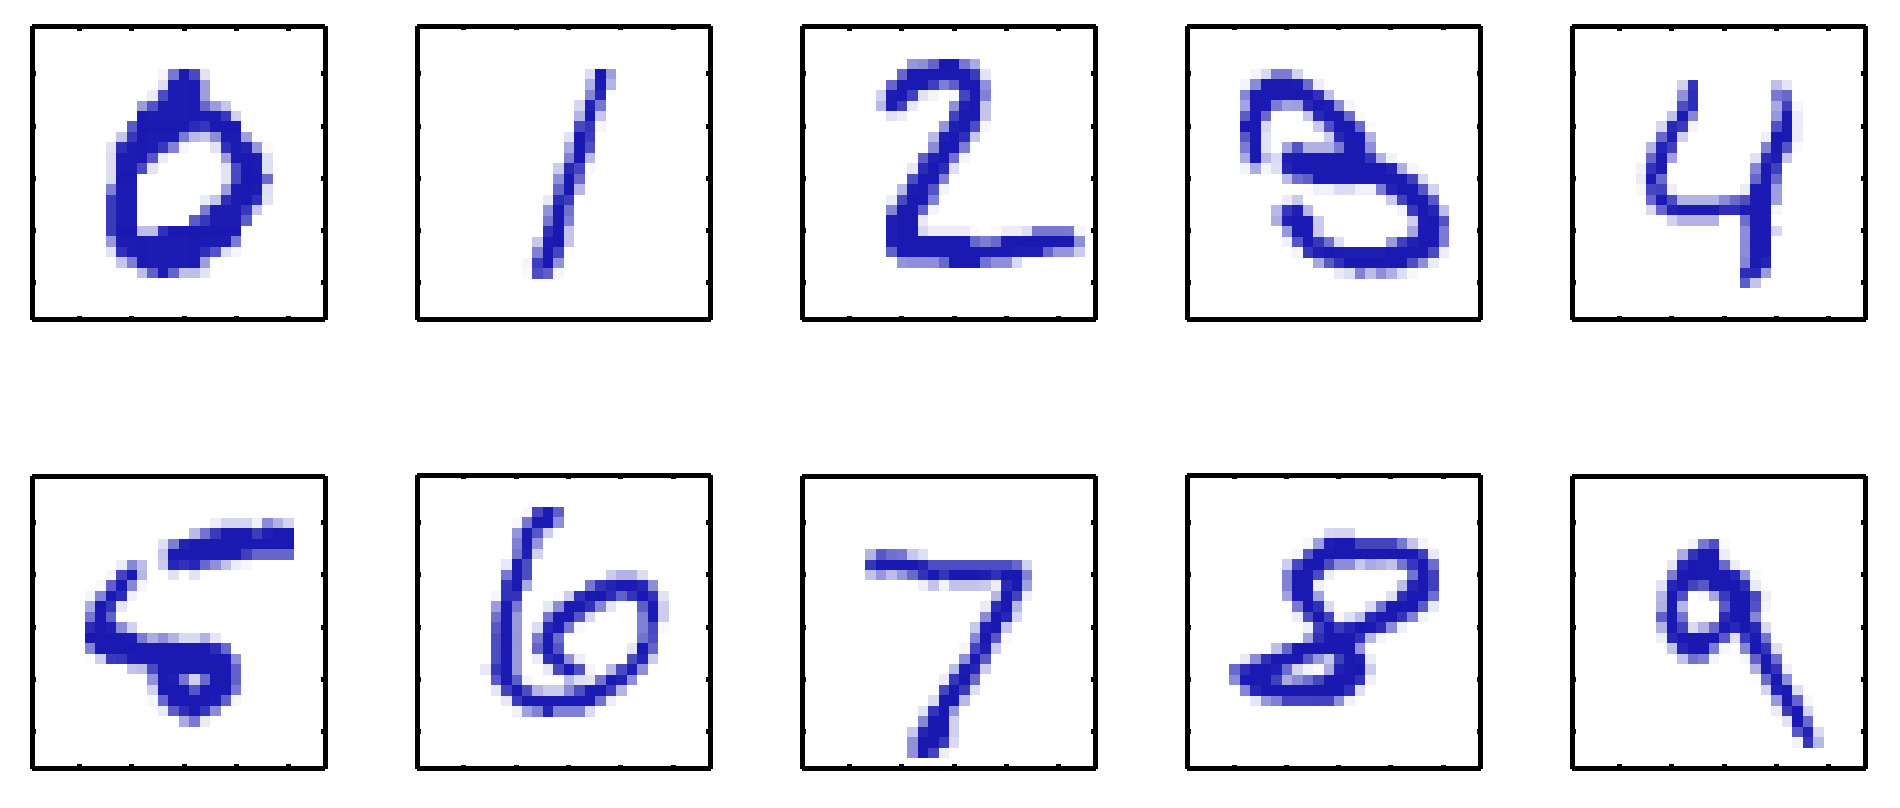
\includegraphics[scale=0.8]{Images/1-1.png}
		\captionsetup{font={small}}
		\caption{来自美国邮政编码的手写数字示例} 
		\label{fig:1-1}	
	\end{figure}
	\\
	\indent 通过机器学习,我们可以取得更好的结果。在机器学习方法中,我们会利用一个较大的训练集(training set)${\{ \textbf{x}_1,...,\textbf{x}_N\}}$来调节某个自适应模型的参数,训练集中包含有$N$个数字。训练集中的数字类别是已知的,一般要通过单独考察和手动标注。我们可以通过一个目标向量$\textbf{t}$来表示一个数字的类别,从而表征每个数字对应的特性。以向量形式表示类别的有效手段将在后文中进行论述。注意,对于每一个数字图像$\textbf{x}$,仅有一个这样的目标向量$\textbf{t}$。\\
	\indent 机器学习算法的运行结果可以表示为函数$\textbf{y}(\textbf{x})$,该函数将一个新的数字图像$\textbf{x}$作为输入并生成一个与目标向量形式相同的输出向量$\textbf{y}$。函数$\textbf{y}(\textbf{x})$的具体形式基于训练数据,确定于训练阶段,该阶段也被称为学习阶段。模型一旦完成训练,它就可以对测试集(test set)中新的数字图像进行分类。正确区分与训练实例不同的新实例的能力称为泛化(generalization)。在实际应用中,输入向量的多变性使得训练数据往往只能够覆盖到所有可能的输入变量中的一小部分,所以泛化是模式识别的核心目标之一。\\
	\indent 对于大部分的实际应用而言,初始的输入变量通常都是经过预处理的。我们将其变换到了新的向量空间,以期望在新的向量空间中,模式识别问题解决起来会变得容易一些。例如,在数字识别问题中,数字图像通常会经过变换和缩放,从而使每个数字都位于尺寸比较合适的方框中。这一做法大幅减少了每种数字的多变性,因为所有数字的位置和尺寸都变成相同的之后,随后的模式识别算法可以更加轻松地判断其类别。这种预处理步骤又会被称为特征提取(feature extraction)。注意,新的测试数据也必须经过和训练数据相同的预处理过程。\\
	\indent 为了提升计算的速度,也可能需要加入预处理的步骤。举例而言,如果我们的目标是在高分辨率的视频流中进行实时的人脸识别,计算机就必须在一秒钟内处理大量的像素,在复杂的模式识别算法中,用直接法表示像素,可能是算法根本无法计算的。所以,我们希望寻找出计算较快且具有较强区分度的特征,有效区分人脸与非人脸。这些特征就是接下来输入到模式识别算法的输入量。举例而言,我们可以评估矩形子区域上的图像灰度均值(Viola and Jones, 2004),这样的特征集合在快速人脸检测中非常有效。由于特征数量小于像素数量,所以这样的预处理是降维的一种形式。在预处理的过程中务必要小心,因为在此过程中通常会有信息被丢弃,而如果丢弃的信息对问题的解决具有重要的作用,那么整个系统的准确性都会大打折扣。\\
	\indent 如果训练数据中包含了输入向量及其对应的目标向量,那么这样的应用就称为监督学习(supervised learning)问题。类似于上文中数字识别案例的情况称为分类(classification)问题,分类问题的目标是对每个输入向量分配一个离散的类别,且类别的数量是有限的。如果希望得到的输出是由一个或多个连续变量组成的,那么就变成了一个回归(regression)问题。在化学生产过程中,以反应物浓度、温度和压力为输入,预测产量的问题就是回归问题的一个案例。\\
	\indent 除此之外还有一些其他形式的模式识别问题,这些问题中的训练数据仅仅是一个输入向量$\textbf{x}$的集合,没有任何对应的目标值。在这样的无监督学习(unsupervised learning)问题中,我们的目标可能是发现数据中相似实例的分组情况,这样的问题被称为聚类(clustering),或者是确定输入空间中数据的分布情况,这样的问题被称为密度估计(density estimation),亦或是将数据从高维空间投影到二维或三维中,进行数据的可视化(visualization)。\\
	\indent 最后,强化学习(reinforcement learning, Sutton and Barto, 1998)的目的是,在给定的情况下寻找到合适的行为,从而使获得的奖励达到最大。与监督学习相比,强化学习算法不会被告知哪些是最优的输出,而是必须在不断的实验试错中将最优输出分析出来。通常而言,在学习算法与环境的不断交互下,会产生一个状态和行为的序列。在多数情况下,当前的行为不仅仅会影响当前的奖励,还有可能在后续的任何时间节点对获得的奖励造成影响。举例而言,通过使用适当的强化学习技术,一个神经网络可以通过学习,使自己玩十五子棋游戏的能力达到很高的水平(Tesauro, 1994)。在这个问题中,神经网络将棋盘的当前情况和骰子投掷的结果一同作为输入,以具有威力的移动作为网络的输出。这是通过让神经网络与自己的复制品进行游戏来完成的,可能需要经历一百万次的游戏。一个主要的挑战是,十五子棋游戏可能包含很多的步骤,但只有在游戏结束时,才能以胜利或失败的形式收获奖励。所以,即使是好棋和坏棋并存的情况,奖励也必须归功于所有指向最终结果的步骤。这是信用分配问题的案例之一。强化学习的一般特征之一,是进行探索(exploration)和开发(exploitation)之间的制衡。在探索中,系统要尝试新的行为并验证其有效性;在开发中,系统要利用已知的行为,来获得更高的奖励。过多地关注探索或开发都会导致不良的结果。强化学习仍然是机器学习研究中的一个活跃领域,但本书中不包含对于强化学习的详细讨论。\\
	\indent 尽管每一个问题都需要各自的工具和技术,但对于所有的问题,解决它们的许多关键思想是相同的。本章的主要目标之一,就是以相对不太正式的方式,介绍一些很重要的概念,并利用一些简单的例子来解释它们。在这本书的后续内容中我们将看到,在现实世界中的模式识别应用里,相同的思想会再次出现在更加复杂的模型中。本章还提供了本书中即将使用的三个重要工具的介绍,即概率论、决策论和信息论。尽管听起来可能很吓人,但实际上它们很直观,而且如果希望使用机器学习技术在实际应用中得到最佳的效果,那么对它们有一个清晰的理解是不可或缺的。}

	\section{实例:多项式曲线拟合}
	\noindent{\color{red} \rule[10pt]{\textwidth}{0.1em}}
	\textnormal{
	\indent 我们从一个简单的回归问题开始,而且我们将在本章节中一直以这个问题为案例,介绍一系列关键的概念。假设我们对实值输入变量$x$进行观测,并希望利用观测结果来预测实值目标变量$t$。对于这样的目的,一个比较好的方法是研究一个基于人为生成数据的人造案例,因为这样我们可以完全获悉数据的详细生成过程,就可以与任何学习模型进行比较了。该案例中的数据是基于函数$\sin (2\pi x)$生成的,数据中的目标变量带有随机噪声,相关的内容可详见于附录A。\\
	\indent 假设我们现在有一个给定的训练集,其中包含有$N$个对$x$的观测,记作$\boldsymbol{\mathsf{x}} \equiv (x_1,...,x_N)^\mathrm{T}$, 同时有与之对应的目标变量$t$,记作$\boldsymbol{\mathsf{t}} \equiv (t_1,...,t_N)^\mathrm{T}$。图1.2展示了一个包含有$N=10$个数据点的训练集。图1.2中的输入数据集合$\boldsymbol{\mathsf{x}}$通过在[0,1]之间随机等可能地选取$x_n$来生成,其中$n=1,...,N$;而对于目标数据集合$\boldsymbol{\mathsf{t}}$,首先计算对应的函数值$\sin {(2 \pi x)}$,然后对每一个点加上一个较小且服从高斯分布的随机噪声,从而得到$x_n$对应的值$t_n$。高斯分布将在第1.2.4节中进行详细的介绍。通过这样的方式生成数据,可以获取很多真实数据集中的属性。换句话说,就是个别观测受到随机噪声干扰的数据中包含的潜在规律,而这些潜在规律就是我们希望学习的。随机噪声可能是由随机过程产生的,例如放射性衰变,但更多的情况下是由于存在缺乏观测的噪声源而形成的。
	\begin{figure}[ht]
		\centering
		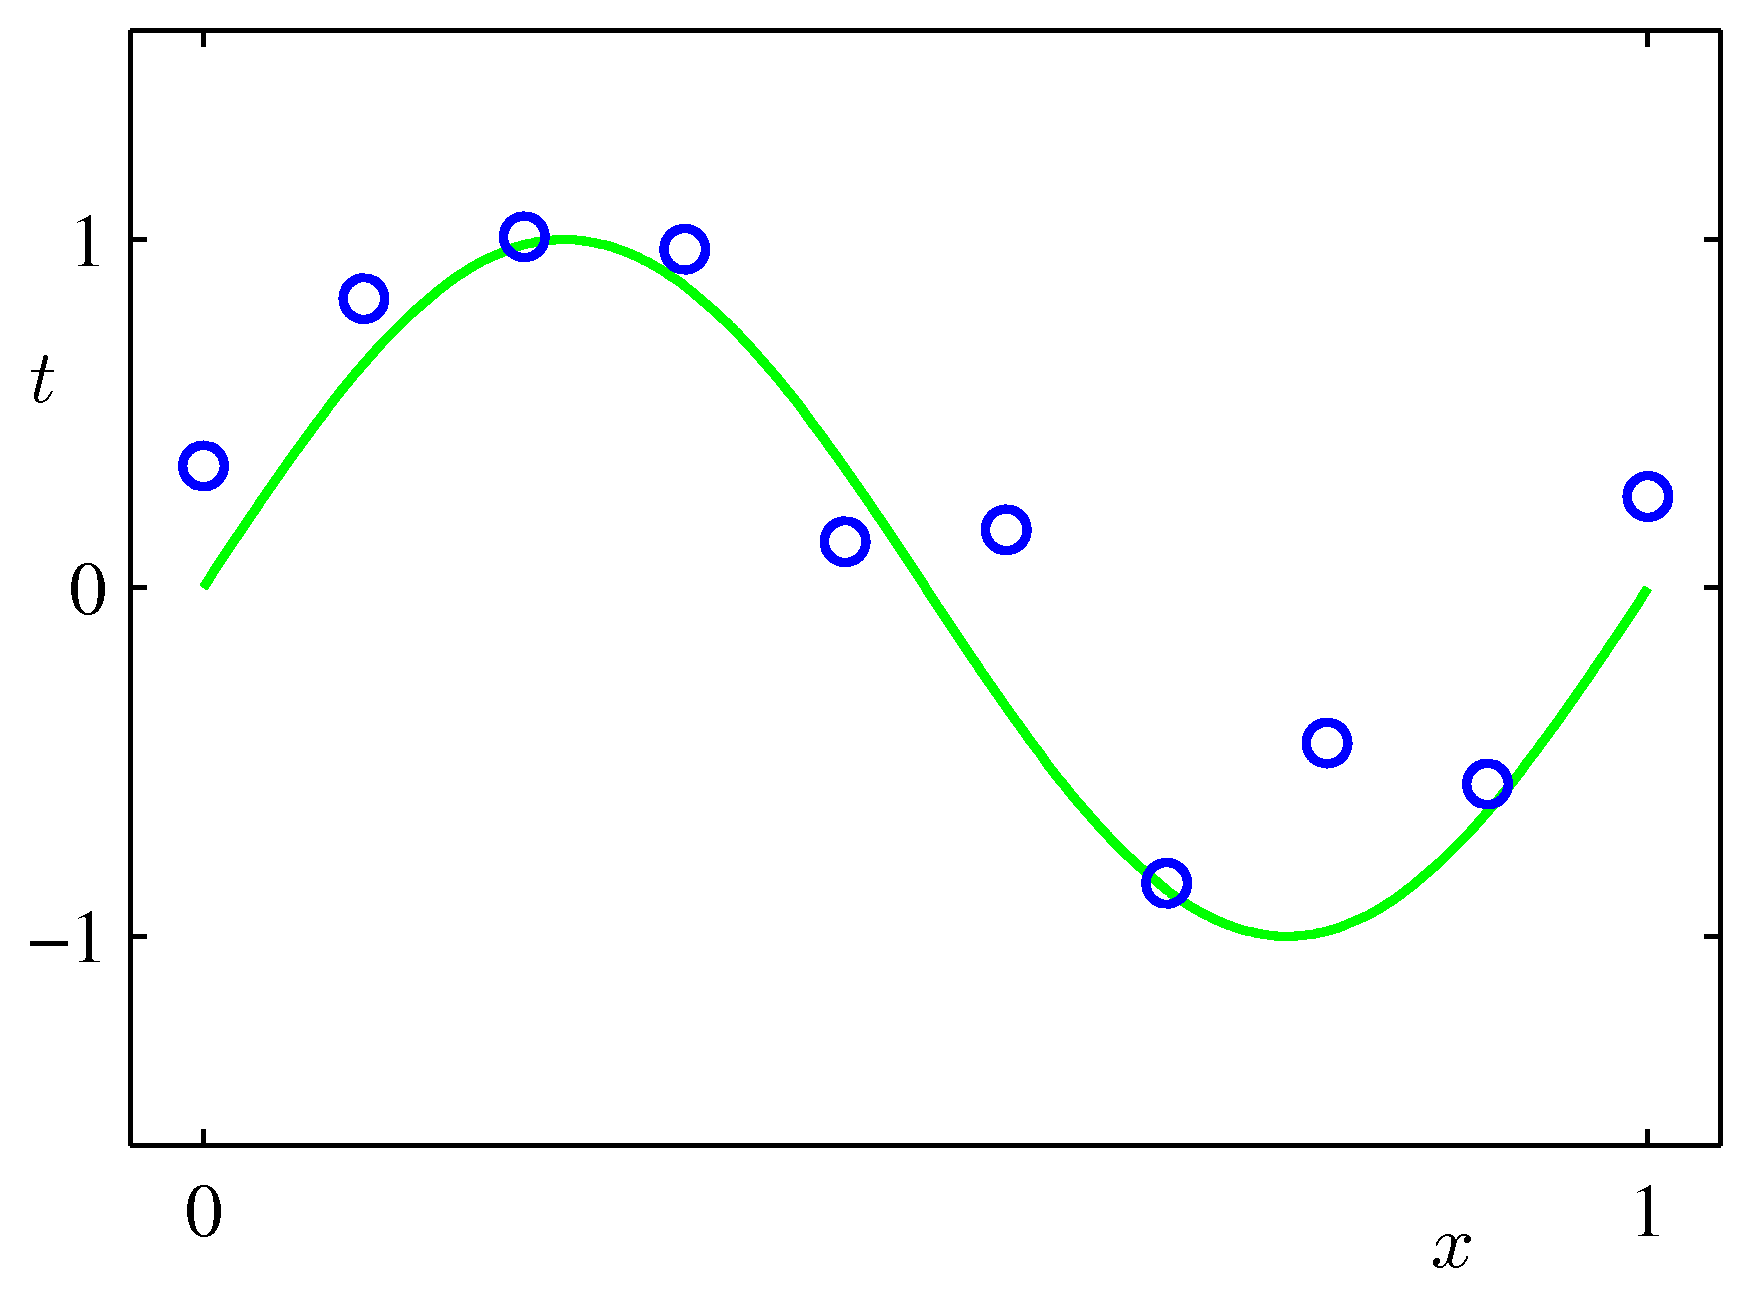
\includegraphics[scale=0.8]{Images/1-2.png}
		\captionsetup{font={small}}
		\caption{一个包含了$N=10$个点的训练集的图像,如图中蓝色圆圈所示,每个点都包括了输入变量$x$的观测值及其对应的目标变量值$t$。绿色的曲线表示用于生成数据的函数$\sin (2 \pi x)$。我们的目标是在绿色曲线未知的情况下,对于新的$x$值,预测其对应的$t$值。} 
		\label{fig:1-2}	
	\end{figure}
	\\
	\indent 我们的目标是对训练集加以利用,从而对新的输入变量$\hat{x}$进行其对应目标变量$\hat{t}$的预测。正如我们接下来将看到的一样,这个过程隐式地包含了发现数据中隐含的函数$\sin (2 \pi x)$。这似乎是一个困难的事情,因为我们需要利用一个有限的数据集将这个隐含的函数归纳出来。而且,我们得到的观测数据是受到噪声干扰的,于是对于给定的$\hat x$,估计出来的$\hat t$是具有不确定性的。为了研究这种不确定性,第1.2节中的概率论提供了一个可以精确、定量表示不确定性的框架;同时,第1.5节中的决策论使得我们可以利用不确定性的概率表示进行适当标准下的最优预测。\\
	\indent 不过现在我们也将不太正式地继续分析下去,研究一个基于曲线拟合的简单方法。特别地,我们将使用如下形式的多项式函数进行数据拟合:
	\begin{equation}
		y(x,\mathbf{w})= w_0 + w_1 x + w_2 x^2 + ... + w_M x^M = \sum_{j=0}^M w_j x^j
	\end{equation}
	其中$M$是多项式的阶(order),$x^j$表示变量$x$的$j$次方。多项式系数$w_0,...,w_m$可以集合在一起,用向量$\mathbf{w}$表示。需要注意的是,尽管多项式函数$y(x,\mathbf{w})$是一个关于$x$的非线性函数,但它也是一个关于系数$\mathbf{w}$的线性函数。关于未知参数的线性函数,比如这个多项式函数,被称为线性模型(linear models)。线性模型具有很多重要的性质,将在第3章和第4章中详细介绍。\\
	\indent 我们可以根据训练数据调整多项式函数,从而确定这些系数的值。这项任务可以通过误差函数(error function)的最小化来完成。误差函数衡量的是对于任意的$\mathbf{w}$,函数值$y(x,\mathbf{w})$与训练集数据点之间的差距。一种广泛应用而且比较简单的误差函数是求取每一个数据点$x_n$上的预测值$y(x_n,\mathbf{w})$与对应的目标变量$t_n$差值的平方和,于是我们需要将如下函数进行最小化:
	\begin{equation}
	E(\mathbf{w}) = \frac{1}{2} \sum_{n=1}^N \{y(x_n,\mathbf{w}) - t_n\}^2
	\end{equation}
	其中的系数$1/2$是为了接下来计算的方便添加的。选择这样的误差函数的理由也将在本章节稍后的内容中进行介绍。现在我们只需注意到它是一个非负函数,当且仅当所有训练数据点都在函数$y(x,\mathbf{w})$上时,误差函数的值为0。平方和误差函数的几何解释如图1.3所示。
	\begin{figure}[ht]
		\centering
		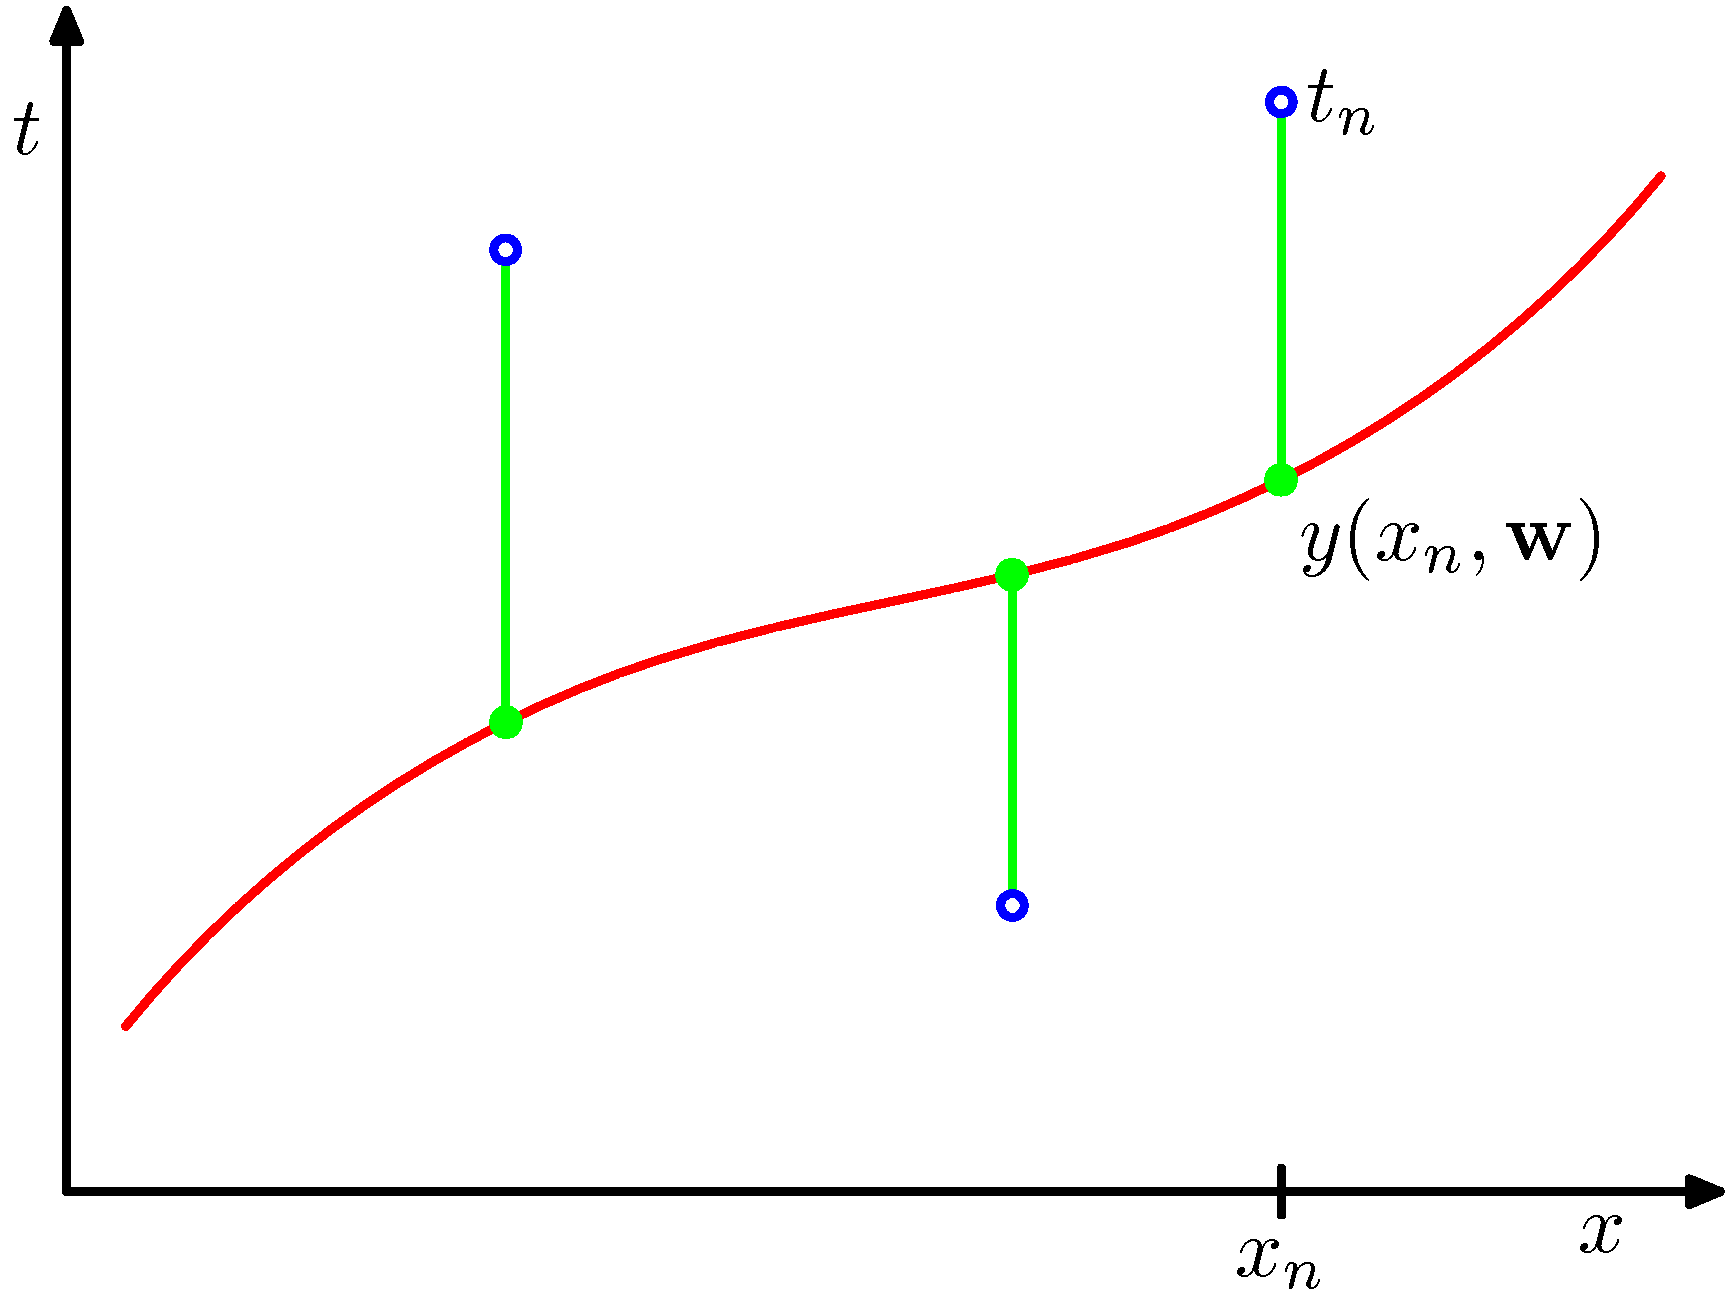
\includegraphics[scale=0.8]{Images/1-3.png}
		\captionsetup{font={small}}
		\caption{误差函数(1.2)对应每个数据点与函数$y(x, \mathbf{w})$之间相差距离(绿色垂直线)的平方和(的一半)。} 
		\label{fig:1-3}	
	\end{figure}
	\\
	\indent 我们可以通过选择使得$E(\mathbf{w})$尽可能小的$\mathbf{w}$来解决这个曲线拟合问题。由于误差函数对于系数$\mathbf{w}$是一个二次函数,所以误差函数的导数对于$\mathbf{w}$是线性的,所以误差函数最小化的结果是唯一的,可以求取其解析解$\mathbf{w^\star}$。最终得到的结果为多项式函数$y(x,\mathbf{w^\star})$。\color{red} \textbf{——习题 1.1}\\
	\color{black}
	\indent 还有一个问题是选择多项式的阶数$M$。它的背后是一个重要的问题——模型对比(model comparison,或称为模型选择,model selection)。在图1.4中,我们展示了在阶数$M=0,1,3$和$9$时,对于图1.2所示的数据集的拟合结果。
	\begin{figure}[ht]
		\begin{minipage}[t]{0.5\linewidth}
		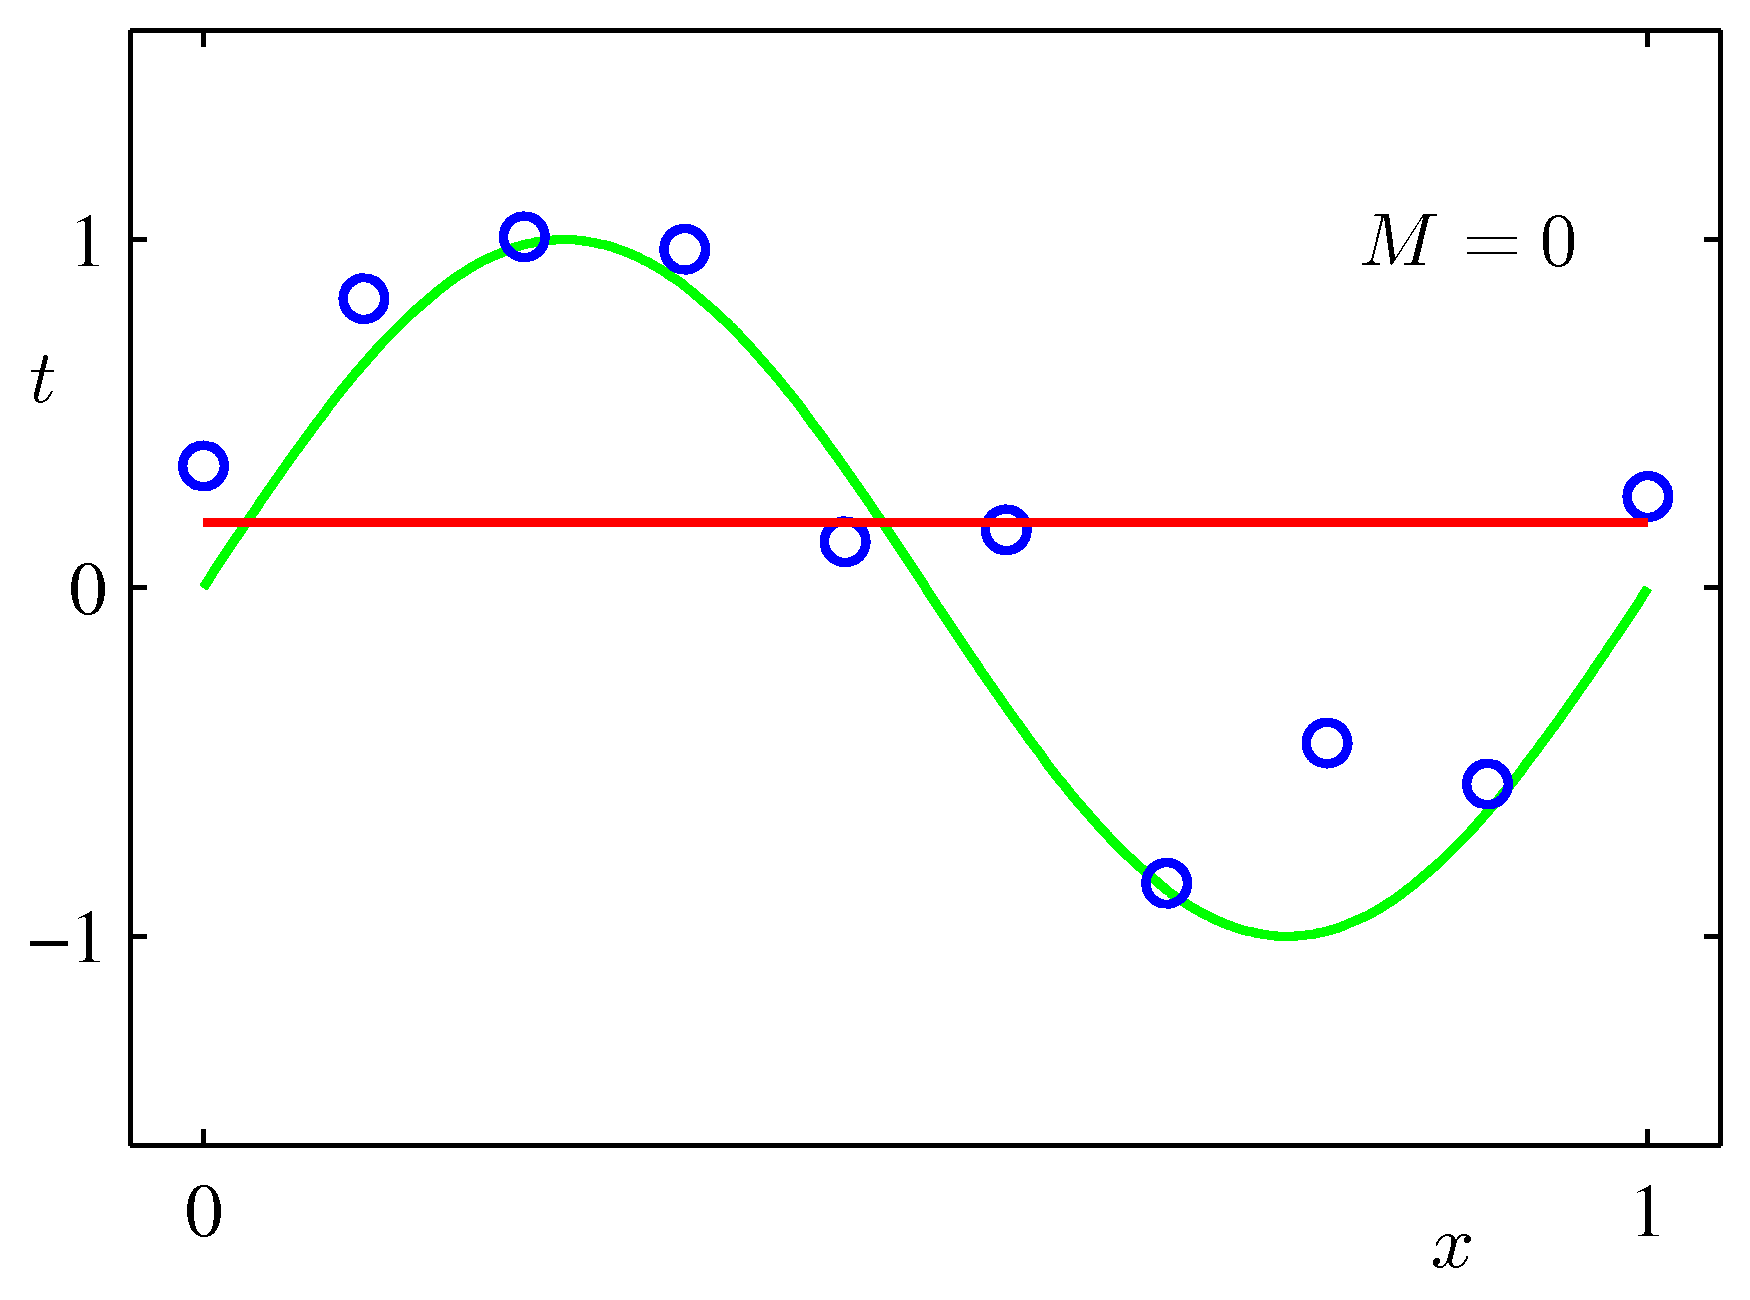
\includegraphics[scale=0.8]{Images/1-4a.png}
		\label{fig:1-4a}
		\end{minipage}
		\begin{minipage}[t]{0.5\linewidth}
		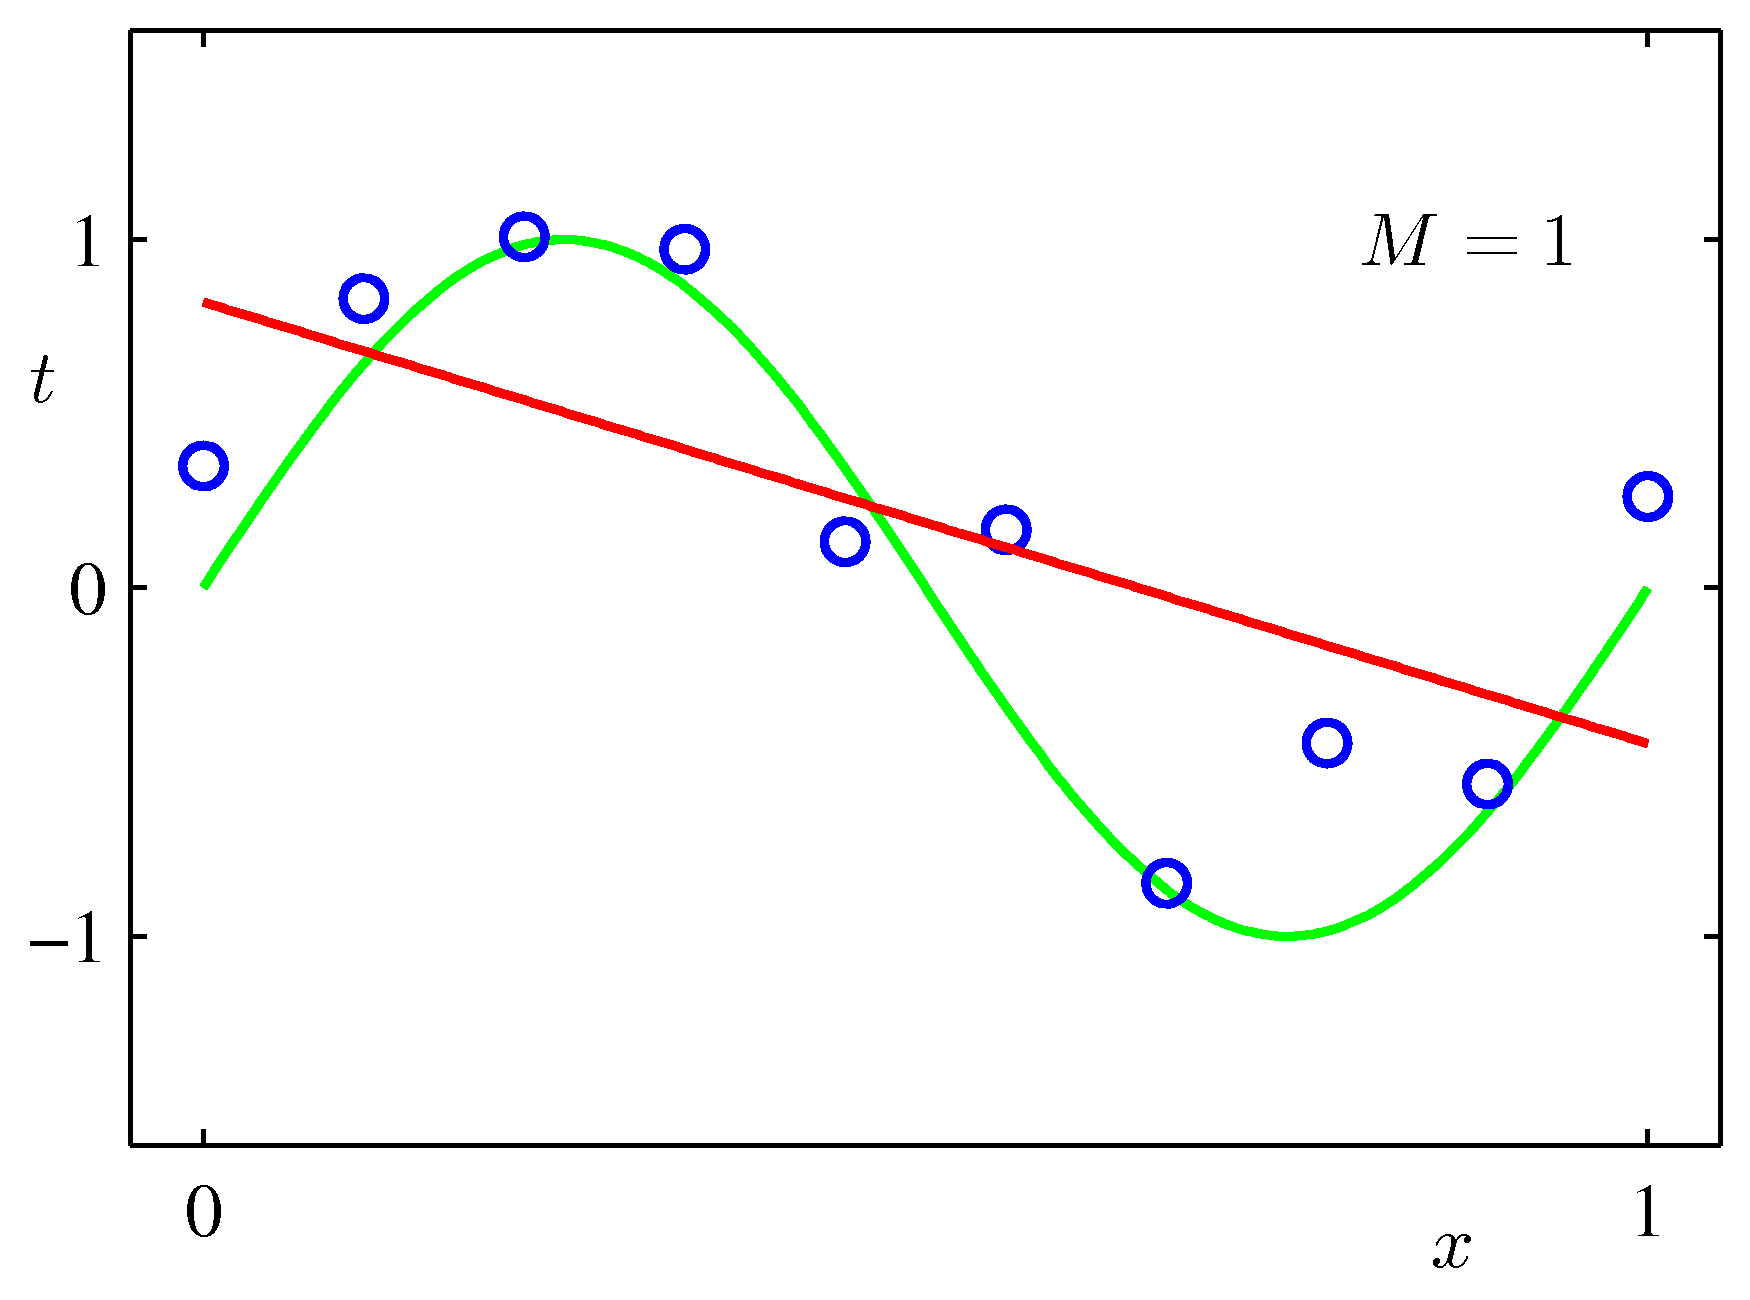
\includegraphics[scale=0.8]{Images/1-4b.png}
		\label{fig:1-4b}
		\end{minipage} \\
		\begin{minipage}[t]{0.5\linewidth}
		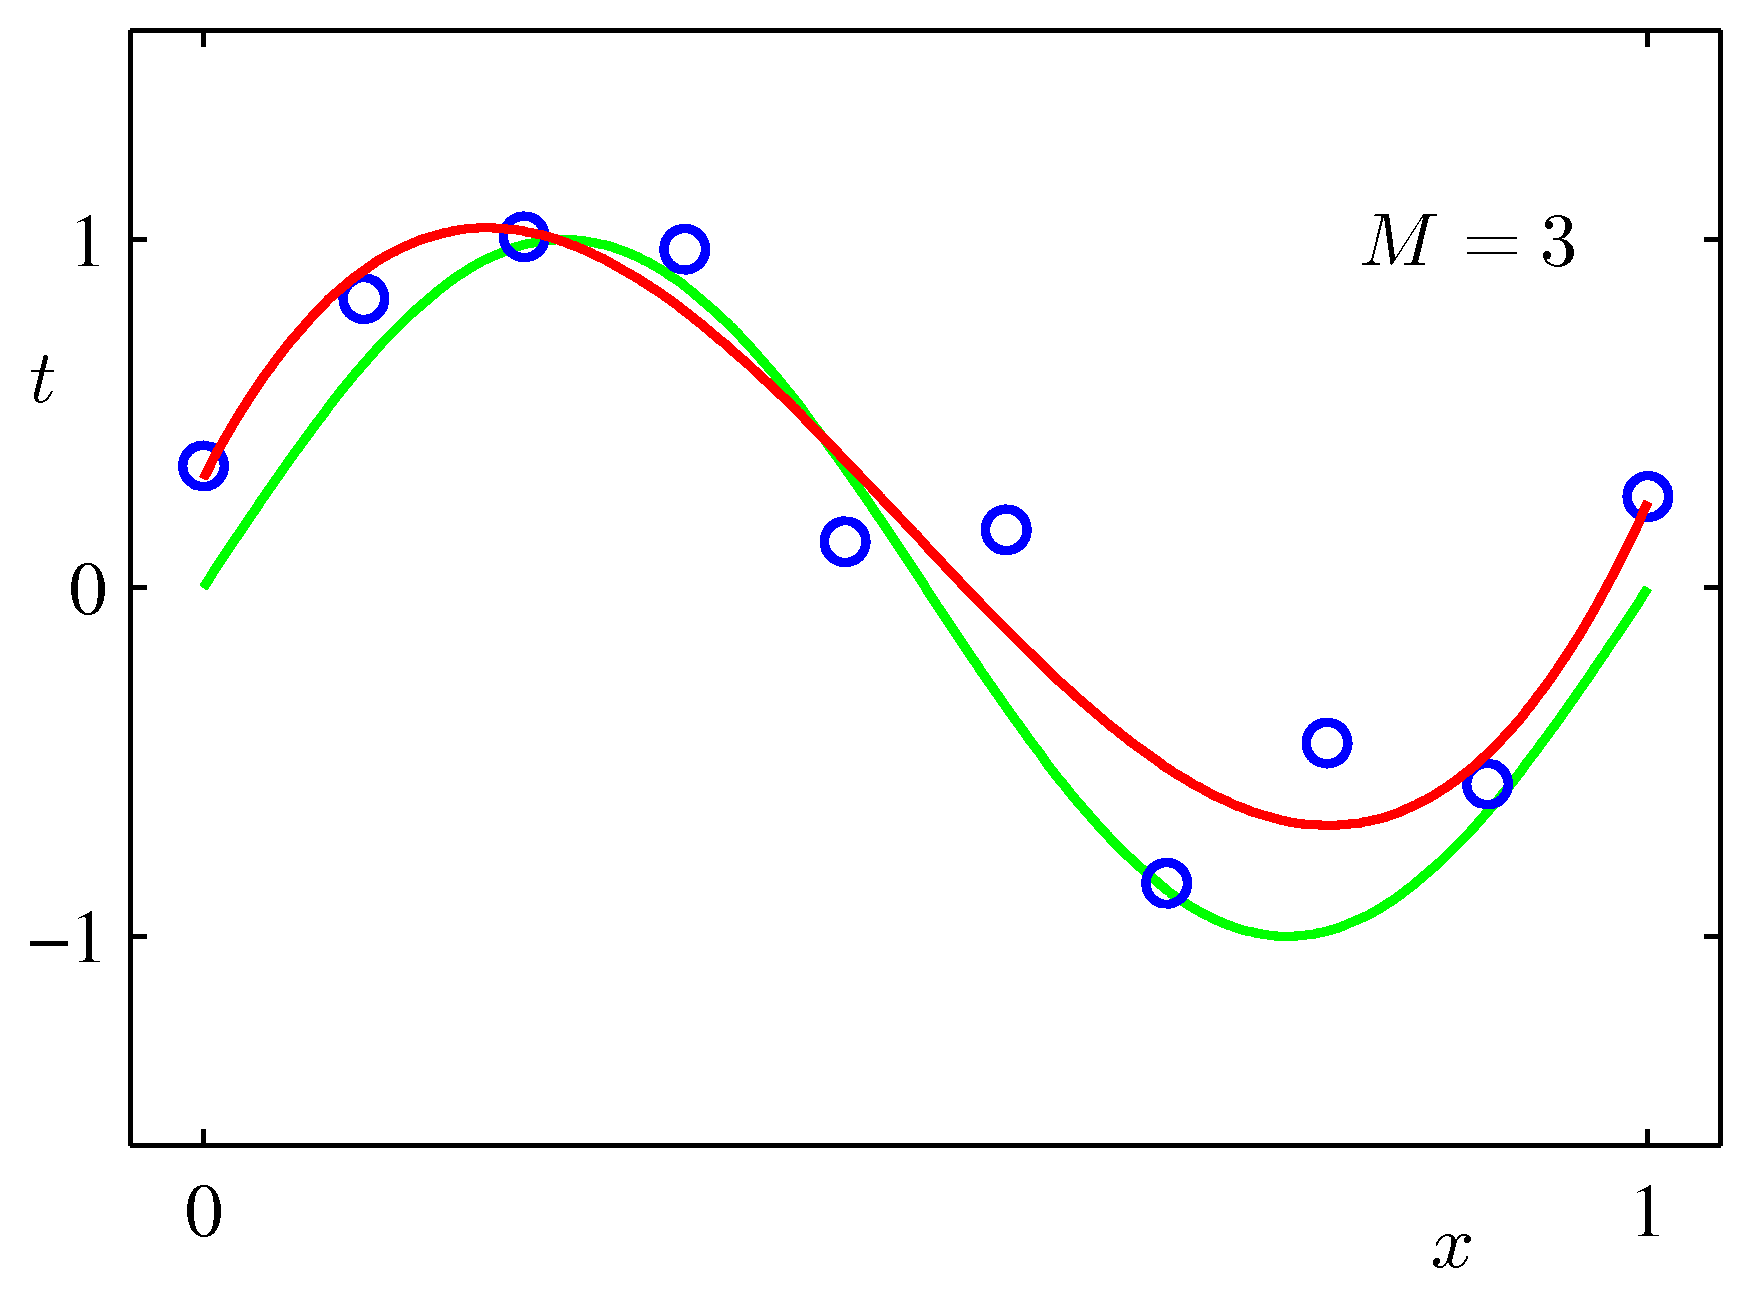
\includegraphics[scale=0.8]{Images/1-4c.png}
		\label{fig:1-4c}
		\end{minipage}
		\begin{minipage}[t]{0.5\linewidth}
		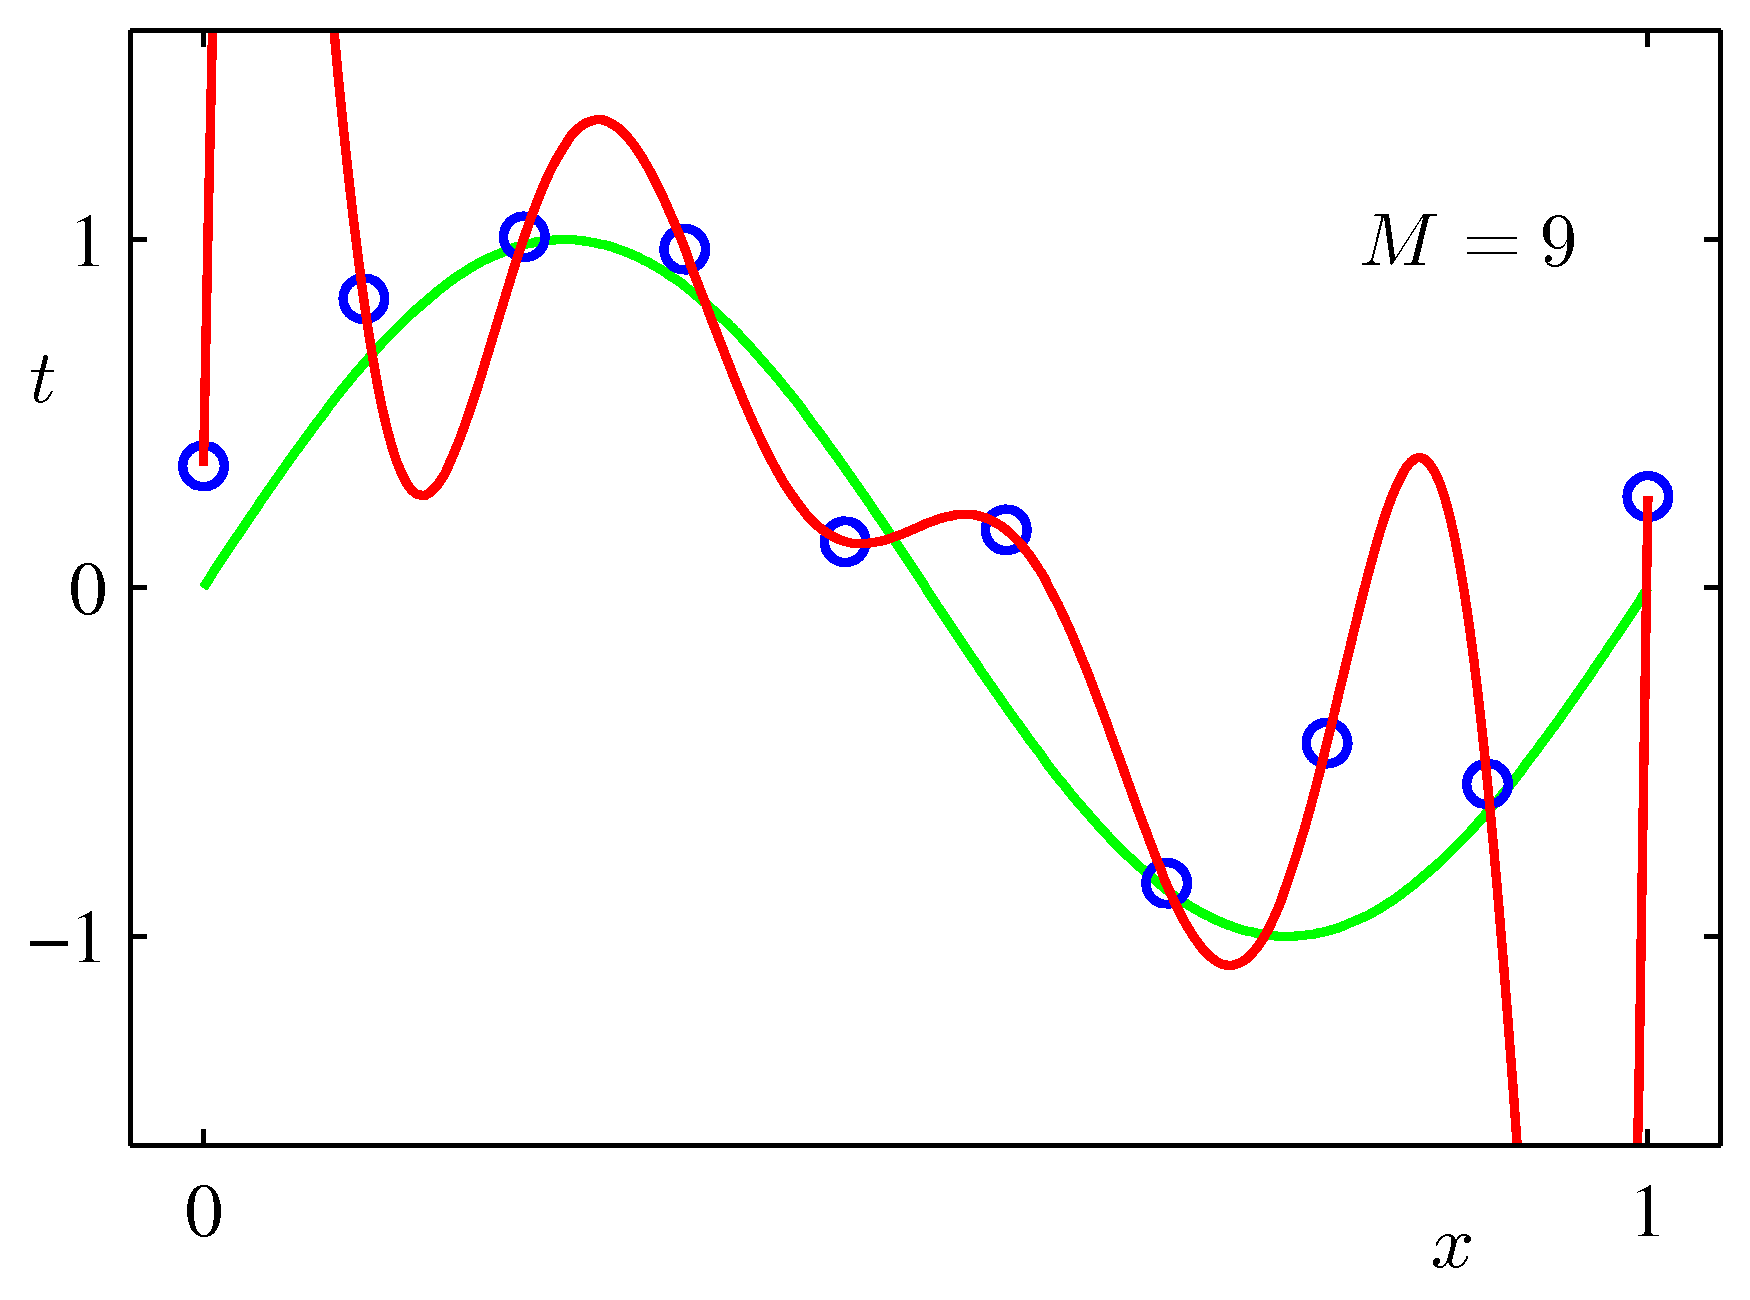
\includegraphics[scale=0.8]{Images/1-4d.png}
		\label{fig:1-4d}
		\end{minipage}
		\captionsetup{font={small}}
		\caption{在$M$变化时的拟合图1.2所示数据的多项式图像(红色曲线)。}
	\end{figure}
	\\
	\indent 我们注意到,在函数为常数($M=0$)和一阶函数($M=1$)时,对于数据的拟合效果相当差,几乎没法表达函数$\sin (2 \pi x)$。三阶函数($M=3$)看起来是本例中对函数$\sin (2 \pi x)$最佳的拟合。当我们再提高多项式的阶数,到了很高的阶数($M=9$)时,我们得到了一个特别好的拟合结果。其实在这种情况下,所有数据点都在多项式函数上,所以$E(\mathbf{w^\star})=0$。然而,这样的拟合结果振荡得很厉害,而且对函数$\sin (2 \pi x)$的表达同样很差。这样的情况我们称之为过拟合(over-fitting)。\\
	\indent 前面我们已经提到了,我们的目标是让模型具有较好的泛化能力,从而对新数据也有准确的预测能力。我们可以利用一个独立的测试集来获得$M$对泛化性能影响程度的定量分析。该测试集中有100个数据点,这些数据点的生成方式与训练集完全相同,但目标值中包含的随机噪声有所不同。对任意的$M$,我们可以根据(1.2)估计$E(\mathbf{w^\star})$关于训练数据的残差值,同样地我们也可以估计$E(\mathbf{w^\star})$关于测试数据的残差。有时使用均方根误差(RMS error,root-mean-square error)更加方便,由以下公式定义:
	\begin{equation}
	E_{\textnormal{RMS}}=\sqrt{2E(\mathbf{w^\star})/N}
	\end{equation}
	其中除以$N$的做法是为了对于不同大小的数据集进行公平的分析,而平方根可以保证$E_{\textnormal{RMS}}$使用与目标变量$t$相同的比例(和单位)进行误差的衡量。在$M$取不同的值时,训练集和测试集的RMS误差图如图1.5所示。测试集的误差刻画了对于新的数据$x$产生的预测值$t$的准确程度。从图1.5可知,较小的$M$值会导致较大的测试集误差,这可以归因于这时的多项式不够灵活,以致于难以准确刻画函数$\sin (2 \pi x)$的振荡情况。在$3 \leqslant M \leqslant 8$范围内的$M$值可以使测试集误差变得很小,它们对函数$\sin (2 \pi x)$也形成了比较合理的近似表达,比如如图1.4所示的$M=3$的情况。\\
	\indent 当$M=9$时,似乎是达到了我们最期望的情况,训练集误差变成了$0$,因为此时的多项式包含了10个自由度,对应于10个系数:$w_0,...,w_9$,所以可以针对训练集中的10个数据点进行精确的调整。然而,测试集的误差却变得特别大,正如图1.4中所示的那样,对应的函数$y(x,\mathbf{w^\star})$表现出了强烈的振荡。
	\begin{figure}[H]
		\centering
		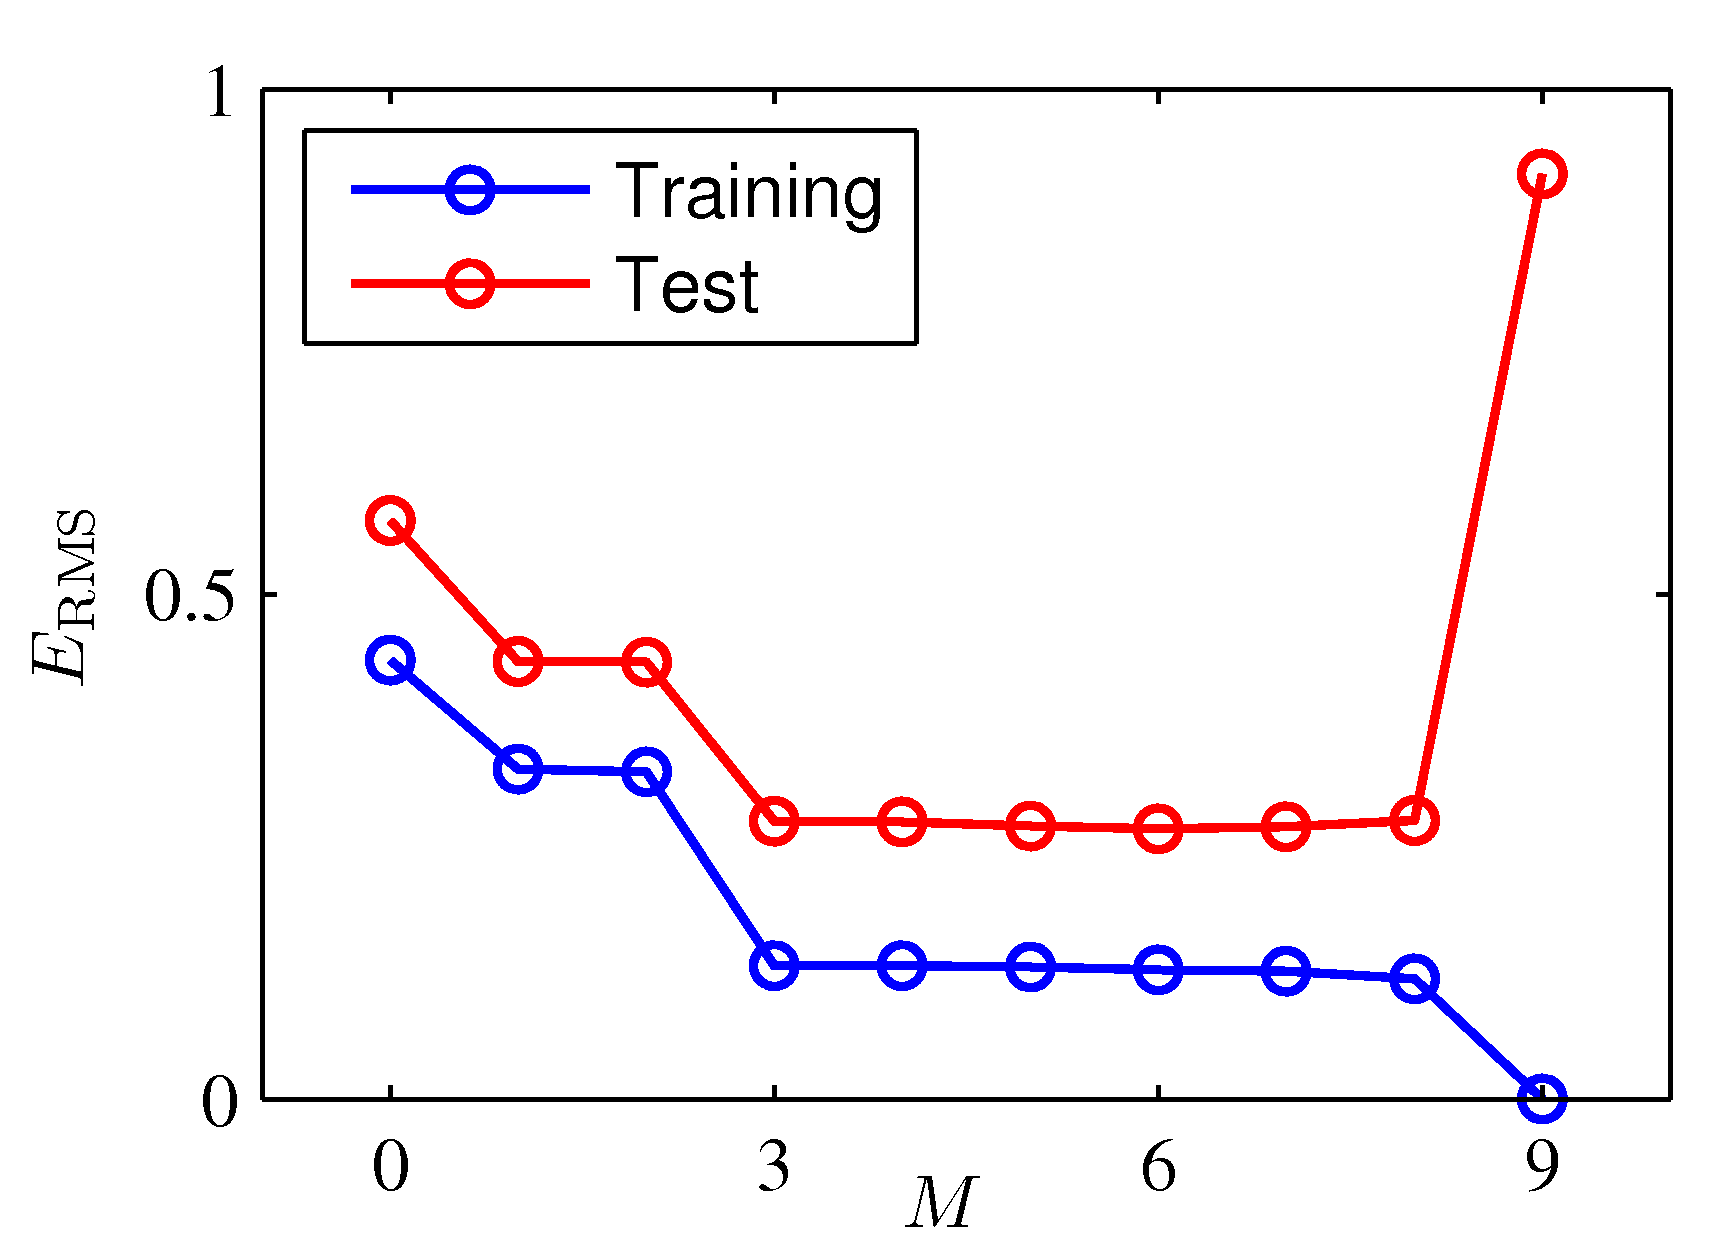
\includegraphics[scale=0.8]{Images/1-5.png}
		\captionsetup{font={small}}
		\caption{在不同的$M$值下,在训练集和独立测试集上根据(1.3)计算的均方根误差图像。} 
		\label{fig:1-5}	
	\end{figure}
	\indent 这看起来似乎有点自相矛盾,因为某个阶数一定的多项式应该包含了比它低阶的多项式,因为低阶多项式是高阶多项式的一种特殊情况。$M=9$的多项式至少应该取得与$M=3$的情况比较相似的结果。而且我们可以假设,对于新数据最优的预测函数为$\sin (2 \pi x)$(稍后我们会看到确实是这样的),因为数据就是从这个函数生成的。我们知道函数$\sin (2 \pi x)$的幂级数展开包含了任意阶数的项,随着$M$的增长,我们应该得到更好的近似结果。\\
	\indent 我们可以通过研究不同阶数的多项式中系数$\mathbf{w^\star}$的值来得到更加深刻的分析,如表1.1所示。可以发现,随着$M$的增大,系数通常也会随之变大。特别地,在$M=9$时,系数需要取到相当大才能对数据形成精确的拟合,而且还是正值和负值都有。于是在每个数据点之间,尤其是接近整个训练集数据范围边缘的地方,函数发生了剧烈的振荡,如图1.4所示。直观而言,这种情况的出现是因为在$M$较大的时候多项式实在太过灵活,以至于在拟合的过程中把目标值中包含的随机噪声也考虑了进去。	\\
	\indent 另外还有一个比较有意思的事情,在数据集规模发生变化时,模型的性能也会随之变化,如图1.6所示。我们可以看到,对于给定的模型复杂度,随着数据集规模的增大,过拟合问题变得越来越不严重。换句话说,数据集越大,就可以用越复杂的(也就是越灵活的)模型来进行数据拟合。一个比较粗略的启发是,数据集中数据点的数量应不小于模型中可调节参数数量的若干倍(比如5倍、10倍)。然而,我们即将在第3章中看到,参数的数量并不一定是模型复杂度最合适的度量。\\
	\indent 不过另外有件事让人相当不爽,那就是必须根据训练集的规模来限制模型中参数的数量。明明应该根据问题的复杂程度来确定模型的复杂度,这样才更加合理。我们将看到,使用最小二乘法寻找模型参数是最大似然(maximum likelihood,将在第1.2.5节中进行讨论)的一种特殊情形,而过拟合问题可以被理解成最大似然的一般
	\begin{table}
		\centering
		\begin{tabular}{c|rrrr}
			\ & $M=0$ & $M=1$ & $M=3$ & $M=9$ \\
			\hline
			$w_0^\star$ & 0.19 & 0.82 & 0.31 & 0.35\\
			$w_1^\star$ & \  & -1.27 & 7.99 & 232.37\\
			$w_2^\star$ & \  & \  & -25.43 & -5321.83\\
			$w_3^\star$ & \  & \  & 17.37 & 48568.31\\
			$w_4^\star$ & \  & \  & \  & -231639.30\\
			$w_5^\star$ & \  & \  & \  & 640042.26\\
			$w_6^\star$ & \  & \  & \  & -1061800.52\\
			$w_7^\star$ & \  & \  & \  & 1042400.18\\
			$w_8^\star$ & \  & \  & \  & -557682.99\\
			$w_9^\star$ & \  & \  & \  & 125201.43\\
		\end{tabular}
		\captionsetup{font={small}}
		\caption{不同阶数的多项式中的系数$\mathbf{w^\star}$。显而易见,随着阶数的增长,系数的绝对值也在飞速增长。}
	\end{table}
	\begin{figure}[ht]
		\begin{minipage}[t]{0.5\linewidth}
		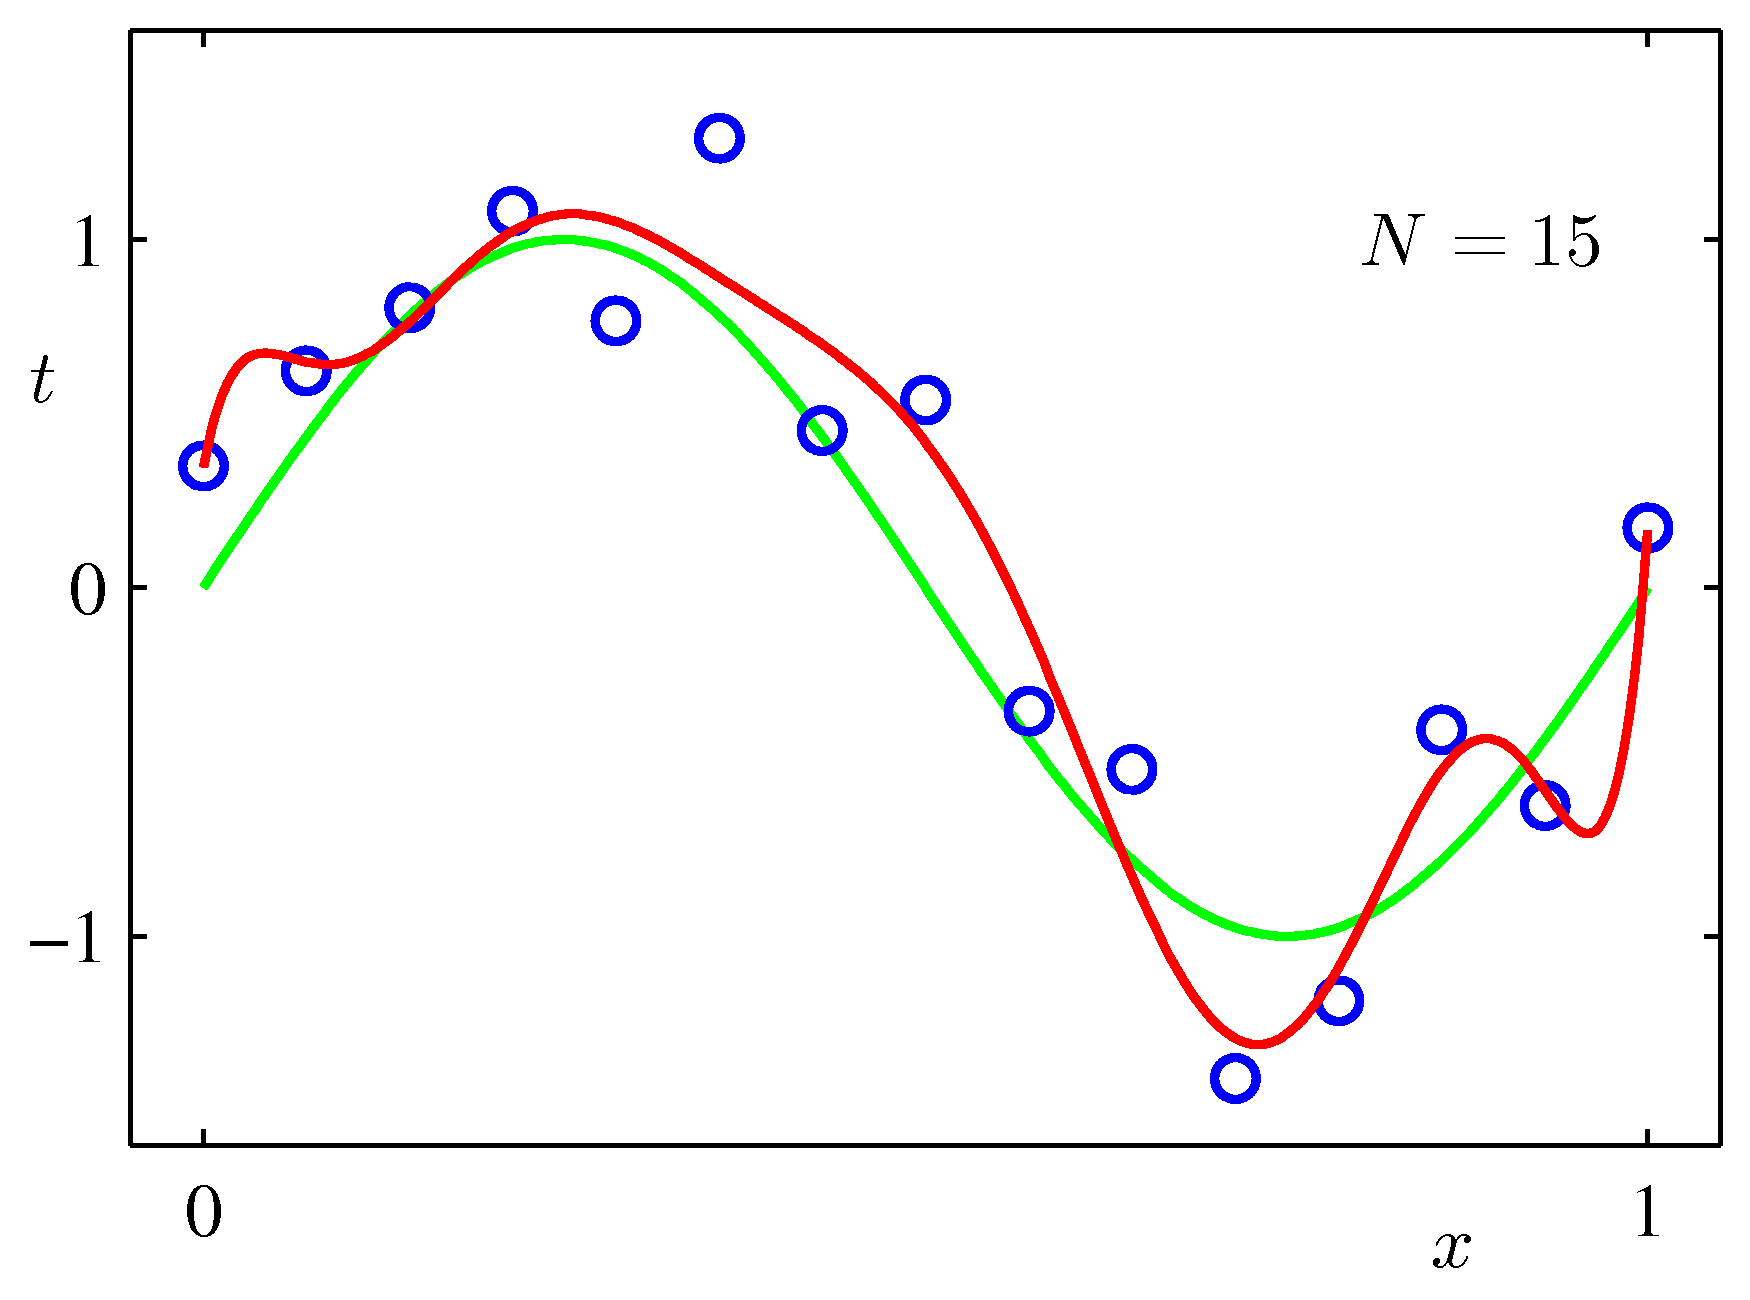
\includegraphics[scale=0.8]{Images/1-6a.png}
		\label{fig:1-6a}
		\end{minipage}
		\begin{minipage}[t]{0.5\linewidth}
		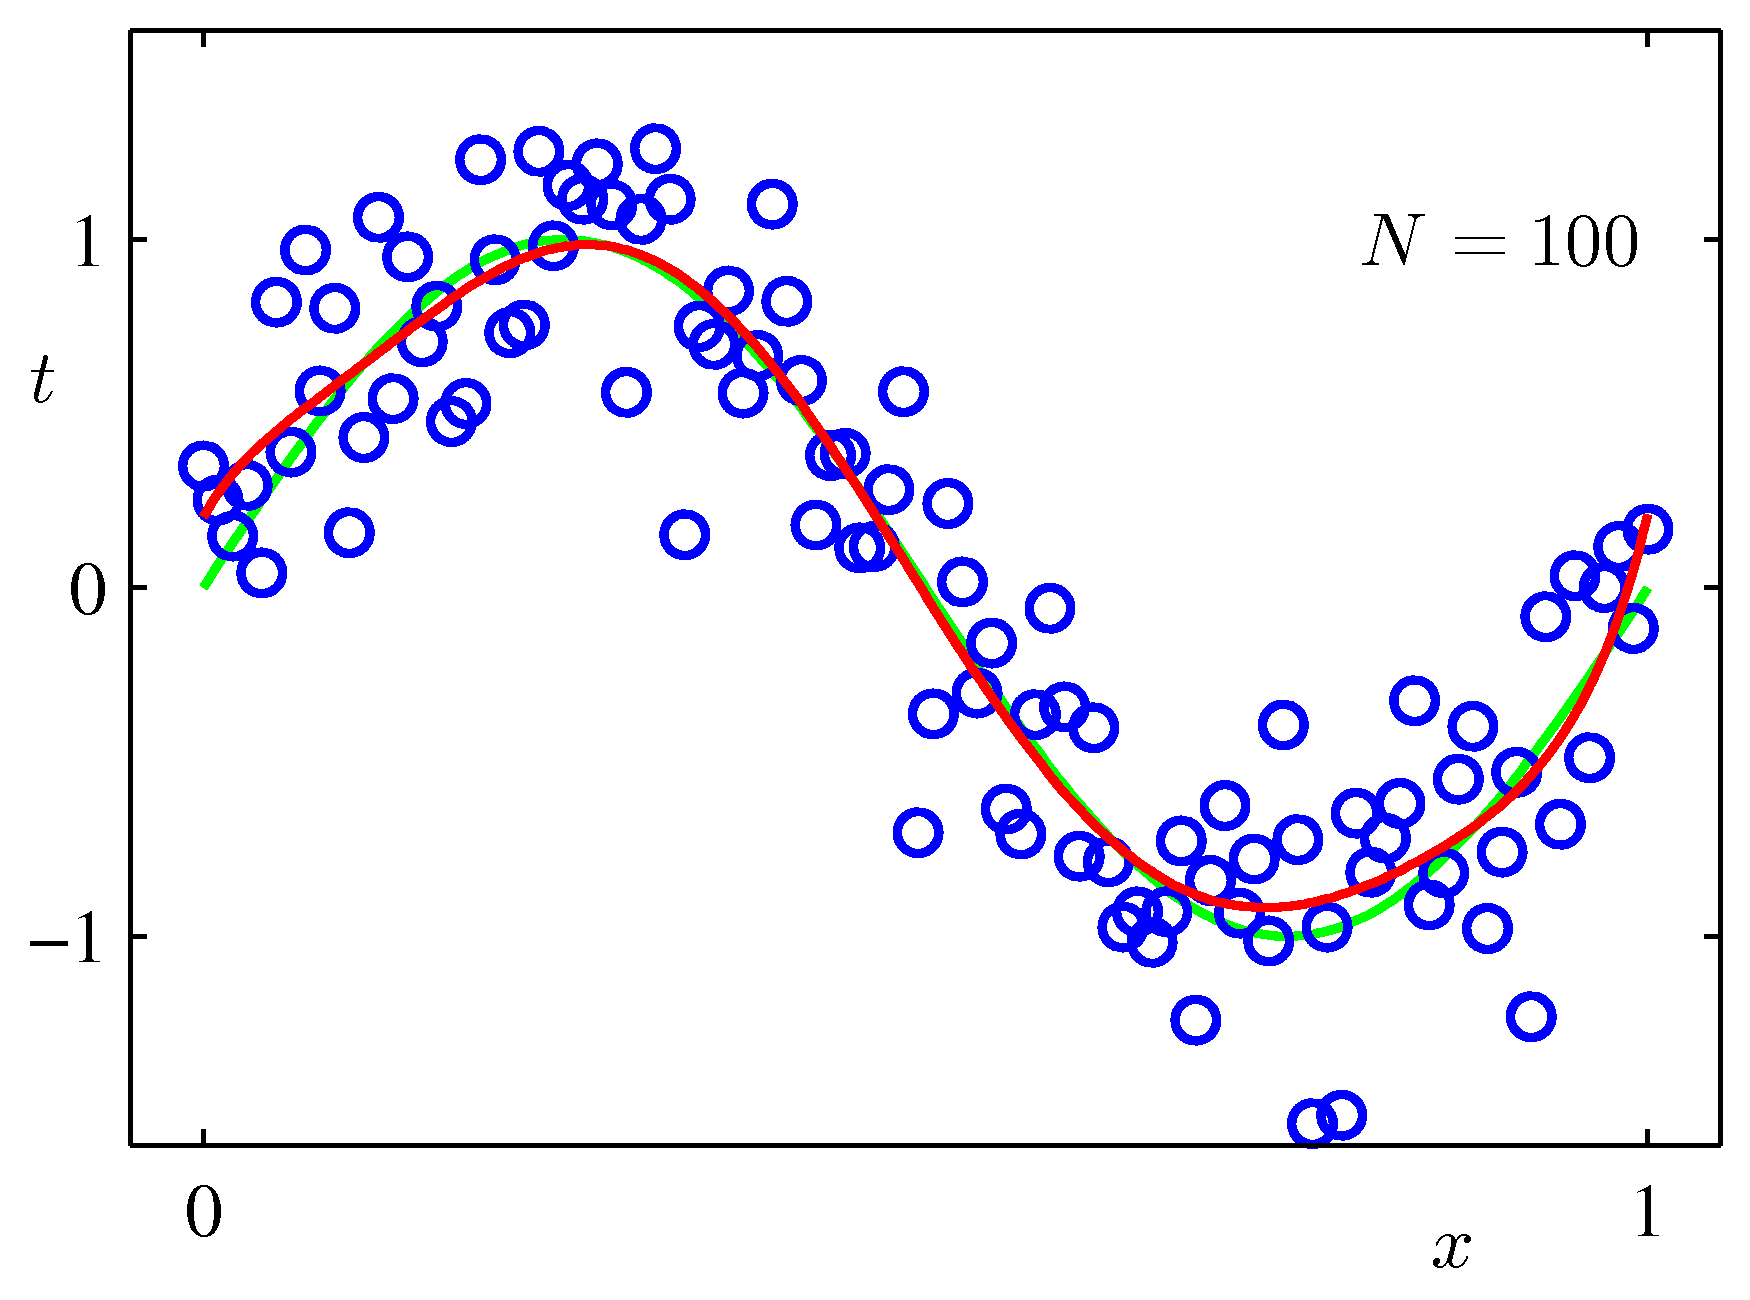
\includegraphics[scale=0.8]{Images/1-6b.png}
		\label{fig:1-6b}
		\end{minipage}
		\captionsetup{font={small}}
		\caption{在$M=9$的情况下,基于$N=15$(左)和$N=100$(右)个数据点进行平方和误差函数最小化得到的结果图像。我们可以看到,数据集规模的增加削弱了过拟合的问题。}
	\end{figure}
	\begin{figure}[H]
		\begin{minipage}[t]{0.5\linewidth}
		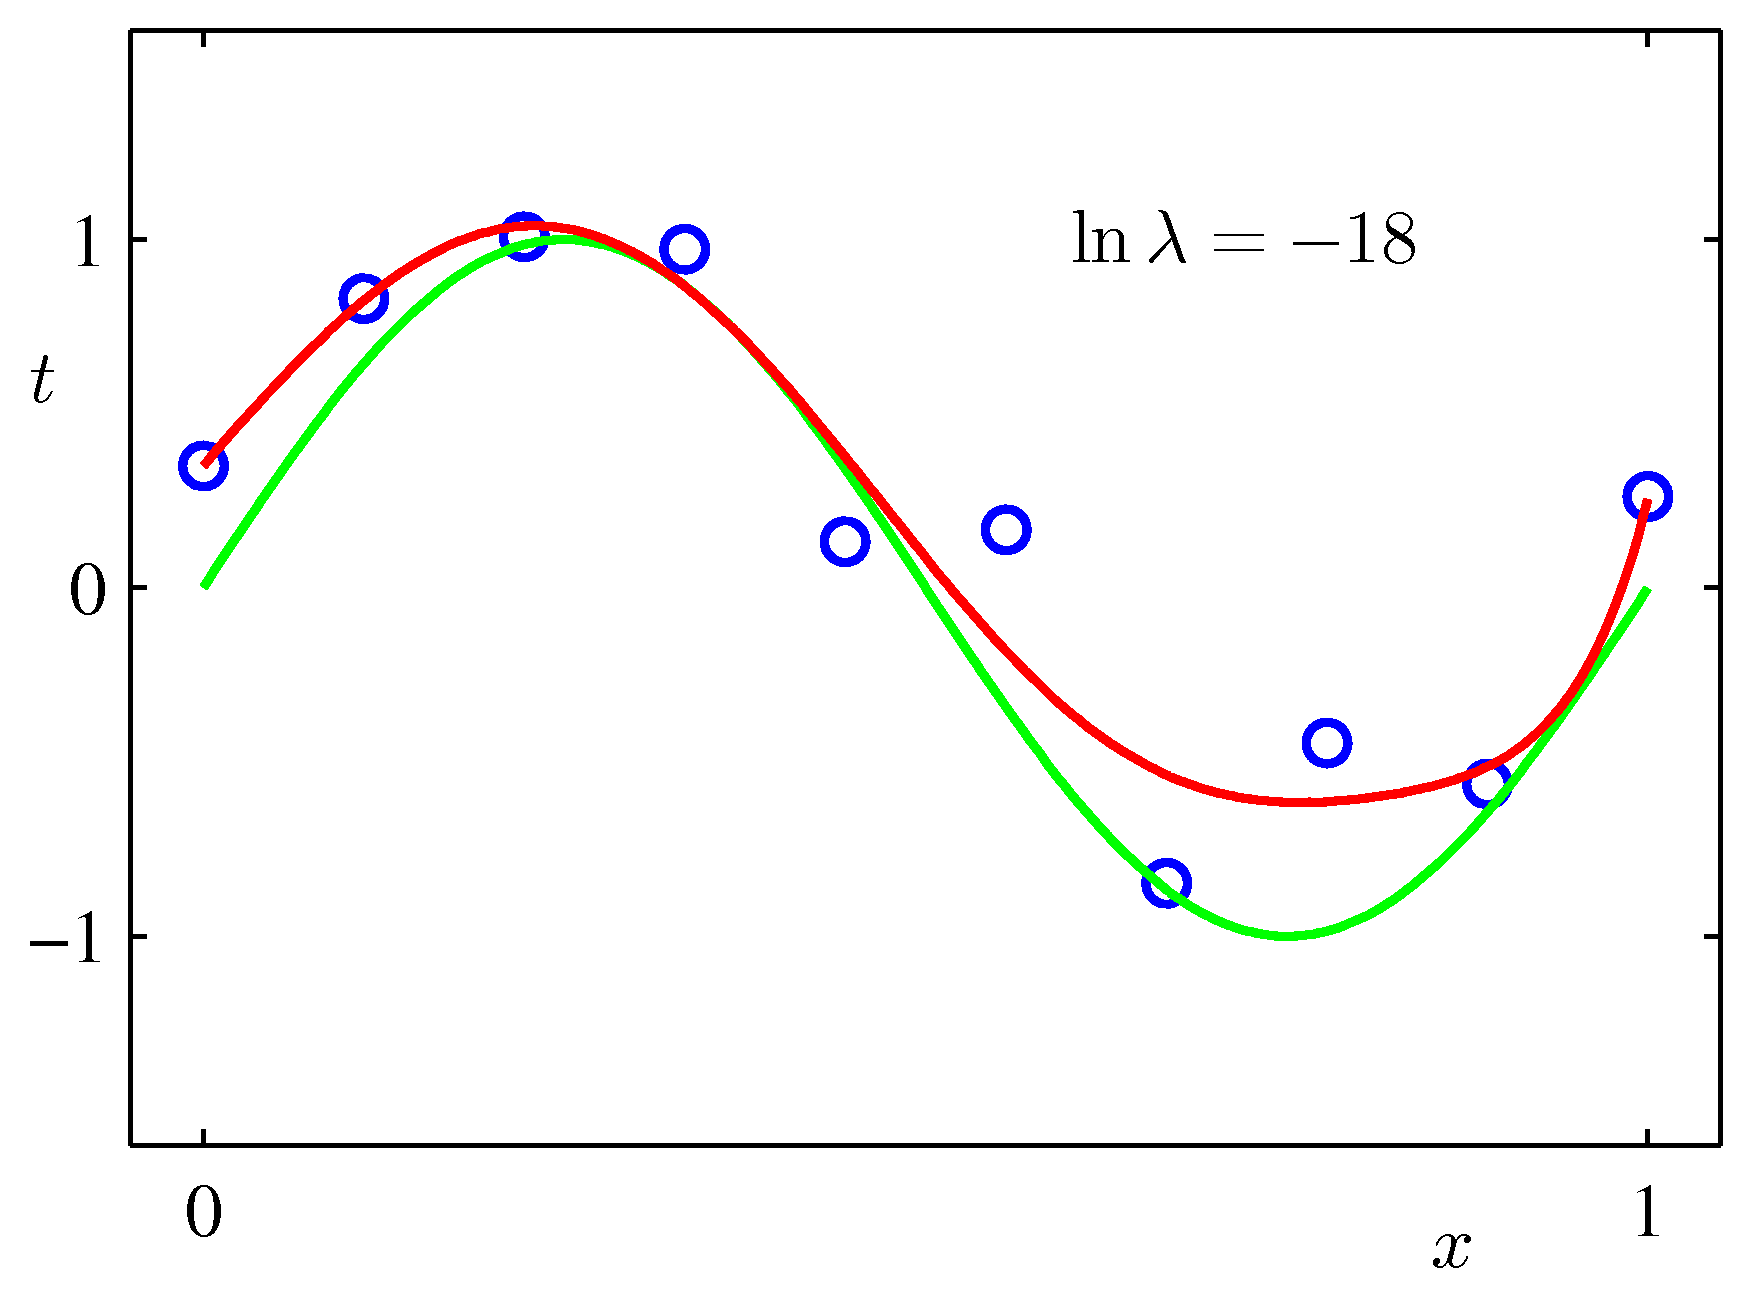
\includegraphics[scale=0.8]{Images/1-7a.png}
		\label{fig:1-7a}
		\end{minipage}
		\begin{minipage}[t]{0.5\linewidth}
		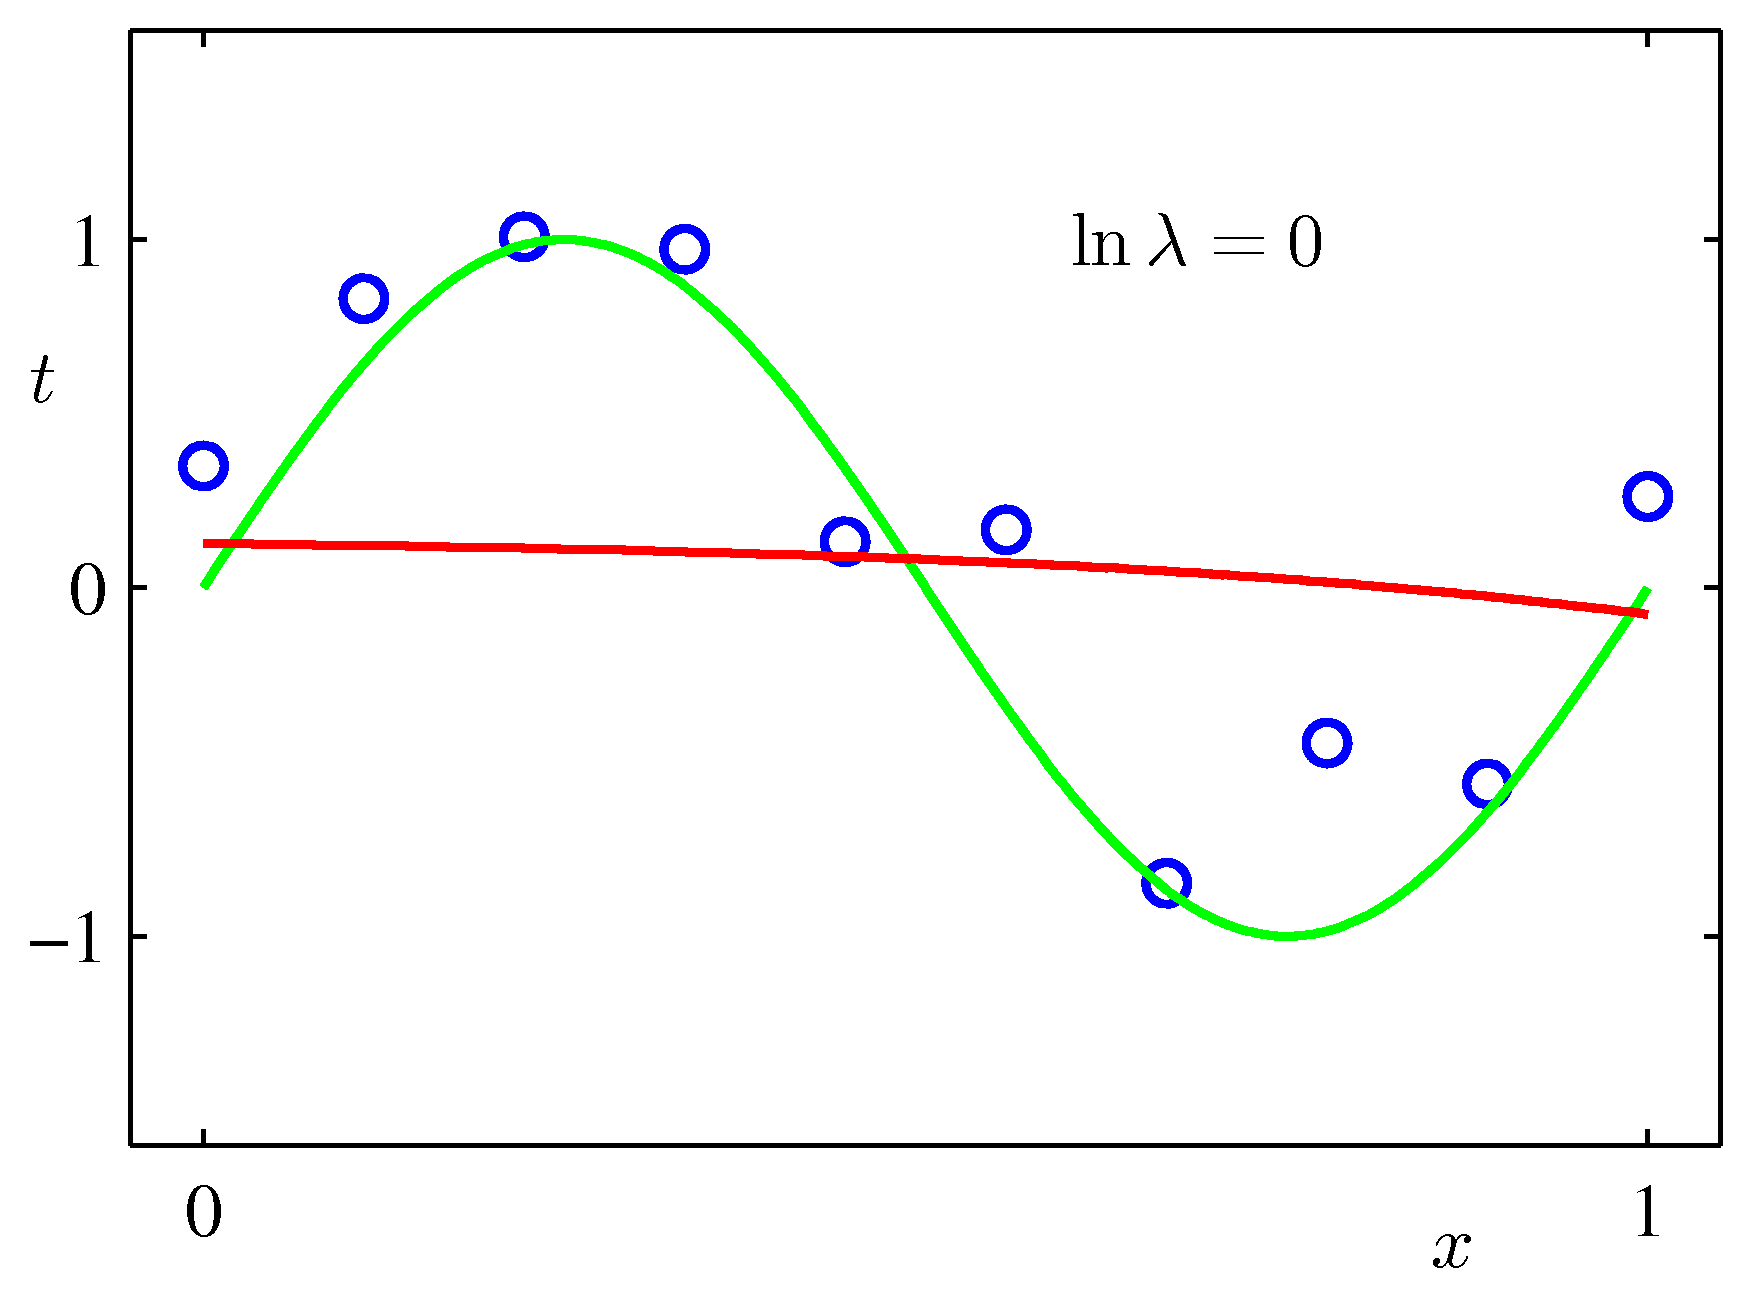
\includegraphics[scale=0.8]{Images/1-7b.png}
		\label{fig:1-7b}
		\end{minipage}
		\captionsetup{font={small}}
		\caption{在$M=9$的情况下,使用(1.4)中的正则化误差函数对图1.2所示的数据集进行拟合,并将正则化参数$\lambda$设置为$\ln \lambda = -18$和$\ln \lambda = 0$。没有正则化的情况(即$\lambda=0$,$\ln \lambda = -\infty$)如图1.4中的右下图所示。}
	\end{figure}
	\noindent 属性之一。\color{red} \textbf{——第3.4节} \color{black}通过使用贝叶斯(Bayesian)方法,可以有效地避免过拟合问题。我们将看到,即使参数数量超过数据点数量,也不会对贝叶斯观点在模型中的应用造成任何困难。其实在贝叶斯模型中,有效(effective)参数的数量将根据数据集的规模进行自发的调整。
	\indent 不过现在的工作也是有意义的,所以还是继续使用目前的方法,并研究如何在现实中将复杂且灵活的模型应用于规模有限的数据集。处理这种过拟合情况的一种常见方法是正则化(regularization),这种方法是在(1.2)中的误差函数里加入惩罚项,从而使系数不会达到太大的值。最简单的惩罚项是对所有系数取平方和,从而得到了如下经过修正的误差函数:
	\begin{equation}
		\widetilde{E}(\mathbf{w})=\frac{1}{2}\sum_{n=1}^{N} \{ y(x_n,\mathbf{w}) - t_n\}^2 + \frac{\lambda}{2} \| \mathbf{w} \|^2
	\end{equation}
	其中$\| \mathbf{w} \|^2 \equiv \mathbf{w^\mathrm{T} w} = w_0^2 + w_1^2 + ... + w_M^2$,系数$\lambda$控制的是正则项与平方和误差项相比之下的真实权重。需要注意的是,在正则式中系数$w_0$通常被省略,因为如果将它包含进来,可能会导致最终结果受到目标变量原点的影响(Hastie et al., 2001),如果要将其包含在内,该项就必须有自己的正则化系数(我们将在第5.5.1节中详细讨论这个话题)。与前面类似,(1.4)中的误差函数可以求取其最小化结果的解析解。\color{red} \textbf{——习题1.2} \color{black}由于系数的值变小了,所以诸如此类的技术在统计学中称为收缩(shrinkage)方法。这种二次正则器被称为岭回归(ridge regression, Hoerl and Kennard, 1970)。在神经网络中,这样的方法称为权重衰减(weight decay)。 \\
	\indent 图1.7展示了阶数$M=9$的多项式对相同数据集的拟合结果,只不过现在使用的误差函数是(1.4)中所示的带有正则项的误差函数。可以看出在$\ln \lambda = -18$时过拟合现象得到了有效的控制,我们得到了一个更加接近原函数$\sin (2 \pi x)$的拟合。但是如果将$\lambda$的值设得太大,我们又会得到一个很差的拟合结果,如图1.7中所示的是$\ln \lambda = 0$的情况。不同正则化参数对应的多项式系数拟合结果如表1.2所示,正则化有效地使多项式的系数变小了很多。\\
	\indent 在图1.8中,通过将训练集和测试集的RMS误差(1.3)各自与$\ln \lambda$的关系绘制在一起,可以看出正则项对泛化误差的影响。可以看出,现在参数$\lambda$有效控制了模型的复杂度,所以决定了过拟合的程度。\\
	\indent 模型复杂度是一个相当重要的问题,我们将在第1.3节中讨论。现在我们只简单地提一句,如果我们希望利用误差函数最小化的方法解决实际问题,就必须要找到一种能够确定合适的模型复杂度的方法。以上的结果算是提出了解决这一问题的一种简单方法,即通过将现有数据划分为训练集(用于确定系数$\mathbf{w^\star}$)和单独的验证集(validation set,亦称拿出集,hold-out set),用于模型复杂度的优化($M$或$\lambda$)。但在很多的场合中,这样的做法是对训练数据的浪费,我们需要寻求更加高级的方法。\color{red} \textbf{——第1.3节} \color{black}\\
	\begin{table}
		\centering
		\begin{tabular}{c|rrr}
			\ & $\ln \lambda = - \infty $ & $\ln \lambda = -18$ & $\ln \lambda = 0$ \\
			\hline
			$w_0^\star$ & 0.35 & 0.35 & 0.13 \\
			$w_1^\star$ & 232.37  & 4.74 & -0.05 \\
			$w_2^\star$ & -5321.83  & -0.77  & -0.06 \\
			$w_3^\star$ & 48568.31  & -31.97  & -0.05 \\
			$w_4^\star$ & -231639.30  & -3.89  & -0.03  \\
			$w_5^\star$ & 640042.26  & 55.28  & -0.02  \\
			$w_6^\star$ & -1061800.52  & 41.32  & -0.01  \\
			$w_7^\star$ & 1042400.18  & -45.95  & -0.00  \\
			$w_8^\star$ & -557682.99  & -91.53  & 0.00  \\
			$w_9^\star$ & 125201.43  & 72.68  & 0.01  \\
		\end{tabular}
		\captionsetup{font={small}}
		\caption{在$M=9$的情况下,不同的正则化参数$\lambda$对应的多项式系数$\mathbf{w^\star}$。需要注意的是,$\ln \lambda = - \infty$对应的是图1.4中所示的无正则化的模型。可以看到,随着$\lambda$的增大,系数的大小会随之减小。}
	\end{table}
	\begin{figure}[H]
		\centering
		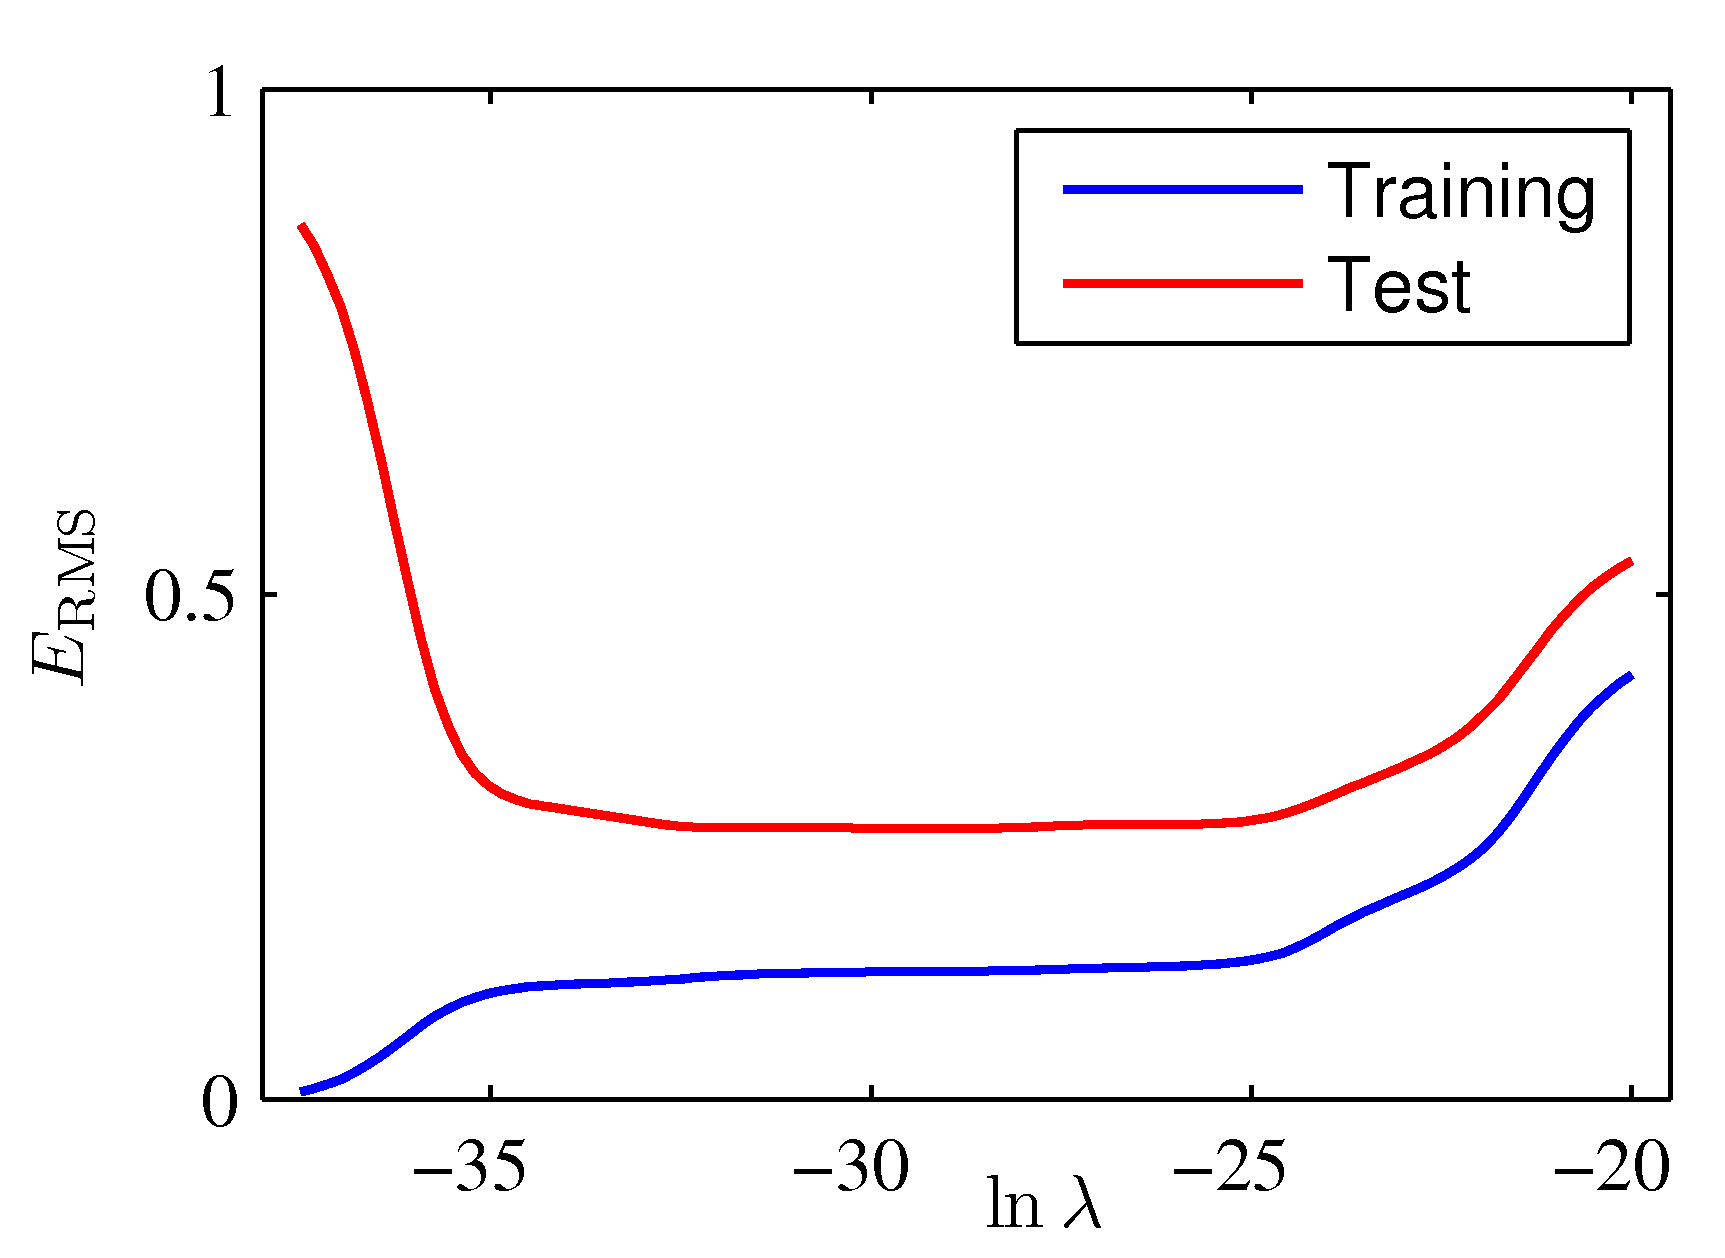
\includegraphics[scale=0.8]{Images/1-8.png}
		\captionsetup{font={small}}
		\caption{在$M=9$的情况下,均方根误差(1.3)随着$\ln \lambda$的变化情况。} 
		\label{fig:1-8}	
	\end{figure}
	到目前为止,关于多项式拟合的讨论很依赖于直觉。我们现在要用更加具体的方法来解决模式识别的问题,那就是概率论。概率论不仅为本书几乎所有的后续章节提供了基础,还能让我们更深刻地理解本章中我们通过多项式拟合的问题引出的重要概念,让我们能够把这些概念扩展到更复杂的情况。
	}
	\section{概率论}
	\noindent{\color{red} \rule[10pt]{\textwidth}{0.1em}}
	\textnormal{
	\indent 在模式识别领域中,最关键的概念之一就是不确定性。不确定性会随着观测噪声和数据集的规模而变化。概率论对于不确定性的量化和计算提供了一个合理的框架,并成为了模式识别的核心基础之一。将概率论与决策论(第1.5节)相结合,我们就可以利用现有的信息进行最优的预测,即使这些信息是不完整的或很含糊的也没关系。\\
	\indent 我们将通过一个简单的例子介绍概率论的一些基础概念。假设我们有两个箱子,一个是红色的,一个是蓝色的,在红色箱子里有2个苹果和6个橙子,在蓝色箱子里有3个苹果和1个橙子,如图1.9所示。假设现在要随机选择一个箱子,并从这个箱子中随机取出一个水果,观察一下是哪一种之后放回原来的箱子里。我们可以假想做了很多次实验。假设我们在40\%的情况下选择红色箱子,60\%的情况下选择蓝色箱子,从箱子中取出哪一个水果是完全等可能的。
	\begin{figure}[ht]
		\centering
		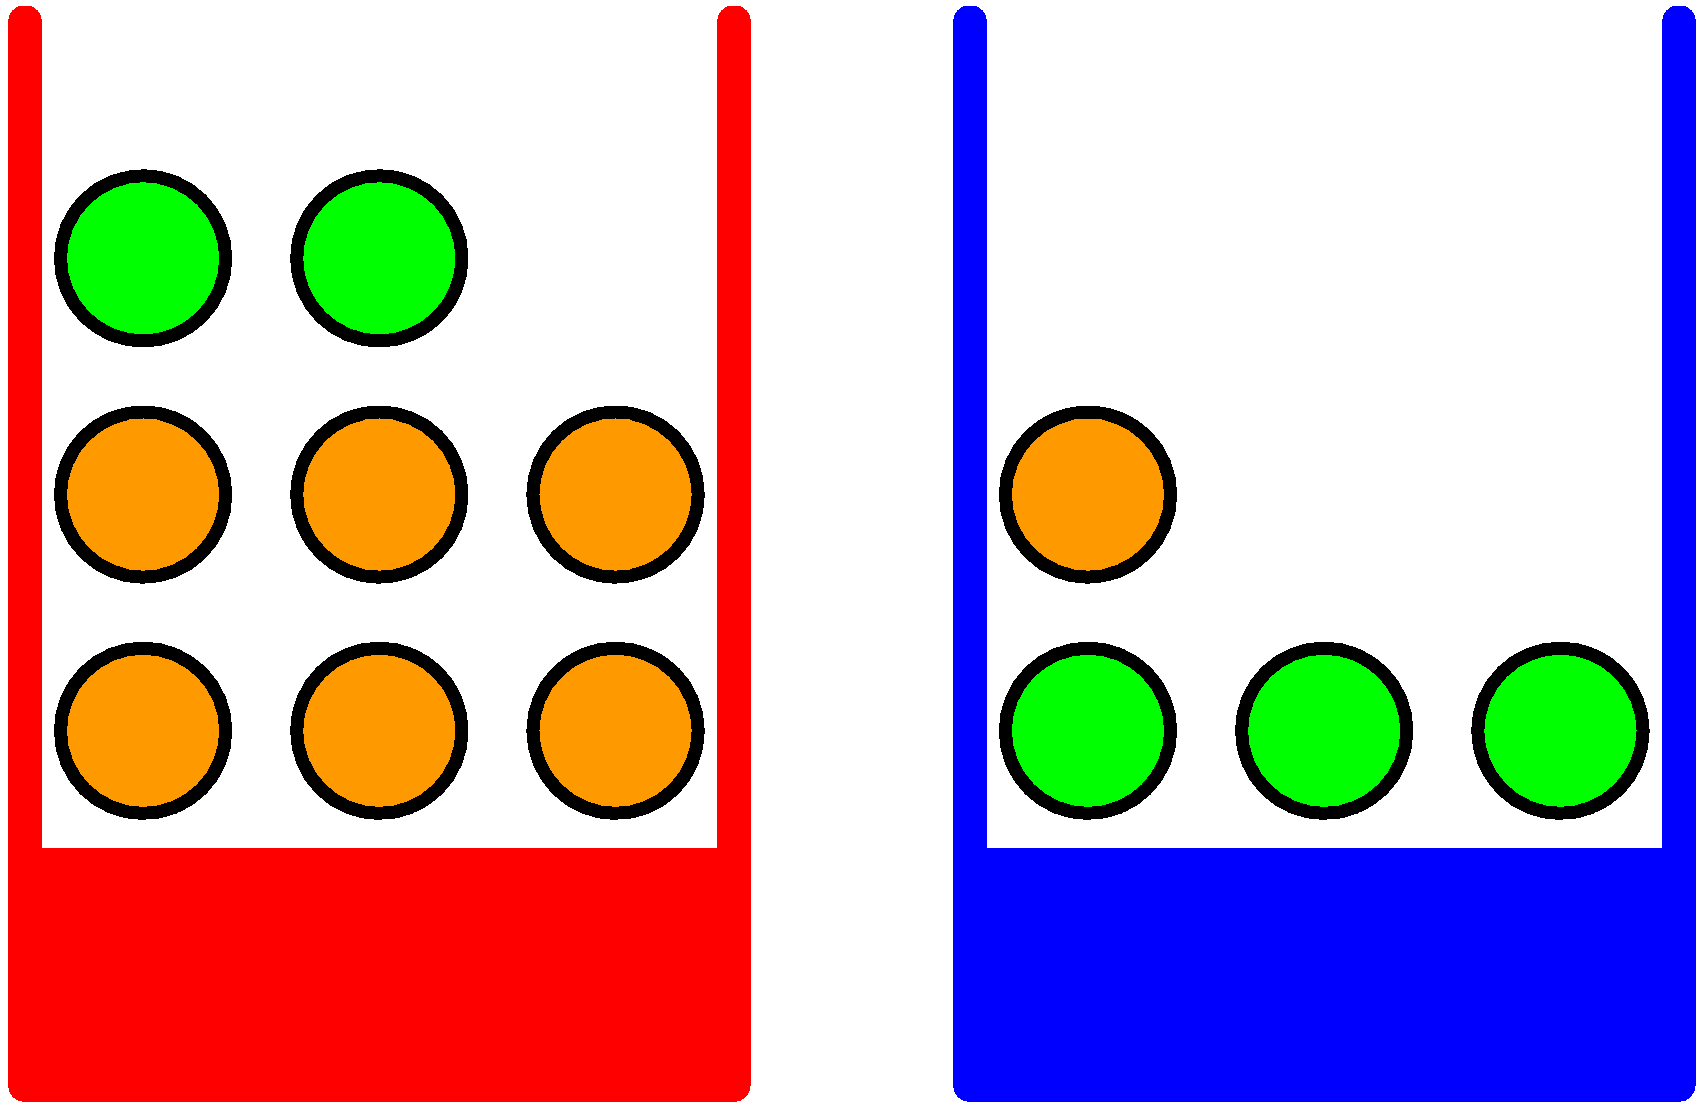
\includegraphics[scale=0.75]{Images/1-9.png}
		\captionsetup{font={small}}
		\caption{我们使用一个简单的小例子来介绍概率论的基础思想,图中是两个不同的箱子,箱子里放着不同类型的水果(绿色的是苹果,橙色的是橙子)。} 
		\label{fig:1-9}	
	\end{figure}
	\\
	\indent 在这个案例中,我们所选择的箱子的特性(颜色)是一个随机变量,记作$B$。这个随机变量有两种可能的取值,即$r$(红色)和$b$(蓝色)。类似地,所选择的水果的特性(种类)也是一个随机变量,记作$F$,其取值同样只有两种可能,即$a$(苹果)或$o$(橙子)。\\
	\indent 从概率的定义出发,我们将一个事件的概率定义为实验次数趋近于无穷时,事件发生的次数与实验总数的比值。于是,选择红色箱子的概率是4/10,选择蓝色箱子的概率是6/10。我们将其记作$p(B=r)=4/10$和$p(B=b)=6/10$。需要注意的是,根据定义,概率必须在区间$[0,1]$内。另外,如果某些事件是相互独立的,而且覆盖了所有可能的输出结果(例如,在这个例子中选择的箱子非红即蓝),那这些事件的概率之和一定等于1。\\
	\indent 现在我们可以问类似这样的问题:“拿到苹果的概率是多少?”或“已知拿到的是橙子,选择的箱子是蓝色箱子的概率是多少?”。这样的问题当然是可以解答的,比这复杂得多的模式识别问题都不在话下,不过首先要掌握加法规则(sum rule)和乘法规则(product rule)两项概率论基本规则。我们将在掌握这两项规则之后,再回到水果箱子案例中。\\
	\indent 为了推导概率中的这些规则,我们考虑一个稍微一般一些的情况,如图1.10所示,该例中包含了两个随机变量$X$和$Y$(类似于上一个例子中的箱子变量和水果变量)。假设$X$的取值可以是任意的$x_i$,其中$i=1,...,M$,$Y$的取值可以是任意的$y_j$,其中$j=1,...,L$。在$N$次实验中,对$X$和$Y$都进行了取样,并将$X=x_i,Y=y_j$的情况发生的次数记作$n_{ij}$。另外,将$X=x_i$的情况发生的次数(忽略$Y$的值)记作$c_i$,类似地将$Y=y_j$的情况发生的次数记作$r_j$。
	\begin{figure}[ht]
		\centering
		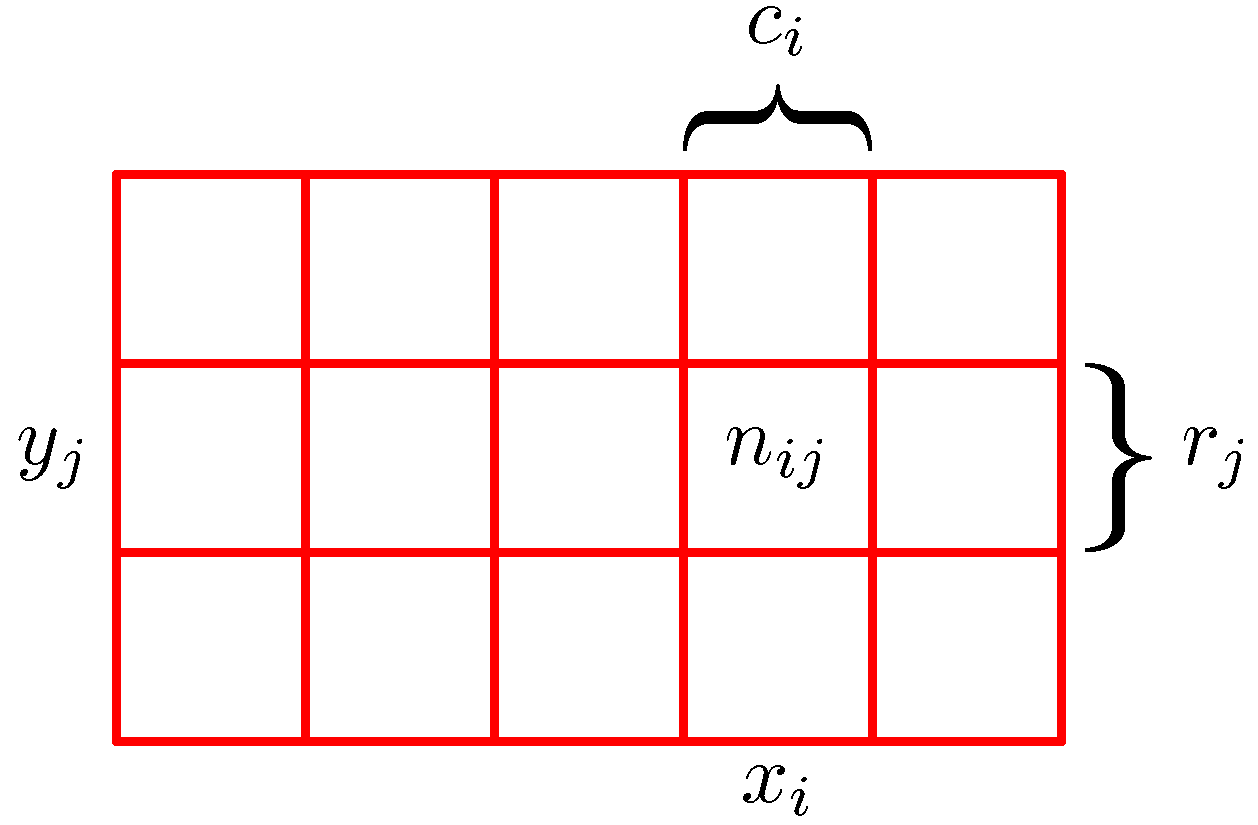
\includegraphics[scale=0.8]{Images/1-10.png}
		\captionsetup{font={small}}
		\caption{我们可以通过这样的例子来推导加法规则和乘法规则,有两个随机变量$X$和$Y$,其中$X$的取值范围是$\{x_i\},i=1,...,M$,$Y$的取值范围是$\{y_j\},j=1,...,L$。假设$M=5,L=3$,总共进行$N$次实验,将$X=x_i$且$Y=y_j$的次数记作$n_{ij}$,也就是落在相应单元格内的结果总数。在第$i$列中的点数对应的是$X=x_i$的情况发生的次数,记作$c_i$,在第$j$行中的点数对应的是$Y=y_j$的情况发生的次数,记作$r_j$。} 
		\label{fig:1-10}
	\end{figure}
	\\
	\indent $X=x_i$且$Y=y_j$的情况发生的概率称为$X=x_i$和$Y=y_j$的联合概率(joint probability),记作$p(X=x_i,Y=y_j)$。联合概率由落入$(i,j)$单元格中的结果数量与总实验次数求取比值得到,即:
	\begin{equation}
		p(X=x_i,Y=y_j)=\frac{n_{ij}}{N}
	\end{equation}
	\indent 在这里我们比较隐晦地认为$N$是趋近于无穷的。类似地,既然$X=x_i$的概率是与$Y$的取值无关的,所以就是第$i$列中的结果总数与实验总数的比值,那么$p(X=x_i)$就可以写成:
	\begin{equation}
		p(X=x_i)=\frac{c_i}{N}
	\end{equation}
	\indent 由于图1.10中第$i$列中的结果总数就是该列中每一个单元格里结果数的总和,于是有$c_i=\sum_{j}n_{ij}$,所以根据(1.5)和(1.6),可以得到:
	\begin{equation}
		p(X=x_i)=\sum_{j=1}^{L} p(X=x_i,Y=y_j)
	\end{equation}
	\indent 这就是概率的加法规则。需要注意的是,有时$p(X=x_i)$被称为边缘概率(marginal probability),因为它是通过将其他变量(在这个例子中是$Y$)进行边缘化(或者说求和)得到的。\\
	\indent 如果仅考虑$X=x_i$的情况,在这样的限制下$Y=y_j$的结果数在$X=x_i$的结果中所占的比例被称为给定$X=x_i$的$Y=y_j$的条件概率(conditional probability),记作$p(Y=y_j|X=x_i)$。条件概率要通过计算$(i,j)$单元格中的结果数与第$i$列中的结果总数的比值得到,即:
	\begin{equation}
		p(Y=y_j|X=x_i)=\frac{n_{ij}}{c_i}
	\end{equation}
	\indent 根据(1.5),(1.6)和(1.8),我们可以进行如下推导:
	\begin{equation}
		p(X=x_i,Y=y_j) = \frac{n_{ij}}{N}=\frac{n_{ij}}{c_i} \cdot \frac{c_i}{N} = p(Y=y_j|X=x_i)p(X=x_i)
	\end{equation}
	\indent 这就是概率的乘法规则。\\
	\indent 到目前为止我们一直都比较小心地将随机变量(比如水果箱子案例中的箱子变量$B$)和随机变量可能的取值(比如$B=r$)区分开来。所以,$B$的取值为$r$的概率可以记为$p(B=r)$。尽管这样讲可以避免歧义,但真的很是繁琐,而且很多情况下确实不需要这样刻板。所以我们不用这样的写法,而是将随机变量$B$的分布记作$p(B)$,将该分布取特定值$r$的估计记作$p(r)$,这样就清楚得多了。\\
	\indent 有了这样更加简练的表示,我们可以将概率论的两条基本规则写成如下的形式:\\
	\insertline\\
	\color{red} $\bullet$ \textbf{\ 概率论的基本规则} \color{black}
	\begin{align}
		\textbf{加法规则(sum rule)\ \ \ \ } &p(X)=\sum_{Y}^{}p(X,Y) \\
		\textbf{乘法规则(product rule)\ \ \ \ } &p(X,Y)=p(Y|X)p(X)
	\end{align}
	\insertline\\
	\indent 这里的$p(X,Y)$表示的是联合概率,也就是“$X$且$Y$的概率”。类似地,$p(Y|X)$表示的是条件概率,也就是“在$X$的情况下$Y$的概率”,$p(X)$为边缘概率,也就是“$X$的概率”。这两项基础规则构成了概率论的基础,会在本书中贯穿始终。\\
	\indent 从乘法规则出发并引入对称性$p(X,Y)=p(Y,X)$,我们马上就可以得到条件概率之间的如下关系:
	\begin{equation}
		p(Y|X)=\frac{p(X|Y)p(Y)}{p(X)}
	\end{equation}
	\indent 这就是著名的贝叶斯定理(Bayes' theorem),它在模式识别和机器学习中扮演了核心的角色。利用加法规则,贝叶斯定理中的分母可以表示为:
	\begin{equation}
		p(X)=\sum_{Y}^{} p(X|Y)p(Y)
	\end{equation}
	\indent 可以看出贝叶斯定理中的分母其实是一个归一化常数,保证了(1.12)等式左侧满足$Y$的全部取值的条件概率之和为1。\\
	\indent 在图1.11中,我们展示了一个包含两个变量的联合分布的案例来解释边缘分布(marginal distribution)和条件分布(conditional distribution)的概念。其中,左上方的图展示了一个从联合分布中抽取的包含有$N=60$个数据点的有限样本。右上方的直方图展示了两种取值的$Y$各自所占的比例。根据概率的定义,在$N\rightarrow \infty$时,该比例将等于其相应的概率。我们可以将直方图视作在给定了从分布中抽取的有限点的情况下,模拟概率分布的一种简单方法。通过数据对分布进行建模是统计模式识别的核心,在本书中将进行详细的探讨。图1.11中余下的两个图展示了$p(X)$和$p(X|Y=1)$的直方图估计。
	\begin{figure}[ht]
		\begin{minipage}[t]{0.5\linewidth}
		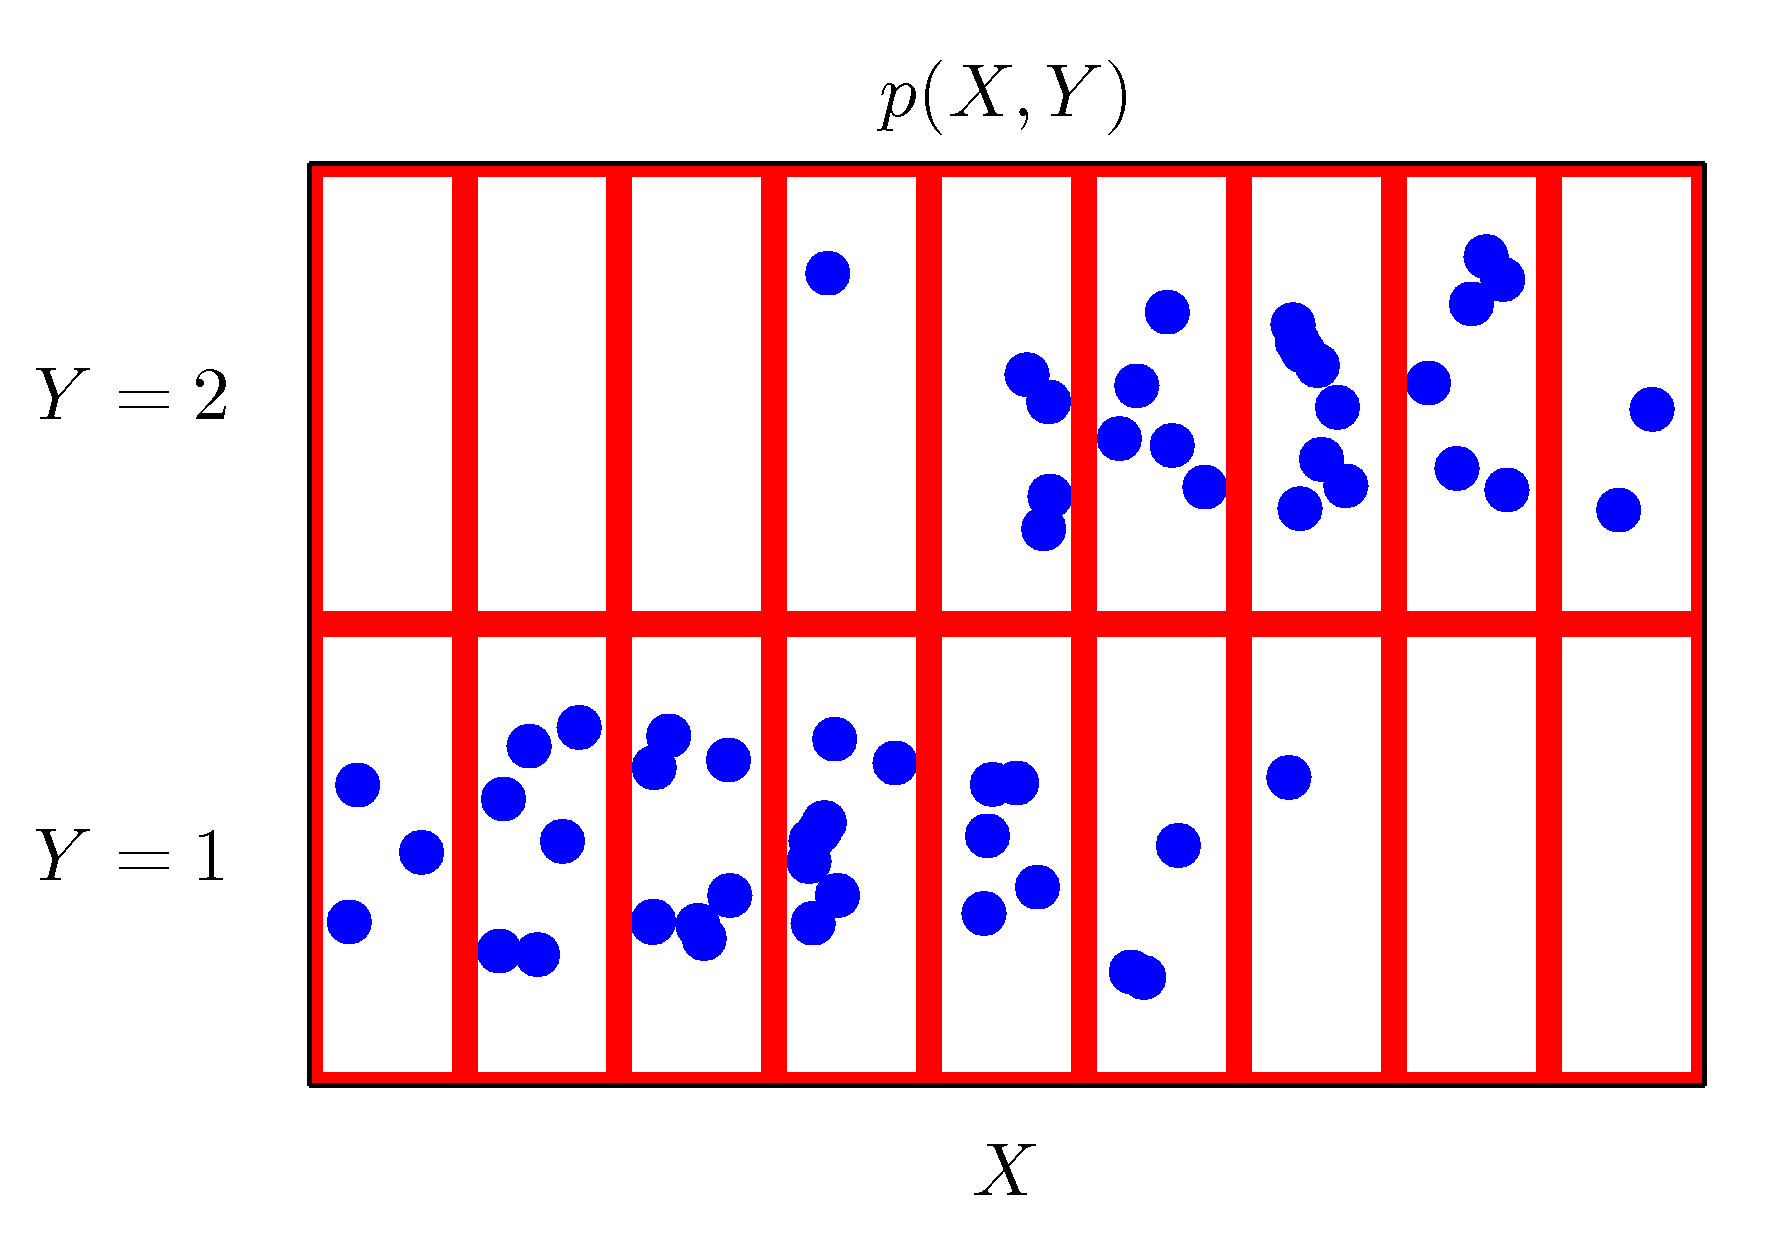
\includegraphics[scale=0.8]{Images/1-11a.png}
		\label{fig:1-11a}
		\end{minipage}
		\begin{minipage}[t]{0.5\linewidth}
		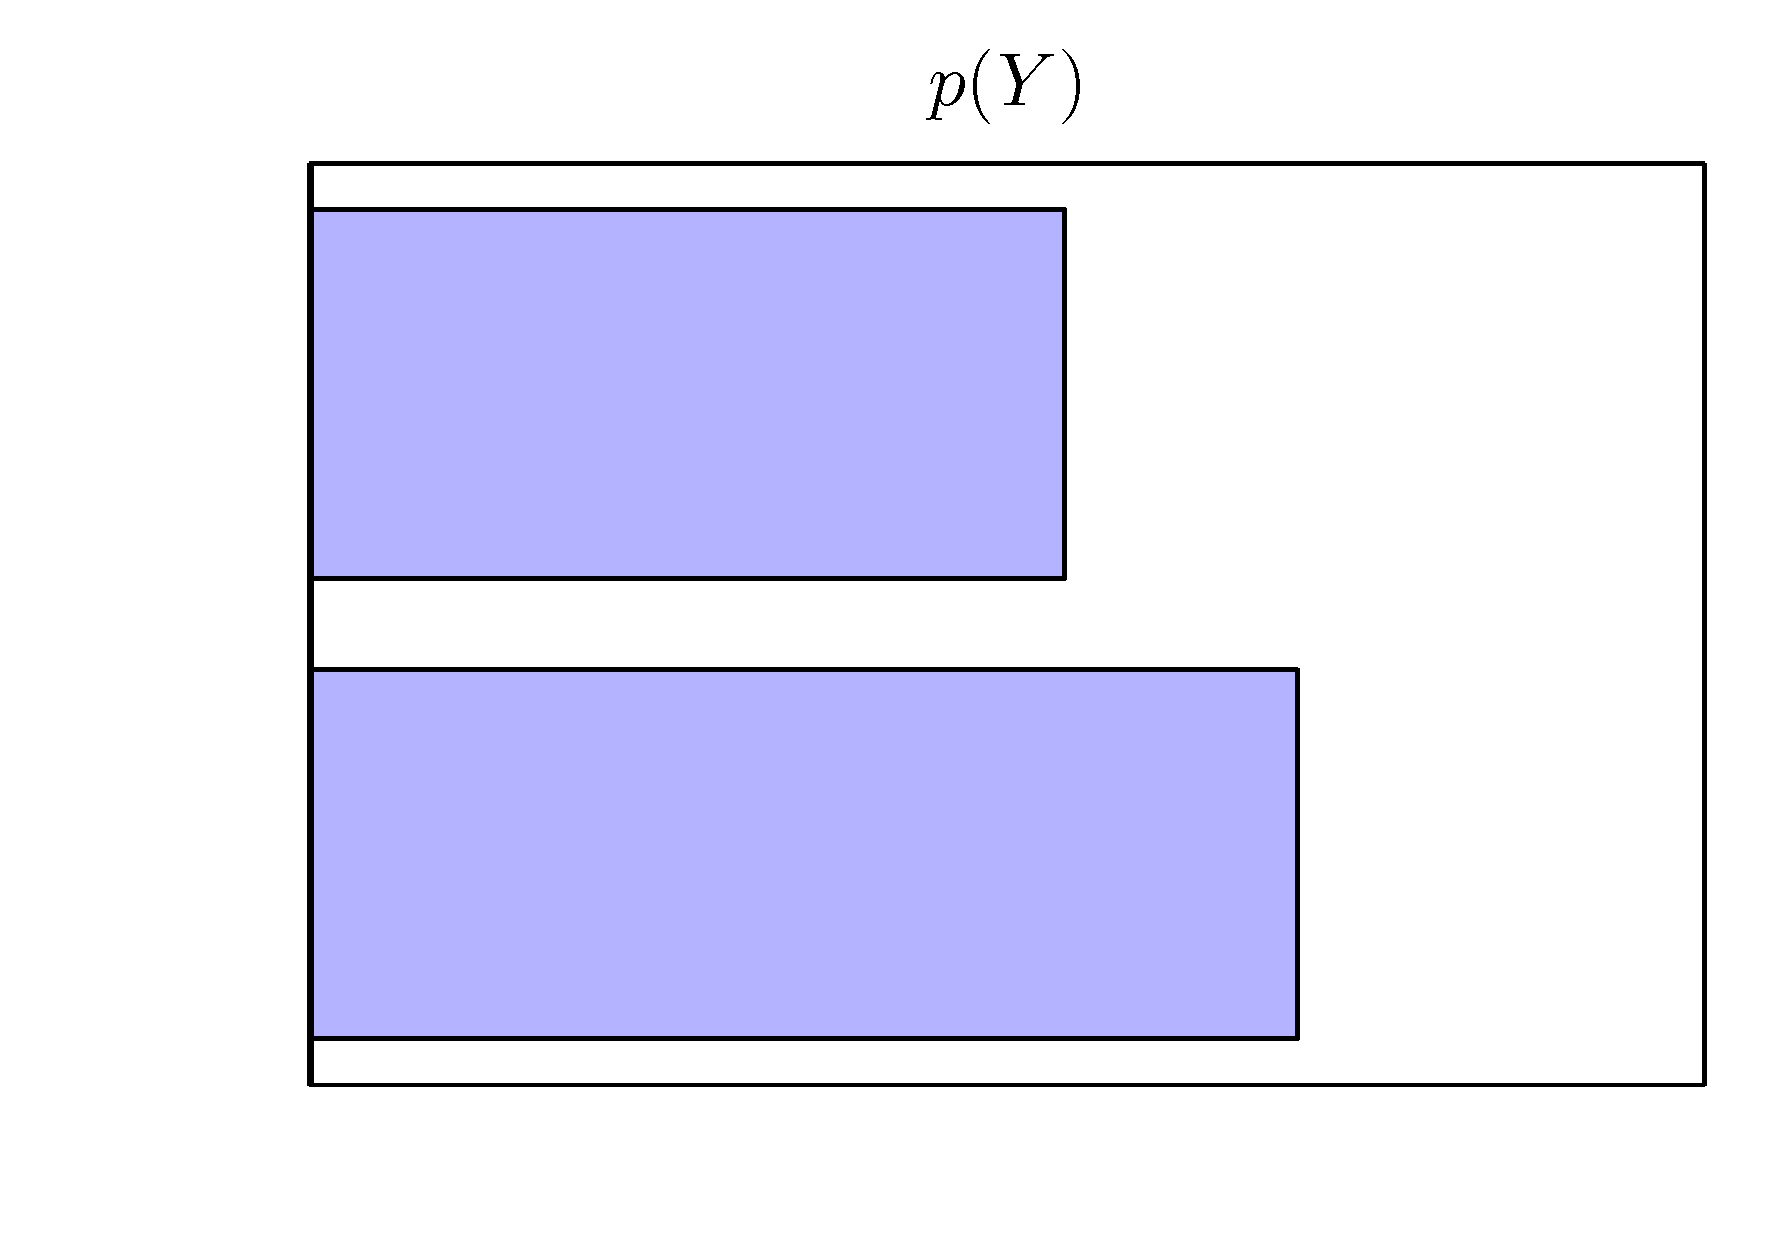
\includegraphics[scale=0.8]{Images/1-11b.png}
		\label{fig:1-11b}
		\end{minipage}\\
		\begin{minipage}[t]{0.5\linewidth}
		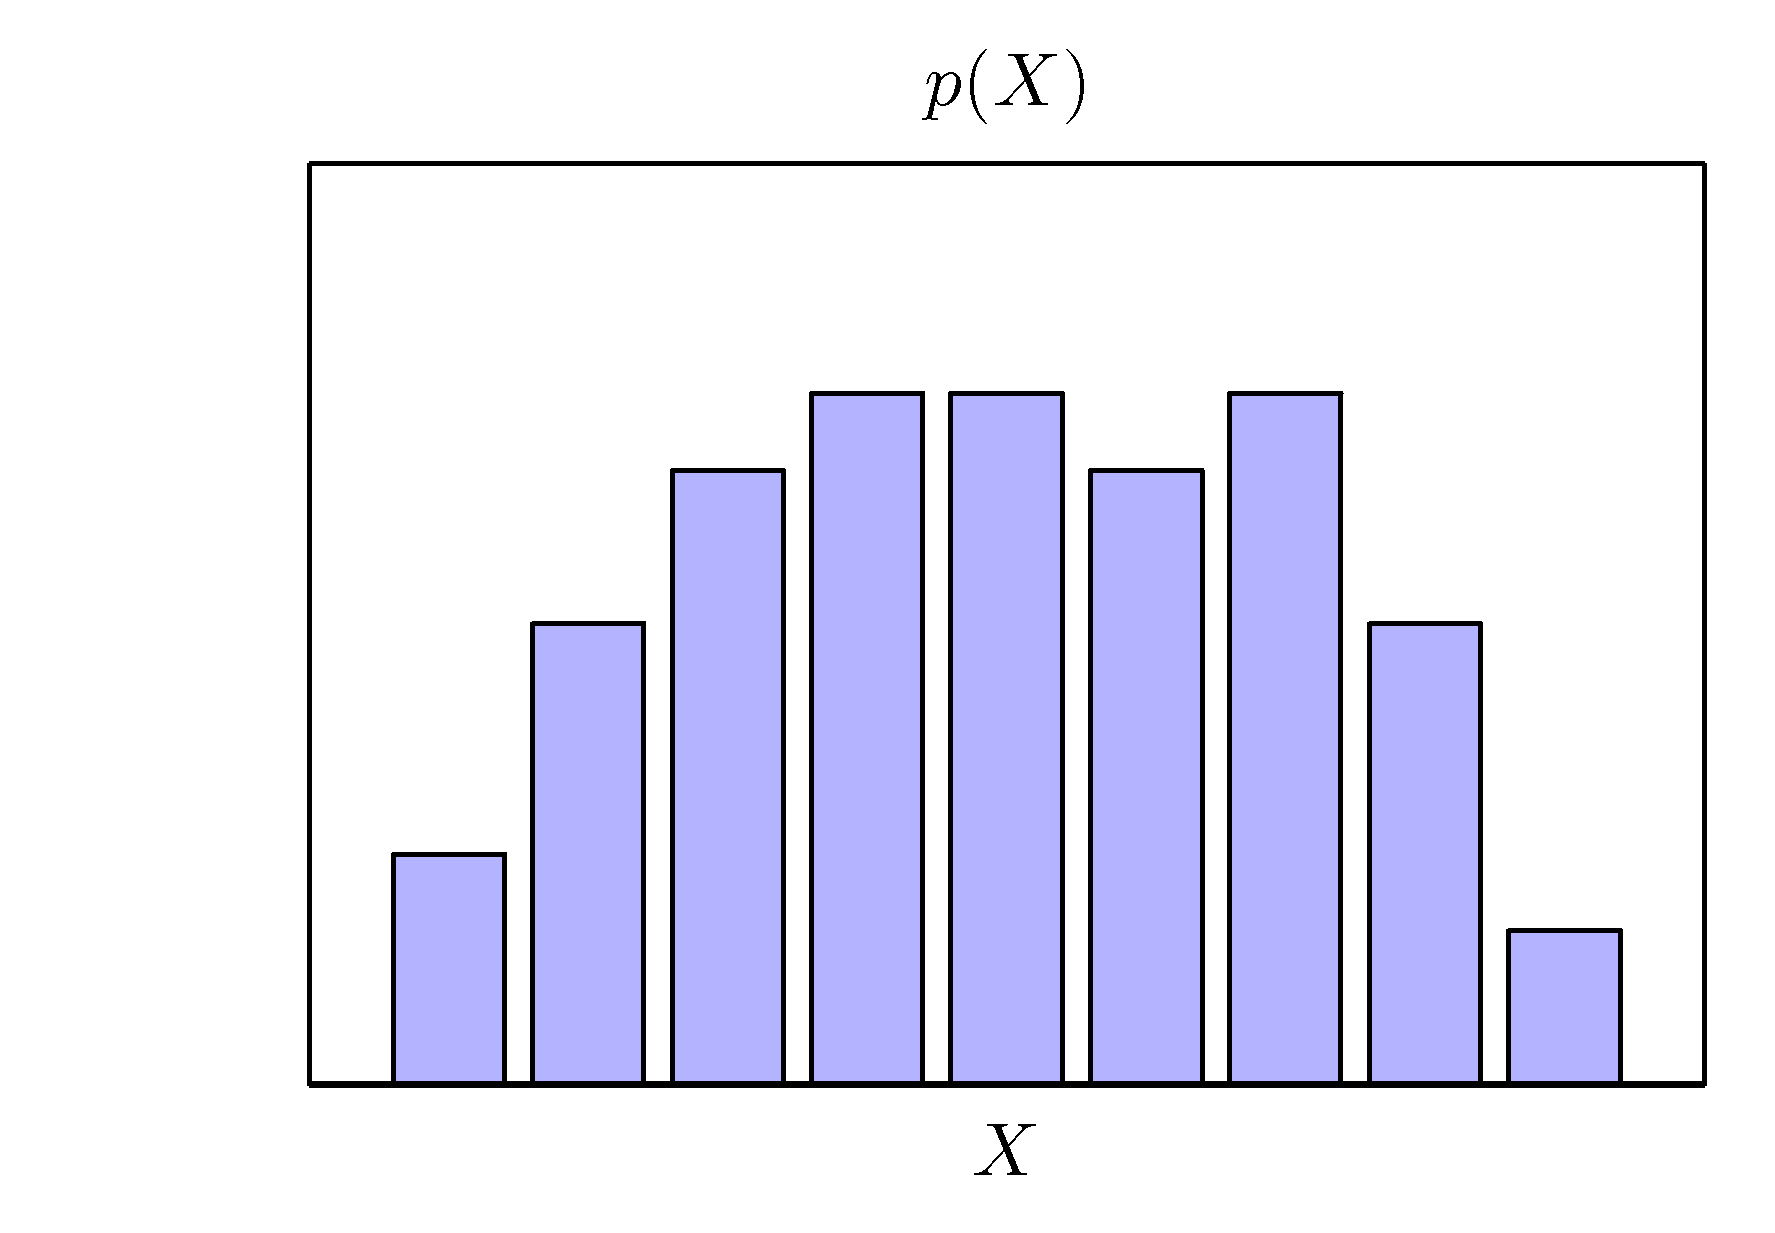
\includegraphics[scale=0.8]{Images/1-11c.png}
		\label{fig:1-11c}
		\end{minipage}
		\begin{minipage}[t]{0.5\linewidth}
		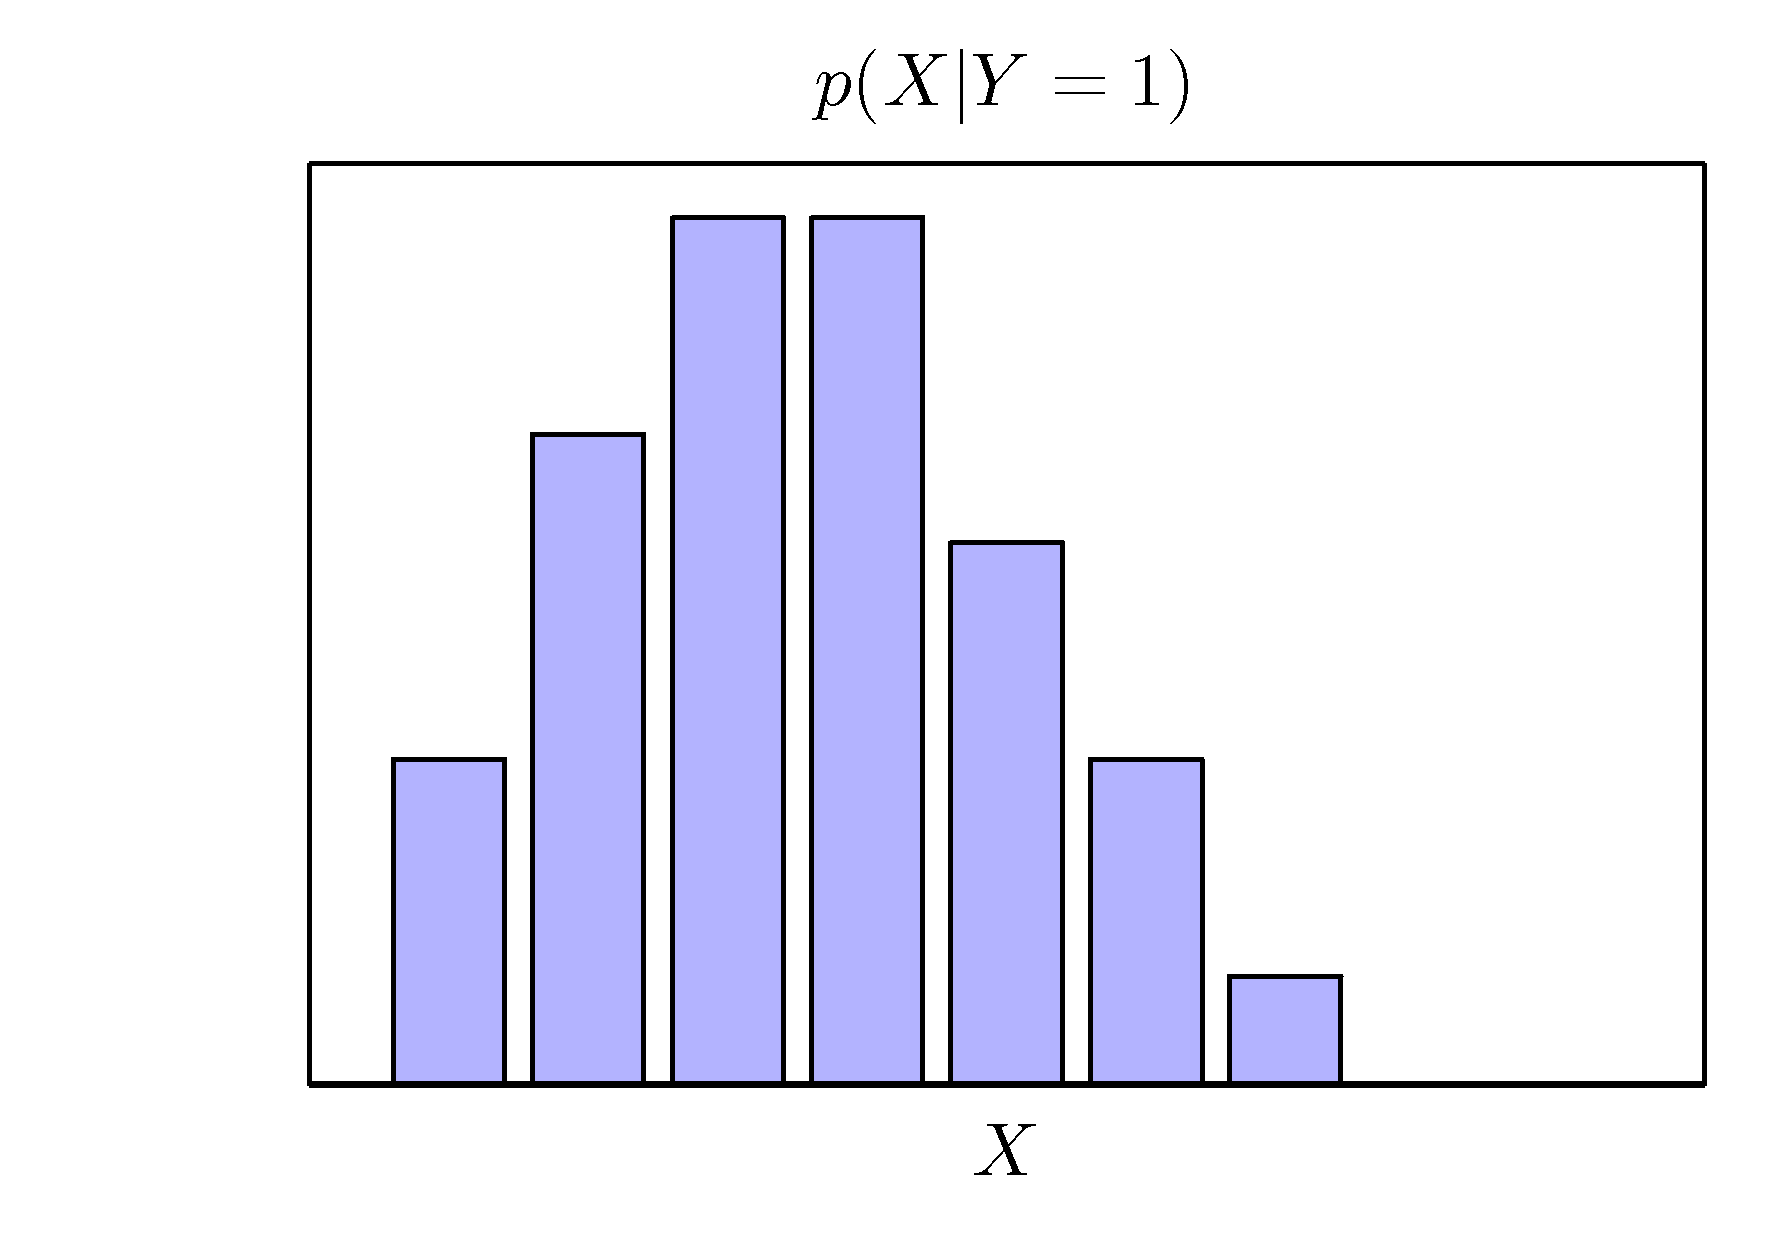
\includegraphics[scale=0.8]{Images/1-11d.png}
		\label{fig:1-11d}
		\end{minipage}
		\captionsetup{font={small}}
		\caption{两个变量的分布图,$X$有9种可能的取值,$Y$有2种可能的取值。左上图显示了从这些变量的联合概率分布中抽取的60个样本点。其余图显示了边缘分布$p(X)$和$p(Y)$的直方图估计,以及对应于左上图中下面一行的条件分布$p(X|Y=1)$。}
	\end{figure}
	\\
	\indent 现在我们回到之前的水果箱子案例中,再次对随机变量与其取值进行区分。选择红色箱子和蓝色箱子的概率分别为:
	\begin{align}
		p(B=r)&=4/10 \\
		p(B=b)&=6/10
	\end{align}
	\indent 注意,$p(B=r)+p(B=b)=1$。\\
	\indent 假设我们随机选择了一个箱子,发现是蓝色的。那么选择到苹果的概率就是蓝色箱子中苹果的比例,即3/4,也就是说$p(F=a|B=b)=3/4$。事实上,我们可以写出给定箱子的情况下,取出水果种类的全部四种概率:
	\begin{align}
		p(F=a|B=r) &=1/4 \\
		p(F=o|B=r) &=3/4 \\
		p(F=a|B=b) &=3/4 
	\end{align}
	\begin{equation}
		p(F=o|B=b) =1/4 
	\end{equation}
	\indent 概率在这里同样是归一化的:
	\begin{align}
		p(F=a|B=r)+p(F=o|B=r) &=1 \\
		p(F=a|B=b)+p(F=o|B=b) &=1
	\end{align}
	\indent 于是我们可以利用加法规则和乘法规则计算完整的取出苹果的概率:
	\begin{equation}
		\begin{split}
			p(F=a) &= p(F=a|B=r)p(B=r)+p(F=a|B=b)p(B=b) \\ 
			&= \frac{1}{4}\times\frac{4}{10}+\frac{3}{4}\times\frac{6}{10} = \frac{11}{20}
		\end{split}
	\end{equation}
	\indent 于是$p(F=o)=1-11/20 = 9/20$。\\
	\indent 假设现在换一种情况,我们已知的是拿到的水果是一个橙子,希望知道是从哪一个箱子里拿出的水果。这就要求我们估计给定水果类别情况下的箱子类别的概率分布,相比之下,(1.16)~(1.19)给出的是给定箱子类别的情况下水果类别的概率分布。我们可以利用贝叶斯定理来求解这个问题:
	\begin{equation}
		p(B=r|F=o)=\frac{p(F=o|B=r)p(B=r)}{p(F=o)}=\frac{3}{4} \times \frac{4}{10} \times \frac{20}{9} = \frac{2}{3}
	\end{equation}
	\indent 根据加法规则,$p(B=b|F=o)=1-2/3=1/3$。\\
	\indent 我们可以给出对于贝叶斯定理的如下重要解释。如果我们要在知晓拿到的水果种类之前预测箱子的类别,那么我们可以利用的最完整的信息来自于$p(B)$。我们将之称为\textbf{先验概率}(prior probability),因为这一项概率是在我们得到水果类别之前就可以获得的。一旦我们被告知了水果的类别(比如说橙子),我们就可以用贝叶斯定理去求取$p(B|F)$,这一项我们称为\textbf{后验概率}(posterior probability),因为我们会在得到$F$之后得到这一概率。注意在这个案例中,选择红色箱子的先验概率是4/10,所以选择蓝色箱子的可能性要大于红色箱子。但是,一旦我们观测到了取出的水果是一个橙子,选择红色箱子的后验概率就是2/3了,所以选择红色箱子的可能性就更大了。这个结果是比较符合我们的直觉的,因为红色箱子中橙子的比例要远大于蓝色箱子的,所以拿出的水果是橙子这一事件为做出选择的箱子是红色箱子这一预测提供了很有利的判据。其实,这项判据强大到以至于盖过了先验,使得选择的箱子更有可能是红色箱子而非蓝色箱子。\\
	\indent 最后,还要注意到,如果两个变量的联合分布可以分解为两个边缘分布的乘积,即$p(X,Y)=p(X)p(Y)$,那么$X$和$Y$就是相互独立的(independent)。根据乘法规则,$p(Y|X)=p(Y)$,所以给定$X$的$Y$的条件分布是完全独立于$X$的。例如,在水果箱子案例中,如果每个箱子中包含相同比例的苹果和橙子,那么$p(F|B)=p(F)$,那么选择出的水果是苹果的概率就独立于选择的箱子的类别。}
	\subsection{概率密度}
	\textnormal{研究离散事件集合的概率的同时,我们还要考虑连续变量的概率。对此的讨论将仅限于相对非正式的形式。如果一个实值变量$x$落在区间$(x,x+\delta x)$中的概率由$p(x)\delta x , \delta x \rightarrow 0$ 给出,那么$p(x)$就被称为$x$的\textbf{概率密度}(probability density)。图1.12对此做出了解释。$x$落在区间$(a,b)$中的概率由以下公式给出:
	\begin{equation}
		p(x\in(a,b))=\int_{a}^{b}p(x)\ \mathrm{d}x
	\end{equation}
	\begin{figure}[ht]
		\centering
		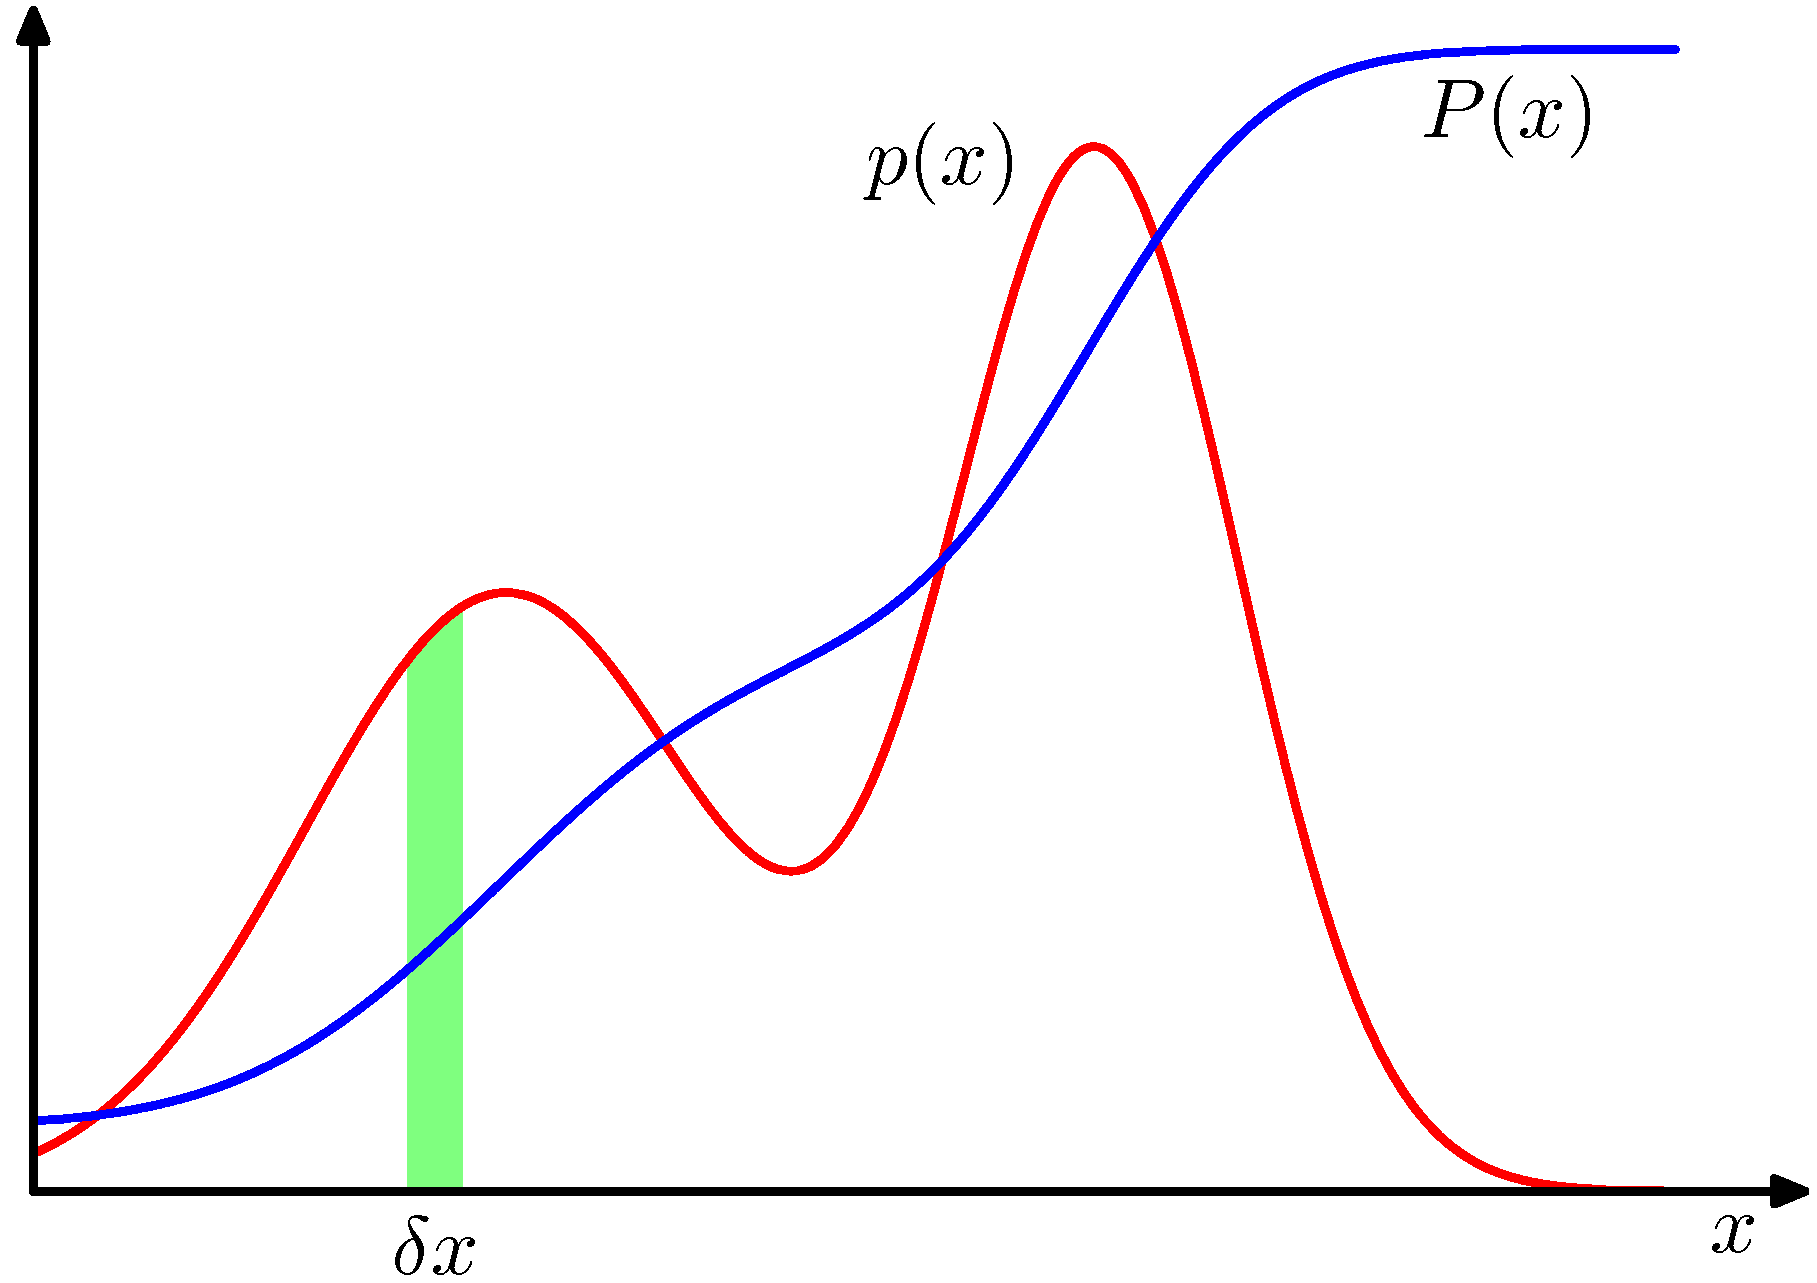
\includegraphics[scale=0.8]{Images/1-12.png}
		\captionsetup{font={small}}
		\caption{离散变量的概率可以扩展为连续变量$x$的概率密度$p(x)$,于是$x$的取值落在区间$(x,x+\delta x)$中的概率由$p(x)\delta x , \delta x \rightarrow 0$给出。概率密度可以被表示为累积分布函数(即分布函数,cumulative distribution function)的导数。} 
		\label{fig:1-12}	
	\end{figure}
	\\
	\indent 由于概率是非负的,而且$x$的值一定是在实轴范围内的,所以概率密度$p(x)$一定满足如下条件:
	\begin{align}
		p(x) &\geqslant 0 \\
		\int_{-\infty}^{+\infty}p(x)\ \mathrm{d}x &= 1
	\end{align}
	\indent 在变量的非线性变换下,由于雅可比因子(Jacobian factor),概率密度的变换与一般的函数不同。举例而言,假设有一个变量的变换$x=g(y)$,那么函数$f(x)$就变成了$\widetilde{f}(y)=f(g(y))$。接下来我们探讨一个概率密度函数$p_x(x)$,与它对应的是关于新变量的概率密度$p_y(y)$,这里使用了不同的下标来表示$p_x(x)$和$p_y(y)$是两个不同的概率密度。对于很小的$\delta x$,落在区间$(x,x+\delta x)$的结果将变换到$(y,y+\delta y)$中,且有$p_x(x)\delta x\approx p_y(y)\delta y$,于是
	\begin{equation}
		\begin{split}
			p_y(y)&=p_x(x)\left|\frac{\mathrm{d}x}{\mathrm{d}y}\right|\\
			&=p_x(x)(g(y))\left| g'(y) \right|
		\end{split}
	\end{equation}
	\indent 这个性质导致的结果之一是,概率密度的最大值取决于变量的选择。\color{red}\textbf{——习题1.4}\color{black}\\
	\indent $x$的取值落在区间$(-\infty,z)$中的概率由累积分布函数(cumulative distribution function)给出:
	\begin{equation}
		P(z)=\int_{-\infty}^{z}p(x)\ \mathrm{d}x
	\end{equation}
	\indent 很明显$P'(x)=p(x)$,如图1.12所示。\\
	\indent 如果有多个连续变量$x_1,...,x_D$,且将其合并记作向量$\mathbf{x}$,那么就可以定义一个联合概率密度$p(\mathbf{x})=p(x_1,...,x_D)$,这样$\mathbf{x}$落在一个无穷小体积$\delta \mathbf{x}$(其中包含了$\mathbf{x}$点)中的概率就可以表示为$p(\mathbf{x})\delta x$。多元概率密度一定满足:
	\begin{align}
		p(\mathbf{x}) &\geqslant 0 \\
		\int p(\mathbf{x})\  \mathrm{d} \mathbf{x} &= 1
	\end{align}
	\indent 其中的积分是在整个$\mathbf{x}$空间上的。此外我们还可以考虑离散变量和连续变量的联合概率分布。\\
	\indent 注意,如果$x$是一个离散变量,那么$p(x)$有时也被称为概率质量函数(probability mass function),因为可以看作是集中在可能的$x$取值处的“概率质量”的集合。\\
	\indent 加法规则、乘法规则和贝叶斯定理同样适用于概率密度,以及离散变量与连续变量联合的情况。举例而言,如果$x$和$y$是两个实值变量,那么加法规则和乘法规则有如下形式:
	\begin{align}
		p(x)&=\int p(x,y) \ \mathrm{d} y \\
		p(x,y)&=p(y|x)p(x)
	\end{align}
	正式地证明连续变量的加法规则和乘法规则(Feller,1966)需要使用大量测度论(measure theory)的内容,这远远超出了本书的范围。然而,通过将每个实变量划分成宽度为$\Delta$的区间,并考虑在这些区间上的离散概率分布,可以不太正式地看出这一做法的合理性。令$\Delta \rightarrow 0$,则可以将求和转化为积分,并给出一个确切的结果。
	}
	\subsection{期望与协方差}
	\textnormal{涉及到概率的最重要的运算之一就是寻找函数的加权平均值。函数$f(x)$在概率分布$p(x)$下的平均值被称为函数$f(x)$的期望(expectation),记作$\mathbb{E}[f]$。对于离散分布:
	\begin{equation}
		\mathbb{E}[f]=\sum_{x}^{} p(x)f(x)
	\end{equation}
	\indent 于是这个平均值由不同的$x$值对应的概率赋予了权值。对于连续变量的情况,期望是由对概率密度积分的形式表达的:
	\begin{equation}
		\mathbb{E}[f]=\int p(x)f(x)\ \mathrm{d}x
	\end{equation}
	\indent 无论是哪一种情况,如果从概率分布或概率密度中提取了有限的$N$个点,那么就可以利用这些点来估计期望:
	\begin{equation}
		\mathbb{E}[f] \approx \frac{1}{N}\sum_{n=1}^{N}f(x_n)
	\end{equation}
	\indent 我们将在第11章中对取样方法进行讨论时经常用到这个结论。在$N \rightarrow \infty$时,(1.35)中的估计将会变得很准确。\\
	\indent 有时候我们需要研究多元函数的期望,在这种情况下我们可以利用一个下标来表示求取的是哪个变量的均值,比如:
	\begin{equation}
		\mathbb{E}_x[f(x,y)]
	\end{equation}
	表示函数$f(x,y)$关于$x$的分布的平均值。需要注意的是,$\mathbb{E}_x[f(x,y)]$是一个关于$y$的函数。\\
	\indent 此外我们还可以研究关于条件分布的条件期望(conditional expectation)。即:
	\begin{equation}
		\mathbb{E}_x[f|y]=\sum_{x}^{}p(x|y)f(x)
	\end{equation}
	\indent 连续变量的情况与此类似。\\
	\indent 对于函数$f(x)$,其方差(variance)的定义为:
	\begin{equation}
		\mathrm{var} [f]=\mathbb{E}[(f(x)-\mathbb{E}[f(x)])^2]
	\end{equation}
	\indent 方差是一种对函数$f(x)$在其自身均值$\mathbb{E}[f(x)]$附近变化程度的度量。将平方项展开,我们可以看出函数的方差可以写成$f(x)$和$f(x)^2$的表达形式:\color{red}\textbf{——习题1.5}\color{black}
	\begin{equation}
		\mathrm{var}[f]=\mathbb{E}[f(x)^2]-\mathbb{E}[f(x)]^2
	\end{equation}
	\indent 特别地,我们可以计算变量$x$自身的方差,也就是:
	\begin{equation}
		\mathrm{var}[x]=\mathbb{E}[x^2]-\mathbb{E}[x]^2
	\end{equation}
	\indent 对于两个随机变量$x$和$y$,协方差(covariance)的定义为:
	\begin{equation}
		\begin{split}
			\mathrm{cov}[x,y] &= \mathbb{E}_{x,y}[\{x-\mathbb{E}[x]\}\{y-\mathbb{E}[y]\}] \\
							&= \mathbb{E}_{x,y}[xy]-\mathbb{E}[x]\mathbb{E}[y]
		\end{split}
	\end{equation}
	\indent 协方差表示了$x$和$y$一同变化的程度。如果$x$和$y$相互独立,那么其协方差就不存在了。\color{red}\textbf{——习题1.6}\color{black}\\
	\indent 对于两个由随机变量组成的向量$\mathbf{x}$和$\mathbf{y}$的情况,协方差是一个矩阵:
	\begin{equation}
		\begin{split}
			\mathrm{cov}[\mathbf{x,y}] &= \mathbb{E}_{\mathbf{x,y}}[\{\mathbf{x}-\mathbb{E}[\mathbf{x}]\}\{\mathbf{y}^\mathrm{T}-\mathbb{E}[\mathbf{y}^\mathrm{T}]\}] \\
			&= \mathbb{E}_{\mathbf{x,y}}[\mathbf{xy^\mathrm{T}}]-\mathbb{E}[\mathbf{x}]\mathbb{E}[\mathbf{y}^\mathrm{T}]
		\end{split}
	\end{equation}
	\indent 如果我们考虑的是$\mathbf{x}$的分量彼此之间的协方差,那么符号可以稍微简化一些,写成$\mathrm{cov}[\mathbf{x}] \equiv \mathrm{cov}[\mathbf{x,x}]$。}
	\subsection{贝叶斯概率}
	\textnormal{在本章节到目前为止的内容中,我们已经根据随机可重复事件的频率对概率有了一定的了解。我们将此称为概率的经典(classical)解释或频率(frequentist)解释。现在我们将转向更普遍的贝叶斯(Bayesian)观点。在贝叶斯观点中,概率是对不确定性的量化。\\
	\indent 对于一个不确定事件,如果这个事件是类似于月球是否曾经在独立的轨道上环绕太阳、北极冰盖是否会在本世纪末消失这样的事件,很明显它是不可重复的,所以这些事件的概率不能用类似前面水果箱子案例中的方法去描述。尽管如此,我们通常会有一些其他的想法,例如:北极的冰盖消融得有多快。如果我们能够得到一些新的证据,例如从新的地球观测卫星采集的新形式的诊断信息,我们就可以修正自己对冰消融速率的看法。对于此类事件的评估将进一步地影响我们的行为,例如我们正在努力减少温室气体的排放。在这种情况下,我们希望能够将不确定性量化,并根据新的证据来对不确定性进行精确的修正,以及能够在后续中采取最优的行动和决策。这些都可以通过概率的贝叶斯观点来实现,这是一个十分优美而且广泛应用的方法。\\
	\indent 尽管利用概率来表示不确定性并不是一个钦定的选择,但是如果我们希望做出合理清晰的推断,同时又尊重常识,那么它就是必不可少的。举例而言,Cox(1946)证明了如果利用数值表示置信度,那么一个包含了一系列常识属性的公理简单集合将唯一指向一个等价于概率论中加法规则和乘法规则的一系列操纵置信度的规则的集合。这是概率论可被视为带有不确定性的布尔逻辑的第一个证据(Jaynes, 2003)。还有很多作者提出了不确定性的度量应满足的其他属性或定理(Ramsey, 1931; Good, 1950; Savage, 1961; deFinetti, 1970; Lindley, 1982)。在这些情况下,根据概率论中的规则,这些数值结果都有比较精确的表现。所以将这些量看作是(贝叶斯观点的)概率就很正常了。\\
	\indent 同样地,在模式识别领域中,从更加普遍的视角来看待概率是很有帮助的。回想一下在1.1节中讨论的多项式曲线拟合的例子,应用概率的频率观点得到随机变量$t_n$似乎是很合理的。然而,我们希望针对模型参数$\mathbf{w}$能否做出合适选择的不确定性进行明确和量化。我们将看到,利用贝叶斯观点,我们可以使用概率论来描述$\mathbf{w}$这样的模型参数的不确定性,当然同样可以用于模型自身的选择上。\\
	\indent 贝叶斯定理现在有了新的意义。回想一下水果箱子的案例,我们看到了水果种类之后得到了相应的信息,并改变了“选择的箱子为红色”这一事件的概率。在此案例中,贝叶斯定理结合了观测结果(也就是水果种类)提供的新证据,将先验概率转换为后验概率。我们即将更清楚地看到,对多项式曲线拟合案例中的参数$\mathbf{w}$进行推断时,我们可以采用相似的方法。在得到观测结果之前,我们以先验概率分布$p(\mathbf{w})$的形式获取$\mathbf{w}$的假设。观测结果$\mathcal{D}=\{t_1,...,t_N\}$的影响通过条件概率$p(\mathcal{D}|\mathbf{w})$来表示,而且在1.2.5节中我们将会看到如何将它明确地表示出来。如此形式的贝叶斯定理:
	\begin{equation}
		p(\mathbf{w}|\mathcal{D})=\frac{p(\mathcal{D}|\mathbf{w})p(\mathbf{w})}{p(\mathcal{D})}
	\end{equation}
	将使我们能够以后验概率$p(\mathbf{w}|\mathcal{D})$的形式,在观测到$\mathcal{D}$\textbf{之后}估计$\mathbf{w}$的不确定性。\\
	\indent 贝叶斯定理等号右侧的$p(\mathcal{D}|\mathbf{w})$是对观测结果集合$\mathcal{D}$的估计,可以被视为一个关于参数向量$\mathbf{w}$的函数,称为似然函数(likelihood function)。它反映了对于不同的参数向量$\mathbf{w}$,不同的观测结果集合出现的可能性。需要注意的是,似然函数并非是关于$\mathbf{w}$的概率分布,对$\mathbf{w}$的积分也不一定等于1。\\
	\indent 在给出似然的定义之后,我们可以如此描述贝叶斯定理:
	\begin{equation}
		\mathrm{posterior \propto likelihood \times prior}
	\end{equation}
	\indent 其中所有的元素都可以看作是$\mathbf{w}$的函数。(1.43)中的分母为归一化常数,确保左侧的后验分布是概率密度且积分为1。事实上,将(1.43)两侧的式子对$\mathbf{w}$积分,我们就可以将贝叶斯定理中的分母表示为先验分布和似然函数的形式:
	\begin{equation}
		p(\mathcal{D})=\int p(\mathcal{D}|\mathbf{w})p(\mathbf{w})\ \mathrm{d}\mathbf{w}
	\end{equation}
	\indent 不论是在贝叶斯观点还是在频率观点中,似然函数$p(\mathcal{D}|\mathbf{w})$都扮演了核心的角色。然而,它在两种观点中的使用方式却完全不同。在频率观点中,$\mathbf{w}$被看作是一项确定的参数,其取值由某种形式的“估计”来确定,而估计的误差是根据数据集$\mathcal{D}$可能的分布来确定的。与之相反,贝叶斯观点认为数据集$\mathcal{D}$仅有一个,也就是观测到的那一个,而参数的不确定性是由$\mathbf{w}$的概率分布表示的。\\
	\indent 最大似然(maximum likelihood)是一种应用很广泛的频率估计,其中$\mathbf{w}$的值被设置为使得似然函数$p(\mathcal{D}|\mathbf{w})$取得最大值的数值,也就是说,在选择该$\mathbf{w}$时,该观测结果集合出现的概率达到最大。在机器学习的文献中,似然函数的负对数被称为误差函数(error function)。由于负对数是单调递减函数,所以似然的最大化等价于误差的最小化。\\
	\indent 定义频率误差的方法之一是bootstrap(解靴带/自助法,后者源自周志华编著的《机器学习》, Efron, 1979; Hastie et al., 2001),可根据如下方法生成多个数据集。假设我们有一个初始的数据集,其中包含了$N$个数据点$\mathbf{X}=\{\mathbf{x}_1,...,\mathbf{x}_N\}$。我们可以从$\textbf{X}$中随机抽取$N$个数据点,形成一个新的数据集$\textbf{X}_\textrm{B}$,其中抽取的点可以是重复的,所以$\textbf{X}$中的一些点会在$\textbf{X}_\textrm{B}$中重复出现,而有一些则根本不会出现。这一过程将重复$L$次,于是我们会得到$L$个大小为$N$的数据集,每个数据集都是各自独立地从初始数据集$X$中抽样出来的。参数估计的统计学准确度可以在后续中通过不同的自助数据集中预测结果的变化程度来进行估计。\\
	\indent 利用贝叶斯观点的优点之一是可以将先验内容自然地包含进来。举例而言,假设我们把一枚普通的硬币投掷三次,每次落地时都恰好是正面向上。那么对于正面向上这个事件,传统的最大似然估计给出的概率将是1,\color{red} \textbf{——第2.1节} \color{black}也就是说随便一扔就一定是正面向上!与之相反的是,贝叶斯观点将考虑一切合理的先验,得出的结论不会如此极端。\\
	\indent 频率学派和贝叶斯学派各有各的优点,两大学派之间也在无数的问题上存在无数的争论,尽管事实是,无论是频率学派还是贝叶斯学派,都是不能独立存在的。举个例子,对于贝叶斯学派的一大常见批判是,先验分布经常根据数学上计算的方便来选择,而非基于任何先验知识。甚至有人将“结论依赖于先验选择”这一主观本质都视为困难的来源。减少对先验的依赖是所谓无信息先验(noninformative priors)出现的动机之一。\color{red} \textbf{——第2.4.3节} \color{black}然而这样做的话,在不同的模型进行比较时就很困难,而且先验选项匮乏的贝叶斯方法可能会信心十足地给出一个很坏的结果。频率估计方法可以对这些问题有一定的规避,而且类似于交叉验证的方法,在模型比较等领域中仍然十分有用。\color{red} \textbf{——第1.3节} \color{black}\\
	\indent 本书非常强调贝叶斯观点,也体现了在过去的几年中,贝叶斯方法在实践中的重要性有了巨大的增长,同时也讨论了一些有用的频率域概念。\\
	\indent 尽管贝叶斯框架起源于18世纪,但贝叶斯方法的实际应用却在很长一段时间内受制于进行完整贝叶斯计算过程的困难,特别是在需要对完整的参数空间求边缘化(求和或积分)的情况下。而为了进行预测或进行不同模型之间的比较,完整参数空间上的计算又是必不可少的。类似马尔科夫链蒙特卡洛之类的采样方法的发展(第11章中将会讨论),以及计算机运行速度和内存容量的显著改进,使得贝叶斯方法在许多问题中得到了应用。蒙特卡洛方法非常灵活,可以应用于任何模型。然而它们的计算量很大,所以通常用于小规模的问题。\\
	\indent 最近,一些高效的确定性近似方案,类似变分贝叶斯和期望传播已经被提出(将在第10章中进行讨论)。这些方案提供了采样方法的补充和替代方法,并使得贝叶斯方法可以在大规模问题中得到应用(Blei et al., 2003)。
	}
	\subsection{高斯分布}
	\textnormal{我们将在整个第2章中研究各种概率分布及其关键性质。然而现在将最重要的连续变量概率分布之一——正态分布(normal distribution)或高斯分布(Gaussian distribution)引入会更方便一些。我们将在本章的剩余内容和其他大部分章节中广泛应用这一分布。\\
	\indent 对于一元实值变量$x$,高斯分布的定义为
	\begin{equation}
		\mathcal{N}(x|\mu,\sigma^2)=\frac{1}{(2\pi\sigma^2)^{1/2}}\exp\left\{-\frac{1}{2\sigma^2}(x-\mu)^2\right\}
	\end{equation}
	\indent 其中的两个参数,$\mu$为均值(mean),$\sigma^2$为方差(variance)。方差的平方根$\sigma$被称为标准差(standard deviation),方差的倒数$\beta =1/\sigma^2$被称为精度(precision)。我们很快将看到这些内容的意义。图1.13给出了高斯分布的图像。
	\begin{figure}[ht]
		\centering
		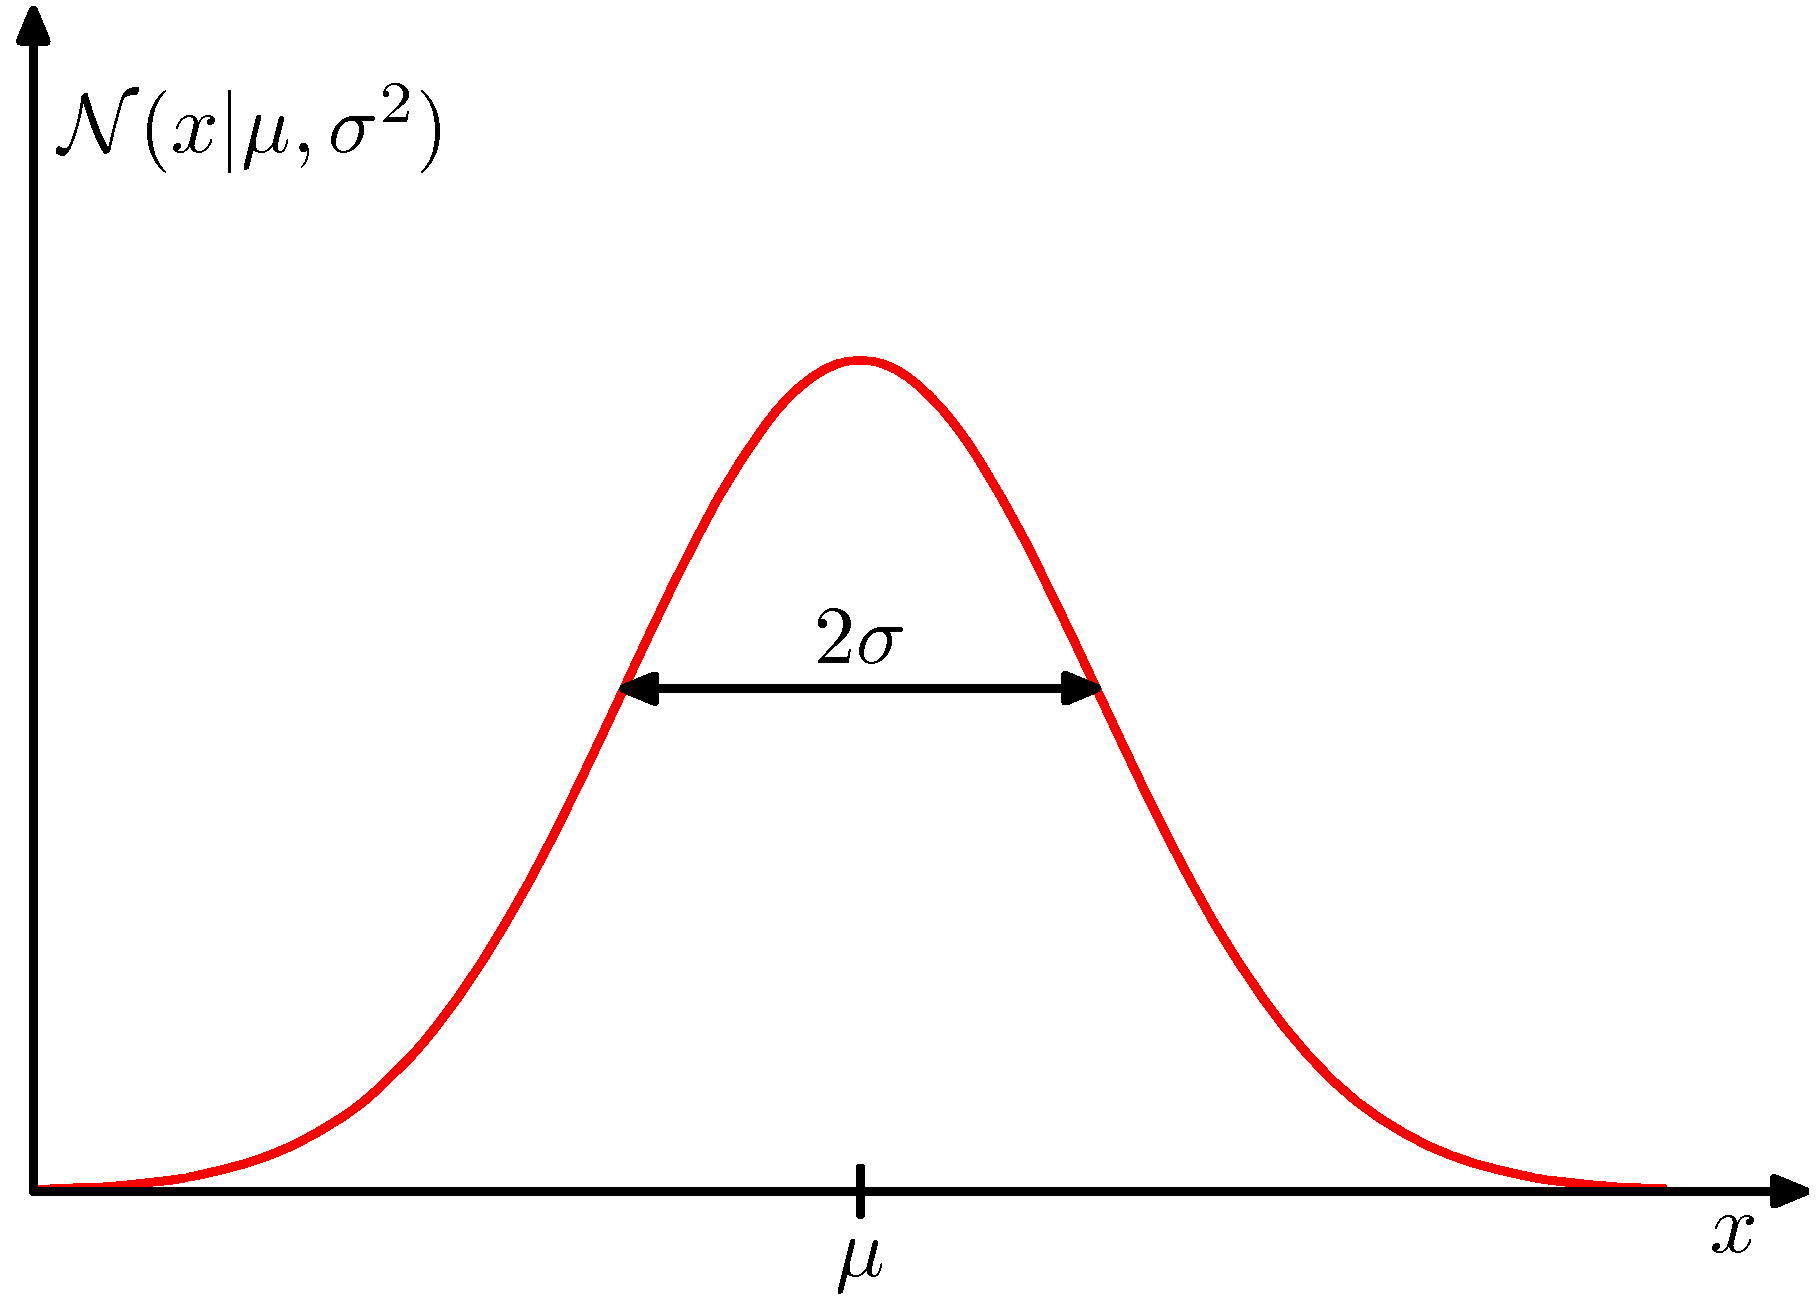
\includegraphics[scale=0.8]{Images/1-13.png}
		\captionsetup{font={small}}
		\caption{标出了均值$\mu$和标准差$\sigma$的高斯分布} 
		\label{fig:1-13}	
	\end{figure}
	\\
	\indent 从(1.46)的形式中我们可以看出,高斯分布满足
	\begin{equation}
		\mathcal{N}(x|\mu,\sigma^2)>0
	\end{equation}
	\indent 而且直接表明了高斯分布是归一化的。所以
	\begin{equation}
		\int_{-\infty}^{\infty}\mathcal{N}(x|\mu,\sigma^2)\ \mathrm{d}x = 1
	\end{equation}
	\indent 所以(1.46)满足概率密度的两项基本要求。\color{red} \textbf{——习题1.7} \color{black}\\
	\indent 我们很快就可以求出服从高斯分布的变量$x$的函数的期望。特别地,$x$的平均值为 \color{red} \textbf{\ \ ——习题1.8} \color{black}
	\begin{equation}
		\mathbb{E}[x]=\int_{-\infty}^{\infty}\mathcal{N}(x|\mu,\sigma^2)x\ \mathrm{d}x = \mu
	\end{equation}
	\indent 由于参数$\mu$表示$x$在该分布下的平均值,实际上就是期望。类似地,其二阶矩
	\begin{equation}
		\mathbb{E}[x^2]=\int_{-\infty}^{\infty}\mathcal{N}(x|\mu,\sigma^2)x^2\ \mathrm{d}x = \mu^2+\sigma^2
	\end{equation}
	\indent 根据(1.49)和(1.50),可以得到$x$的方差为
	\begin{equation}
		\mathrm{var}[x]=\mathbb{E}[x^2]-\mathbb{E}[x]^2=\sigma^2
	\end{equation}
	\indent 于是$\sigma^2$就是方差了。一个分布的最大值被称为模。对于高斯分布而言,其模是在均值处的函数值。\color{red} \textbf{——习题1.9} \color{black}\\
	\indent 我们还希望知道$D$维向量$\mathbf{x}$的高斯分布是怎样定义的。其定义如下:
	\begin{equation}
		\mathcal{N}(\mathbf{x}|\boldsymbol{\mu}, \boldsymbol{\Sigma})=\frac{1}{(2\pi)^{D/2}}\frac{1}{|\boldsymbol{\Sigma}|^{1/2}}\exp\left\{-\frac{1}{2}(\mathbf{x}-\boldsymbol{\mu})^\mathrm{T}\boldsymbol{\Sigma}^{-1}(\mathbf{x}-\boldsymbol{\mu})\right\}
	\end{equation}
	\indent 其中的$D$维向量$\boldsymbol{\mu}$为均值,$D \times D$维矩阵$\boldsymbol{\Sigma}$为协方差,$|\boldsymbol{\Sigma}|$表示$\boldsymbol{\Sigma}$的行列式。我们将在本章节中稍微应用一些多元高斯分布,详细的内容将在第2.3节中学习。\\
	\indent 现在假设我们有一个观测数据集$\boldsymbol{\mathsf{x}}=(x_1,...,x_N)^\mathrm{T}$,表示$N$个对于标量变量$x$的观测。注意,这里我们使用了$\boldsymbol{\mathsf{x}}$这样的符号与$\mathbf{x}$区分开,后者表示对于向量变量$(x_1,...,x_D)^\mathrm{T}$的单一观测。我们假设数据集中所有的观测都是从一个$\mu$和$\sigma^2$都未知的高斯分布中相互独立地抽取出来的,并希望根据这个数据集确定这两个参数。一组从相同的分布中相互独立取出的数据点是独立同分布(independent and identically distributed)的,简称“i.i.d.”。我们已经知道两个独立事件的联合概率是由事件各自的边缘概率求取乘积得到的。由于数据集$\boldsymbol{\mathsf{x}}$是独立同分布的,所以我们可以写出给定$\mu$和$\sigma^2$的条件下该观测出现的概率:
	\begin{equation}
		p(\boldsymbol{\mathsf{x}}|\mu,\sigma^2) = \prod_{n=1}^{N}\mathcal{N}(x_n|\mu,\sigma^2)
	\end{equation}
	\indent 将其视为$\mu$和$\sigma^2$的函数,它就变成了一个高斯分布的似然函数,如图1.14所示。
	\begin{figure}[ht]
		\centering
		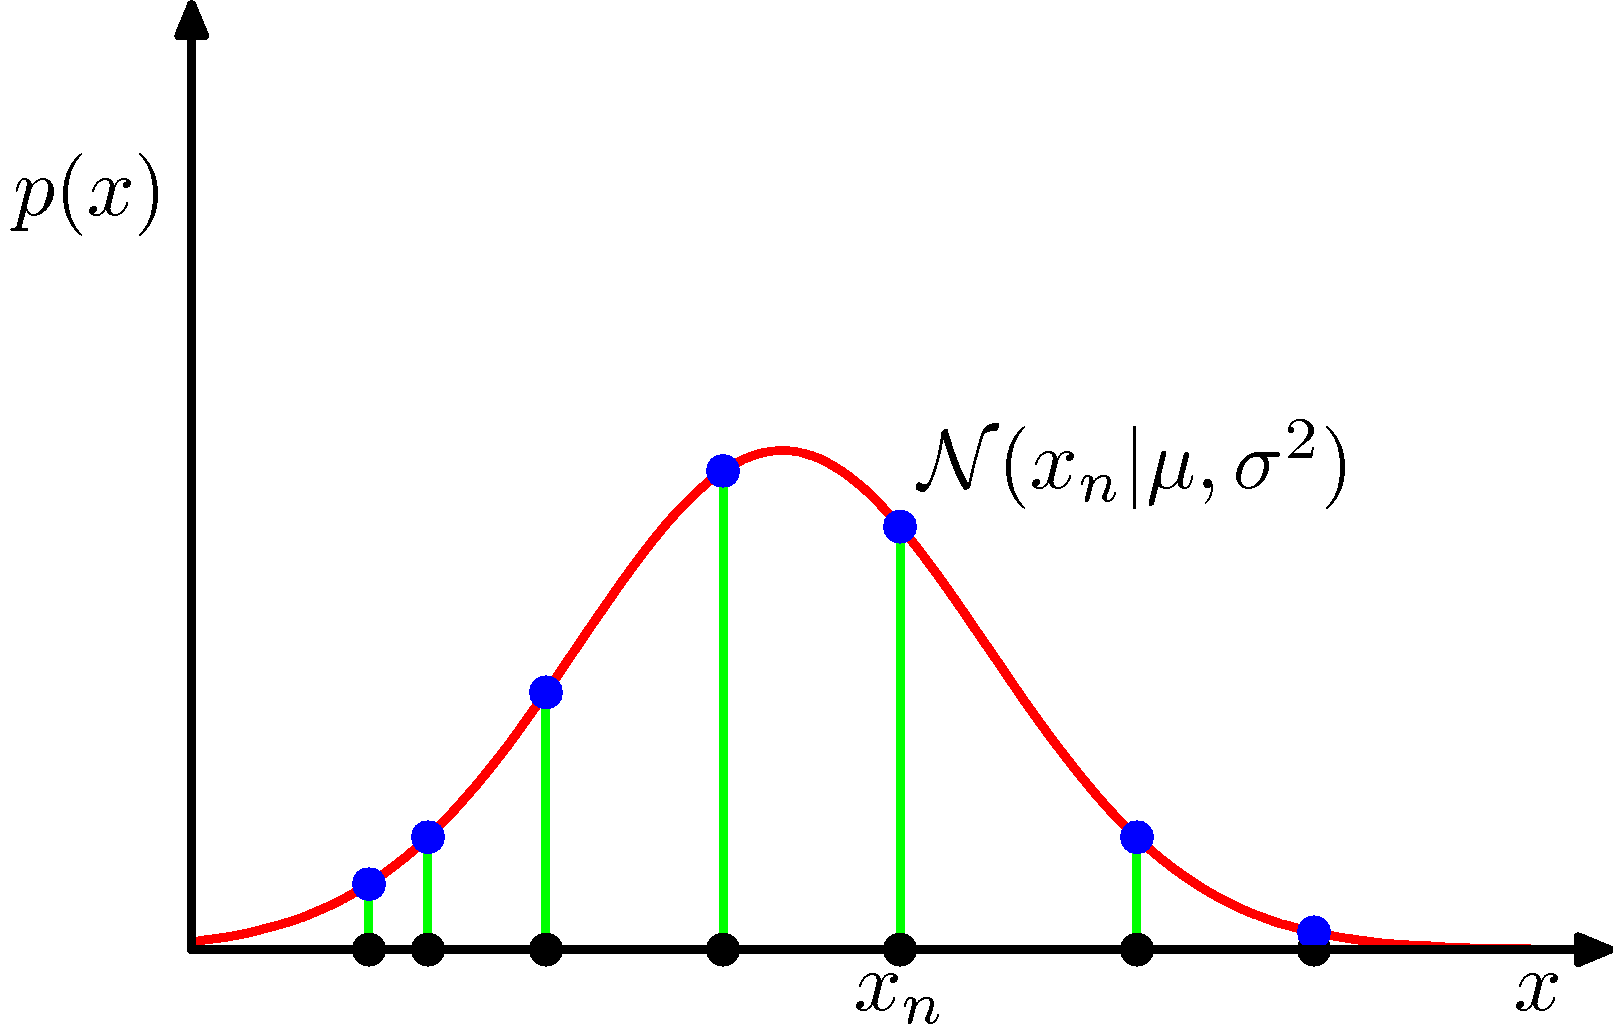
\includegraphics[scale=0.8]{Images/1-14.png}
		\captionsetup{font={small}}
		\caption{高斯分布的似然函数,即图中的红色曲线。黑点表示数据集中的值$\left\{x_n\right\}$,(1.53)中给出的似然函数对应的是图中蓝点的乘积。似然函数最大化的过程也包含了均值和方差的调整,从而使该乘积达到最大值。}
		\label{fig:1-14}	
	\end{figure}
	\\
	\indent 利用观测结果集合进行概率分布中参数的确定,一个常见的办法是找出使得似然函数达到最大值的参数值。这看起来似乎挺奇怪,因为从前面所学的概率论来看,根据给定的数据去求参数的概率最大值似乎更加自然一些,而非根据给定的参数去求数据的概率最大值。事实上,这两个标准是相关的,我们将在后文中结合曲线拟合的例子来讨论这个问题。\color{red} \textbf{——第1.2.5节} \color{black}\\
	\indent 不过,现在我们还是利用(1.53)中似然函数的最大化来确定高斯分布的未知参数$\mu$和$\sigma^2$。在实际应用中,对似然函数的对数求最大值要更方便一些。因为对数函数是单调递增函数,对数函数的最大化与函数自身求取最大化是等价的。求对数不仅简化了随后的分析,而且还利于数值计算,因为大量较小概率的乘积会使计算机的数值精度下降,而对概率对数求和就不会有这样的问题。根据(1.46)和(1.53),对数似然函数可以写成:
	\begin{equation}
		\ln p(\boldsymbol{\mathsf{x}}|\mu,\sigma^2)=-\frac{1}{2\sigma^2}\sum_{n=1}^{N}(x_n-\mu)^2-\frac{N}{2}\ln \sigma^2-\frac{N}{2}\ln(2\pi)
	\end{equation}
	\indent 求(1.54)关于$\mu$的最大值,可以得到最大似然解\color{red} \textbf{\ \ ——习题1.11} \color{black}
	\begin{equation}
		\mu_{\mathrm{ML}}=\frac{1}{N}\sum_{n=1}^{N}x_n
	\end{equation}
	\indent 也就是样本均值(sample mean),即观测值$\left\{x_n\right\}$的均值。类似地,求(1.54)关于$\sigma^2$的最大值,可以得到:
	\begin{equation}
		\sigma_{\mathrm{ML}}^2=\frac{1}{N}\sum_{n=1}^{N}(x_n-\mu_{\mathrm{ML}})^2
	\end{equation}
	\indent 也就是基于样本均值$\mu_{\mathrm{ML}}$的样本方差(sample variance)。需要注意的是,我们要对(1.54)关于$\mu$和$\sigma^2$进行最大化,但对于高斯分布而言,$\mu$的解和$\sigma^2$无关,所以可以先估计(1.55)再利用结果估计(1.56)。\\
	\indent 在本章稍后的内容和以后的章节中,我们将指明最大似然方法有很严重的局限性。现在我们先通过一元高斯分布的最大似然参数解简单阐述一下这个问题。特别地,我们将证明最大似然方法非常整齐划一地低估了分布的方差。这种现象被称为偏移(bias),与多项式曲线拟合问题中的过拟合问题有关。首先注意到,最大似然解$\mu_{\mathrm{ML}}$和$\sigma_{\mathrm{ML}}^2$都是数据集中的值$x_1,...,x_N$的函数。考虑到这两个值基于数据集的期望,而数据集是来自参数为$\mu$和$\sigma^2$的高斯分布的。所以可以直接写出:\color{red} \textbf{——第1.1节, 习题1.12} \color{black}
	\begin{align}
		\mathbb{E}[\mu_{\mathrm{ML}}] &=\mu \\
		\mathbb{E}[\sigma_{\mathrm{ML}}^2]&=\left(\frac{N-1}{N}\right)\sigma^2
	\end{align}
	\indent 于是最大似然估计的均值可以确定正确的期望,但将使估计的方差带有一个系数$(N-1)/N$,所以会比真实值偏低。这个结果背后的原因如图1.15所示。
	\begin{figure}[ht]
		\centering
		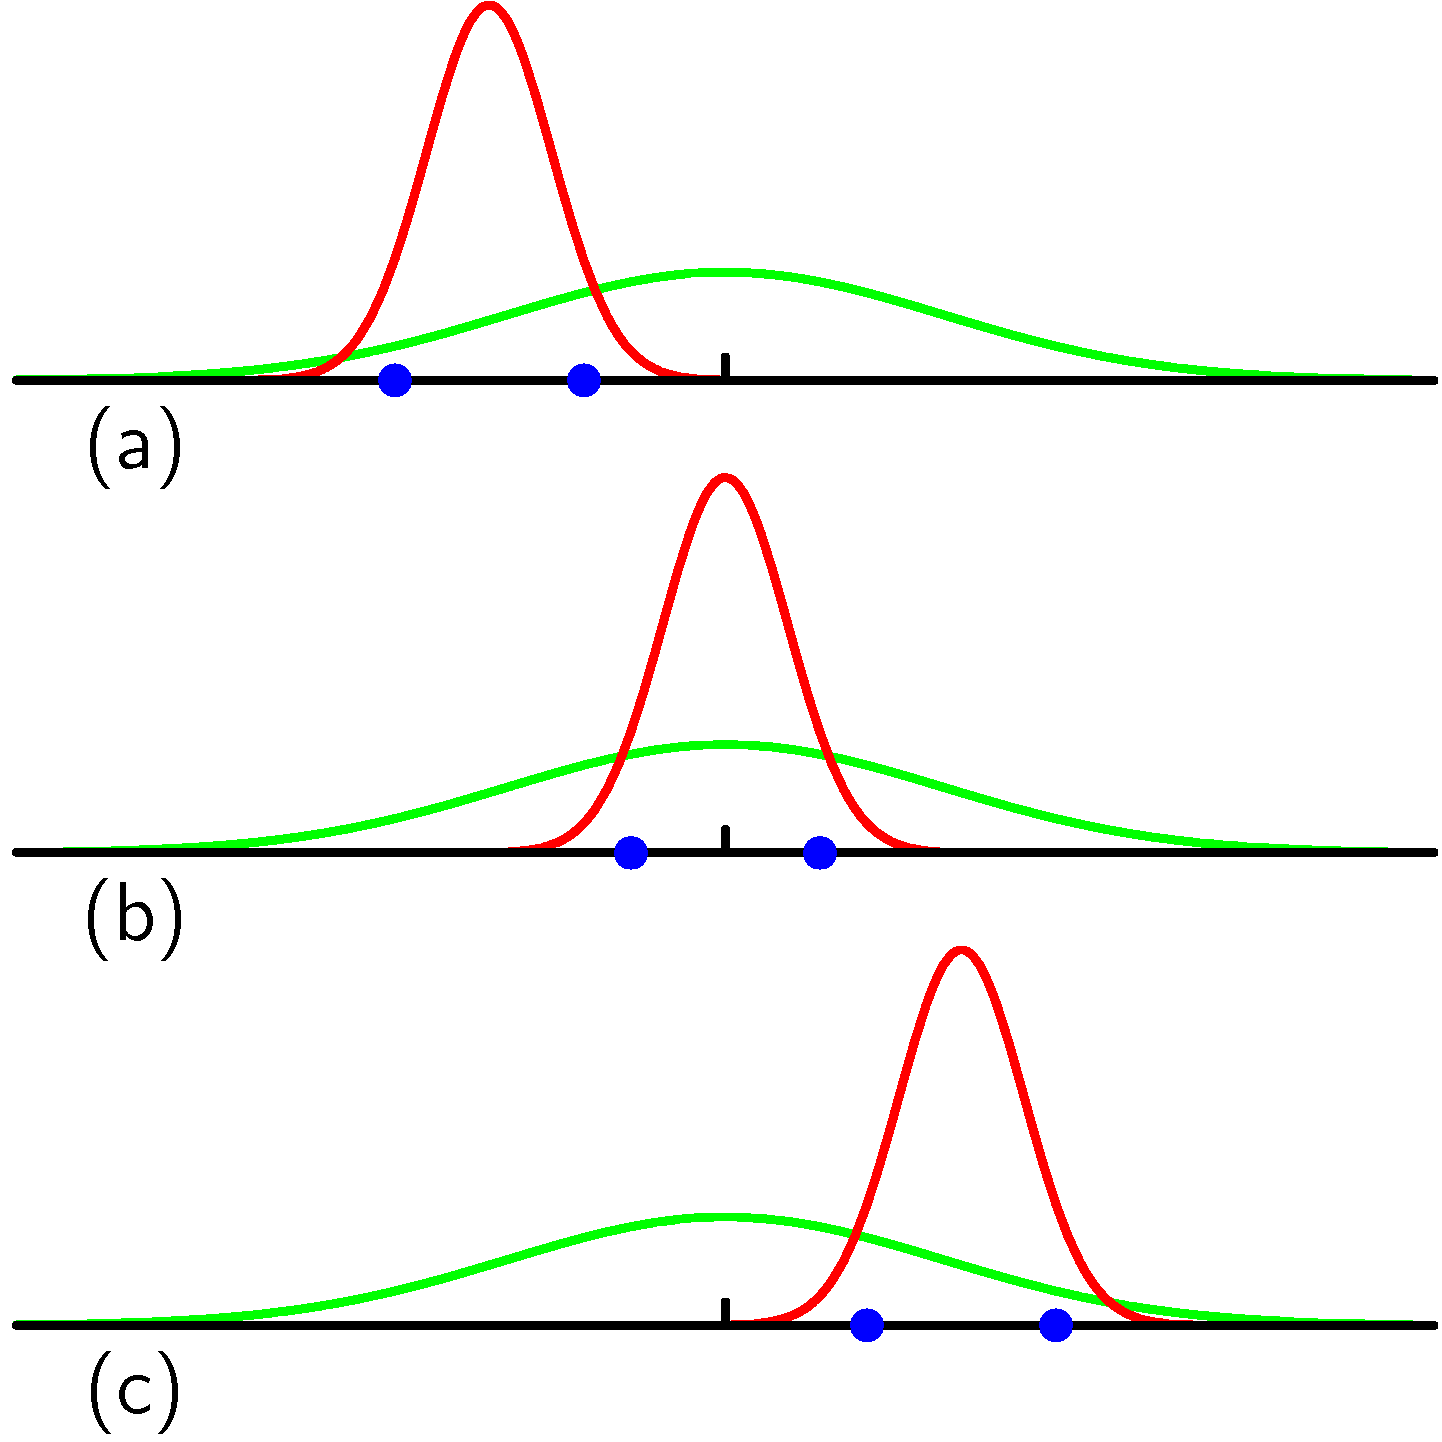
\includegraphics[scale=0.8]{Images/1-15.png}
		\captionsetup{font={small}}
		\caption{在利用最大似然估计确定高斯分布的方差时产生偏移的说明。其中绿色的曲线表示产生数据集的真实高斯分布,三条红色曲线表示基于三个不同的数据集得到的高斯分布拟合结果,每个数据集包含两个数据点,在图中用蓝色的点表示,根据(1.55)和(1.56)给出的结论进行拟合。对三个数据集求平均数,可以看出均值是正确的,但方差被低估了,因为它根据样本均值确定,而非真实的均值。}
		\label{fig:1-15}
	\end{figure}
	\\
	\indent 根据(1.58),下面对于方差参数的估计才是无偏的:
	\begin{equation}
		\widetilde{\sigma}^2 = \frac{N}{N-1}\sigma_{\mathrm{ML}}^2 = \frac{1}{N-1}\sum_{n=1}^{N}(x_n-\mu_{\mathrm{ML}})^2
	\end{equation}
	\indent 在第10.1.3节中我们将看到在应用贝叶斯方法时,这个结果会自然地形成出来。\\
	\indent 需要注意的是,随着数据点数量$N$的增加,最大似然解的偏移将显得越来越不显著,而且当$N \rightarrow \infty$时,方差的最大似然解就是产生数据的分布的方差。在实践中,除非$N$比较小,否则偏移都不会很严重。但是,在本书中,我们对具有很多参数的复杂模型更感兴趣,在这种模型中,最大似然的偏移问题将会比较严重。实际上,我们即将看到,最大似然的偏移问题正是之前讨论的多项式曲线拟合问题中过拟合问题的根源。
	}
	\subsection{重返曲线拟合问题}
	\textnormal{我们已经见证了多项式曲线拟合问题可以用误差最小化的形式表达出来。现在我们返回到曲线拟合的例子中,并通过概率的观点来审视它,从而得到一些关于误差函数和正则化的见解,并将我们引入到完整的贝叶斯方法中。\color{red} \textbf{——第1.1节} \color{black}\\
	\indent 曲线拟合问题的目标,是基于包含有$N$组输入变量$\boldsymbol{\mathsf{x}}=(x_1,...,x_N)^{\mathrm{T}}$及其对应的目标变量$\boldsymbol{\mathsf{t}}=(t_1,...,t_N)^{\mathrm{T}}$的训练数据集,当输入变量$x$有新的取值时,对目标变量$t$进行预测。我们可以利用概率分布,表示目标变量取值的不确定性。对此,我们假设在给定$x$的情况下,对应的$t$服从均值为$y(x,\mathbf{w})$的高斯分布,其中的$y(x,\mathbf{w})$为(1.1)中多项式曲线给出的函数值。于是我们就有:
	\begin{equation}
		p(t|x,\mathbf{w},\beta)=\mathcal{N}(t|y(x,\mathbf{w}),\beta^{-1})
	\end{equation}
	\indent 其中,为了与后面章节中的符号统一,我们定义了一个精确度参数$\beta$,表示该分布的逆方差。图1.16给出了具体的说明。
	\begin{figure}[ht]
		\centering
		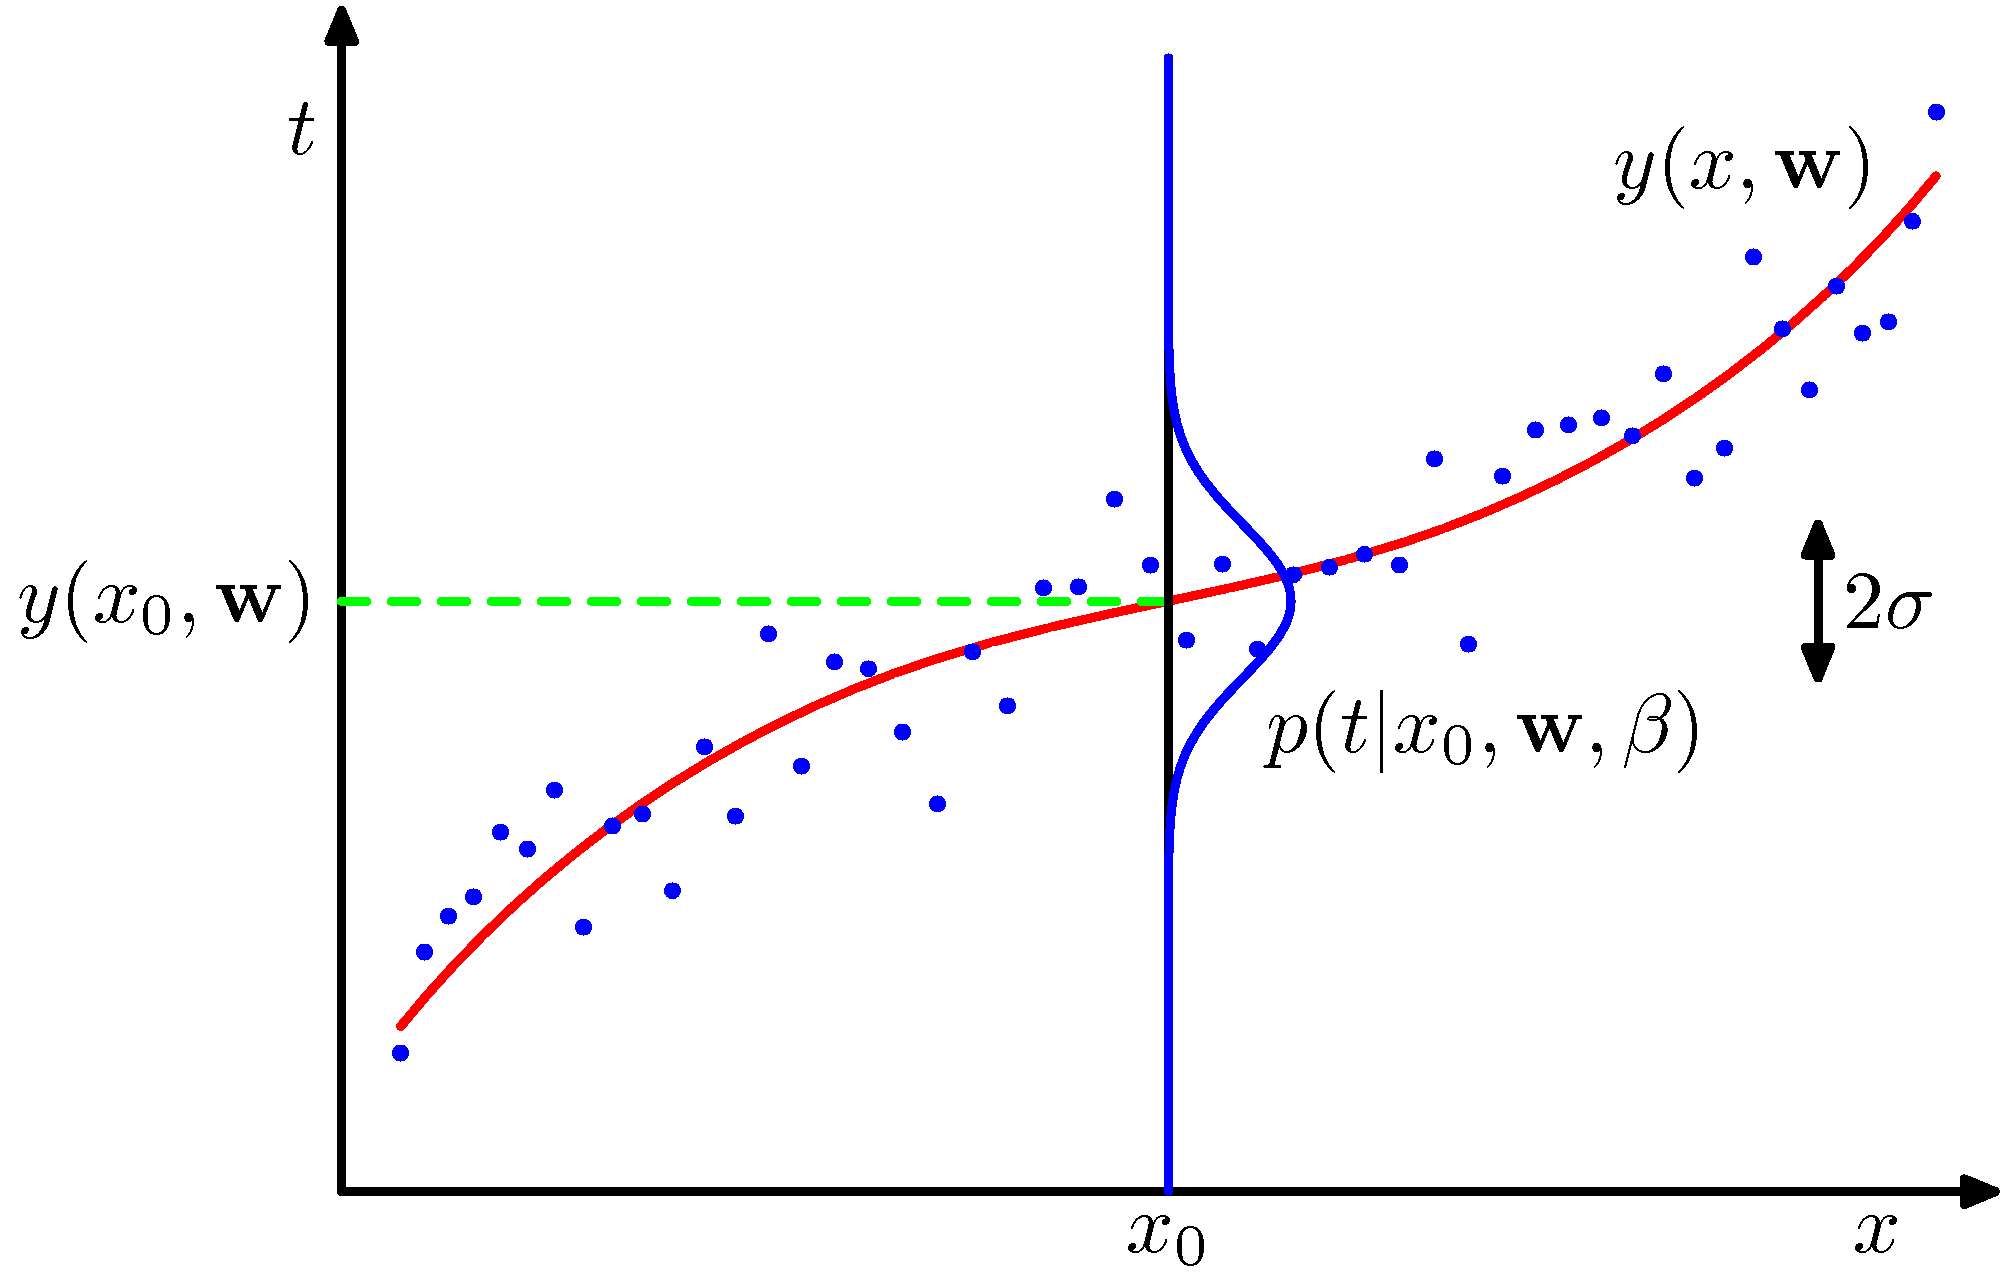
\includegraphics[scale=0.8]{Images/1-16.png}
		\captionsetup{font={small}}
		\caption{(1.60)中给定$x$的情况下$t$的高斯分布。其均值由多项式函数$y(x,\mathbf{w})$给出,$\beta$为与方差相关的精确度参数,$\beta^{-1}=\sigma^2$。}
		\label{fig:1-16}
	\end{figure}
	\\
	\indent 现在基于训练数据$\left\{\boldsymbol{\mathsf{x}},\boldsymbol{\mathsf{t}}\right\}$,利用最大似然来确定未知参数$\mathbf{w}$和$\beta$。如果假设数据是从(1.60)中的分布中相互独立地提取出来的,那么似然函数就可以写成:
	\begin{equation}
		p(\boldsymbol{\mathsf{t}}|\boldsymbol{\mathsf{x}},\mathbf{w},\beta) = \prod_{n=1}^{N}\mathcal{N}(t_n|y(x_n,\mathbf{w}),\beta^{-1})
	\end{equation}
	\indent 正如我们早些时候对于高斯分布的处理一样,对似然函数的对数求最大值要更加方便。根据(1.46)给出的高斯函数的形式,可以写出对数似然函数:
	\begin{equation}
		\ln p(\boldsymbol{\mathsf{t}}|\boldsymbol{\mathsf{x}},\mathbf{w},\beta)=-\frac{\beta}{2}\sum_{n=1}^{N}\left\{y(x_n,\mathbf{w})-t_n\right\}^2 + \frac{N}{2}\ln \beta - \frac{N}{2}\ln(2\pi)
	\end{equation}
	\indent 首先确定多项式系数的最大似然解,用$\mathbf{w}_\mathrm{ML}$来表示。它们是通过对(1.62)关于$\mathbf{w}$进行最大化得到的。所以我们可以省略(1.62)等号右边的后两项,因为这两项与$\mathbf{w}$无关。同时,我们注意到在对数似然函数前面乘一个正数并不影响使得函数取得最大值的$\mathbf{w}$的取值,所以可以用1/2替换系数$\beta/2$。最后,求取对数似然函数的最大值,等价于求取负对数似然函数的最小值。于是对确定的$\mathbf{w}$而言,将似然函数最大化与将(1.2)中定义的平方和误差函数最小化是等价的。因此,平方和误差函数作为在高斯噪声下的最大似然的结果出现了。\\
	\indent 我们同样可以使用最大似然来确定高斯条件分布中的精确度参数$\beta$。关于$\beta$对(1.62)求最大化:
	\begin{equation}
		\frac{1}{\beta_\mathrm{ML}} = \frac{1}{N}\sum_{n=1}^{N}\left\{y(x_n,\mathbf{w}_\mathrm{ML})-t_n\right\}^2
	\end{equation}
	\indent 我们仍然首先确定控制均值的参数向量$\mathbf{w}_\mathrm{ML}$,然后使用它来求取精确度$\beta_\mathrm{ML}$,和此前处理简单高斯分布的情况一样。\color{red} \textbf{——第1.2.4节} \color{black}\\
	\indent 在确定了参数$\mathbf{w}$和$\beta$之后,就可以对新的$x$值做预测了。由于我们有了一个概率模型,所以预测不是以单一点估计的形式,而是由$t$的预测分布(predictive distribution)的形式给出的,而且这个分布是通过将最大似然参数代入(1.60)中得到的:
	\begin{equation}
		p(t|x,\mathbf{w}_\mathrm{ML},\beta_\mathrm{ML})=\mathcal{N}(t|y(x,\mathbf{w}_\mathrm{ML}),\beta_\mathrm{ML}^{-1})
	\end{equation}
	\indent 现在我们向贝叶斯方法更进一步,引入多项式系数$\mathbf{w}$的先验分布。简单起见,考虑如下形式的高斯分布:
	\begin{equation}
		p(\mathbf{w}|\alpha)=\mathcal{N}(\mathbf{w}|\mathbf{0},\alpha^{-1}\mathbf{I})=\left(\frac{\alpha}{2\pi}\right)^{(M+1)/2}\exp\left\{-\frac{\alpha}{2}\mathbf{w}^\mathrm{T}\mathbf{w}\right\}
	\end{equation}
	\indent 其中的$\alpha$是分布的精确度,$M+1$是$M$阶多项式对应的向量$\mathbf{w}$中元素的总数。类似$\alpha$这样的控制分布模型参数的变量称为超参数(hyperparameters)。利用贝叶斯定理,$\mathbf{w}$的后验分布与先验分布和似然函数的乘积成正比:
	\begin{equation}
		p(\mathbf{w}|\boldsymbol{\mathsf{x}},\boldsymbol{\mathsf{t}},\alpha,\beta) \propto p(\boldsymbol{\mathsf{t}}|\boldsymbol{\mathsf{x}},\mathbf{w},\beta)p(\mathbf{w}|\alpha)
	\end{equation}
	\indent 现在可以基于给定数据求取最可能的$\mathbf{w}$值,换句话说,也就是通过后验分布最大化来确定$\mathbf{w}$了。这个方法称为最大后验估计(maximum posterior),简称MAP方法。对(1.66)取负对数,并结合(1.62)和(1.65),我们发现后验的最大值是由以下公式的最小值给出的:
	\begin{equation}
		\frac{\beta}{2}\sum_{n=1}^{N}\left\{y(x_n,\mathbf{w})-t_n\right\}^2 + \frac{\alpha}{2}\mathbf{w}^\mathrm{T}\mathbf{w}
	\end{equation}
	\indent 于是,我们发现后验分布最大化等价于(1.4)中的正则化平方和误差函数最小化,其正则化参数由$\lambda = \alpha/\beta$来确定。
	}
	\subsection{曲线拟合的贝叶斯方法}
	\textnormal{尽管我们已经将先验分布$p(\mathbf{w}|\alpha)$包含了进来,但对于$\mathbf{w}$的估计仍然是点估计,不算是一个贝叶斯方法。在一个完整的贝叶斯方法中,我们应该连贯地应用概率的加法和乘法规则,正如我们即将要看到的一样,这需要我们对所有的$\mathbf{w}$积分。这样的边缘化是模式识别贝叶斯方法的核心。\\
	\indent 在曲线拟合问题中,我们有训练数据$\boldsymbol{\mathsf{x}}$和$\boldsymbol{\mathsf{t}}$和一个新的测试点$x$,我们的目标是预测$t$的值。所以我们希望估计一个预测分布$p(t|x,\boldsymbol{\mathsf{x}},\boldsymbol{\mathsf{t}})$。现在假设参数$\alpha$和$\beta$是固定且已知的(在后续的章节中我们将讨论如何从贝叶斯设定中推断这两个参数)。\\
	\indent 简单来说,贝叶斯方法就是从始至终地运用概率的加法规则和乘法规则,这使得预测分布可以写成如下形式:
	\begin{equation}
		p(t|x,\boldsymbol{\mathsf{x}},\boldsymbol{\mathsf{t}})=\int p(t|x,\mathbf{w})p(\mathbf{w}|\boldsymbol{\mathsf{x}},\boldsymbol{\mathsf{t}})\ \mathrm{d}\mathbf{w}
	\end{equation}
	\indent 其中的$p(t|x,\mathbf{w})$是由(1.60)确定的,同时为了简化,省略了对$\alpha$和$\beta$的依赖。$p(\mathbf{w}|\boldsymbol{\mathsf{x}},\boldsymbol{\mathsf{t}})$是参数的后验分布,可以通过将(1.66)等号右边的式子正则化来得到。我们将在第3.3节中看到,对于类似曲线拟合这样的问题,其后验分布是一个高斯分布,而且可以估计出其解析形式。类似地,(1.68)中的积分同样可以解析表达,于是预测分布可以写成如下形式的高斯分布:
	\begin{equation}
		p(t|x,\boldsymbol{\mathsf{x}},\boldsymbol{\mathsf{t}})=\mathcal{N}(t|m(x),s^2(x))
	\end{equation}
	\indent 其中的均值和方差为:
	\begin{align}
		m(x)&=\beta \phi(x)^\mathrm{T}\mathbf{S}\sum_{n=1}^{N}\phi(x_n)t_n \\
		s^2(x) &= \beta^{-1} + \phi(x)^\mathrm{T}\mathbf{S}\phi(x)
	\end{align}
	\indent 其中的矩阵$\mathbf{S}$为:
	\begin{equation}
		\mathbf{S}^{-1}=\alpha\mathbf{I}+\beta\sum_{n=1}^{N}\phi(x_n)\phi(x_n)^\mathrm{T}
	\end{equation}
	\indent 其中的$\mathbf{I}$为单位矩阵,$\phi(x)$为向量,其元素$\phi_i(x)=x^i,i=0,...,M$。\\
	\indent 由(1.69)可见,预测分布的均值和方差都依赖于$x$。(1.71)中的第一项表示的是由于噪声影响,在估计目标变量$t$时形成的不确定度,此时已经可以用(1.64)中最大似然预测分布的$\beta_{\mathrm{ML}}^{-1}$来表示。然而,公式的第二项来自参数$\mathbf{w}$的不确定度,是贝叶斯处理的结果。关于正弦曲线回归问题的说明如图1.17所示。
	\begin{figure}[H]
		\centering
		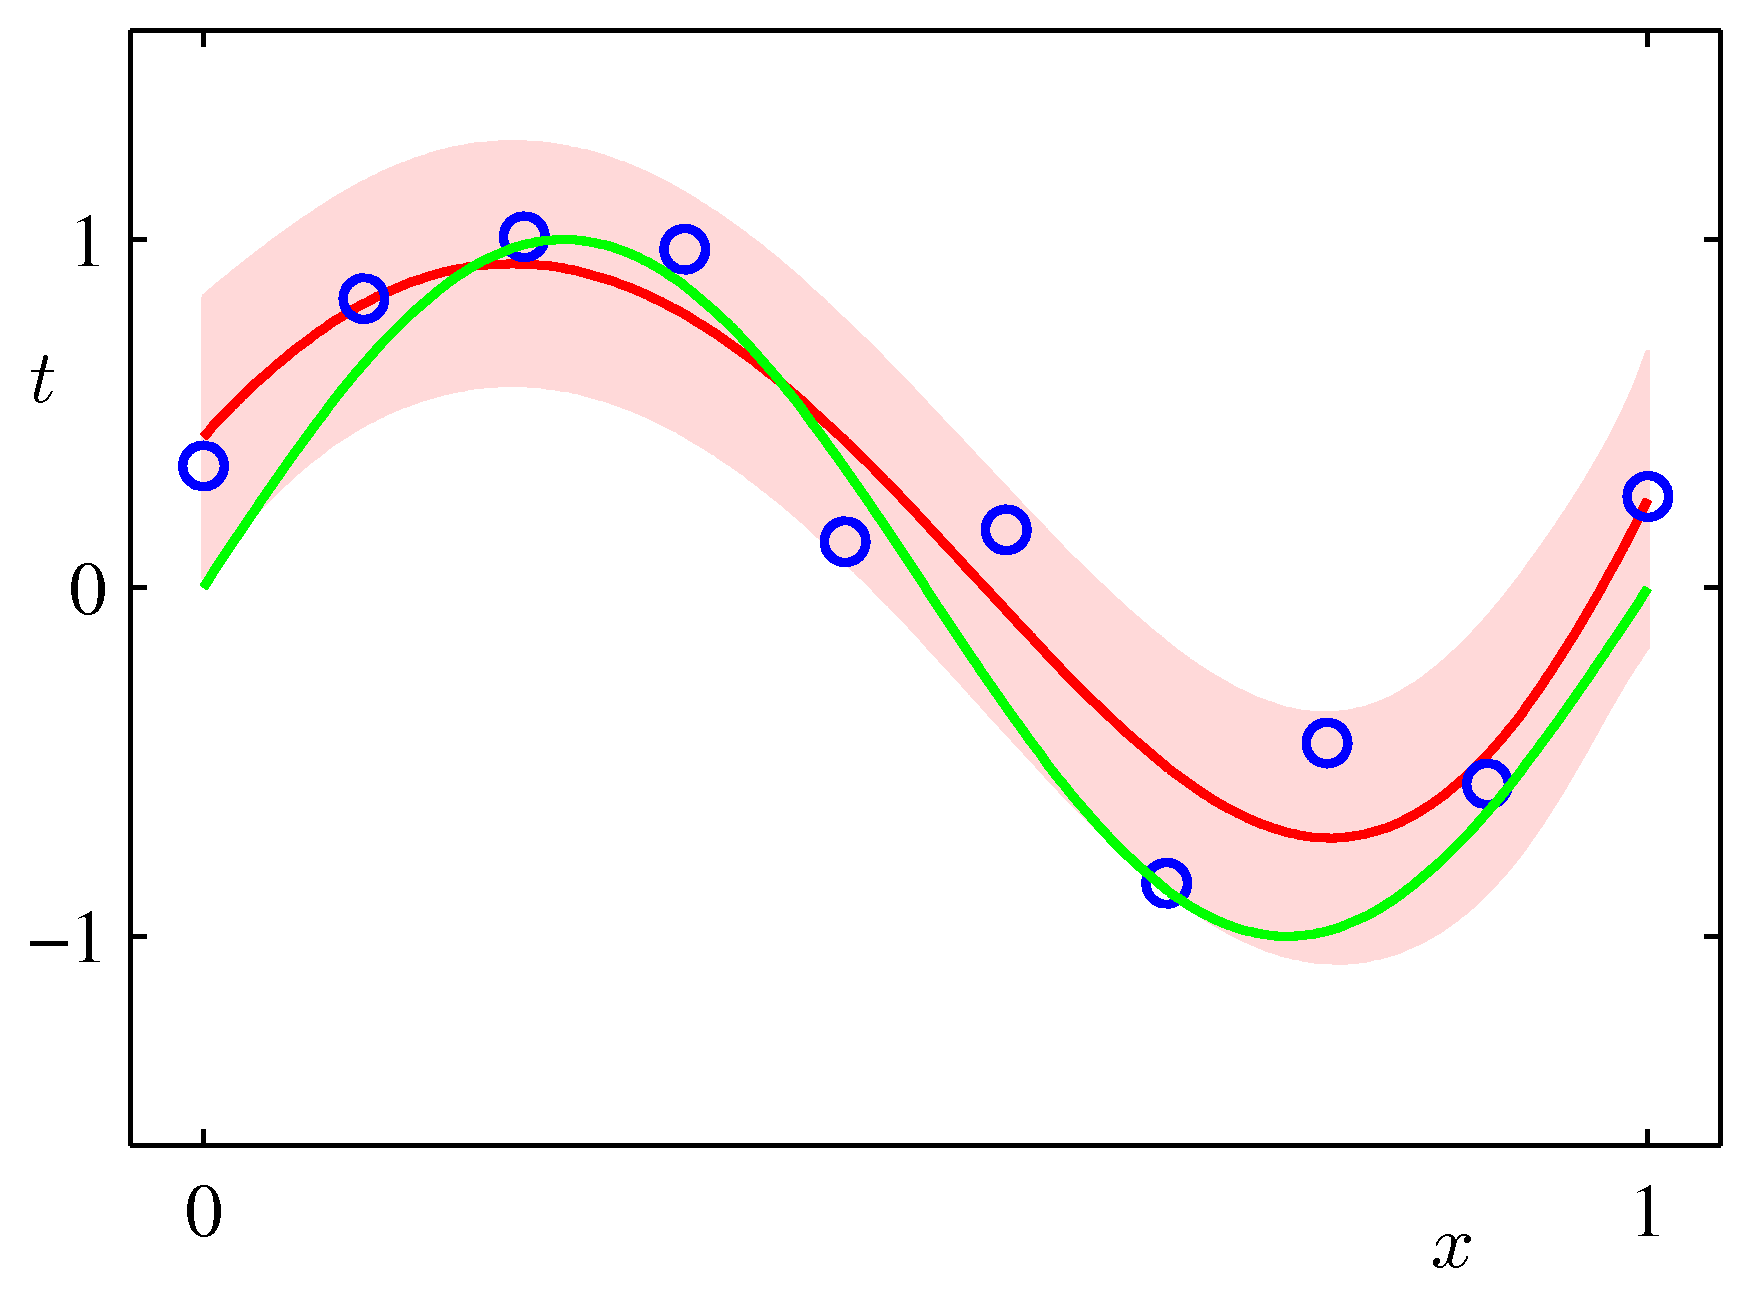
\includegraphics[scale=0.8]{Images/1-17.png}
		\captionsetup{font={small}}
		\caption{利用$M=9$的多项式,利用贝叶斯处理得到的多项式曲线拟合结果,其中,参数$\alpha = 5 \times 10^{-3}$,$\beta = 11.1$(对应于已知的噪声方差),红色的曲线表示预测分布的均值,红色的区域表示平均值附近$\pm1$标准差的区域。}
		\label{fig:1-17}
	\end{figure}
	}
	\section{模型选择}
	\noindent{\color{red} \rule[10pt]{\textwidth}{0.1em}}
	\textnormal{
	\indent 在我们利用最小二乘进行多项式曲线拟合的例子中,可以看到会有一个最优阶数的多项式,使得模型的泛化性能达到最佳。多项式的阶数控制着模型中自由参数的个数,所以也控制着模型的复杂度。在正则化最小二乘中,正则化系数$\lambda$同样也控制着模型的复杂度。而对于更加复杂的模型,例如混合分布和神经网络,更是可能存在更多的控制模型复杂度的参数。在实际应用中,我们需要确定这些参数,从而使得模型对于新的数据具有最优的预测性能。此外,除了对一个给定模型寻求合适的复杂度参数,我们还希望同时考虑一系列不同类型的模型,以便为特定的应用找到最佳的模型。\\
	\indent 我们已经在最大似然方法中看到,由于过拟合问题的存在,模型在训练集上的性能并不能真实反映出其在未知数据上的预测性能。如果数据充足,那么一种方法是使用一些现有的数据训练一系列的模型,或者给出某个复杂度参数下多组参数的模型,然后在独立出来的数据(有时称为验证(validation)集)上进行比较,并选择预测性能最优的那一个。如果使用一个大小有限的数据集在模型设计时进行多次的迭代,就可能出现对验证数据过拟合的现象,所以有必要提前把第三个数据集——测试集(test set)独立取出,最后再用于评估所选模型的性能。\\
	\indent 然而在很多应用中,用于训练和测试的数据会不太够用。在这种情形下,还想要构建好的模型,我们就希望能够用尽可能多的数据去训练。然而,如果验证集太小,那么模型对于预测性能的估计就是附带有噪声的。对这种进退两难的情况,一种解法是利用交叉验证(cross-validation),如图1.18所示。这种方法使得$(S-1)/S$的数据可以用于训练,同时还可以让所有数据都可以用于评估模型性能。当数据特别稀缺时,留一法(leave-one-out)是比较合适的,也就是使$S$等于数据点总数$N$。
	\begin{figure}[ht]
		\centering
		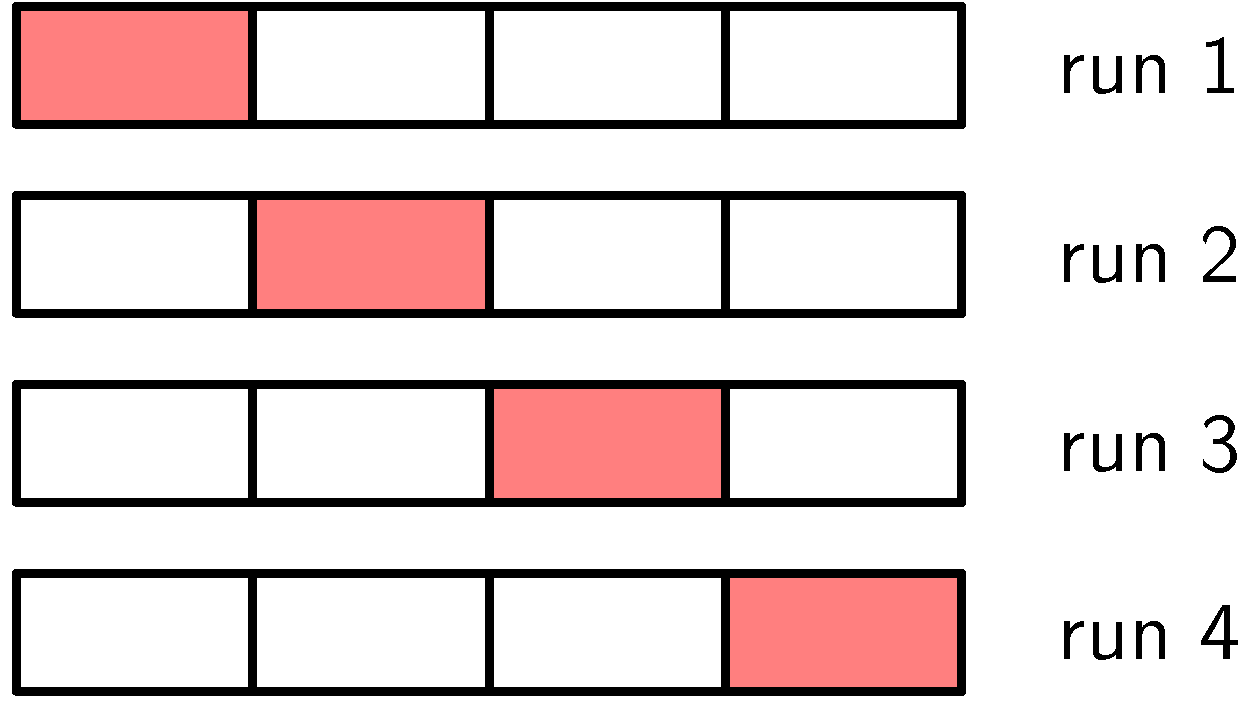
\includegraphics[scale=0.8]{Images/1-18.png}
		\captionsetup{font={small}}
		\caption{以$S=4$为例的$S$重交叉验证,将可用数据划分为$S$组(最简单的办法是平均分配,每组的数据数量一样)。于是$S-1$组的数据可以用于训练模型,剩下的组用于评估。然后对于留出组(红色方块)的所有$S$种可能的情况重复这个过程,最后对$S$次实验中的性能得分取平均数。}
		\label{fig:1-18}
	\end{figure}
	\\
	\indent 交叉验证的一个主要缺点是使训练的次数增加了$S$倍,这对于本身计算量就很大的模型来说就是很有问题的。类似于交叉验证这样将数据拆分来验证性能的做法还有一个问题是,对于一个模型可能会有多个复杂度参数(举例来说,可能会有好几个正则化参数)。在最坏的情况下,寻找这些参数的组合可能会需要参数数量指数倍的训练。很明显,我们需要更好的办法。在理想情况下,这个办法应该仅依赖于训练数据,而且允许在单个的训练中比较多个具有不同超参数和类型的模型。因此我们需要找到一种性能指标,它应该仅依赖于训练数据,而且不会因过拟合而造成偏差。\\
	\indent 历史上已经提出了很多个“信息标准”,试图通过惩罚项来校正最大似然的偏差,以弥补复杂模型的过拟合问题。例如Akaike信息标准,即AIC(Akaike, 1974),会选择如下值取得最大的模型:
	\begin{equation}
		\ln p(\mathcal{D}|\mathbf{w}_{\mathrm{ML}}) -M
	\end{equation}
	\indent 其中的$p(\mathcal{D}|\mathbf{w}_{\mathrm{ML}})$为最优拟合的对数似然,$M$为模型中的可调参数的数量。贝叶斯信息标准(BIC)是这个值的变体,将在第4.4.1节中讨论。然而,这些标准并没有考虑模型参数的不确定性,在实际应用中更加适合简单的模型。我们将在第3.4节中使用完整的贝叶斯方法,那时我们将看到复杂度的惩罚项可以自然且合理地出现。
	}
	\section{维数灾难}
	\noindent{\color{red} \rule[10pt]{\textwidth}{0.1em}}
	\textnormal{
	\indent 在多项式曲线拟合的案例中只有一个输入变量$x$。然而在模式识别的实际应用中,我们通常需要应对包含有很多输入变量的高维空间。现在我们要讨论的就是高维的输入会带来相当严峻的挑战,而且是影响模式识别技术设计的重要因素。\\
	\indent 为了说明这个问题,我们引入一个生成好的数据集,这个数据集中的数据来自一个油、水、气混合物的运输管道(Bishop and James, 1993)。这三种物质都能够以“均质”、“环状物”和“层状物”三种不同的几何构型中的一种存在,而且三种物质的比例也会随之变化。每个数据点都是一个包含了Gamma射线密度计测量结果的12维输入向量,所述的测量结果是Gamma射线密度计测量通过管道的Gamma射线的衰减得到的。这个数据集的详细叙述详见附录A。如图1.19所示为来自该数据集的100个点各自的两项测量结果$x_6$和$x_7$。为了简洁起见,剩下的10项测量结果均被忽略。每个数据点都根据它属于哪一种几何构型进行了标记,我们的目的是使用这些数据作为训练集,从而对新的($x_6,x_7$)进行分类,就像图1.19中的“$\times$”一样。可以观察到那个“$\times$”周围是很多的红色的点,所以我们应该会假设它是属于“红色”类别的。然而,它的周围也有很多绿色的点,所以把它归类为“绿色”也是可以的,不过把它归类为“蓝色”似乎是不太可能了。在这里我们的直觉是,训练集中“$\times$”周围的点对于“$\times$”类别的影响应该更强,反之亦然。其实这个直觉是正确的,我们将在稍后的章节中讨论这个问题。\\
	\indent 那我们应该如何将这种直觉转化为学习算法呢?一个比较简单的办法是将输入空间分割成如图1.20所示的那种规则的元组。当我们拿到一个测试点并进行类别的预测时,首先确定它属于哪一个元组,然后找到这个元组中全部的训练数据。测试点的类别就会被预测为该元组不同类别的训练点中数量最多的那个类别。
	\begin{figure}[ht]
		\centering
		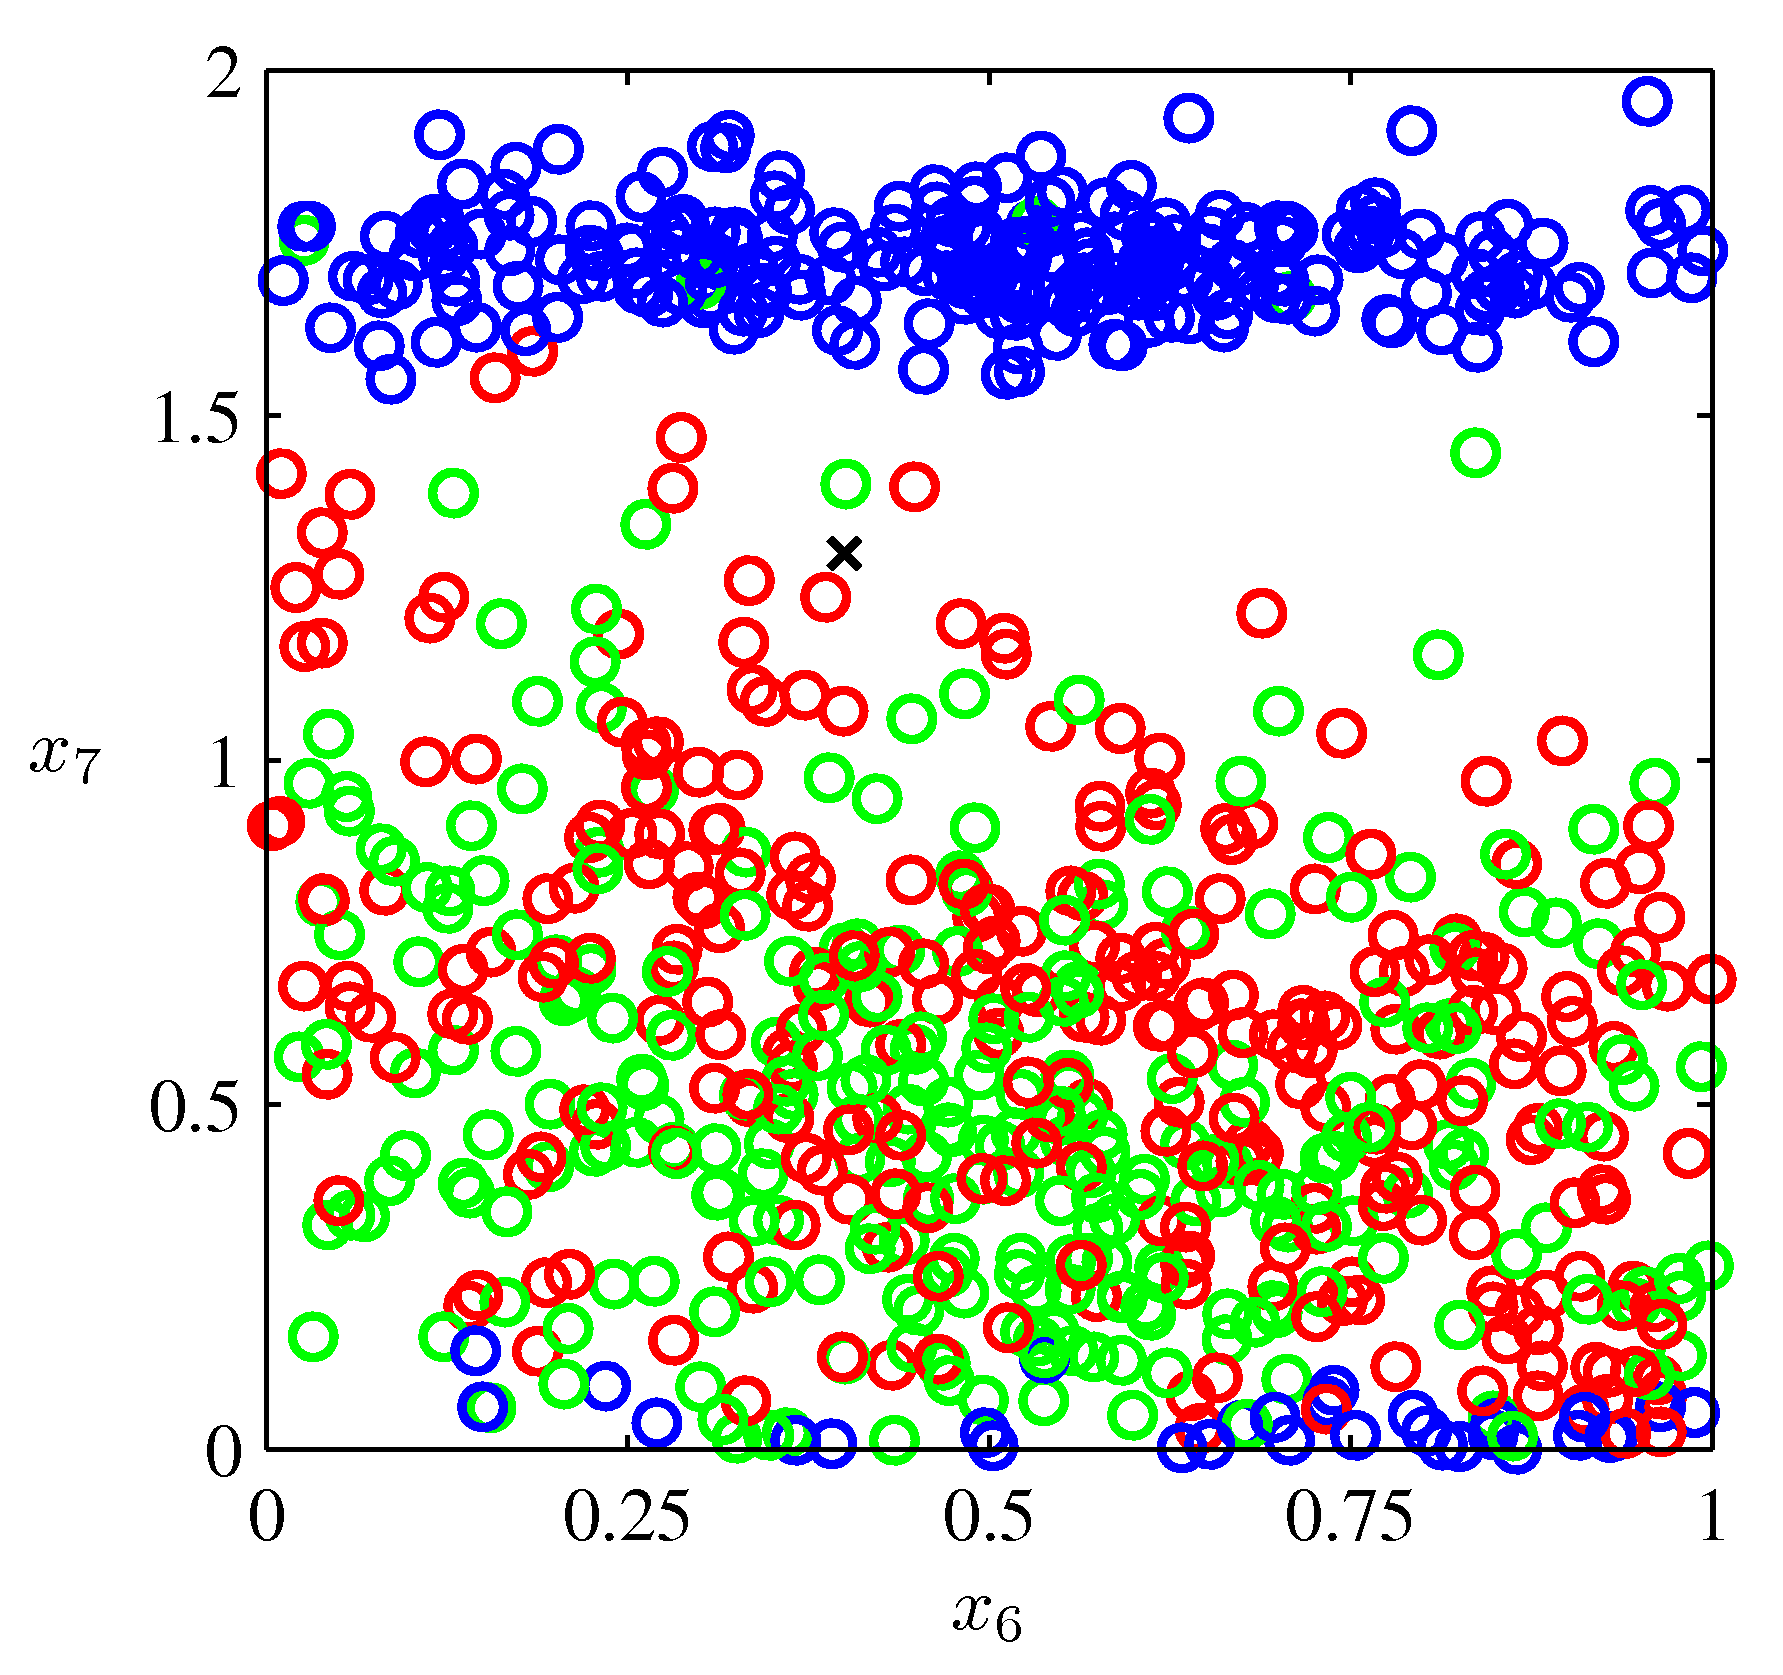
\includegraphics[scale=0.8]{Images/1-19.png}
		\captionsetup{font={small}}
		\caption{来自油流数据的输入量$x_6$,$x_7$的散点图,其中红色表示“均质”类,绿色代表“环状物”类,蓝色代表“层状物”类,我们的目标是将新的数据点“$\times$”进行分类。}
		\label{fig:1-19}
		\centering
		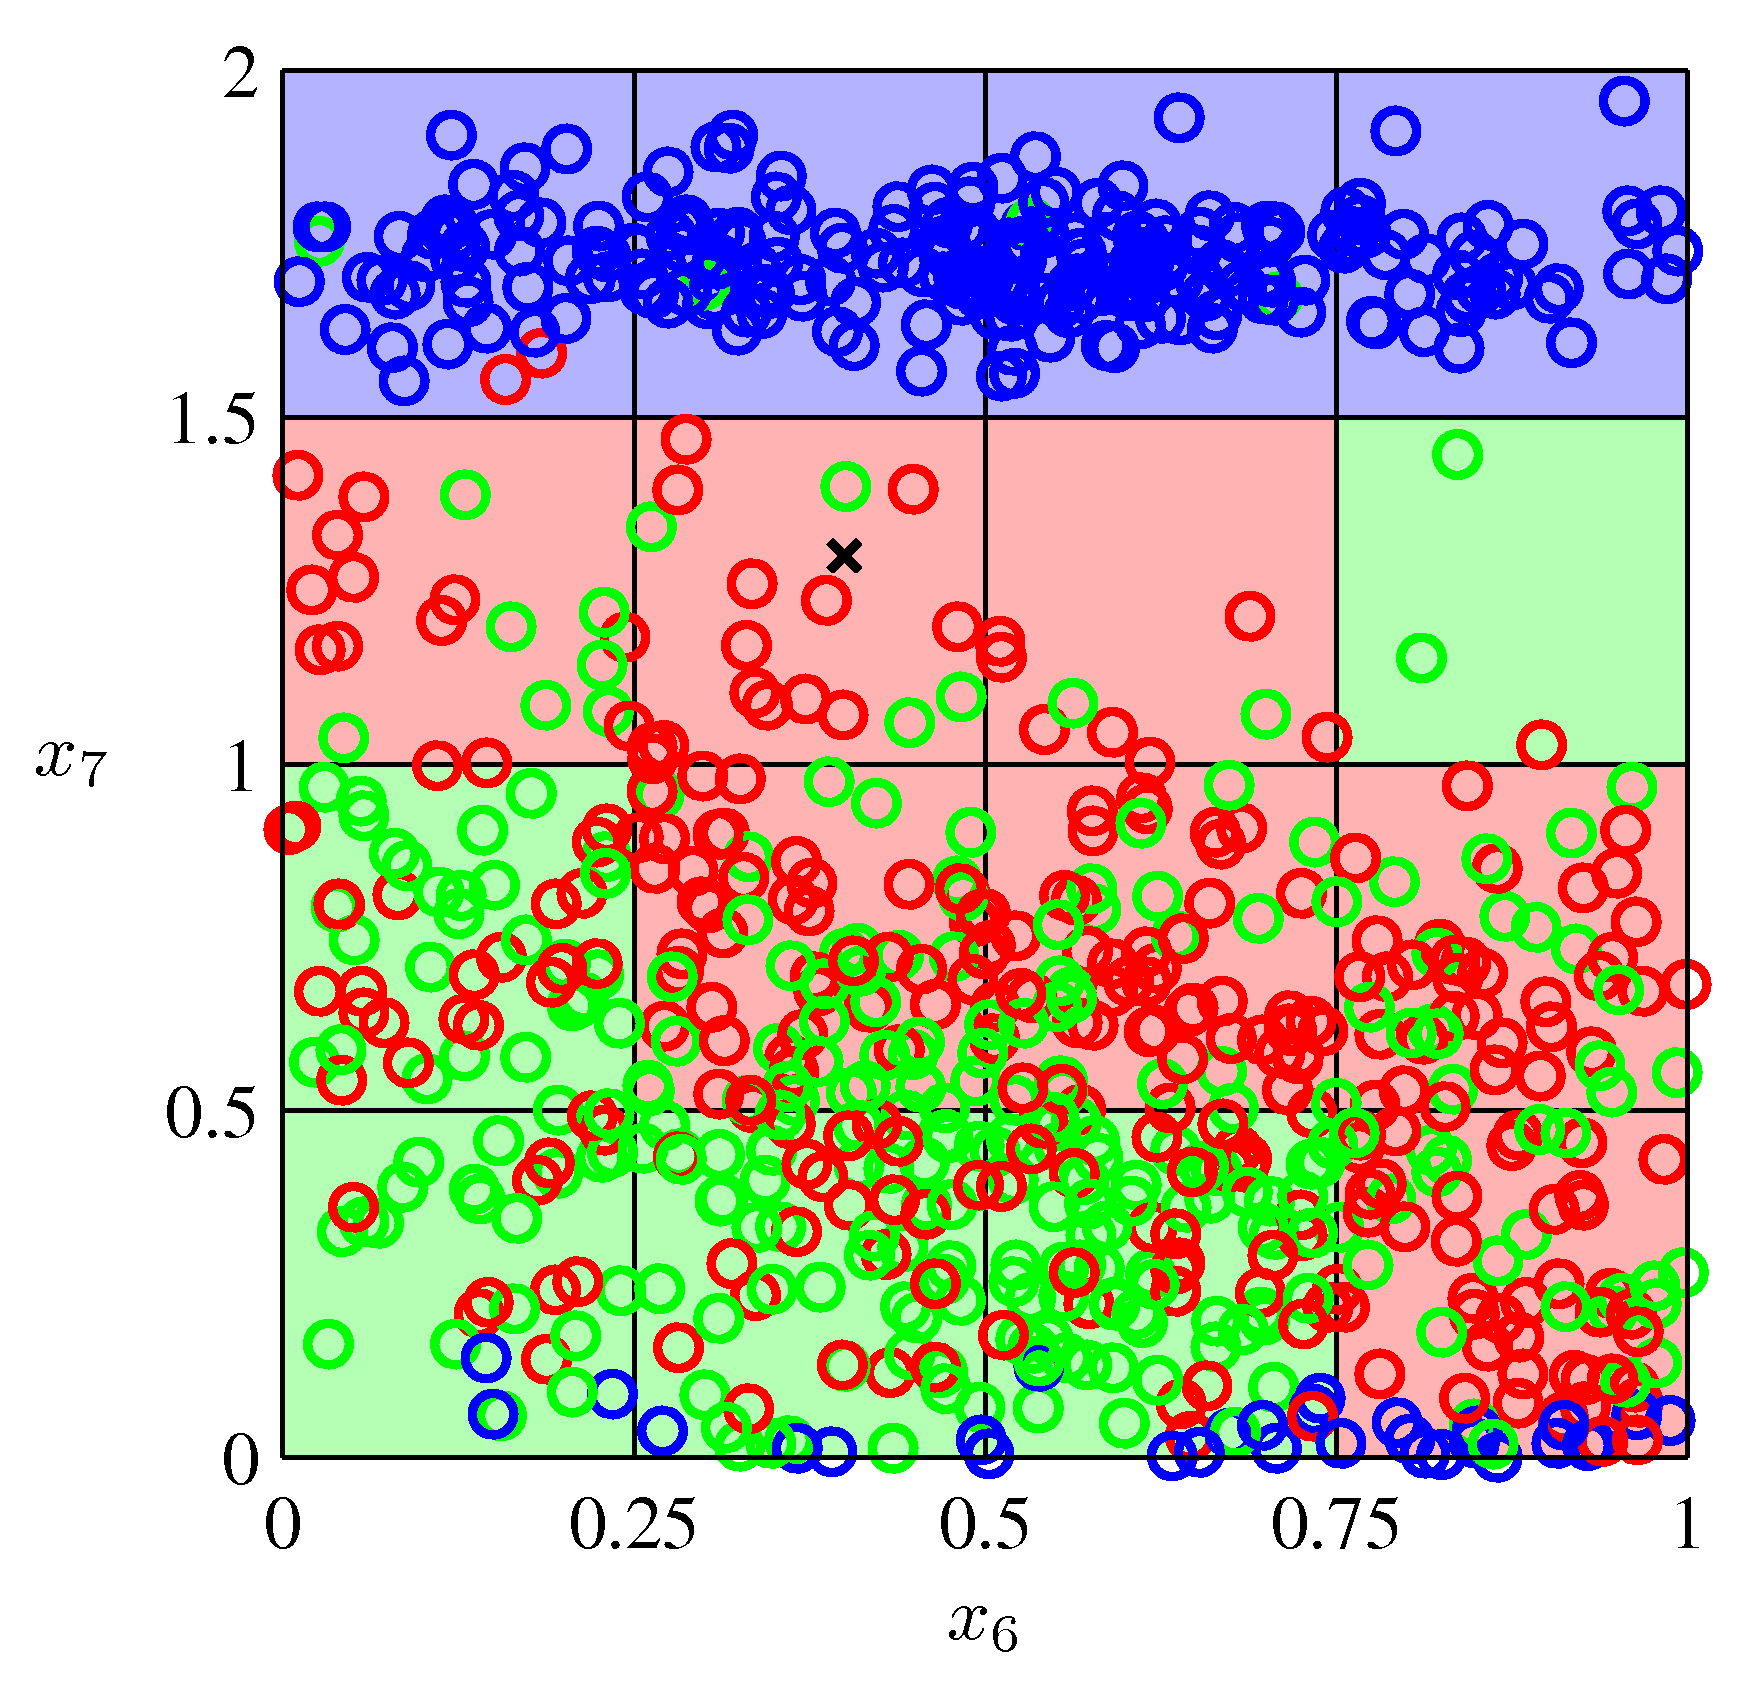
\includegraphics[scale=0.8]{Images/1-20.png}
		\captionsetup{font={small}}
		\caption{对于上述分类问题的一个简单方法,其中输入空间被划分成若干元组,对于任何的新测试点,其类别都会被预测为其所在元组中数量最多的那种数据点的类别。很快我们就会看到这样的办法有很多致命的缺点。}
		\label{fig:1-20}
	\end{figure}
	\\
	\indent 这个朴素的方法有成吨的问题。其中最要命的问题就是,当问题的输入变量数量变大时,对应地会使输入空间的维度变高。如图1.21所示就是这个问题的原始形态。其中展示了如果将空间区域分割成规则的元组,那么元组的数量会随着空间维度的上升而呈指数型地上涨。这样带来的问题是我们需要一个超级大的训练集才能保证元组是非空的。很明显,这样的办法在输入空间维度稍微高一点的时候就完蛋了,需要找到更好的办法。
	\begin{figure}[ht]
	\centering
		\begin{minipage}[t]{0.3\linewidth}
		\centering
		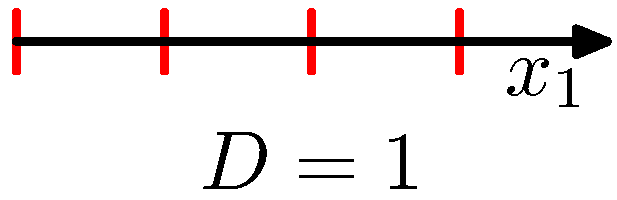
\includegraphics[scale=0.8]{Images/1-21a.png}
		\label{fig:1-21a}
		\end{minipage}
		\begin{minipage}[t]{0.3\linewidth}
		\centering
		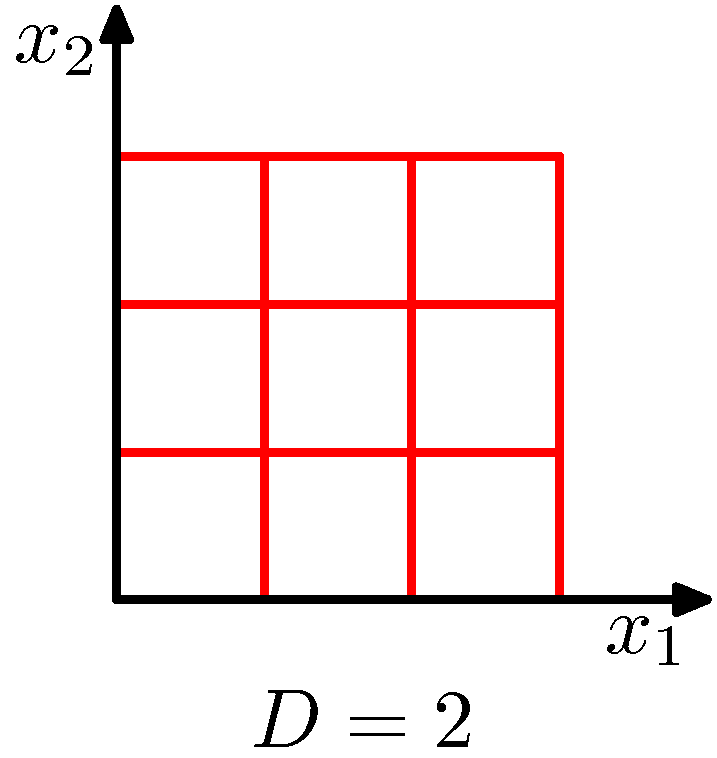
\includegraphics[scale=0.8]{Images/1-21b.png}
		\label{fig:1-21b}
		\end{minipage} 
		\centering
		\begin{minipage}[t]{0.3\linewidth}
		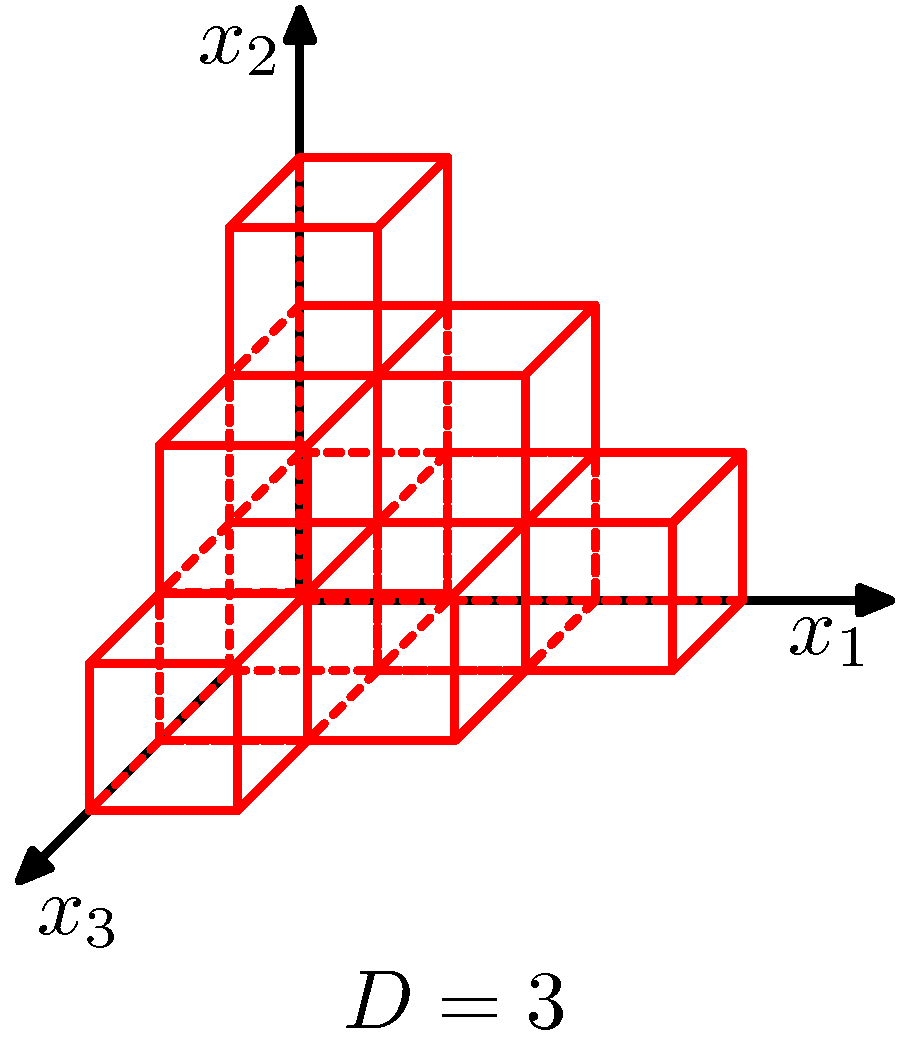
\includegraphics[scale=0.8]{Images/1-21c.png}
		\label{fig:1-21c}
		\end{minipage}
		\captionsetup{font={small}}
		\caption{维数灾难的示意图,展示了区域中格子的数量如何随着空间维度$D$的上升而呈指数型上涨。为了简洁,这里仅展示到$D=3$的情况。}
	\end{figure}
	\\
	\indent 对于高维空间的问题,我们可以通过回看多项式曲线拟合的案例来得到更加深刻的见解,同时研究一下如何将这项方法进行扩展,从而应对具有多个变量的输入空间。\color{red} \textbf{——第1.1节} \color{black}如果有$D$个输入变量,那么三阶多项式的通式为:
	\begin{equation}
		y(\boldsymbol{\mathrm{x}},\boldsymbol{\mathrm{w}})=w_0 + \sum_{i=1}^{D}{w_ix_i} + \sum_{i=1}^{D} \sum_{j=1}^{D}{w_{ij}x_ix_j} + \sum_{i=1}^{D}\sum_{j=1}^{D}\sum_{k=1}^{D}{w_{ijk}x_ix_jx_k}
	\end{equation}
	\indent 当$D$增加时,独立系数的数量(由于$x$变量之间的交换对称性,并非所有系数都是独立的)会按比例增加到$D^3$。在实践中,为了获取数据中复杂的依赖关系,可能会需要使用更高阶的多项式。对于一个阶数为$M$的多项式,系数的数量就会上升为$D^M$这样的了。\color{red} \textbf{——习题 1.16} \color{black}尽管现在是一个幂次上涨而非指数上涨,但躲得了初一躲不了十五,这个办法也会很快变得笨拙,在实用方面受到限制。\\
	\indent 在三维空间的显现实生活中形成的几何直觉会在我们研究高维空间时遭遇严重的打击。一个简单的例子是,对于一个$D$维空间中半径$r=1$的球体,求球体中位于$r=1-\epsilon$与$r=1$之间的体积。我们注意到$D$维空间中半径为$r$的球体体积单位一定是$r^D$,所以可以这样写:
	\begin{equation}
		V_D(r)=K_Dr^D
	\end{equation}
	其中系数$K_D$仅与$D$有关。于是所要求的体积可以写成:\color{red} \textbf{——习题 1.18} \color{black}
	\begin{equation}
		\frac{V_D(1)-V_D(1-\epsilon)}{V_D(1)}=1-(1-\epsilon)^D
	\end{equation}
	它可以被认为是在$D$取得不同数值时的$\epsilon$的函数,如图1.22所示。可以看出,对于较大的$D$,所求体积即使在$\epsilon$很小的情况下都是接近1的。于是,在高维的空间中,一个球体的大部分体积都集中在靠近表面的薄壳中!
	\begin{figure}[ht]
		\centering
		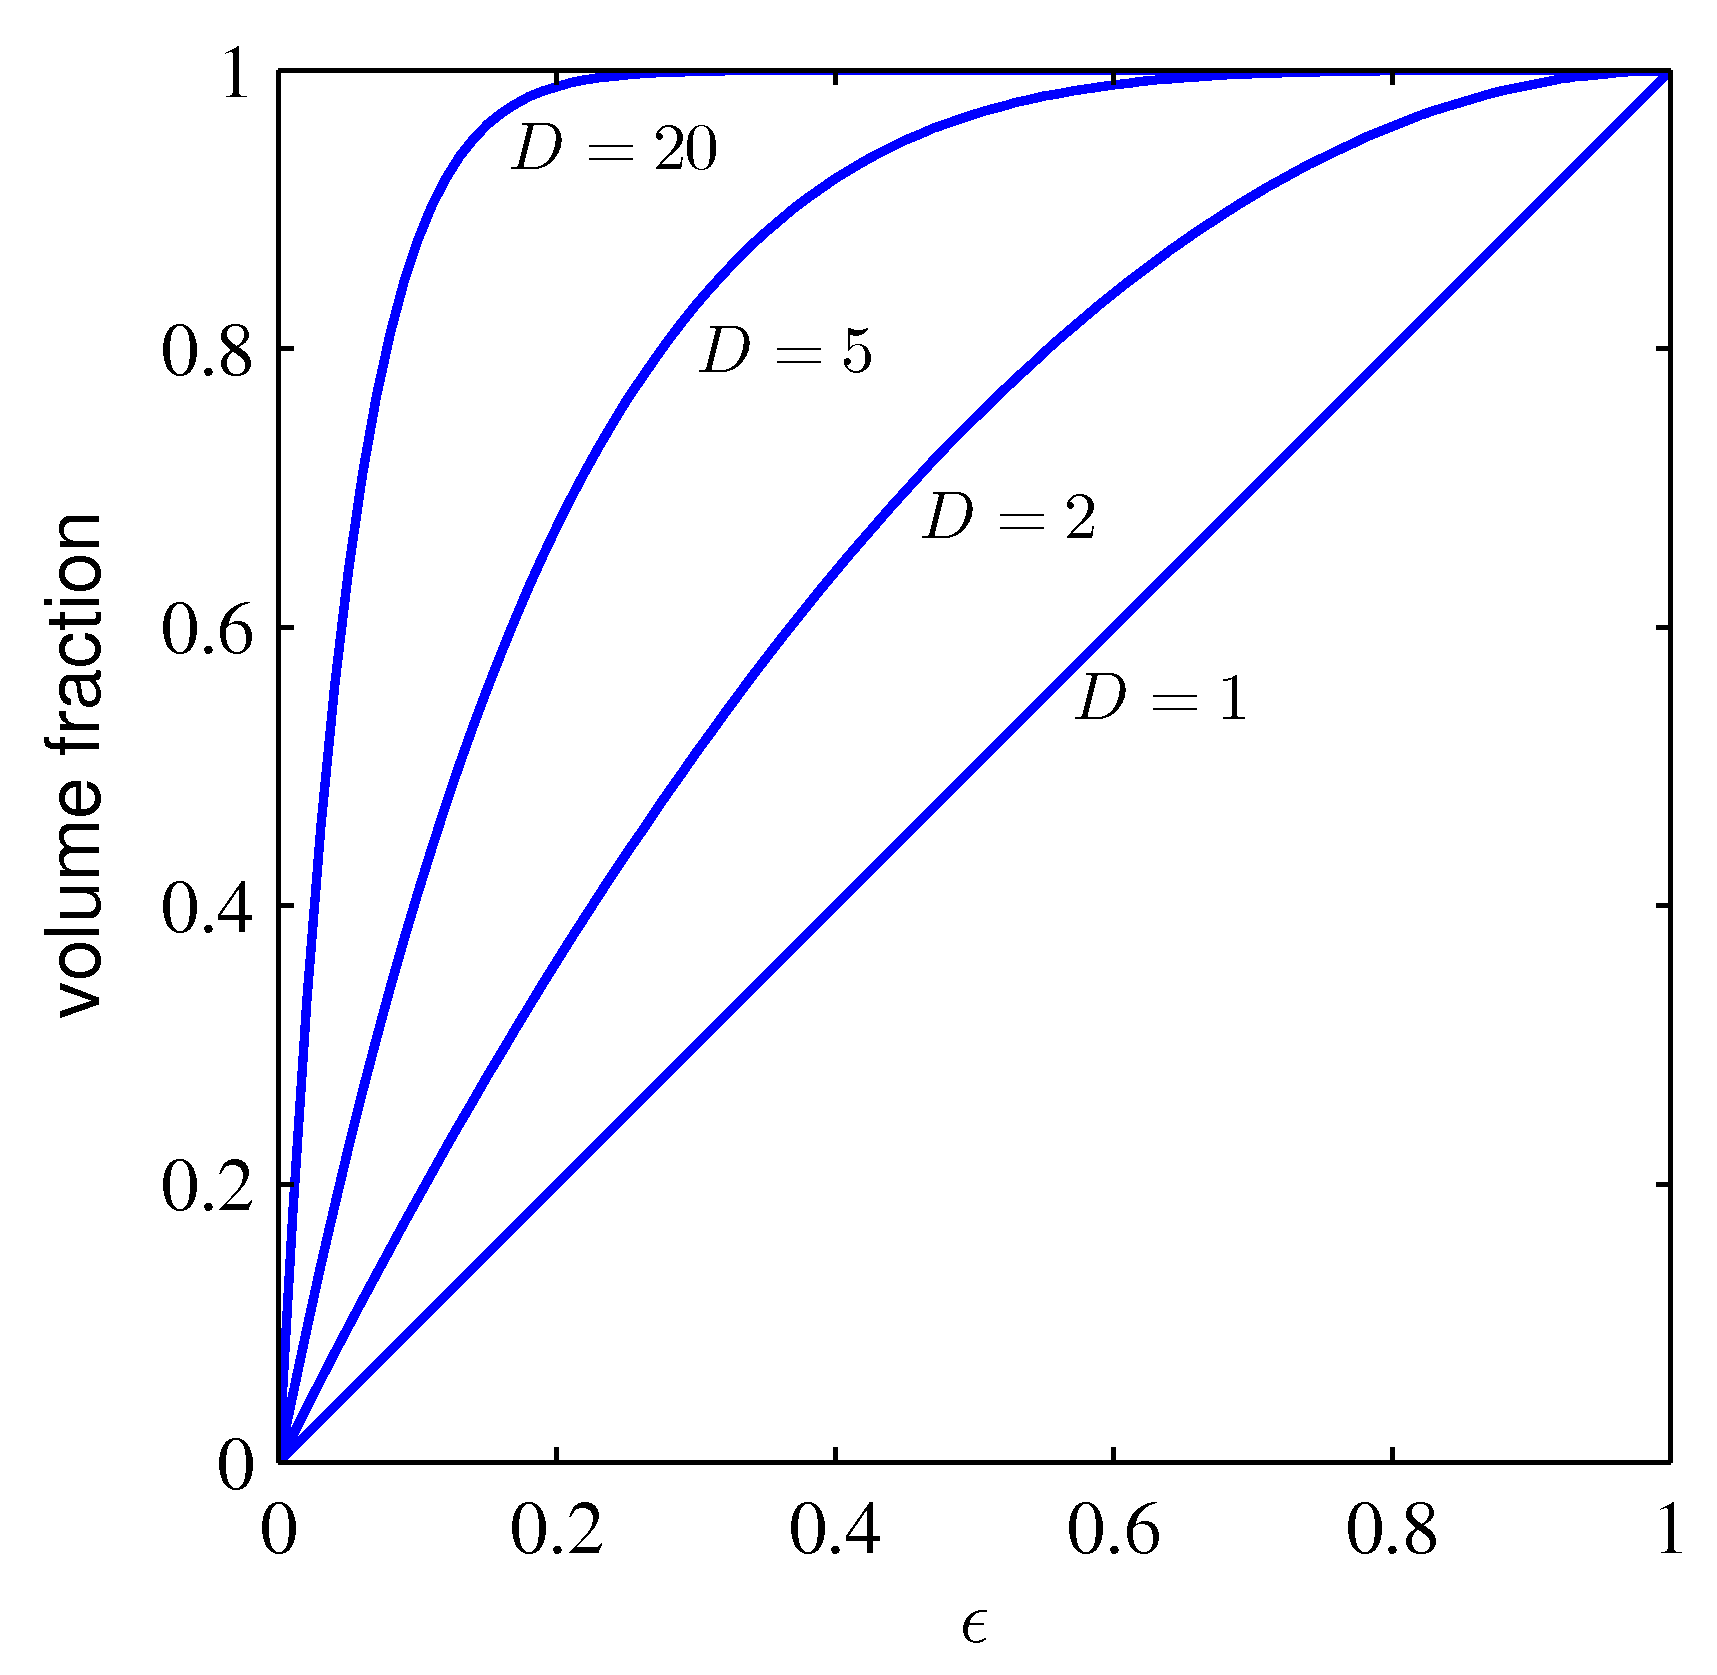
\includegraphics[scale=0.8]{Images/1-22.png}
		\captionsetup{font={small}}
		\caption{对于不同的$D$,球体中位于$r=1-\epsilon$与$r=1$之间的体积}
		\label{fig:1-22}
	\end{figure}
	\\
	\indent 作为与模式识别直接相关的另一示例,接下来研究一下高维空间中的高斯分布的特性。如果将笛卡尔坐标系变换为极坐标系,并对方向变量积分,就可以确定密度$p(r)$的表达式,$p(r)$是一个关于半径$r$的函数。所以$p(r)\delta r$就是位于$r$处厚度为$\delta r$的薄壳的概率质量。对于不同的$D$,分布的曲线如图1.23所示。我们可以看出对于较大的$D$,高斯分布的概率质量会集中在一个薄壳里。\color{red} \textbf{——习题 1.20} \color{black}
	\begin{figure}[ht]
		\centering
		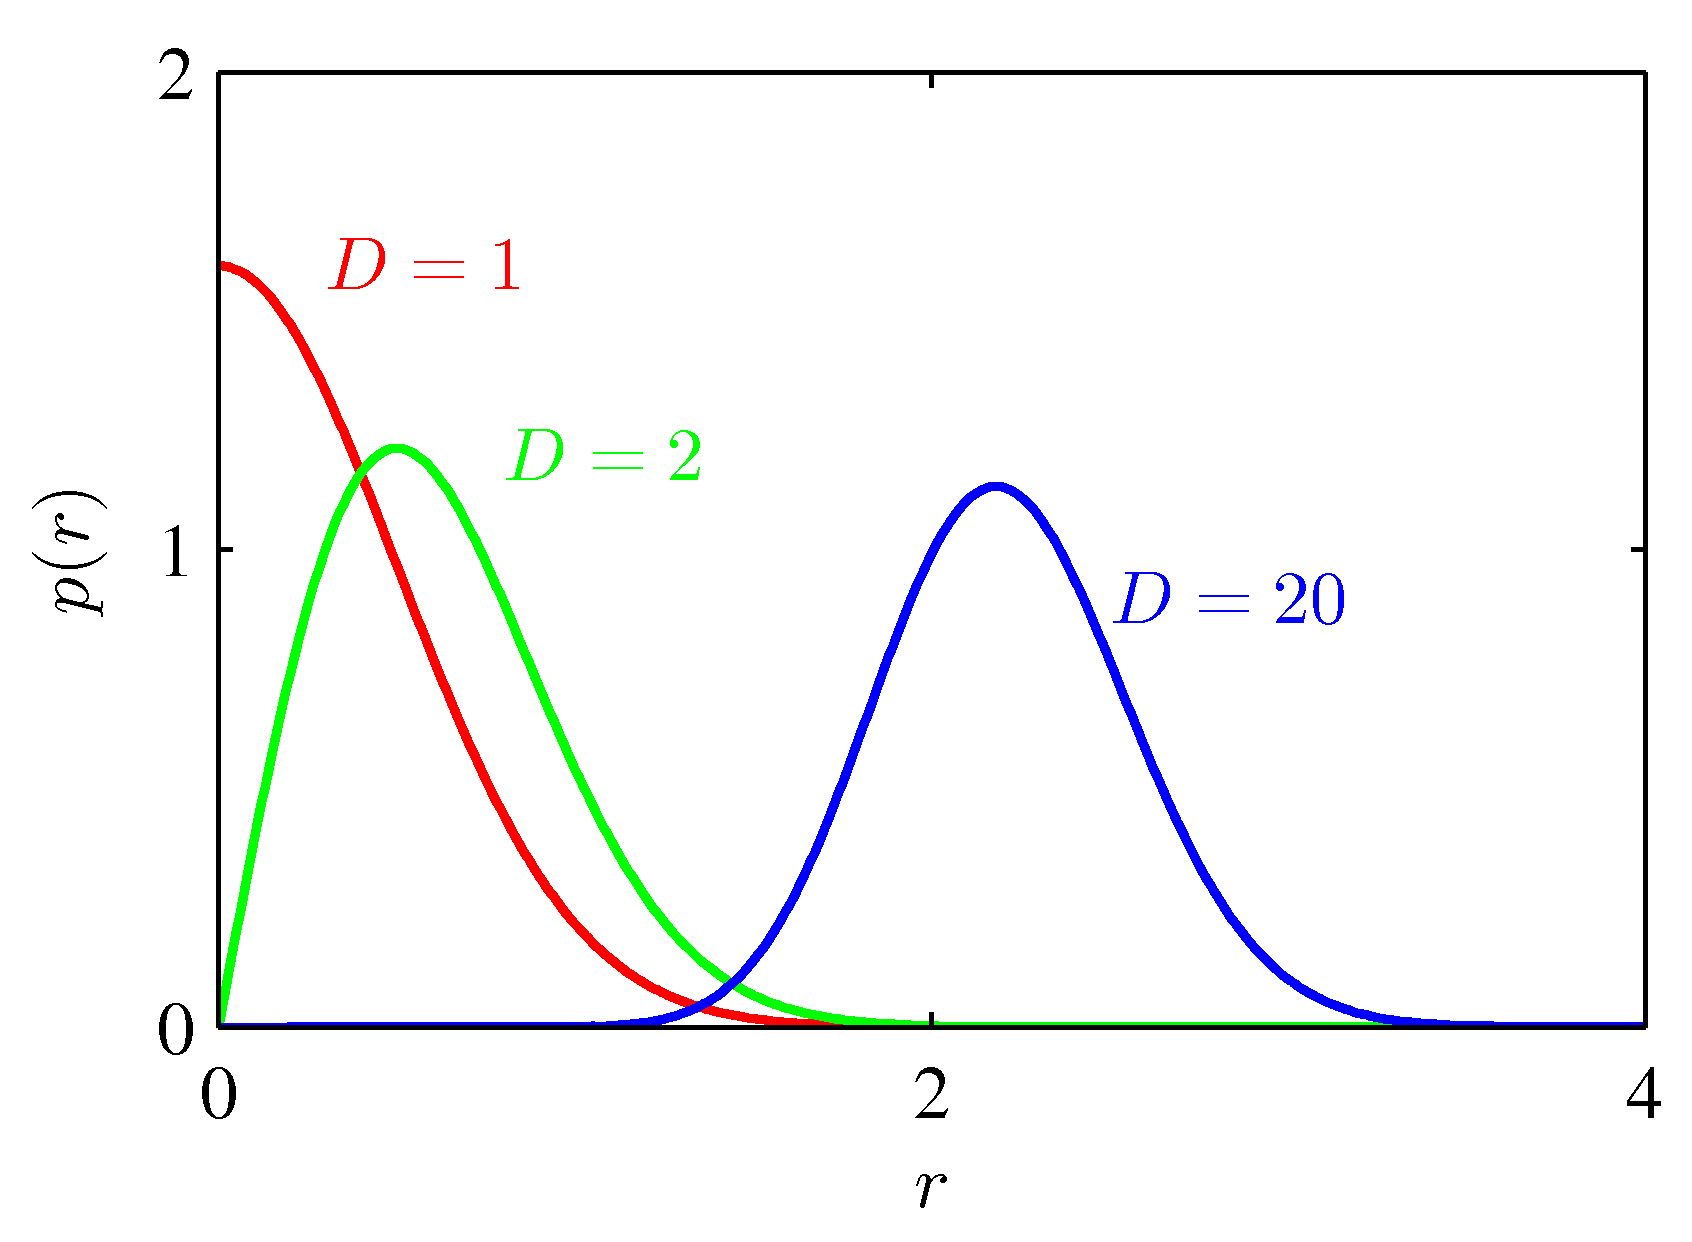
\includegraphics[scale=0.8]{Images/1-23.png}
		\captionsetup{font={small}}
		\caption{在维数$D$取不同值时关于$r$的高斯分布的概率密度。在高维的空间中,一个高斯分布的概率质量主要集中在特定半径位置的薄壳内。}
		\label{fig:1-23}
	\end{figure}
	\\
	\indent 这些可能在高维空间中出现的严重问题有时被称为维数灾难(curse of dimensionality, Bellman, 1961)。在本书中,我们会广泛使用输入空间为一维或二维空间中的例子,因为这样可以让各种图形表达更加清楚和简单。但读者应该留意,并非所有在低维空间中形成的习惯性直觉都可以推广到高维空间。\\
	\indent 尽管维数灾难确实是模式识别中的一个大麻烦,但这并不能阻止我们有效处理高维空间的问题。理由有两方面。首先,真实的数据往往都会被限制在较低有效维度的空间区域中,特别是在目标变量可能会发生重要变化的方向上。其次,真实的数据通常会表现出一些平滑性(至少在局部上),所以在大多数情况下,输入变量的微小变化也不会对目标变量产生太大的影响,因此可以使用类似于局部插值的方法对新的输入变量进行相应目标变量的预测。成功的模式识别技术一定会利用这些特性,要么利用其一,要么二者兼有。举例而言,让我们设想一种在生产制造中模式识别的应用,假设我们获取了某条传送带上某种特定平面物体的图像,要利用图像判断它们的方向。每张图像其实都是高维空间中的一个点,而这个高维空间的维度是由图像的像素数确定的。由于物体可能在图像中的任何位置出现,其方向也是随机的,所以图像之间存在3个可变自由度,而且这些图像会存在于高维空间中的一个三维流形(manifold)上。由于物体的位置和方向与像素强度之间的关系实在太复杂,这个流形会是高度非线性的。如果我们的目标改变为仅利用输入图像输出物体的方向,而不需要应对位置变化的问题,那么这个流形一下子就变成仅有1个可变自由度了。
	}
	\section{决策论}
	\noindent{\color{red} \rule[10pt]{\textwidth}{0.1em}}
	\textnormal{
	\indent 在1.2节中我们已经看到,概率论让我们可以利用这个连贯的数学框架来量化和控制不确定性。现在我们转向决策论的讨论,当决策论与概率论相结合,我们就可以有效应对含有不确定性的模式识别问题,并做出最优的决策。\\
	\indent 假设我们现在有一个输入向量$\boldsymbol{\mathrm{x}}$,它对应的目标向量是$\boldsymbol{\mathrm{t}}$,目标仍然是为新的$\boldsymbol{\mathrm{x}}$预测$\boldsymbol{\mathrm{t}}$。对于回归问题而言,$\boldsymbol{\mathrm{t}}$为连续变量,对于分类问题而言,$\boldsymbol{\mathrm{t}}$为类别标签。联合概率分布$p(\boldsymbol{\mathrm{x}},\boldsymbol{\mathrm{t}})$是对不确定性的完整概述,而不确定性是与变量密切相关的。利用训练数据集确定$p(\boldsymbol{\mathrm{x}},\boldsymbol{\mathrm{t}})$称为推断(inference),这个问题相当困难,以至于它的解决手段就构成了本书涉及到的很多学科。但是在实际应用中,对$\boldsymbol{\mathrm{t}}$做出具体的预测是不可避免的,而且更多的时候还要基于$\boldsymbol{\mathrm{t}}$的取值采取具体的行动,这就是决策论的研究内容。\\
	\indent 举例而言,假设我们现在有一个医学诊断问题,要通过病人的X光片来判断病人是否得了肿瘤。在这种情况下,输入向量$\boldsymbol{\mathrm{x}}$是来自图像的一系列像素强度,输出变量$t$表示肿瘤的存在与否,若肿瘤存在则分类为$\mathcal{C}_1$,反之为$\mathcal{C}_2$。我们可能会将$t$设定为二值变量,$t=0$对应类别$\mathcal{C}_1$,$t=1$对应类别$\mathcal{C}_2$。我们将在稍后看到这样取值对概率模型来说相当方便。这个推断问题接下来涉及到确定联合分布$p(\boldsymbol{\mathrm{x}},\mathcal{C}_k)$,或者其等价形式$p(\boldsymbol{\mathrm{x}},\boldsymbol{\mathrm{t}})$,从而给出这一问题的完整概率表述。尽管概率模型可以提供非常实用而且丰富的信息,但我们最终的目的还是确定这个患者是否需要治疗,而且我们当然希望做出的决策在某种意义上是最优的(Duda and Hart, 1973)。这就是决策(decision)步骤,而且决策论的主题就是告诉我们如何在给定了适当概率的情况下做出最优决策。我们将看到,一旦解决了推断问题,决策步骤就将是非常简单,甚至可以说是微不足道的。\\
	\indent 在这里我们会介绍一些本书后续内容要求掌握的决策论关键思想。对于更广泛的背景知识和更加详细的叙述,可以参考Berger(1985)和Bather(2000)的有关研究。\\
	\indent 在给出详细的分析之前,首先不太正式地研究一下概率论如何在决策中发挥重要的作用。当我们得到一个新病人的X光片$\boldsymbol{\mathrm{x}}$之后,我们要判定这张图像会指向两种结果中的哪一种。我们想要的是“给定图像的情况下结果分类的概率”,也就是$p(\mathcal{C}_k | \boldsymbol{\mathrm{x}})$。利用贝叶斯定理,这个概率可以表达为
	\begin{equation}
		p(\mathcal{C}_k | \boldsymbol{\mathrm{x}}) = \frac{p(\boldsymbol{\mathrm{x}}|\mathcal{C}_k)p(\mathcal{C}_k)}{p(\boldsymbol{\mathrm{x}})}
	\end{equation}
	需要注意的是,在贝叶斯定理中出现的任何值都可以利用联合分布$p(\boldsymbol{\mathrm{x}},\mathcal{C}_k)$对适当变量进行边缘化或条件化来得到。现在我们可以将$p(\mathcal{C}_k)$解释为类别$\mathcal{C}_k$的先验概率,将$p(\mathcal{C}_k | \boldsymbol{\mathrm{x}})$解释为对应的后验概率。因此,$p(\mathcal{C}_1)$表示在进行X光检测之前病人患有肿瘤的先验概率。类似地,$p(\mathcal{C}_1 | \boldsymbol{\mathrm{x}})$是其对应的后验概率,表示拿到X光检测结果之后利用其中的信息和贝叶斯定理对患有肿瘤的概率进行了修正。如果我们的目标是将$\boldsymbol{\mathrm{x}}$分类错误的可能性最小化,那么直觉上我们应当选择具有更高后验概率的那个类别。现在我们证明这个直觉是正确的,并讨论做决策的更加一般的标准。}
	\subsection{分类误差最小化}
	\textnormal{现在先假设我们的目标仅仅是要尽可能不出现分类错误的情况。为了给每个输入向量$\boldsymbol{\mathrm{x}}$分配一个合理的类别,我们肯定是需要依赖于一定的规则的。这样的规则会将整个输入空间分割成不同的区域$\mathcal{R}_k$,也就是决策域(decision regions),而且每个类别都对应一个决策域,于是$\mathcal{R}_k$中所有的点就都被分配了类别$\mathcal{C}_k$。决策域之间的边界被称为决策界(decision boundaries)或者决策面(decision surfaces)。需要注意的是,决策域并不一定是连在一起的,不相邻的区域也可以属于同一个决策域。我们会在后面的章节中讨论决策域和决策界的例子。在这里首先考虑二分类中寻找最优决策规则的问题,比如之前提及到的那个肿瘤诊断的例子,如果将一个实际上属于类别$\mathcal{C}_1$的输入分到了$\mathcal{C}_2$,那肯定是大错特错了,反过来也是一样。这种情况出现的概率可以表示为
	\begin{equation}
		\begin{split}
			p(\mathrm{mistake})&=p(\boldsymbol{\mathrm{x}}\in \mathcal{R}_1,\mathcal{C}_2) + p(\boldsymbol{\mathrm{x}}\in \mathcal{R}_2,\mathcal{C}_1) \\
			&=\int_{\mathcal{R}_1}p(\boldsymbol{\mathrm{x}},\mathcal{C}_2) \ \mathrm{d}\boldsymbol{\mathrm{x}} + \int_{\mathcal{R}_2}p(\boldsymbol{\mathrm{x}},\mathcal{C}_1) \ \mathrm{d}\boldsymbol{\mathrm{x}}
		\end{split}
	\end{equation}
	\indent 根据决策规则可以给每个$\boldsymbol{\mathrm{x}}$分配两种类别中的一个,而且这个决策规则是我们自行选择的。很明显,为了让$p(\mathrm{mistake})$尽可能地小,那么将$\boldsymbol{\mathrm{x}}$分配到哪种类别能让(1.78)中的积分式最小,就应该将其分到哪种类别。所以,如果$p(\boldsymbol{\mathrm{x}},\mathcal{C}_1)>p(\boldsymbol{\mathrm{x}},\mathcal{C}_2)$,那就应该把$\boldsymbol{\mathrm{x}}$归类到$\mathcal{C}_1$。根据概率论的乘法规则,我们有$p(\boldsymbol{\mathrm{x}},\mathcal{C}_k)=p(\mathcal{C}_k|\boldsymbol{\mathrm{x}})p(\boldsymbol{\mathrm{x}})$。由于两个积分项中的$p(\boldsymbol{\mathrm{x}})$是一样的,所以实际上那个初始的问题就可以转化为,对每个$\boldsymbol{\mathrm{x}}$分配一个使得后验概率$p(\mathcal{C}_k|\boldsymbol{\mathrm{x}})$最大的类别。图1.24所示的就是对于一个一元输入变量$x$进行二分类的问题。
	\begin{figure}[ht]
		\centering
		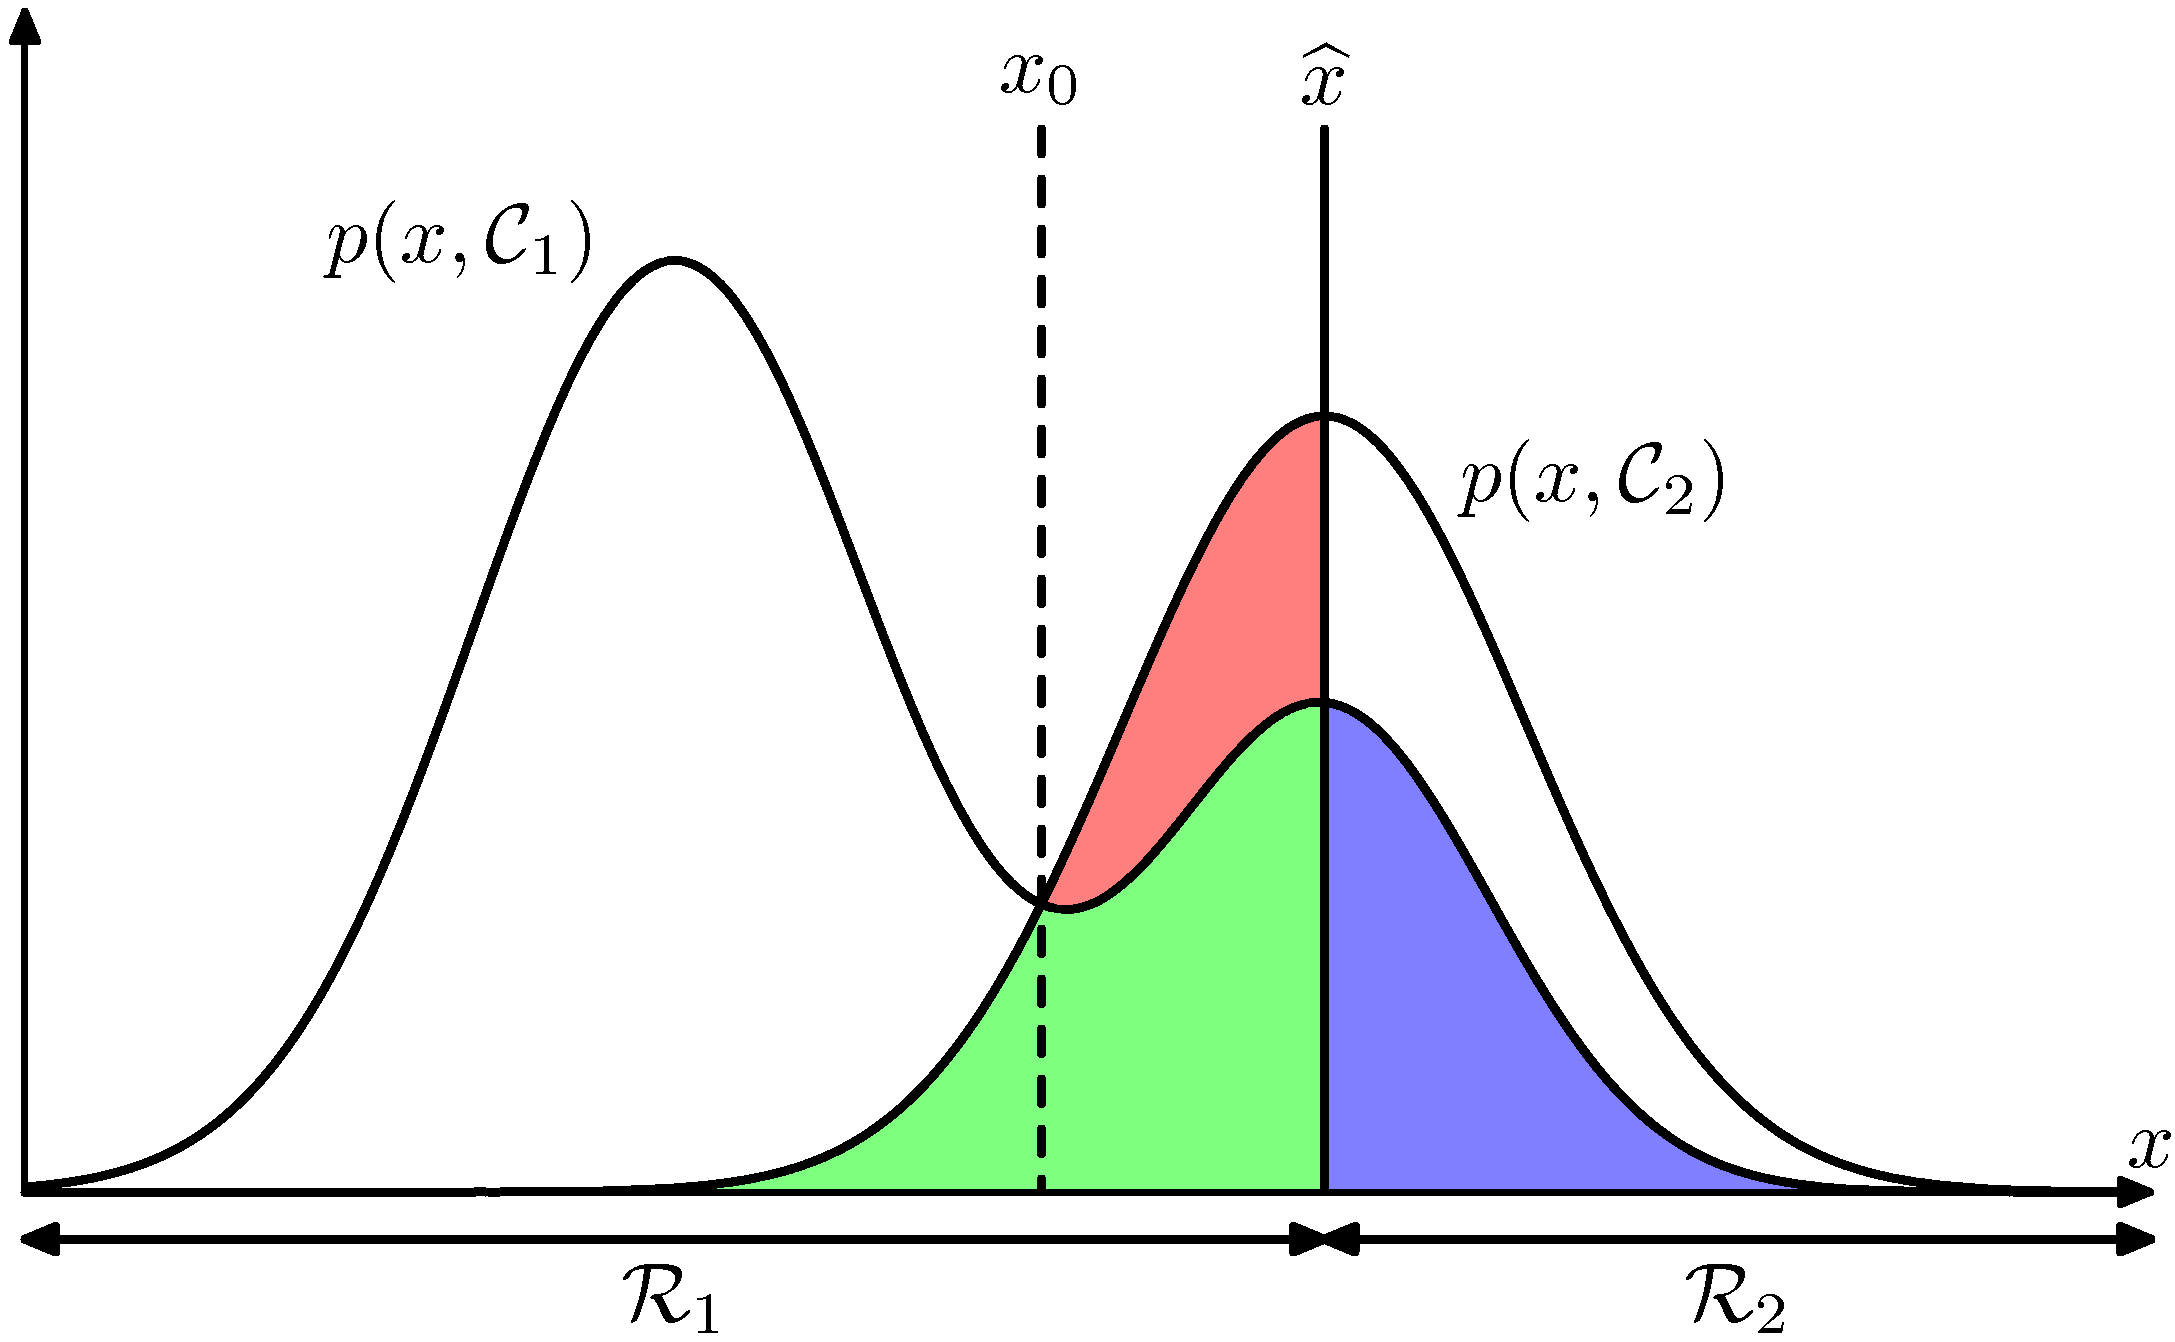
\includegraphics[scale=0.8]{Images/1-24.png}
		\captionsetup{font={small}}
		\caption{在二分类问题中两种类别分别关于$x$的联合概率$p(x,\mathcal{C}_k)$,同时指出了决策界$x=\hat{x}$的示意图。若$x \geqslant \hat{x}$则分类为$\mathcal{C}_2$,所以是属于决策域$\mathcal{R}_2$的,反过来,如果$x < \hat{x}$则分类为$\mathcal{C}_1$,属于决策域$\mathcal{R}_1$。分类错误来源于蓝色、绿色和红色区域,在$x < \hat{x}$的情况中,产生的错误主要是将本属于$\mathcal{C}_2$的$x$分类成$\mathcal{C}_1$,也就是红色区域和绿色区域的总和;反过来,在$x \geqslant \hat{x}$的情况中,产生的错误主要是将本属于$\mathcal{C}_1$的$x$分类成$\mathcal{C}_2$,也就是蓝色区域了。当我们改变决策域$\hat{x}$的位置,由于绿色区域和蓝色区域连在一起,它们的总和是不变的,而红色区域的大小是会发生变化的。决策域$\hat{x}$的最佳选择,应该是两条曲线$p(x,\mathcal{C}_1)$和$p(x,\mathcal{C}_2)$的相交处,也就是图中$x_0$的位置,因为在这里,红色区域就完全消失了。对于分类误差最小化问题的决策规则也是这样,实质上就是要将$x$归类于后验概率$p(\mathcal{C}_k|x)$更高的那一类。}
		\label{fig:1-24}
	\end{figure}
	\\
	\indent 对于更加一般的$K$分类问题,写成正确概率最大化的形式会更简单一些,也就是
	\begin{equation}
		\begin{split}
			p(\mathrm{correct})&=\sum_{k=1}^{K}p(\boldsymbol{\mathrm{x}}\in \mathcal{R}_k,\mathcal{C}_k)\\
			&=\sum_{k=1}^{K}\int_{\mathcal{R}_k}p(\boldsymbol{\mathrm{x}},\mathcal{C}_k)\ \mathrm{d}\boldsymbol{\mathrm{x}}
		\end{split}	
	\end{equation}
	这项概率会在$\boldsymbol{\mathrm{x}}$分配到使得$p(\boldsymbol{\mathrm{x}},\mathcal{C}_k)$取得最大值的决策域时达到最大值。再次利用乘法规则$p(\boldsymbol{\mathrm{x}},\mathcal{C}_k)=p(\mathcal{C}_k|\boldsymbol{\mathrm{x}})p(\boldsymbol{\mathrm{x}})$,并且再次留意到对于每个积分项来说$p(\boldsymbol{\mathrm{x}})$都是相同的,我们发现$\boldsymbol{\mathrm{x}}$应该分类到具有最大后验概率$p(\mathcal{C}_k|\boldsymbol{\mathrm{x}})$的类别。
	}
	\subsection{期望损失最小化}
	\textnormal{在很多的应用中,我们的目标不仅仅是将分类误差进行最小化,而往往是要更复杂一些。还是回到之前那个肿瘤诊断的问题,我们注意到,如果一个没有肿瘤的病人被误诊为患有肿瘤,那么会给病人带来无端的痛苦和后续的进一步诊断。而反过来,如果一个患有肿瘤的病人被认为是没有患病,那可能会导致病人没有得到及时的治疗最后翘辫子。很明显,比起第一种,第二种错误造成的后果要更加严重,所以宁可让第一种错误多犯一些,也要削减第二种错误出现的可能性。\\
	\indent 我们可以将这个问题写成损失函数(loss function)或者叫做代价函数(cost function)的形式。损失函数,是衡量在决策中采取任何一种决策或行动而造成的损失的单值标准。我们的目标是尽可能地减少总体损失。不过在其他的研究中,一些研究人员将这个问题视为效益函数(utility function)最大化的问题,其实和损失函数最小化是等价的,只需将损失取相反数就可以了,现在我们采用的是损失函数的形式。对于一个新的$\boldsymbol{\mathrm{x}}$,假设其真实类别是$\mathcal{C}_k$,而我们将其分类为$\mathcal{C}_j$——$j$可能等于$k$,也可能不等于$k$。这样做的结果,就是造成了损失$L_{kj}$,这个损失可以被看成是损失矩阵(loss matrix)中的$(k,j)$元素。举例而言,在肿瘤诊断的例子中,我们可以将损失矩阵设置成如图1.25所示的形式。这个损失矩阵表示的是,在分类正确的时候不会造成任何损失,如果将健康病人误诊为患有肿瘤,那么损失是1,而如果将一个患有肿瘤的病人误诊为健康,那么损失就是1000。
	\begin{figure}[ht]
		\centering
		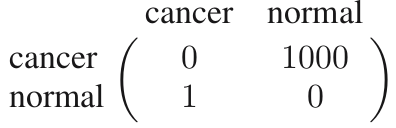
\includegraphics[scale=0.25]{Images/1-25.png}
		\captionsetup{font={small}}
		\caption{肿瘤诊断问题中的损失矩阵示例。每一行表示真实类别,每一列表示根据决策规则得出的分类结果。}
		\label{fig:1-25}
	\end{figure}
	\\
	\indent 最佳的解决方案,就是让损失函数最小的那一种。然而,损失函数是与真实类别有关的,而真实类别往往却是未知的。对于给定的输入变量$\boldsymbol{\mathrm{x}}$,其真实类别的不确定性是通过联合概率分布$p(\boldsymbol{\mathrm{x}},\mathcal{C}_k)$来表示的,所以我们需要一个替代方案,求取平均损失,而这个平均损失是根据联合概率分布求得的,可以表示为
	\begin{equation}
		\mathbb{E}[L]=\sum_k \sum_j \int_{\mathcal{R}_j}L_{kj}p(\boldsymbol{\mathrm{x}},\mathcal{C}_k)\ \mathrm{d}\boldsymbol{\mathrm{x}}
	\end{equation}
	任意的$\boldsymbol{\mathrm{x}}$都可以被指派到决策域之一$\mathcal{R}_j$中。我们的任务就是选择合适的$\mathcal{R}_j$,从而使得(1.80)中的期望损失最小,也就是说对于任意的$\boldsymbol{\mathrm{x}}$我们需要将$\sum_k L_{kj}p(\boldsymbol{\mathrm{x}},\mathcal{C}_k)$进行最小化。和往常一样,这里也可以用乘法规则$p(\boldsymbol{\mathrm{x}},\mathcal{C}_k)=p(\mathcal{C}_k|\boldsymbol{\mathrm{x}})p(\boldsymbol{\mathrm{x}})$,然后省略掉共同的因子$p(\boldsymbol{\mathrm{x}})$。所以使得期望损失最小的决策规则就是,给每个新的$\boldsymbol{\mathrm{x}}$分配的类别$j$应当使
	\begin{equation}
		\sum_k L_{kj}p(\mathcal{C}_k|\boldsymbol{\mathrm{x}})
	\end{equation}
	最小化。一旦我们知道了后验分类概率$p(\mathcal{C}_k|\boldsymbol{\mathrm{x}})$,这个问题就是轻而易举的了。
	}
	\subsection{拒绝选项}
	\textnormal{我们已经看到分类误差源自于输入空间中这样的一些区域中——区域中最大的后验概率$p(\mathcal{C}_k|\boldsymbol{\mathrm{x}})$明显低于整体水平,或者等价地说,区域中各个联合分布$p(\boldsymbol{\mathrm{x}},\mathcal{C}_k)$的值比较势均力敌。在这些区域里,该怎样进行分类是比较让人头疼的一件事。在实际应用中,为了让错误率低一些,比较明智的做法是直接逃避,避免在这些容易导致分类错误的样例上做决策,所谓“君子不立于危墙之下”,这就是拒绝选项(reject option)。比如说,在肿瘤诊断的问题中,可以利用一个自动分类系统,将诊断结果可能存在疑问的那些X光片挑选出来,再由专家进行人工的判断,从而得到更加准确的结果。我们可以通过设定一个阈值$\theta$来实现这项功能,将最大后验概率$p(\mathcal{C}_k|\boldsymbol{\mathrm{x}})$低于或等于$\theta$的输入$\boldsymbol{\mathrm{x}}$全部拒绝掉。图1.26所示是对于一个一元输入变量$x$进行二分类的示例。需要注意的是,将阈值设置为$\theta =1$就是将全部输入样例都拒绝掉,同时,对于$K$分类问题,将阈值设置为$\theta < 1/K$就是不拒绝任何输入样例了。所以输入样例中被拒绝的比例取决于$\theta$的值。
	\begin{figure}[ht]
		\centering
		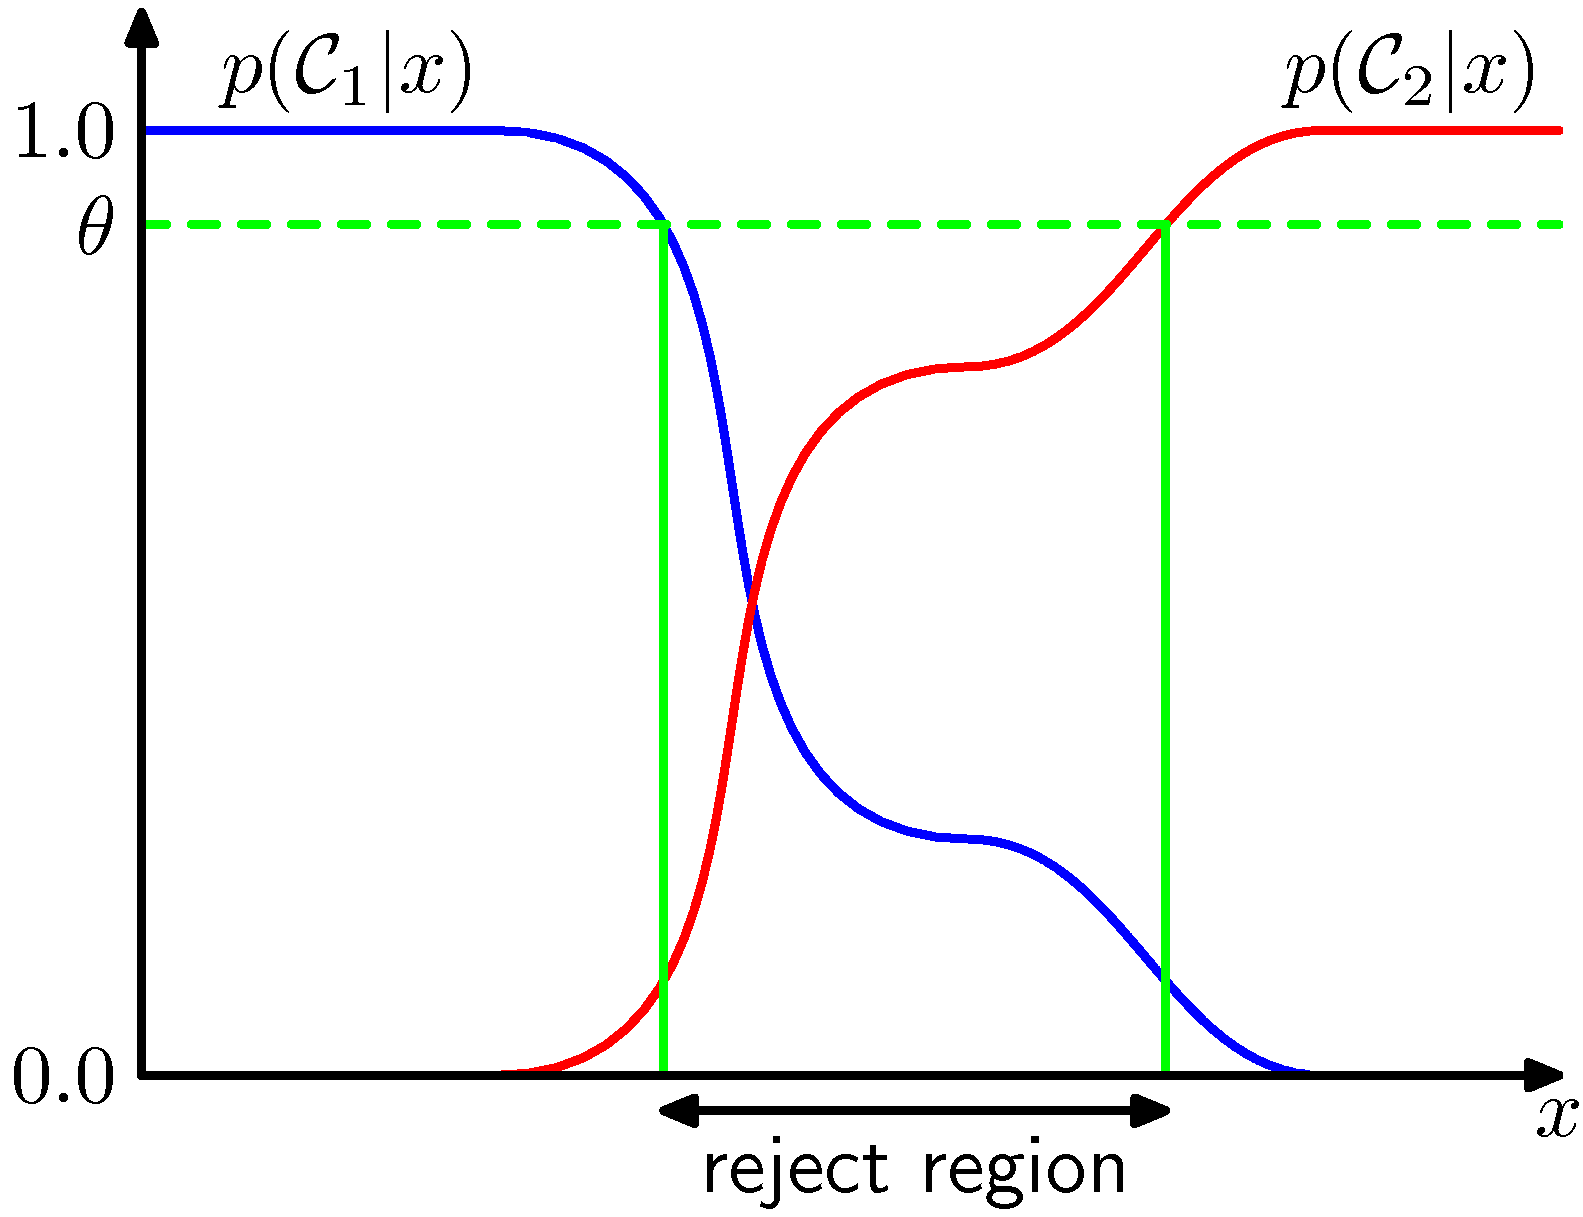
\includegraphics[scale=0.8]{Images/1-26.png}
		\captionsetup{font={small}}
		\caption{拒绝选项示意图。当两个后验概率中的最大值小于或等于某个阈值$\theta$时,这个输入$x$就会被拒绝。}
		\label{fig:1-26}
	\end{figure}
	\\
	\indent 当损失矩阵已知的情况下,我们可以很轻松地将拒绝选项引到期望误差最小化中,从而考虑做出拒绝的决定时造成的损失。\color{red} \textbf{——习题 1.24} \color{black}}
	\subsection{推断与决策}
	\textnormal{我们已经将分类问题拆分成两个步骤,在推断步骤(inference stage),我们利用训练数据来学习一个$p(\mathcal{C}_k|\boldsymbol{\mathrm{x}})$的模型,而在后续的决策步骤(decision stage),我们会利用这些后验概率来进行最优的分类。一个二选一的概率可以将这两个问题一同解决,只需要学习一个直接将输入$\boldsymbol{\mathrm{x}}$指向决策结果的函数就可以了。这样的函数被称为判别函数(discriminant function)。\\
	\indent 实际上,解决决策问题有三种不同的方法,它们都可以用于实际应用中,而且我们可以明确地辨认它们。根据复杂程度降序排列,这些方法分别是:\\
	\textbf{(a)}\ 首先解决推断问题,也就是确定分类——对于每一种类别$\mathcal{C}_k$求取条件概率密度$p(\boldsymbol{\mathrm{x}}|\mathcal{C}_k)$。同时还要分别确定分类先验概率$p(\mathcal{C}_k)$。然后采用如下形式的贝叶斯定理
	\begin{equation}
		p(\mathcal{C}_k|\boldsymbol{\mathrm{x}})=\frac{p(\boldsymbol{\mathrm{x}}|\mathcal{C}_k)p(\mathcal{C}_k)}{p(\boldsymbol{\mathrm{x}})}
	\end{equation}
	来求取分类后验概率$p(\mathcal{C}_k|\boldsymbol{\mathrm{x}})$。和往常一样,贝叶斯定理中的分母可以写成分子求和的形式,因为
	\begin{equation}
		p(\boldsymbol{\mathrm{x}})=\sum_k p(\boldsymbol{\mathrm{x}}|\mathcal{C}_k)p(\mathcal{C}_k)
	\end{equation}
	等价地,我们也可以直接建立联合分布$p(\boldsymbol{\mathrm{x}},\mathcal{C}_k)$,然后进行归一化,以得到后验概率。得到后验概率之后,利用决策论来确定每个新的输入$\boldsymbol{\mathrm{x}}$的分类。或明确或隐含地对输入和输出进行建模的方法被称为生成模型(generative models),因为通过在其中采样就可以在输入空间生成数据点。\\
	\textbf{(b)}\ 首先解决推断问题,但先确定后验分类概率$p(\mathcal{C}_k|\boldsymbol{\mathrm{x}})$,然后利用决策论,为每个新的$\boldsymbol{\mathrm{x}}$进行分类。这种直接利用后验概率的方法称为判别模型(discriminative models)。\\
	\textbf{(c)}\ 寻找将输入$\boldsymbol{\mathrm{x}}$直接映射到分类标签的判别函数$f(\boldsymbol{\mathrm{x}})$。举例而言,在二分类问题中,$f(\cdot)$应该是一个二值函数,$f=0$表示类别$\mathcal{C}_1$,$f=1$表示类别$\mathcal{C}_2$。在这种情况中,概率论没有发挥作用。\\
	\indent 接下来研究这三种方法各自的优点。方法(a)是要求最多的,因为要找到$\boldsymbol{\mathrm{x}}$和$\mathcal{C}_k$的联合分布。在很多实际应用中,$\boldsymbol{\mathrm{x}}$的维度可能是很高的,所以我们可能需要很大的训练集来保证分类的条件概率密度函数是充分准确的。需要注意的是,分类先验$p(\mathcal{C}_k)$通常可以比较简单地利用训练数据中属于各个分类的样本比例进行估计。但方法(a)的一大优点,就是可以利用(1.83)确定数据的边缘概率密度$p(\boldsymbol{\mathrm{x}})$。这对于在模型下概率较低的和预测准确率较低的新数据是相当有用的,这个过程称为离群点检测(outlier detection) 或称为异常检测(novelty detection)(Bishop, 1994;Tarassenko, 1995)。\\
	\indent 然而,如果我们仅仅希望做出分类决策,那方法(a)中求取$p(\boldsymbol{\mathrm{x}},\mathcal{C}_k)$就很浪费计算资源了,而且对数据数量的要求太高,毕竟夯不啷当算了一大堆,其实用得上的只不过是$p(\mathcal{C}_k|\boldsymbol{\mathrm{x}})$而已,这种时候用方法(b)就直接得多了。毕竟分类的条件概率密度可能包含了一大堆对于后验概率没什么作用的内容,如图1.27所示。顺便一提,人们一直在探索机器学习中生成模型方法和判别模型方法各自的优点,而且对将两种方法结合起来的办法一直很感兴趣(Jebara, 2004; Lasserre et al., 2006)。
	\begin{figure}[ht]
		\begin{minipage}[t]{0.5\linewidth}
		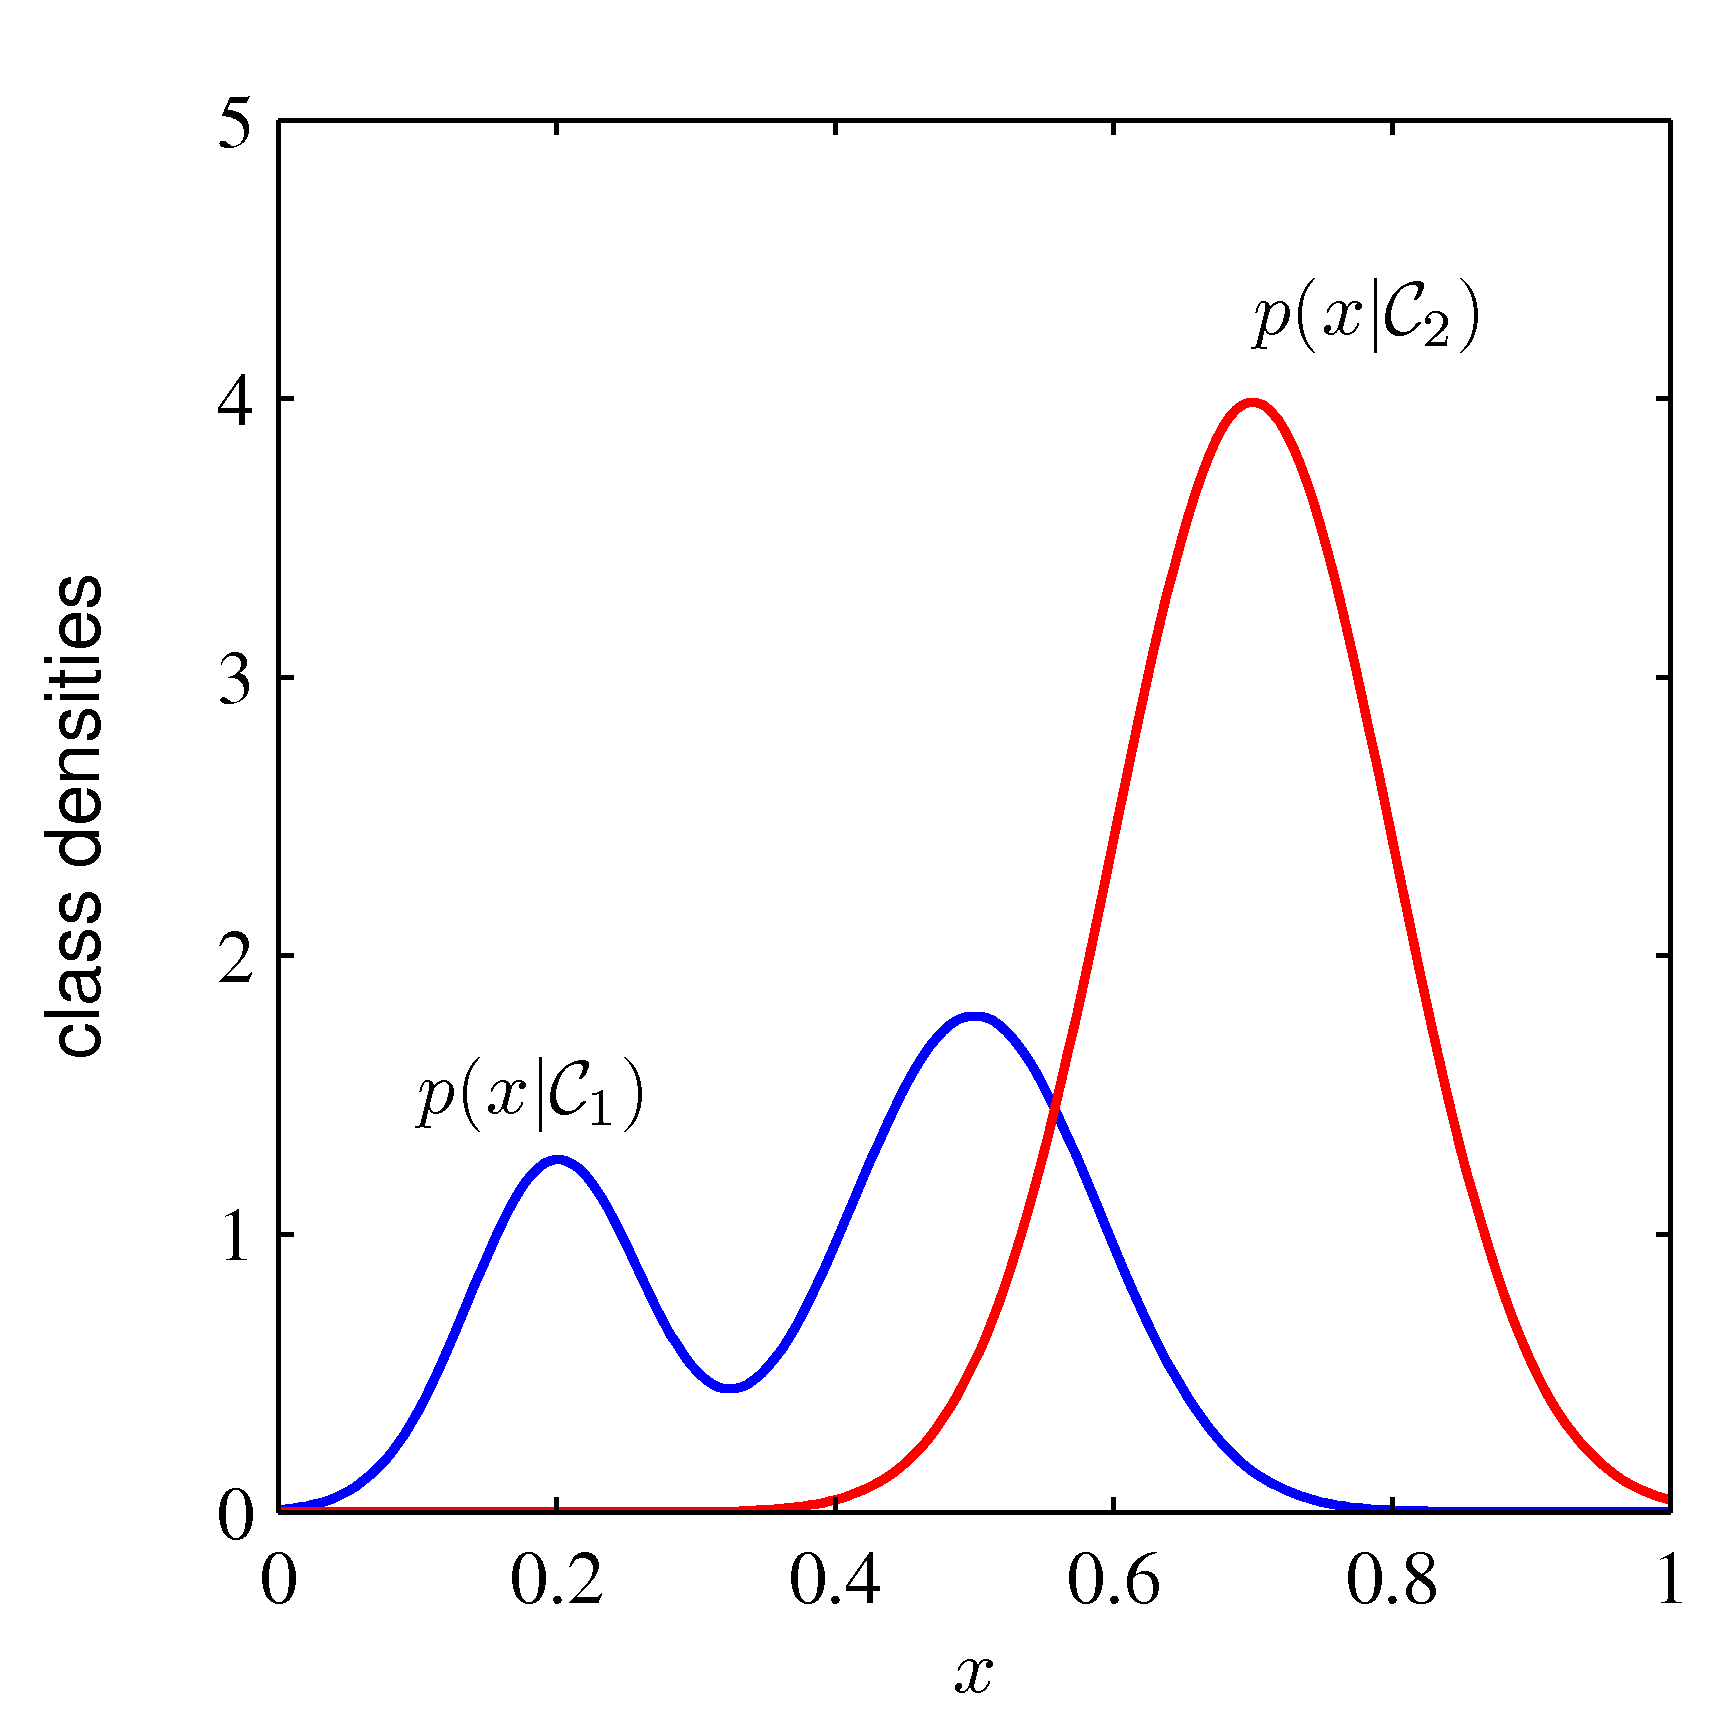
\includegraphics[scale=0.8]{Images/1-27a.png}
		\label{fig:1-27a}
		\end{minipage}
		\begin{minipage}[t]{0.5\linewidth}
		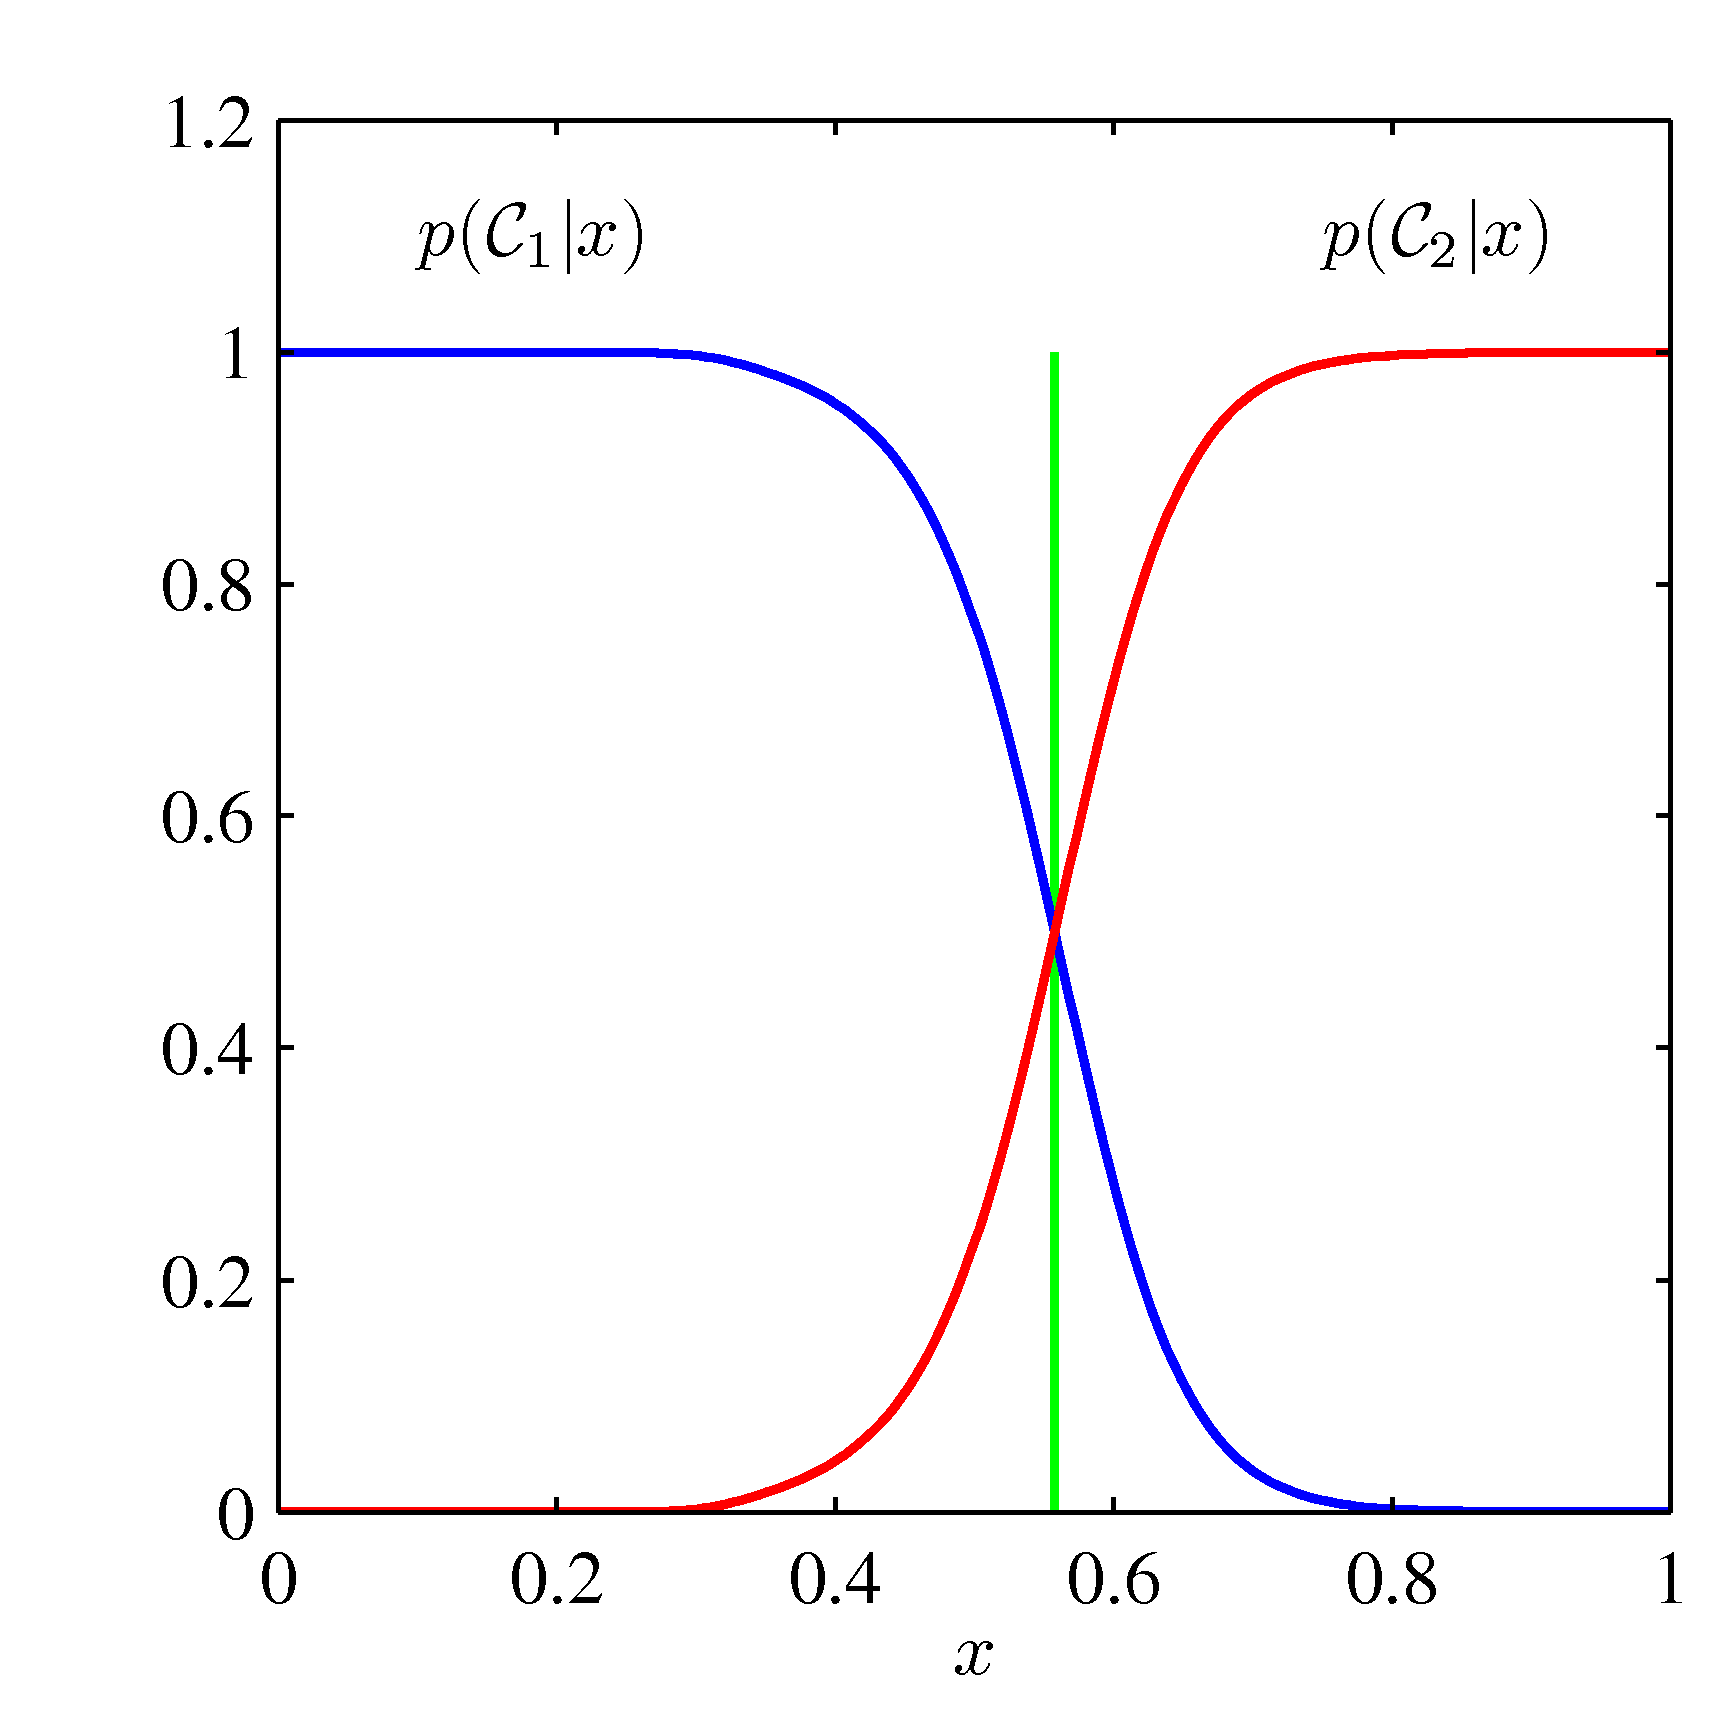
\includegraphics[scale=0.8]{Images/1-27b.png}
		\label{fig:1-27b}
		\end{minipage} 
		\captionsetup{font={small}}
		\caption{对一元输入变量$x$进行两种分类的条件概率密度(左图)和对应的后验概率(右图)。需要注意的是,左图中表示为蓝色曲线的分类条件概率密度$p(\boldsymbol{\mathrm{x}}|\mathcal{C}_k)$对于后验概率没有影响。右图中垂直的绿线表示的是假设分类的先验概率$p(\mathcal{C}_1)$和$p(\mathcal{C}_2)$相等的情况下,关于$x$的使得分类误差率最小的决策界。}
	\end{figure}
	\\
	\indent 方法(c)就更加简单了,只需要寻找分类函数$f(\boldsymbol{\mathrm{x}})$,将$\boldsymbol{\mathrm{x}}$映射到某种类别标签,于是就将推断和决策步骤结合成单一的学习问题了。如图1.27中的示例所示,这个方法是要找出垂直绿线对应的$x$值,因为这就是使得错误分类概率最小的决策界。\\
	\indent 但是,方法(c)会让我们无从获得后验概率$p(\mathcal{C}_k|\boldsymbol{\mathrm{x}})$。然而后验概率又是很必要的,即使是在后面做决策的时候都是很有用处的。理由包括:\\
	\indent \textbf{风险最小化。}让我们考虑这样的一个问题——损失矩阵里的元素会时刻发生变化,这种情况可能会出现在金融领域的应用中。如果我们知道后验概率,就可以轻而易举地通过修改(1.81)来修改决策标准,从而使风险最小化。如果我们只有判定函数,那么一旦损失矩阵发生任何变化,我们就必须重新进行训练,从头开始解决这个分类的问题。\\
	\indent \textbf{拒绝选项。}后验概率使得我们可以根据拒绝数据点的数量确定一个拒绝的标准,从而降低分类的错误率和减小期望损失。\\
	\indent \textbf{补偿分类先验。}还是拿X光诊断的问题说事。假设我们已经从公众群体中拿到了一个很大的X光片数据集来作为训练数据,从而构建一个自动诊断系统。由于在公众中肿瘤还是比较少见的,我们可能会发现1000例数据中才有1例是有肿瘤表现的。如果我们用这样的数据集去训练模型,由于患肿瘤的样本实在太少了,训练会遇到很多超级大麻烦。比如说,可能会得到一个将所有的输入数据都判定为属于未患病类别的分类器,而且还是有着99.9\% 准确率的那种,而且这种明显不对的结果还特别难以回避。另外,即使是很大的数据集也不会有多少样例是患有肿瘤的,所以学习算法的学习范围太狭窄了,不会有很好的泛化能力。只有那种各类样例数量差不多的,比较均衡的数据集才能够训练出准确的模型。然而如果这样做的话,就需要对训练数据的修正进行补偿。假设我们用这样经过修正的数据集得到了后验概率,根据贝叶斯定理(1.82),可以看出后验概率是与先验概率成比例的,而先验概率实际上就是每种类别的数据所占的比例。所以我们就可以利用从人工均衡过的数据集得到的后验概率,首先除以数据集中的类别比例,再乘以我们希望应用模型的公众中的类别比例。最后还需要对新得到的后验概率进行正则化,确保其总和为1。如果是直接学习了判别函数而不考虑后验概率的话,这个过程就不能进行了。\\
	\indent \textbf{联合模型。}对于复杂的应用来说,我们可能希望把问题拆分成很多小一点的子问题,每个子问题都当成是一个独立的单元来处理。比如之前那个诊断的问题,没准除了X光片我们还有其他的检测结果,比如说验血之类的。把这些内容全部整合到一个超巨型的输入空间,那这个问题就没法做了。所以还是分别对待比较明智,一个模型处理X光片,一个模型处理验血结果。两个模型分别给出了各个类别的后验概率,我们利用概率论中的定理直接就可以将它们的输出整合起来。比较简单的方法就是,假设对于各个类别,X光片的输入$\boldsymbol{\mathrm{x}}_\mathrm{I}$和验血的输入$\boldsymbol{\mathrm{x}}_\mathrm{B}$是相互独立的,也就是说
	\begin{equation}
		p(\boldsymbol{\mathrm{x}}_\mathrm{I},\boldsymbol{\mathrm{x}}_\mathrm{B}|\mathcal{C}_k)=p(\boldsymbol{\mathrm{x}}_\mathrm{I}|\mathcal{C}_k)p(\boldsymbol{\mathrm{x}}_\mathrm{B}|\mathcal{C}_k)
	\end{equation}
	这是条件独立(conditional independence)的一个例子,\color{red} \textbf{——第8.2节} \color{black}因为在给定类别$\mathcal{C}_k$的情况下,两个分布是相互独立的。X光片和验血结果共同给出的后验概率可以写成
	\begin{equation}
	\begin{split}
		p(\mathcal{C}_k|\boldsymbol{\mathrm{x}}_\mathrm{I},\boldsymbol{\mathrm{x}}_\mathrm{B}) &\propto p(\boldsymbol{\mathrm{x}}_\mathrm{I},\boldsymbol{\mathrm{x}}_\mathrm{B}|\mathcal{C}_k)p(\mathcal{C}_k) \\
		&\propto p(\boldsymbol{\mathrm{x}}_\mathrm{I}|\mathcal{C}_k)p(\boldsymbol{\mathrm{x}}_\mathrm{B}|\mathcal{C}_k)p(\mathcal{C}_k)\\
		&\propto \frac{p(\mathcal{C}_k|\boldsymbol{\mathrm{x}}_\mathrm{I})p(\mathcal{C}_k|\boldsymbol{\mathrm{x}}_\mathrm{B})}{p(\mathcal{C}_k)}
	\end{split} 
	\end{equation}
	所以我们需要分类的先验概率$p(\mathcal{C}_k)$,这个可以比较轻松地根据每个类别的数据所占比例来估计,并将结果中的后验概率进行归一化,从而保证其总和为1。(1.84)中的条件独立假设是朴素贝叶斯模型(naive Bayes model)的一个例子。\color{red} \textbf{——第8.2.2节} \color{black}需要注意的是,在这个模型下,联合边缘分布$p(\boldsymbol{\mathrm{x}}_\mathrm{I},\boldsymbol{\mathrm{x}}_\mathrm{B})$一般是不能分解的。在后续的章节中我们会看到如何不使用条件独立假设来构建联合数据模型。
	}
	\subsection{回归问题的损失函数}
	\textnormal{到目前为止,我们已经讨论了分类问题背景下的决策论,现在我们转向回归的情况,这里用前面那个曲线拟合的问题举例。决策的步骤实际上是对每一个输入量$\boldsymbol{\mathrm{x}}$所对应的输出$t$产生一个合适的估计$y(\boldsymbol{\mathrm{x}})$。假设在这个问题中,估计造成的损失为$L(t,y(\boldsymbol{\mathrm{x}}))$。则期望损失,也就是平均损失,可以写成
	\begin{equation}
		\mathbb{E}[L]=\iint	L(t,y(\boldsymbol{\mathrm{x}}))p(\boldsymbol{\mathrm{x}},t)\ \mathrm{d}\boldsymbol{\mathrm{x}}\ \mathrm{d}t
	\end{equation}
	在回归问题中,最常用的损失函数是损失的平方$L(t,y(\boldsymbol{\mathrm{x}}))=\{y(\boldsymbol{\mathrm{x}})-t\}^2$。在这种情况下,期望损失就可以写成
	\begin{equation}
		\mathbb{E}[L]=\iint	\{y(\boldsymbol{\mathrm{x}})-t\}^2 p(\boldsymbol{\mathrm{x}},t)\ \mathrm{d}\boldsymbol{\mathrm{x}}\ \mathrm{d}t
	\end{equation}
	我们的目标是,选择一个使得$\mathbb{E}[L]$最小的$y(\boldsymbol{\mathrm{x}})$。如果假设一个任意的函数$y(\boldsymbol{\mathrm{x}})$,则可以利用变分法计算:\color{red} \textbf{——附录D} \color{black}
	\begin{equation}
		\frac{\delta \mathbb{E}[L]}{\delta y(\boldsymbol{\mathrm{x}})} = 2 \int \{y(\boldsymbol{\mathrm{x}})-t\} p(\boldsymbol{\mathrm{x}},t) \ \mathrm{d}t = 0
	\end{equation}
	求解$y(\boldsymbol{\mathrm{x}})$,并利用概率论中的加法规则和乘法规则,可以求出:
	\begin{equation}
		y(\boldsymbol{\mathrm{x}})=\frac{\displaystyle\int tp(\boldsymbol{\mathrm{x}},t)\ \mathrm{d}t}{p(\boldsymbol{\mathrm{x}})}=\int tp(t|\boldsymbol{\mathrm{x}})\ \mathrm{d}t = \mathbb{E}_t[t|\boldsymbol{\mathrm{x}}]
	\end{equation}
	这是给定$\boldsymbol{\mathrm{x}}$的条件下$t$的条件均值,也就是回归函数(regression function)。这个结果如图1.28所示。它可以扩展到有多个目标变量的情况,最优解可表示为条件均值$\boldsymbol{\mathrm{y}}(\boldsymbol{\mathrm{x}})=\mathbb{E}_t[\boldsymbol{\mathrm{t}}|\boldsymbol{\mathrm{x}}]$,其中$\boldsymbol{\mathrm{t}}$为目标向量。\color{red} \textbf{——习题 1.25} \color{black}
	\begin{figure}[ht]
		\centering
		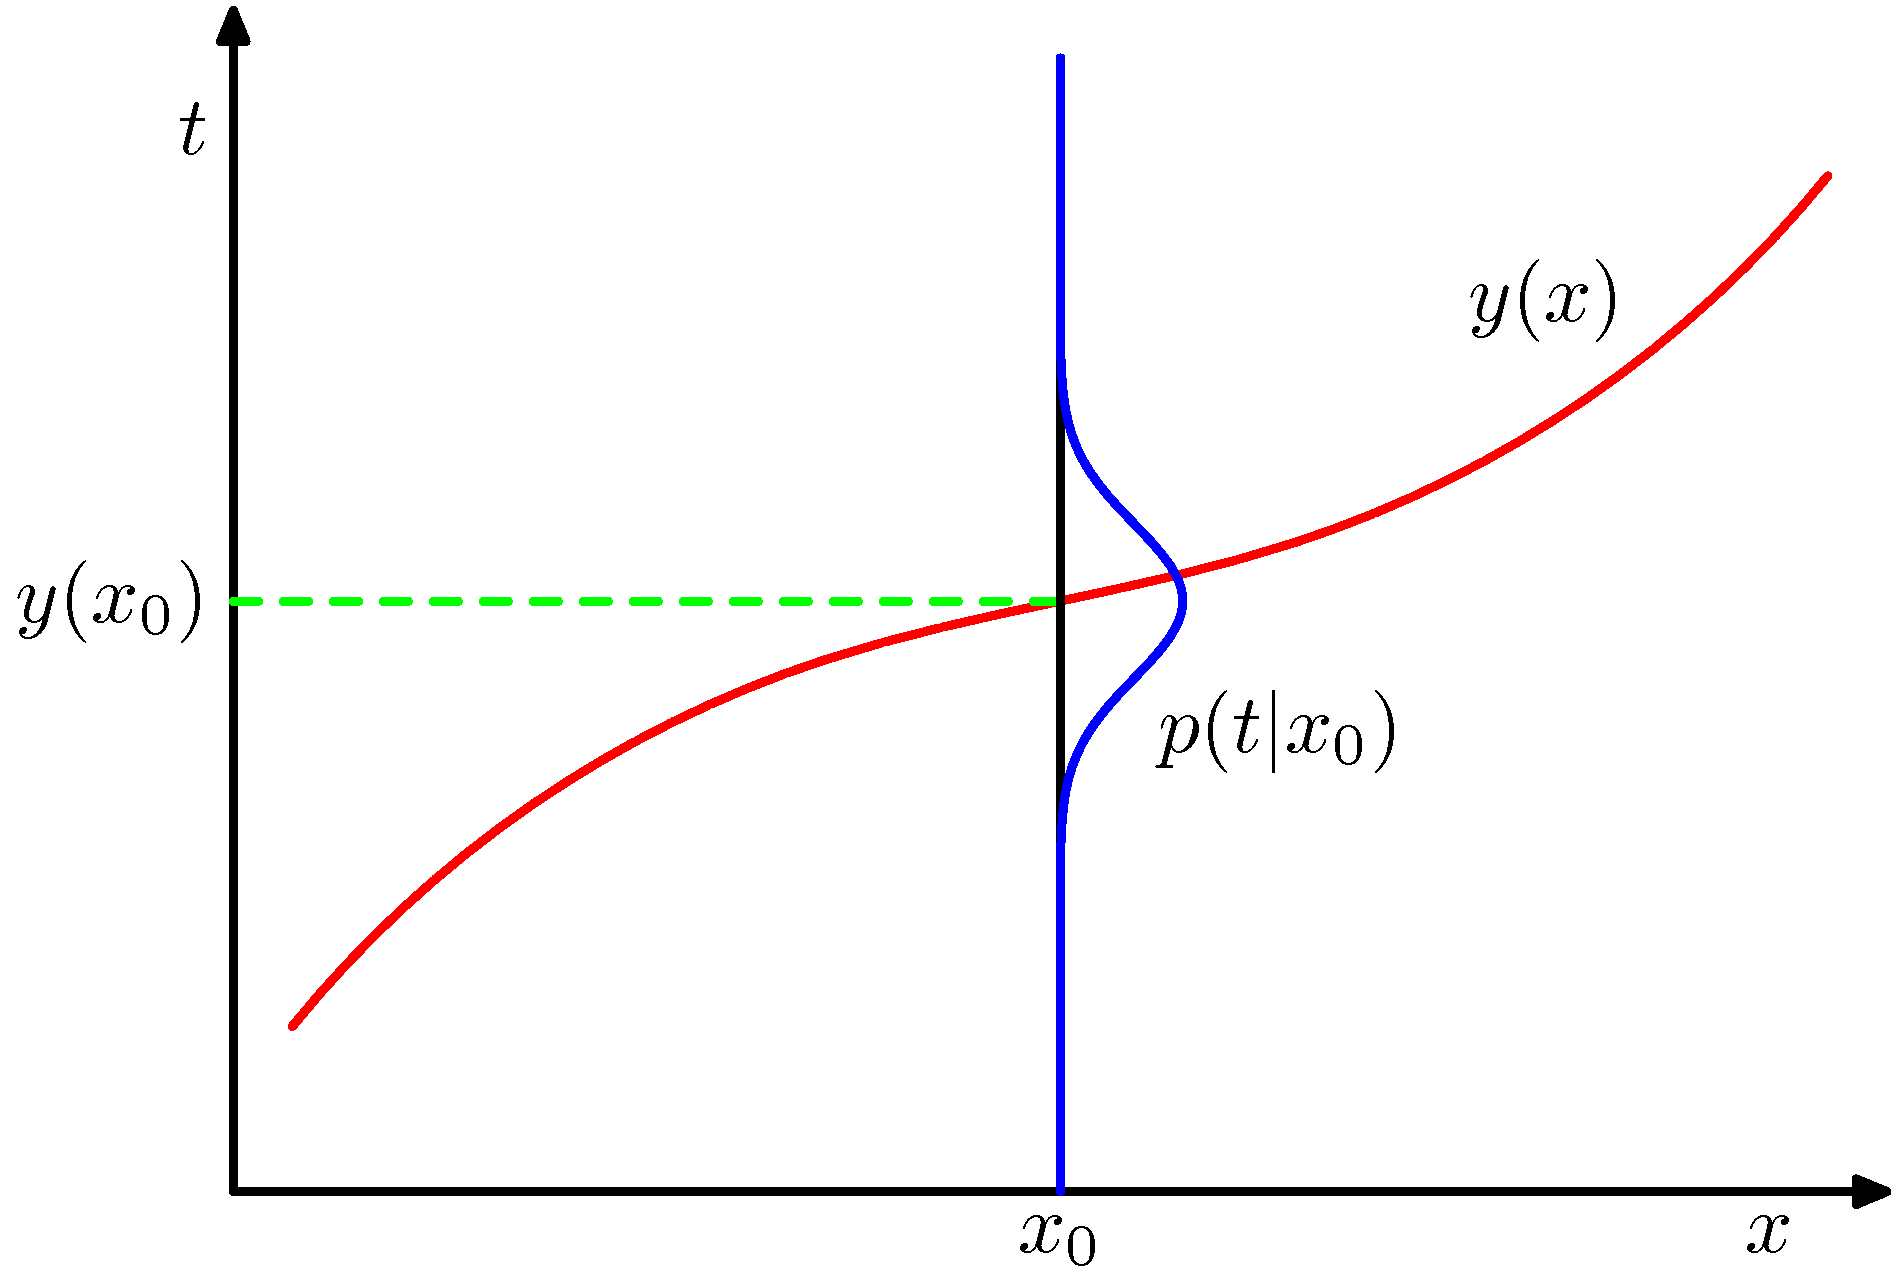
\includegraphics[scale=0.8]{Images/1-28.png}
		\captionsetup{font={small}}
		\caption{使期望平方损失最小化的回归函数y(x),由条件分布$p(t|x)$的均值得到。}
		\label{fig:1-28}
	\end{figure}
	\\
	\indent 我们同样可以利用另一种稍微不太一样的方法推出这个结论,在这个方法中将透露出回归问题的本质。我们已经知道最优解其实就是条件期望,那就可以写出平方项的展开形式:
	\[ \{y(\boldsymbol{\mathrm{x}})-t\}^2 = \{y(\boldsymbol{\mathrm{x}})-\mathbb{E}[t|\boldsymbol{\mathrm{x}}]-t\}^2 = \{y(\boldsymbol{\mathrm{x}})-\mathbb{E}[t|\boldsymbol{\mathrm{x}}]\}^2 + 2\{y(\boldsymbol{\mathrm{x}})-\mathbb{E}[t|\boldsymbol{\mathrm{x}}]\}\{\mathbb{E}[t|\boldsymbol{\mathrm{x}}]-t\}+\{\mathbb{E}[t|\boldsymbol{\mathrm{x}}]-t\}^2 \] 
	其中为了让符号简洁一些,我们用$\mathbb{E}[t|\boldsymbol{\mathrm{x}}]$来表示$\mathbb{E}_t[t|\boldsymbol{\mathrm{x}}]$。将其代入损失函数并对$t$积分,交叉项就消失了,于是就得到如下的损失函数:
	\begin{equation}
		\mathbb{E}[L]=\int \{y(\boldsymbol{\mathrm{x}})-\mathbb{E}[t|\boldsymbol{\mathrm{x}}]\}^2p(\boldsymbol{\mathrm{x}})\ \mathrm{d}\boldsymbol{\mathrm{x}} + \int \mathrm{var}[t|\bx]p(\boldsymbol{\mathrm{x}})\ \mathrm{d}\boldsymbol{\mathrm{x}}
	\end{equation}
	我们希望求取的函数$y(\boldsymbol{\mathrm{x}})$只出现在第一项中,当$y(\boldsymbol{\mathrm{x}})$等于$\mathbb{E}[t|\boldsymbol{\mathrm{x}}]$时将取得最小值,因为这时该项就会消失了。这其实就是我们刚刚证明的那个结果,最优的最小二乘预测就是条件均值。第二项是$t$的分布的方差关于$\boldsymbol{\mathrm{x}}$的平均值。它表示的是目标数据的内部变化,可以当成是噪声来处理。由于它与$y(\boldsymbol{\mathrm{x}})$相互独立,所以表示的是损失函数中不可减小的部分。\\
	\indent 与分类问题类似,我们可以通过确定适当的概率来做最优决策,也可以直接建立决策模型。同样地,我们可以明确地辨认这三种方法。根据复杂程度降序排列,这些方法分别是:\\
	\textbf{(a)}\ 首先确定联合概率密度$p(\boldsymbol{\mathrm{x}},t)$来解决推断问题。然后进行归一化来求取条件概率密度$p(t|\boldsymbol{\mathrm{x}})$,最后用(1.89)来求取条件均值。\\
	\textbf{(b)}\ 首先确定联合概率密度$p(\boldsymbol{\mathrm{x}},t)$来解决推断问题,然后用(1.89)进行边缘化来求取条件均值。\\
	\textbf{(c)}\ 直接根据训练数据求取回归函数$y(\boldsymbol{\mathrm{x}})$。\\
	\indent 这三种方法各自的优势与此前分类问题中的情况类似。\\
	\indent 平方损失并非回归问题中损失函数的唯一选择。实际上,在某些问题中利用平方损失的话可能会导致不怎么好的结果,这就需要采取更复杂一些的方法了。一个比较典型的例子就是在很多反演问题中经常出现条件分布$p(t|\boldsymbol{\mathrm{x}})$具有多个峰值(multimodal)的情况。\color{red} \textbf{——第5.6节} \color{black}在这种情况下我们就会考虑使用一种平方损失的扩展形式,叫做Minkowski损失:
	\begin{equation}
		\mathbb{E}[L_q]=\iint |y(\boldsymbol{\mathrm{x}})-t|^q p(\boldsymbol{\mathrm{x}},t)\ \mathrm{d}\boldsymbol{\mathrm{x}}\ \mathrm{d}t
	\end{equation}
	其中如果$q=2$的话就会退化为期望的平方损失。如图1.29所示是函数$|y-t|^q$关于$y-t$的图像。$\mathbb{E}[L_q]$在$q=2$时的最小值为条件均值,在$q=1$时为条件中位数,在$q \rightarrow 0$时为条件模。\color{red} \textbf{——习题 1.27} \color{black}
	\begin{figure}[ht]
		\begin{minipage}[t]{0.5\linewidth}
		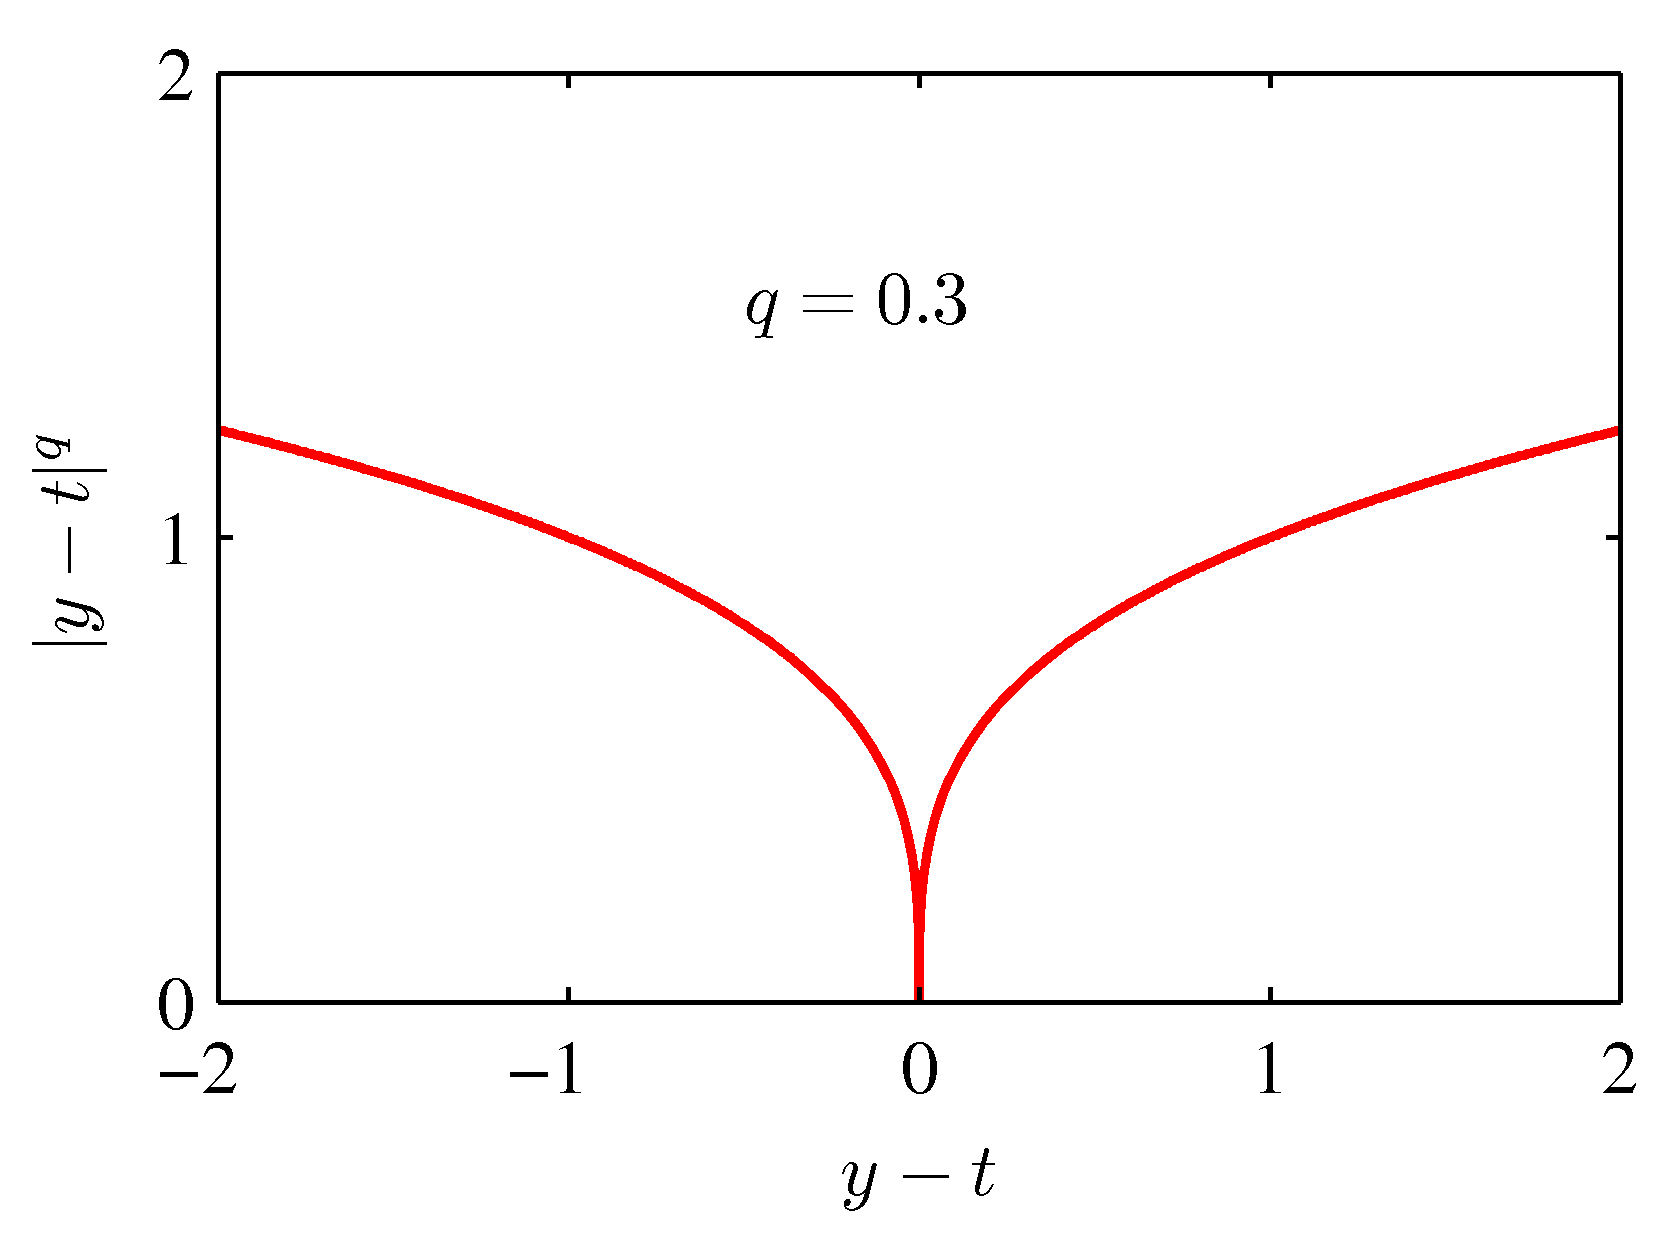
\includegraphics[scale=0.8]{Images/1-29a.png}
		\label{fig:1-29a}
		\end{minipage}
		\begin{minipage}[t]{0.5\linewidth}
		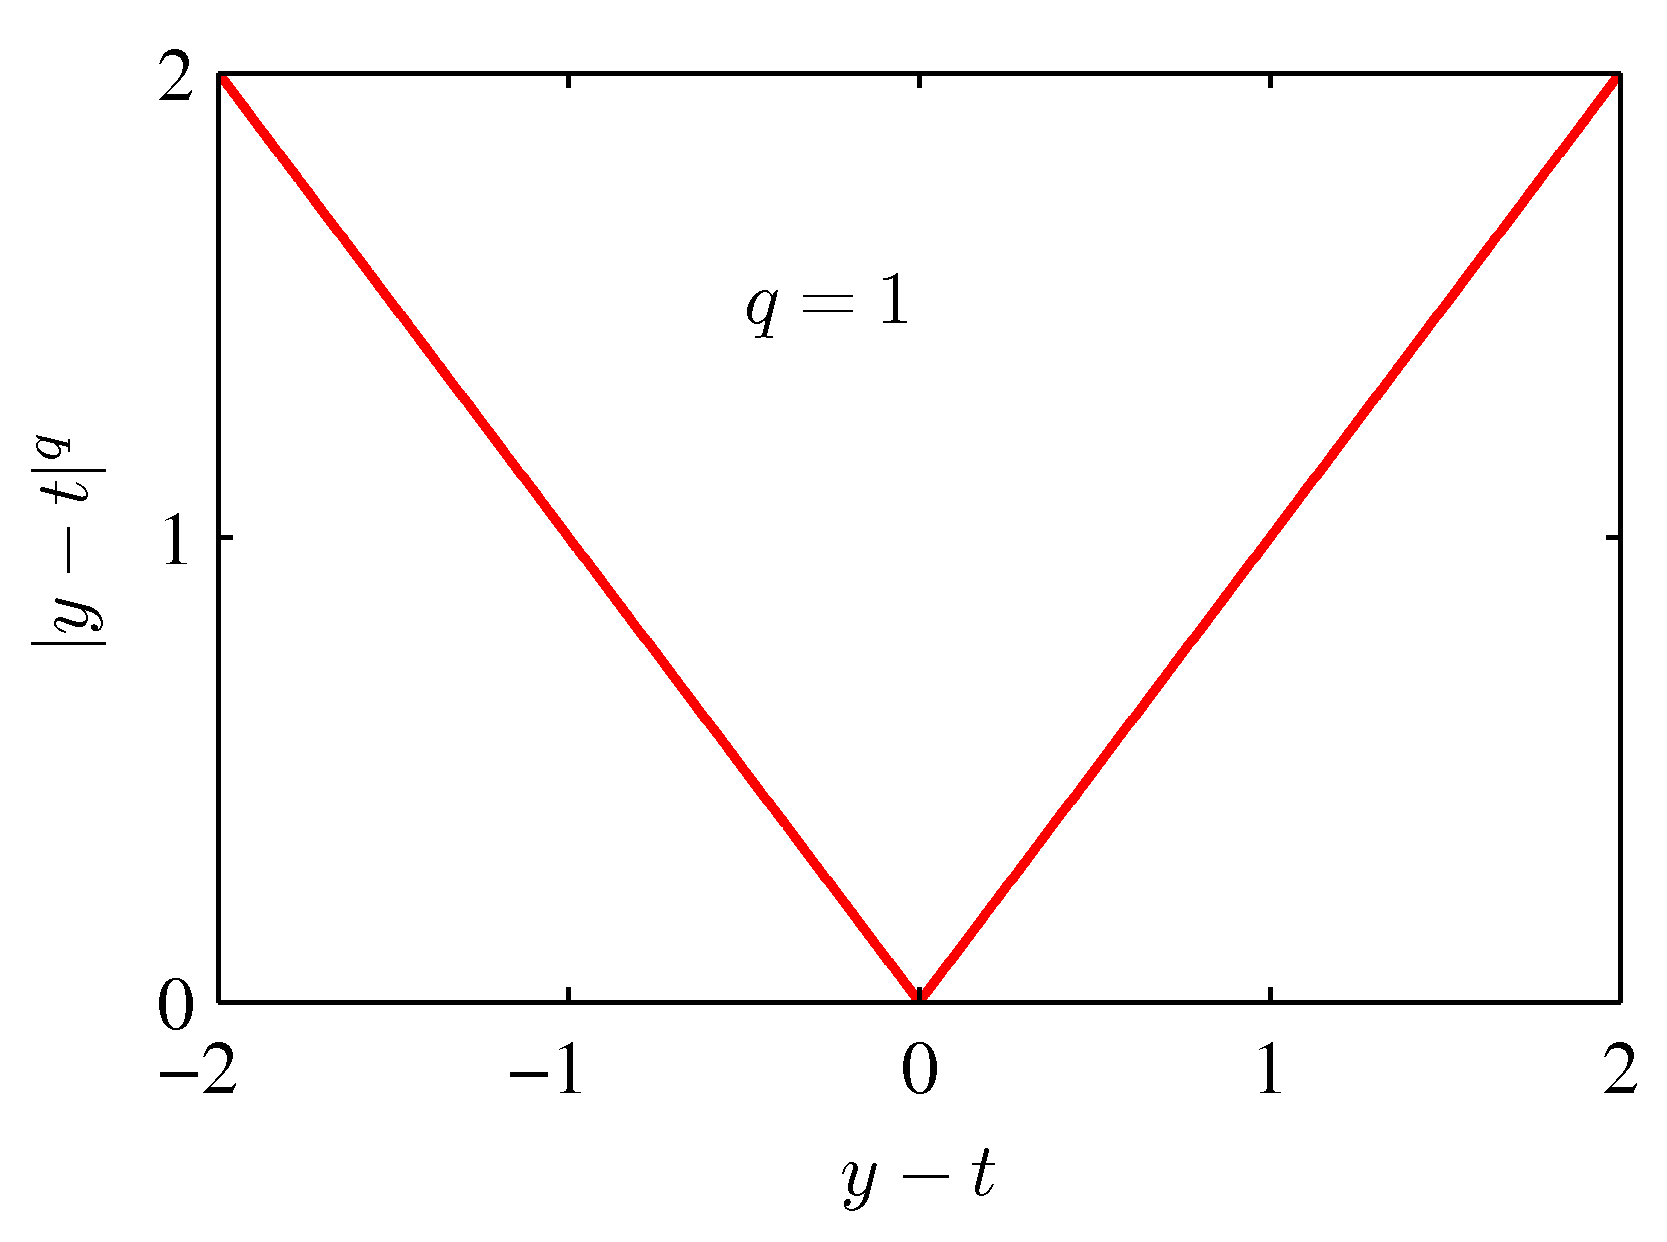
\includegraphics[scale=0.8]{Images/1-29b.png}
		\label{fig:1-29b}\\
		\end{minipage}
		\begin{minipage}[t]{0.5\linewidth}
		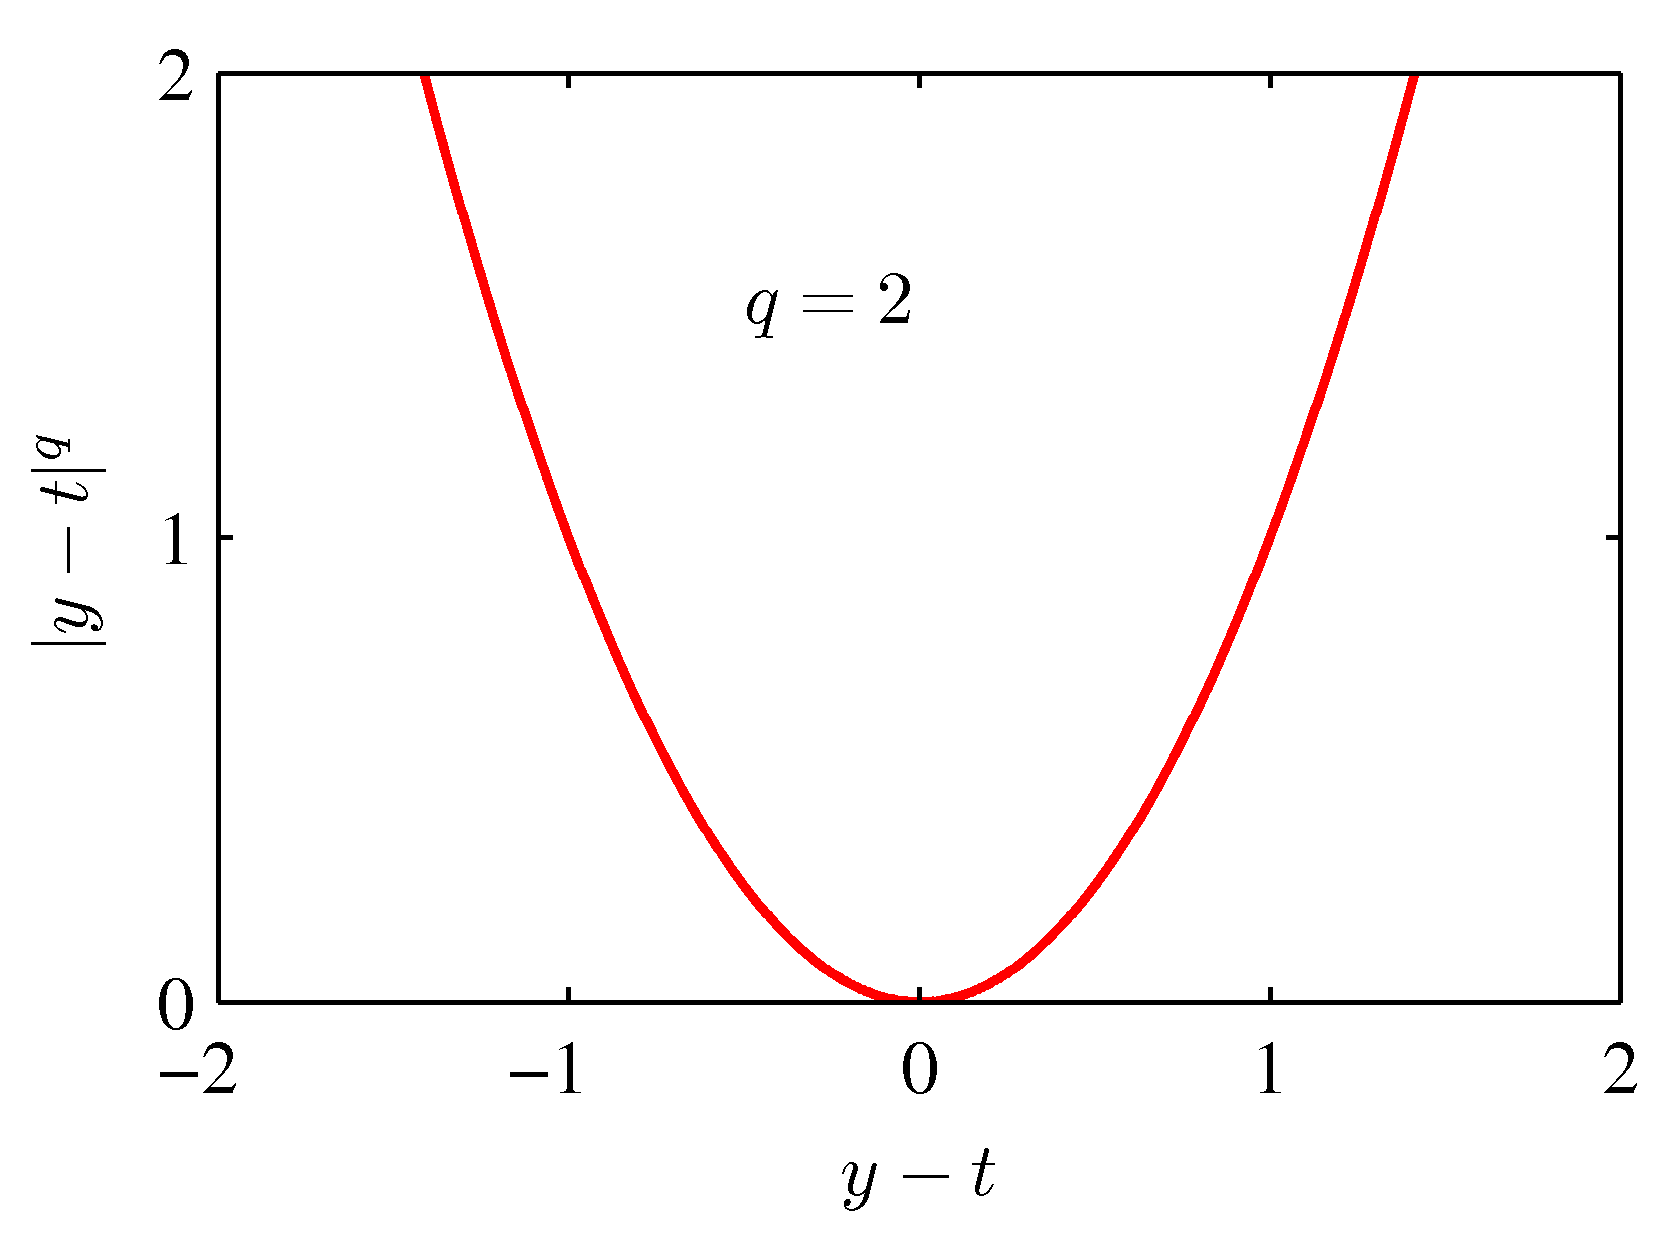
\includegraphics[scale=0.8]{Images/1-29c.png}
		\label{fig:1-29c}
		\end{minipage}
		\begin{minipage}[t]{0.5\linewidth}
		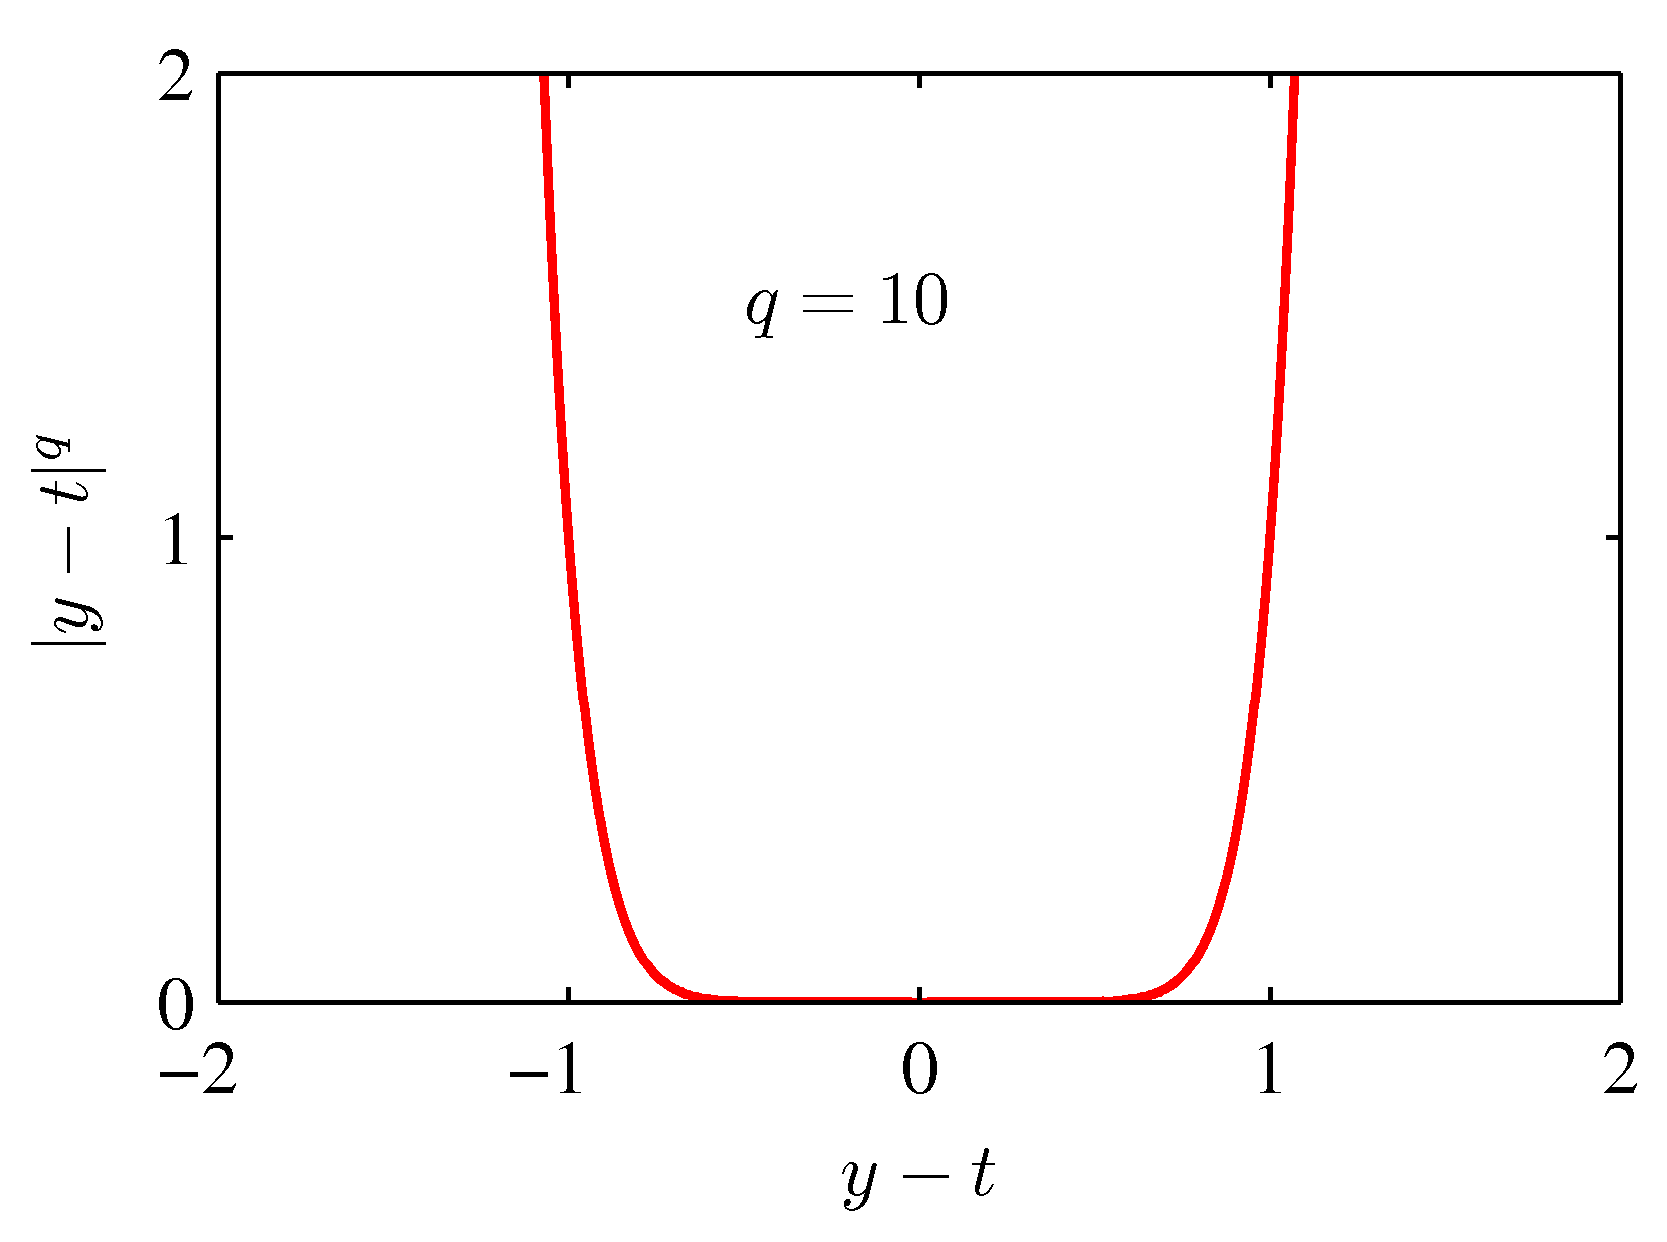
\includegraphics[scale=0.8]{Images/1-29d.png}
		\label{fig:1-29d}
		\end{minipage}
		\captionsetup{font={small}}
		\caption{函数$L_q=|y-t|^q$在$q$取不同值时的图像。}
	\end{figure}
	}
	\section{信息论}
	\noindent{\color{red} \rule[5pt]{\textwidth}{0.1em}}
	\textnormal{
	\indent 在本章中,我们已经讨论了一些概率论和决策论中的概念,这将是本书很多后续内容的基础。我们以信息论领域中一些概念的介绍来结束这个章节,这些概念同样是对模式识别与机器学习技术相当重要的。和前面一样,这里也仅仅介绍一些关键的概念,对于想要获取更多内容的读者,我们建议参考其他的文献(Viterbi and Omura, 1979; Cover and Thomas, 1991; MacKay, 2003)。\\
	\indent 我们从离散随机变量$x$开始,当我们拿到这个变量的某个值后,我们究竟获取到了多少的信息呢?信息的数量可以看成是学习$x$过程中的“惊喜程度”。比方说,要是我们刚听说有人搞了个大新闻,比起小新闻来说,我们在前者中得到的信息量肯定是更大的,要是发生的事情是日常事件,那就得不到什么信息了。对于信息量的衡量是基于概率分布$p(x)$的,于是我们就很想找到一个$p(x)$的单调函数$h(x)$,从而描述信息量。对于两个无关的事件$x$和$y$而言,$h(\cdot)$的形式比较容易确定,因为从这两个事件中得到的信息收益是从二者中分别得到的信息收益的总和,也就是$h(x,y)=h(x)+h(y)$。两个无关的事件一定是统计独立的,于是$p(x,y)=p(x)p(y)$。从这两个关系中,可以比较容易地推出,$h(x)$一定是$p(x)$的对数函数。于是可以得到\color{red} \textbf{——习题 1.28} \color{black}
	\begin{equation}
		h(x)=-\log_2p(x)
	\end{equation}
	其中的负号表示信息量是非负数。需要注意的是,一个低概率的事件$x$对应的是一个很高的信息量。对数的底数是可以随意确定的,现在我们先用信息论中比较普遍使用的以2为底数的对数。我们将会看到,在这种情况下,$h(x)$的单位是位(bits, binary digits)。\\
	\indent 现在我们假设一个信息的发送者要将某个随机变量的值传递给接收者。在传递的过程中,信息量的平均数是对(1.92)求取关于概率分布$p(x)$的期望,也就是
	\begin{equation}
		\mathrm{H}[x]=-\sum_x p(x)\log_2 p(x)
	\end{equation}
	这是一个很重要的值,称为随机变量$x$的熵(entropy)。注意,$\lim_{p \rightarrow 0} p\log_2 p = 0$,所以对于一切使得$p(x)=0$的$x$,我们认为$p(x)\log_2 p(x)=0$。\\
	\indent 到目前为止,我们用比较启发式的方式给出了信息的定义(1.92)和对应的熵的定义(1.93)。现在我们来证明这些定义确实具备实用的属性。假设一个随机变量有8个状态,每一种状态都是等可能的。为了与接收者进行$x$的交流,我们需要传递一个长度为3位的信息。注意,该变量的熵为
		\[ \mathrm{H}[x]=-8 \times \frac{1}{8}\log_2 \frac{1}{8} =3 \ \mathrm{bits} \]
	现在引入一个案例,在这个案例中8个状态$\{a,b,c,d,e,f,g,h\}$分别对应的概率是$(\frac{1}{2},\frac{1}{4},\frac{1}{8},\frac{1}{16},\frac{1}{64},\frac{1}{64},\frac{1}{64},\frac{1}{64})$。这种情况下的熵就变成了:
		\[ \mathrm{H}[x]=-\frac{1}{2}\log_2 \frac{1}{2} - \frac{1}{4}\log_2 \frac{1}{4} - \frac{1}{8}\log_2 \frac{1}{8} - \frac{1}{16}\log_2 \frac{1}{16} -\frac{4}{64}\log_2 \frac{1}{64} = 2\ \mathrm{bits} \]
	可以看出,非均匀分布的熵比均匀分布要小,从混乱程度的角度来解释熵可以让我们对此理解得更加清楚。首先我们来看究竟如何表示变量的状态取值并进行传递。和之前一样,我们可以用一个长度为3位的数字代码来表示。然而由于现在是非均匀分布,我们就可以利用这一特点让总体的代码长度短一些,用较短的代码表示概率较高的事件,但低概率事件的代码会长一些。比如说我们可以用如下代码串表示状态$\{a,b,c,d,e,f,g,h\}$:$0,10,110,1110,111100,111101,111110,111111$。需要传输的代码长度均值为:
	\[ \mathrm{average\ code\ length} = \frac{1}{2} \times 1 + \frac{1}{4} \times 2 + \frac{1}{8} \times 3 + \frac{1}{16} \times 4 + 4 \times \frac{1}{64} \times 6 = 2\ \mathrm{bits}\]
	这和随机变量的熵是相同的。但是这样的短码是不能直接拿来用的,因为可能会导致歧义,比如说,11001110这个代码串,可以解码成$c$,$a$和$d$的组合。\\
	\indent 熵与最短代码长度的关系是有关联的。无噪声编码理论(noiseless coding theorem, Shannon, 1948)表明了熵是随机变量的传递中所需要数字位数的下界。\\
	\indent 从现在开始,我们转向使用自然对数来定义熵,因为这个会为后续的内容提供不少的方便。在这种情况下,熵的单位就变成了“nats”而不是“bits”了,它们的区别仅仅在于参数$\ln 2$而已。\\
	\indent 我们已经以平均信息量的形式定义了熵,这里是需要明确随机变量的不同状态的。其实在物理学中,熵的概念要算得上长者了,它是基于平衡热力学的背景而提出,后来又在统计力学的发展中对混乱程度的衡量给出了更加深刻的解释。我们可以通过一个例子来理解熵在这个角度上的理解。假设有一组完全相同的$N$个物体,这$N$个物体会被划分到一堆箱子里,使得第$i$个箱子里有$n_i$个物体。把物体分配到箱子里的办法有多少种呢?第一个物体有$N$种选择,第二个物体有$(N-1)$种,以此类推,那么将$N$个物体分配到箱子里的办法一共有$N!$种,其中$N!$为阶乘,即$N! = N \times (N-1) \times ... \times 2 \times 1$。然而,我们又不希望对每个箱子中物体的排列顺序加以区分。在第$i$个箱子中,有$n_i!$种排列物体的方式,所以将$N$个物体分配到箱子中的方法总数为
	\begin{equation}
		W=\frac{N!}{\prod_i n_i !}
	\end{equation}
	称为“多样性”(multiplicity)。那么熵就可以定义成带有适当系数的多样性的对数
	\begin{equation}
		\mathrm{H} = \frac{1}{N}\ln W = \frac{1}{N} \ln N! - \frac{1}{N}\sum_i \ln n_i !
	\end{equation}
	现在假设$N \rightarrow \infty$,这样$n_i/N$就趋近于1了,利用斯特林公式(Stirling’s approximation):
	\begin{equation}
		\ln N! \approx N \ln N - N
	\end{equation}
	从而有
	\begin{equation}
		\mathrm{H} = - \lim_{N \rightarrow \infty} \sum_i \left( \frac{n_i}{N} \right) \ln \left( \frac{n_i}{N}\right) = -\sum_i p_i \ln p_i
	\end{equation}
	里面用到了$\sum_i n_i = N$。其中$p_i = \lim_{N \rightarrow \infty} (n_i/N)$是一个物体被分配到第$i$个箱子的概率。在物理学术语中,箱子里的物体具体排列顺序称为微观状态(microstate),而比例$n_i/N$的整体分布称为宏观状态(macrostate)。多样性$W$其实是宏观状态中的权重(weight)。\\
	\indent 我们可以将箱子解释为离散随机变量$X$的状态$x_i$,$p(X=x_i)=p_i$。那么随机变量$X$的熵就是
	\begin{equation}
		\mathrm{H}[p] = - \sum_i p(x_i)\ln p(x_i)
	\end{equation}
	在某些值附近急剧上升的分布$p(x_i)$对应的熵会比较低,而对于大多数值都比较均匀的分布的熵就相对比较高了,如图1.30所示。
	\begin{figure}[ht]
		\begin{minipage}[t]{0.5\linewidth}
		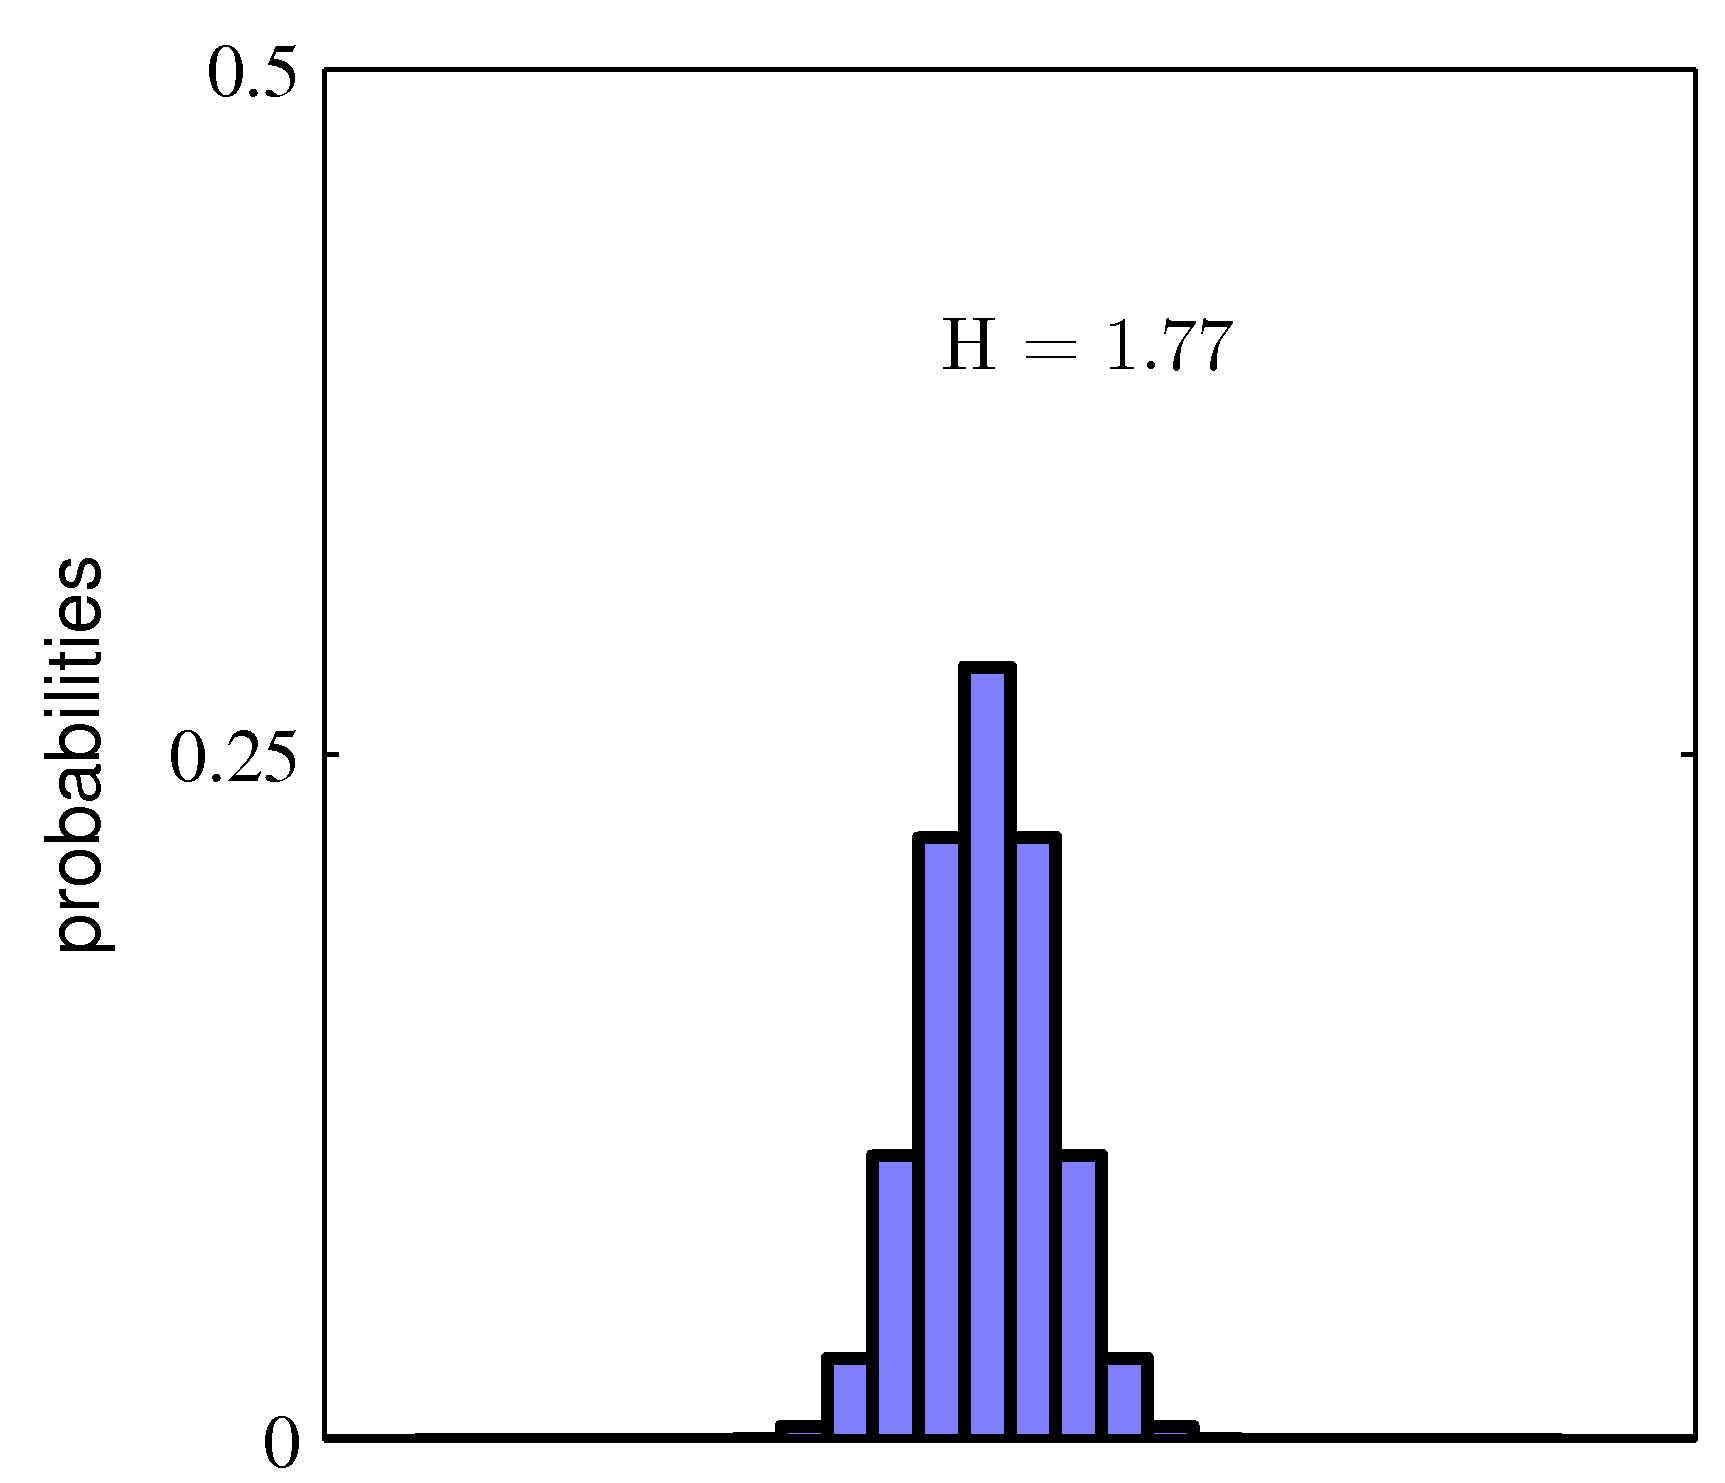
\includegraphics[scale=0.8]{Images/1-30a.png}
		\label{fig:1-30a}
		\end{minipage}
		\begin{minipage}[t]{0.5\linewidth}
		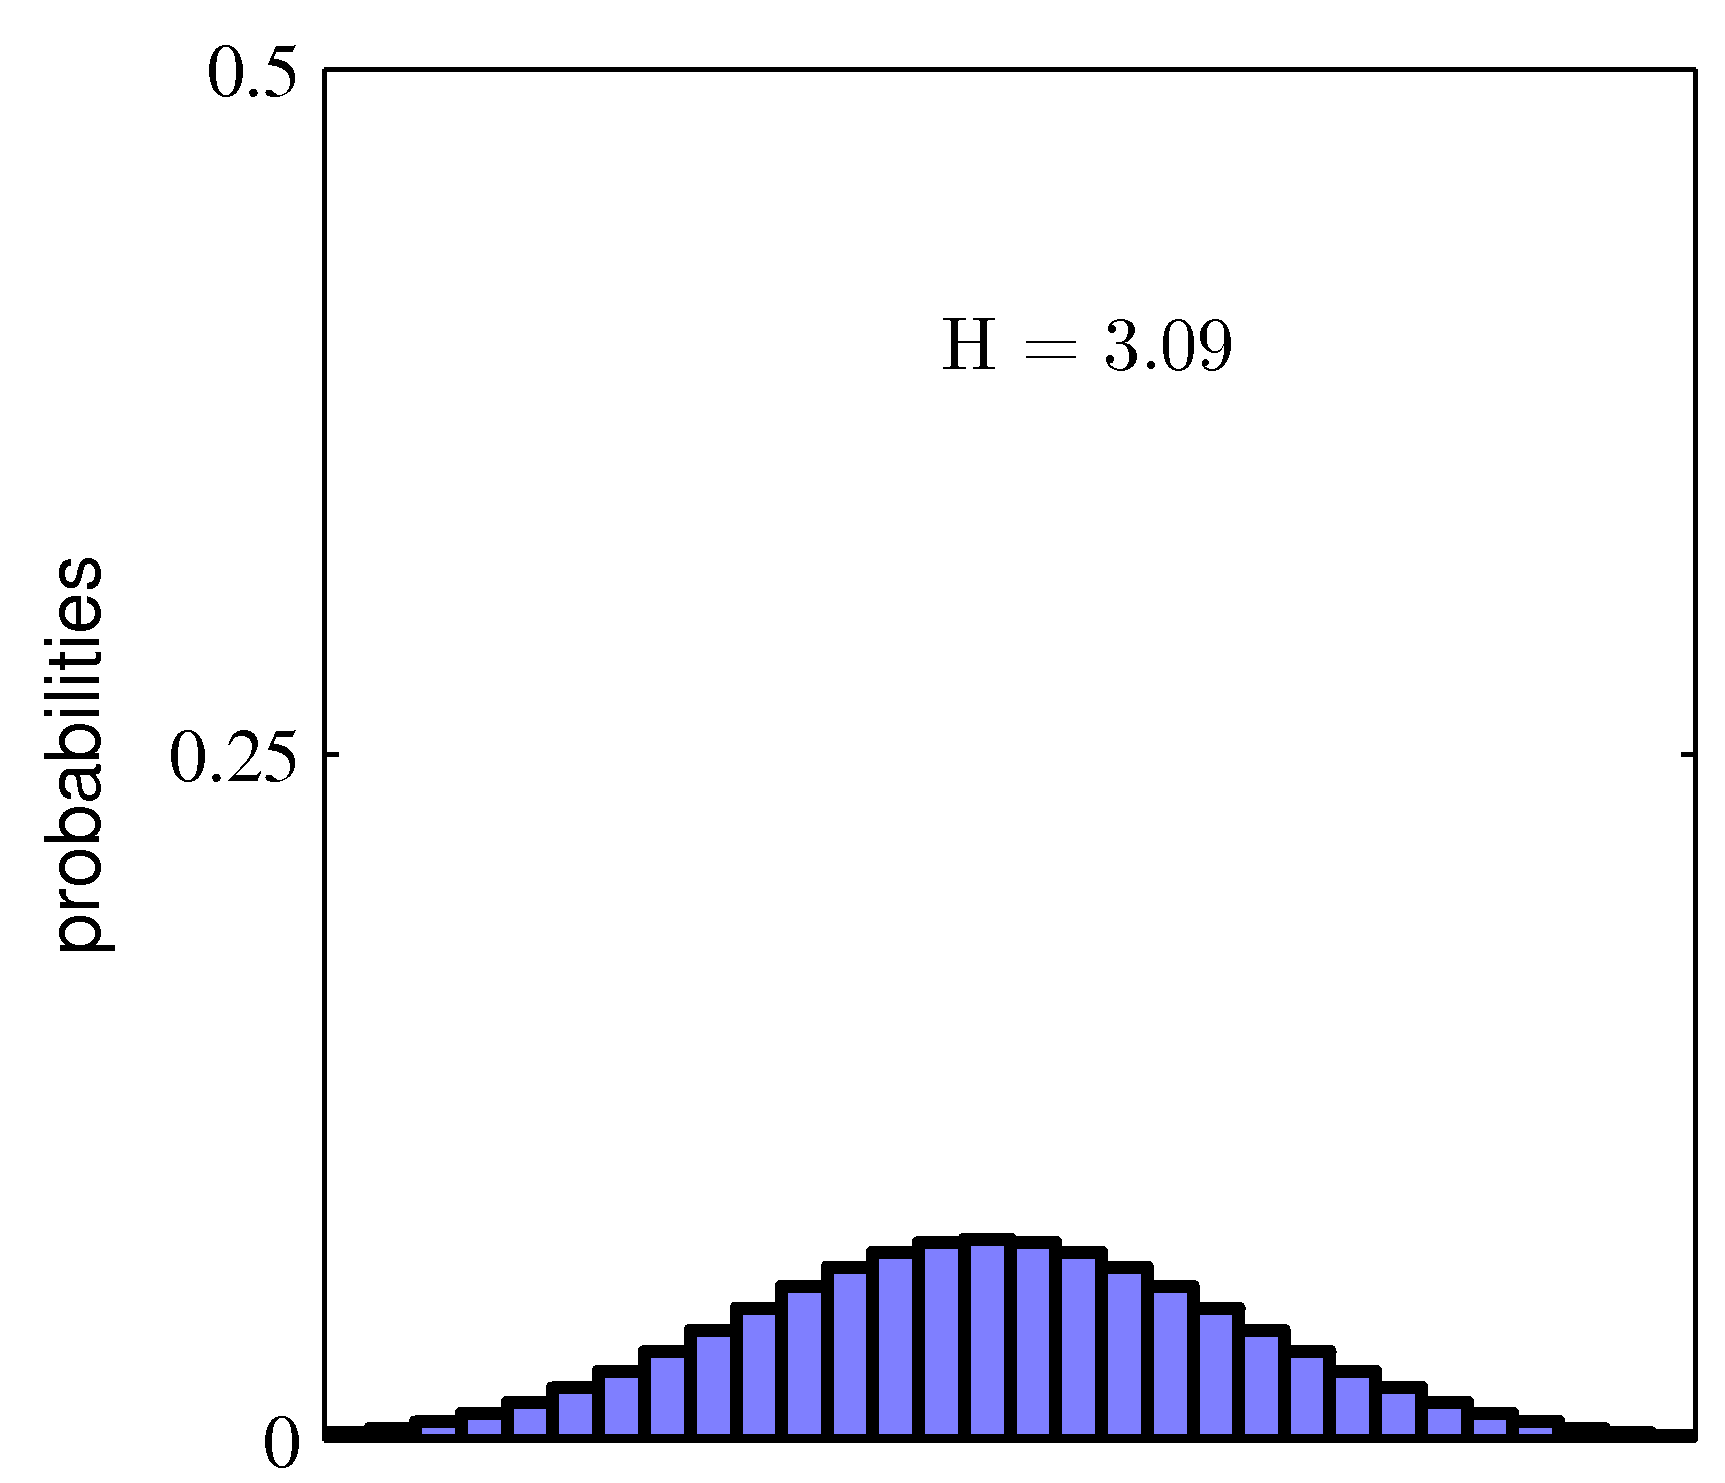
\includegraphics[scale=0.8]{Images/1-30b.png}
		\label{fig:1-30b}
		\end{minipage}
		\captionsetup{font={small}}
		\caption{以30个箱子为例,两个不同概率分布的直方图。表现越平均的分布,熵就越低。在分布为均匀分布时,熵取得最大值$\mathrm{H}=-\ln (1/30) =3.40$。}
	\end{figure}
	\\
	\indent 由于$0 \leqslant p_i \leqslant 1$,所以熵是非负数,而且当且仅当$p_i=0$且一切$p_{j \neq i} =0$时取得最小值0。另一方面可以利用拉格朗日算子进行概率归一化约束,从而对$\mathrm{H}$进行最大化来得到熵的最大值。\color{red} \textbf{——附录E} \color{black}也就是将以下函数:
	\begin{equation}
		\widetilde{\mathrm{H}} = -\sum_i p(x_i) \ln p(x_i) + \lambda \left(\sum_i p(x_i)-1 \right)
	\end{equation}
	进行最大化。我们会发现,在取得最大值时所有的$p(x_i)$都是相等的,而且$p(x_i)=1/M$,$M$为状态$x_i$的总数。对应的熵就是$\mathrm{H} = \ln M$。这个结果也可以通过Jensen不等式来推导出来。\color{red} \textbf{——习题 1.29} \color{black}为了确定驻点处确实是最大值,可以对熵求二阶导数,也就是
	\begin{equation}
		\frac{\partial\mathrm{^2} \widetilde{H}}{\partial p(x_i) \partial p(x_j)} = -I_{ij}\frac{1}{p_i}
	\end{equation}
	其中$I_{ij}$为单位矩阵的元素。\\
	\indent 我们可以将熵的定义扩展为到连续变量$x$的分布上。首先将$x$分配到宽度为$\Delta$的区间中;然后假设$p(x)$是连续的,根据中值定理(mean value theorem, Weisstein, 1999),对于任意区间,一定存在$x_i$,使得
	\begin{equation}
		\int_{i\Delta}^{(i+1)\Delta} p(x)\ \mathrm{d}x = p(x_i) \Delta
	\end{equation}
	现在我们可以通过在$x$落入第$i$个区间时给$x$任意赋值来量化连续变量$x$了。那么观测到$x_i$值的概率就是$p(x_i)\Delta$。这就给出了一个离散形式的计算熵的方式:
	\begin{equation}
		\mathrm{H}_{\Delta}=-\sum_{i}p(x_i)\Delta \ln(p(x_i)\Delta) = -\sum_i p(x_i)\Delta \ln p(x_i)-\ln \Delta
	\end{equation}
	与(1.101)一样,其中$\sum_i p(x_i) \Delta =1$。现在我们直接忽略(1.102)等号右侧的第二项$\ln \Delta$,并取极限$\Delta \rightarrow 0$。(1.102)等号右侧的第一项在取极限时会趋近于$p(x)\ln p(x)$的积分,也就是
	\begin{equation}
		\lim_{\Delta \rightarrow 0} \left\{ - \sum_i p(x_i)\Delta \ln p(x_i) \right\} = -\int p(x)\ln p(x)\ \mathrm{d}x
	\end{equation}
	其中等号右侧的值称为差分熵(differential entropy)。我们可以看出,熵的离散形式和连续形式的区别在于$\ln \Delta$,在$\Delta \rightarrow 0$时会发散。这反映了想要非常精确地直接指定一个连续变量,需要很多位才行。对于多个连续变量的概率密度,用$\boldsymbol{\mathrm{x}}$表示变量组成的向量,则差分熵为
	\begin{equation}
		\mathrm{H}[\boldsymbol{\mathrm{x}}] = -\int p(\boldsymbol{\mathrm{x}}) \ln p(\boldsymbol{\mathrm{x}}) \mathrm{d}\boldsymbol{\mathrm{x}}
	\end{equation}
	\indent 在离散分布中,我们发现最大熵是在变量的分布为均匀分布时取得的。现在我们考虑一下连续分布的情况。为了确定这个情况下熵的最大值,引入对$p(x)$的一阶矩、二阶矩的约束,以及归一化约束是很有必要的。这三个约束分别是
	\begin{align}
		\int_{-\infty}^{\infty} p(x)\ \mathrm{d}x &= 1 \\
		\int_{-\infty}^{\infty} xp(x)\ \mathrm{d}x &= \mu \\
		\int_{-\infty}^{\infty} (x-\mu)^2p(x)\ \mathrm{d}x &= \sigma^2
	\end{align}
	这个约束优化问题可以利用拉格朗日算子来解决。\color{red} \textbf{——附录 E} \color{black}于是我们关于$p(x)$对以下式子求最大值:
	\begin{equation*}
	\begin{split}
		&-\int_{-\infty}^{\infty} p(x)\ln p(x)\ \mathrm{d}x + \lambda_1 \left(\int_{-\infty}^{\infty} p(x)\ \mathrm{d}x -1\right)\\
		&+ \lambda_2 \left(\int_{-\infty}^{\infty} xp(x)\ \mathrm{d}x -\mu \right) +\lambda_3\left(\int_{-\infty}^{\infty} (x-\mu)^2p(x)\ \mathrm{d}x - \sigma^2\right)
	\end{split}
	\end{equation*}
	采用变分法(\color{red} \textbf{附录 D}\color{black}),设该式的导数为0,于是
	\begin{equation}
		p(x)=\exp\left\{-1+\lambda_1+\lambda_2 x + \lambda_3(x-\mu)^2\right\}
	\end{equation}
	拉格朗日算子可以通过将这个结果回代到此前的三个约束等式中,最终的结果为\color{red} \textbf{——习题 1.34} \color{black}
	\begin{equation}
		p(x)=\frac{1}{(2\pi\sigma^2)^{1/2}}\exp\left\{-\frac{(x-\mu)^2}{2\sigma^2}\right\}
	\end{equation}
	所以使得差分熵取得最大值的分布就是高斯分布。需要注意的是,我们没有基于熵必须不小于0来建立约束。然而,最后我们得到的分布确实是非负的,可以看出这个约束是没有必要的。\\
	\indent 如果我们对高斯分布求取差分熵,可以得到\color{red} \textbf{——习题 1.35} \color{black}
	\begin{equation}
		\mathrm{H}[x]=\frac{1}{2}\left\{1+\ln(2\pi\sigma^2)\right\}
	\end{equation}
	于是我们可以再次看出,$\sigma^2$越大,分布就越“宽”,熵就越大。这个结果显示,与离散熵不同,差分熵是可能取负数的,因为(1.110)中的$\mathrm{H}(x)$在$\sigma^2<1/(2\pi e)$时小于0。\\
	\indent 假设我们有一个联合概率分布$p(\boldsymbol{\mathrm{x}},\boldsymbol{\mathrm{y}})$,其中$\boldsymbol{\mathrm{x}}$和$\boldsymbol{\mathrm{y}}$是成对的。如果一个$\boldsymbol{\mathrm{x}}$已知,那么确定$\boldsymbol{\mathrm{y}}$需要的附加信息是$-\ln p(\boldsymbol{\mathrm{y}}|\boldsymbol{\mathrm{x}})$。于是确定$\boldsymbol{\mathrm{y}}$需要的平均附加信息可以写成:
	\begin{equation}
		\mathrm{H}[\boldsymbol{\mathrm{y}}|\boldsymbol{\mathrm{x}}]=-\iint p(\boldsymbol{\mathrm{y}},\boldsymbol{\mathrm{x}})\ln p(\boldsymbol{\mathrm{y}}|\boldsymbol{\mathrm{x}})\ \mathrm{d}\boldsymbol{\mathrm{y}}\ \mathrm{d}\boldsymbol{\mathrm{x}}
	\end{equation}
	上式称为给定$\boldsymbol{\mathrm{x}}$的条件下$\boldsymbol{\mathrm{y}}$的条件熵(conditional entropy)。可以比较容易地看出,利用乘法规则,条件熵满足\color{red} \textbf{——习题 1.37} \color{black}
	\begin{equation}
		\mathrm{H}[\boldsymbol{\mathrm{x}},\boldsymbol{\mathrm{y}}] = \mathrm{H}[\boldsymbol{\mathrm{y}}|\boldsymbol{\mathrm{x}}] + \mathrm{H}[\boldsymbol{\mathrm{x}}]
	\end{equation}
	其中$\mathrm{H}[\boldsymbol{\mathrm{x}},\boldsymbol{\mathrm{y}}]$为$p(\boldsymbol{\mathrm{x}},\boldsymbol{\mathrm{y}})$的差分熵,$\mathrm{H}[\boldsymbol{\mathrm{x}}]$为边缘概率分布$p(\boldsymbol{\mathrm{x}})$的差分熵。于是用于描述$\boldsymbol{\mathrm{x}}$和$\boldsymbol{\mathrm{y}}$的信息可以由描述$\boldsymbol{\mathrm{x}}$所需的信息加上给定$\boldsymbol{\mathrm{x}}$的情况下确定$\boldsymbol{\mathrm{y}}$所需的附加信息来得到。}
	\subsection{相对熵与互信息}
	\textnormal{在本节此前的内容中,我们已经介绍了信息论的一些相关概念,包括最重要的关于熵的定义和分析。现在我们开始将这些内容应用于模式识别。假设我们现在有一个未知的分布$p(\boldsymbol{\mathrm{x}})$,并利用一个近似的分布$q(\boldsymbol{\mathrm{x}})$对它进行建模。如果我们利用$q(\boldsymbol{\mathrm{x}})$来对此前提出的$\boldsymbol{\mathrm{x}}$值的传递构建编码方案,那么根据$q(\boldsymbol{\mathrm{x}})$而非真实分布$p(\boldsymbol{\mathrm{x}})$给定的$\boldsymbol{\mathrm{x}}$的值(假设我们选择了很高效的编码方案)的情况下,信息的平均附加量(以nats为单位)可以根据以下公式计算:
	\begin{equation}
		\begin{split}
			\mathrm{KL}(p||q) &= -\int p(\boldsymbol{\mathrm{x}})\ln q(\boldsymbol{\mathrm{x}}) - \left(-\int p(\boldsymbol{\mathrm{x}})\ln q(\boldsymbol{\mathrm{x}})\ \mathrm{d}\boldsymbol{\mathrm{x}}\right) \\
			&= -\int p(\boldsymbol{\mathrm{x}}) \ln \left\{\frac{q(\boldsymbol{\mathrm{x}})}{p(\boldsymbol{\mathrm{x}})}\ \mathrm{d}\boldsymbol{\mathrm{x}} \right\}
		\end{split}
	\end{equation}
	这就是分布$p(\boldsymbol{\mathrm{x}})$和$q(\boldsymbol{\mathrm{x}})$之间的相对熵(relative entropy)或者称为Kullback-Leibler距离,亦或称为KL差(Kullback and Leibler, 1951)。需要注意的是,这个公式并不具备对称性,也就是说$\mathrm{KL}(p||q) \neq \mathrm{KL}(q||p)$。\\
	\indent 现在我们来证明Kullback-Leibler距离满足$\mathrm{KL}(p||q) \geqslant 0$,当且仅当$p(\boldsymbol{\mathrm{x}})=q(\boldsymbol{\mathrm{x}})$时等号成立。为了证明这个问题,我们首先介绍凸函数(convex function)的概念。如果函数$f(x)$的任意一条弦要么位于函数上,要么位于函数的上方,那么函数$f(x)$就是凸函数,如图1.31所示。
	\begin{figure}[ht]
		\centering
		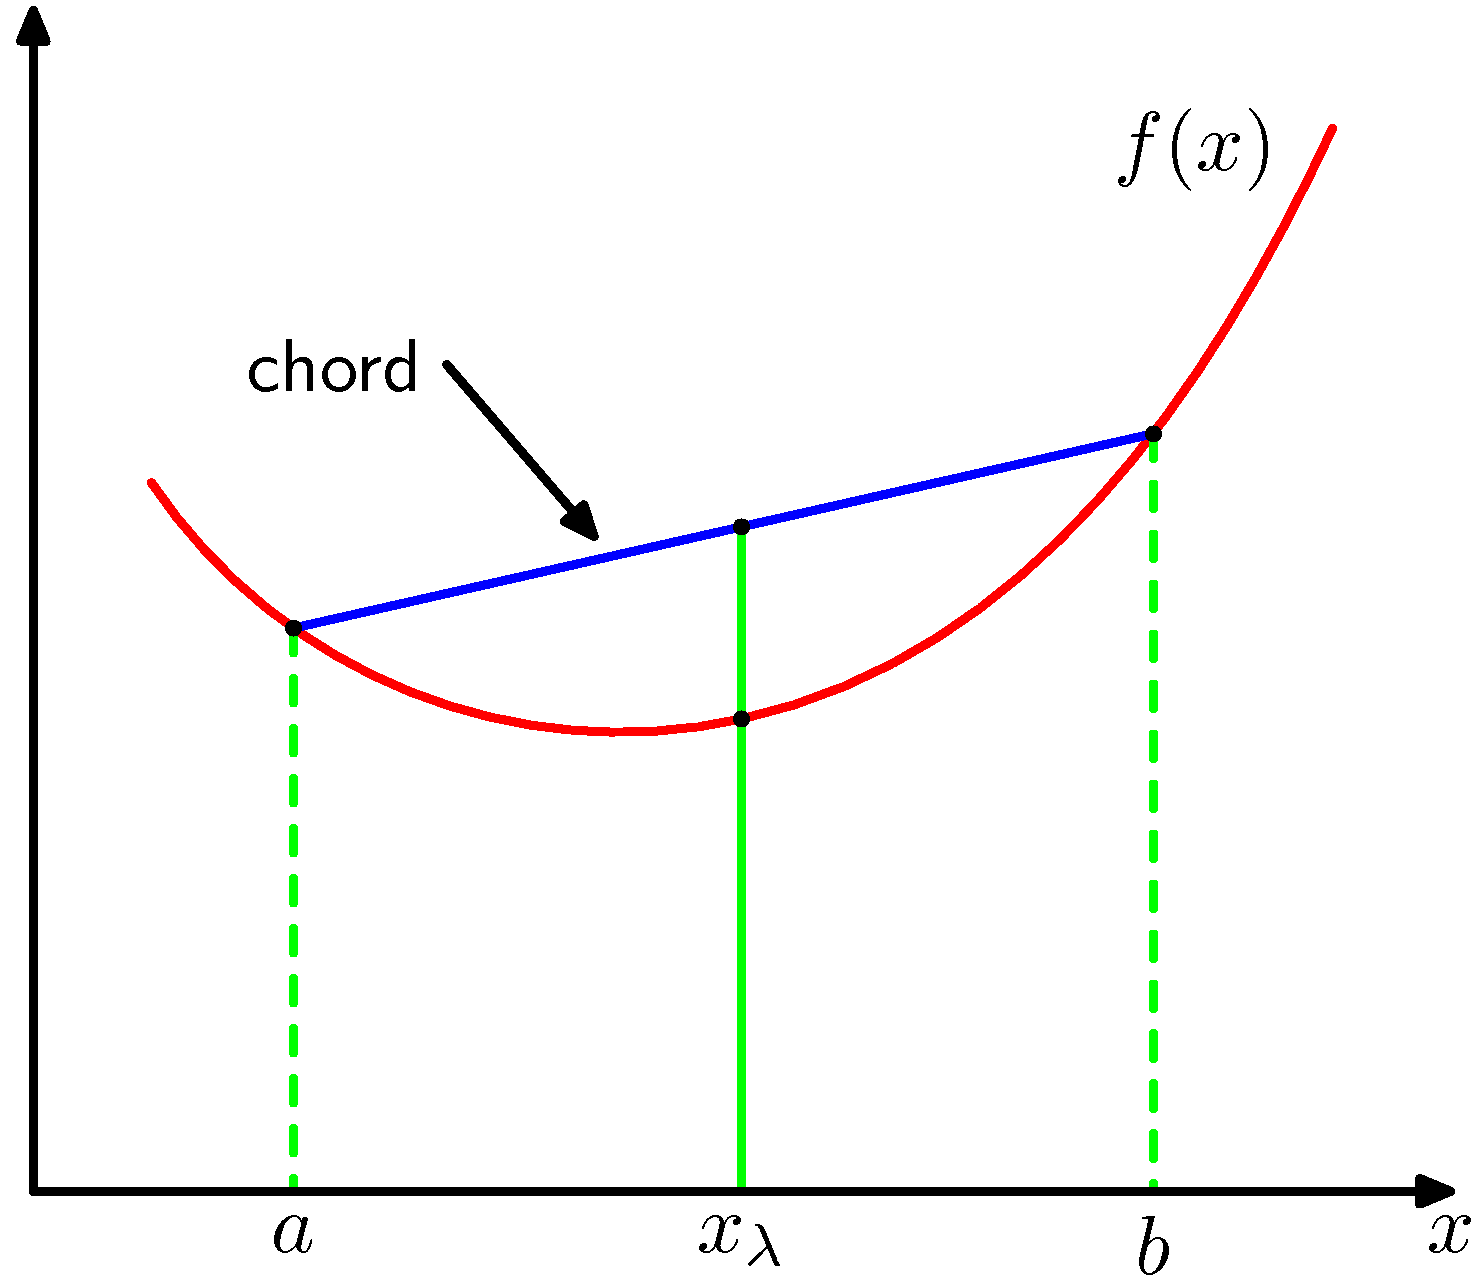
\includegraphics[scale=0.8]{Images/1-31.png}
		\captionsetup{font={small}}
		\caption{凸函数$f(x)$。它的每条弦(蓝色直线)都在自身(红色曲线)上或者自身的上方。}
		\label{fig:1-31}
	\end{figure}
	\\
	\indent 对于$x=a$和$x=b$区间内所有的$x$都可以写成$\lambda a + (1-\lambda) b$的形式,其中$0 \leqslant \lambda \leqslant 1$,在弦上对应的点是$\lambda f(a) + (1-\lambda) f(b)$,对应的函数值为$f(\lambda a + (1-\lambda)b)$。于是有一条性质:
	\begin{equation}
		f(\lambda a + (1-\lambda)b) \leqslant \lambda f(a) + (1-\lambda)f(b)
	\end{equation}
	这个性质与函数的二阶导数处处为正是等价的。\color{red} \textbf{——习题 1.36} \color{black}凸函数的典型例子是$x\ln x (x>0)$和$x^2$。如果上式中的等号仅在$\lambda=0$和$\lambda=1$时成立,那么$f(x)$就是严格凸函数(strictly convex function)。如果一个函数有与此相反的性质,也就是说每一条弦都位于函数上或函数下方,那么就称为凹函数(concave function),对应的还有严格凹函数(strictly concave function)。如果$f(x)$为凸函数,那么$-f(x)$一定为凹函数。\\
	\indent 利用归纳法,根据(1.114)可以证明凸函数$f(x)$满足:\color{red} \textbf{——习题 1.38} \color{black}
	\begin{equation}
		f\left(\sum_{i=1}^M \lambda_i x_i\right) \leqslant \sum_{i=1}^M \lambda_i f(x_i)
	\end{equation}
	\indent 对于任意的$\{x_i\}$集合,$\lambda_i \geqslant 0$ 且$\sum_i \lambda_i =1$。公式(1.115)就是Jensen不等式。如果我们将$\lambda_i$看成是取值为$\{x_i\}$的离散随机变量$x$的概率分布,那么(1.115)就可以写成
	\begin{equation}
		f(\mathbb{E}[x])\leqslant \mathbb{E}[f(x)]
	\end{equation}
	其中$\mathbb{E}(\cdot)$表示期望。对于连续变量,Jensen不等式的形式为
	\begin{equation}
		f\left(\int \boldsymbol{\mathrm{x}}p(\boldsymbol{\mathrm{x}})\ \mathrm{d}\boldsymbol{\mathrm{x}}\right) \leqslant \int f(\boldsymbol{\mathrm{x}})p(\boldsymbol{\mathrm{x}})\ \mathrm{d}\boldsymbol{\mathrm{x}}
	\end{equation}
	\indent 我们可以将(1.117)中的Jensen不等式带入到(1.113)中的Kullback-Leibler距离中,于是有
	\begin{equation}
		\mathrm{KL}(p||q) = - \int p(\boldsymbol{\mathrm{x}}) \ln \left\{\frac{q(\boldsymbol{\mathrm{x}})}{p(\boldsymbol{\mathrm{x}})}\right\}\ \mathrm{d}\boldsymbol{\mathrm{x}} \geqslant - \ln \int q(\boldsymbol{\mathrm{x}})\ \mathrm{d}\boldsymbol{\mathrm{x}} = 0
	\end{equation}
	其中用到了一些结论——$\ln x$是一个凸函数,以及归一化条件$\int q(\boldsymbol{\mathrm{x}})\ \mathrm{d}\boldsymbol{\mathrm{x}} = 1$。实际上,$-\ln x$是一个严格凸函数,所以对于一切$\boldsymbol{\mathrm{x}}$当且仅当$q(\boldsymbol{\mathrm{x}})=p(\boldsymbol{\mathrm{x}})$时等号成立。于是我们就可以将Kullback-Leibler距离看成是两个分布$p(\boldsymbol{\mathrm{x}})$和$q(\boldsymbol{\mathrm{x}})$之间的不相似程度的衡量。\\
	\indent 我们看到,数据的压缩与密度估计(即对未知概率分布进行建模的问题)之间存在密切的联系。因为当我们知道真实的分布之后,就可以对数据进行最有效的压缩。如果我们用了一个与真实分布不同的分布,那么编码一定是会变得低效一些的。而且就常规情况而言,必须要加入到传输之中的附加信息(至少)等于两个分布之间的Kullback-Leibler距离。\\
	\indent 假设数据是从我们希望建模的未知分布$p(\boldsymbol{\mathrm{x}})$生成的。我们可以利用带有可调整参数$\boldsymbol{\mathrm{\theta}}$的参数分布$q(\boldsymbol{\mathrm{x}}|\boldsymbol{\mathrm{\theta}})$来接近这个分布,比如说多元高斯分布。确定参数$\boldsymbol{\mathrm{\theta}}$的方法之一就是关于$\boldsymbol{\mathrm{\theta}}$求取$p(\boldsymbol{\mathrm{x}})$与$p(\boldsymbol{\mathrm{x}}|\boldsymbol{\mathrm{\theta}})$之间Kullback-Leibler距离的最小值。但我们不能直接用这个方法,因为$p(\boldsymbol{\mathrm{x}})$是未知的。不过,假设我们有一个从$p(\boldsymbol{\mathrm{x}})$中取出的有限训练集$\boldsymbol{\mathrm{x}}_n, n=1,...,N$,那么关于$p(\boldsymbol{\mathrm{x}})$的期望就可以用这些数据的有限和,根据(1.35)来逼近。于是
	\begin{equation}
		\mathrm{KL}(p||q)\approx \frac{1}{N}\sum_{n=1}^{N}{-\ln q(\boldsymbol{\mathrm{x}}_n|\boldsymbol{\mathrm{\theta}})+\ln p(\boldsymbol{\mathrm{x}}_n)}
	\end{equation}
	(1.119)中等号右侧的第二项是与$\boldsymbol{\mathrm{\theta}}$相互独立的,第一项是根据训练集估计得到的$\boldsymbol{\mathrm{\theta}}$的分布$q(\boldsymbol{\mathrm{x}}|\boldsymbol{\mathrm{\theta}})$的负对数似然函数。于是我们可以看出,将Kullback-Leibler距离进行最小化,等价于将似然函数进行最大化。\\
	\indent 下面考虑两个变量集合的联合分布$p(\boldsymbol{\mathrm{x}},\boldsymbol{\mathrm{y}})$。如果两个变量集合是相互独立的,那么它们的联合分布就可以拆分成各自边缘分布的乘积$p(\boldsymbol{\mathrm{x}},\boldsymbol{\mathrm{y}})=p(\boldsymbol{\mathrm{x}})p(\boldsymbol{\mathrm{y}})$。如果它们不是相互独立的,我们可以通过研究联合分布与边缘分布乘积之间的Kullback-Leibler距离来衡量这两组变量有多么“接近”相互独立,根据以下公式计算:
	\begin{equation}
		\begin{split}
			\mathrm{I}[\boldsymbol{\mathrm{x}},\boldsymbol{\mathrm{y}}] &\equiv \mathrm{KL}(p(\boldsymbol{\mathrm{x}},\boldsymbol{\mathrm{y}})p(\boldsymbol{\mathrm{x}})p(\boldsymbol{\mathrm{y}}))\\
			&=-\iint p(\boldsymbol{\mathrm{x}},\boldsymbol{\mathrm{y}}) \ln \left(\frac{p(\boldsymbol{\mathrm{x}})p(\boldsymbol{\mathrm{y}})}{p(\boldsymbol{\mathrm{x}},\boldsymbol{\mathrm{y}})}\right)\ \mathrm{d}\boldsymbol{\mathrm{x}}\ \mathrm{d}\boldsymbol{\mathrm{y}}
		\end{split}
	\end{equation}
	该结果称为变量$\boldsymbol{\mathrm{x}}$与$\boldsymbol{\mathrm{y}}$之间的互信息(nutual information)。根据Kullback-Leibler距离的性质,可以看出$\mathrm{I}(\boldsymbol{\mathrm{x}},\boldsymbol{\mathrm{y}}) \geqslant 0$,当且仅当$\boldsymbol{\mathrm{x}}$与$\boldsymbol{\mathrm{y}}$相互独立时等号成立。利用概率的加法规则和乘法规则,可以看出互信息与条件熵是相关的:\color{red} \textbf{——习题 1.41} \color{black}
	\begin{equation}
		\mathrm{I}[\boldsymbol{\mathrm{x}},\boldsymbol{\mathrm{y}}]=\mathrm{H}[\boldsymbol{\mathrm{x}}]-\mathrm{H}[\boldsymbol{\mathrm{x}}|\boldsymbol{\mathrm{y}}]=\mathrm{H}[\boldsymbol{\mathrm{y}}]-\mathrm{H}[\boldsymbol{\mathrm{y}}|\boldsymbol{\mathrm{x}}]
	\end{equation}
	于是可以将互信息看成是给出$\boldsymbol{\mathrm{y}}$的情况下减少的$\boldsymbol{\mathrm{x}}$的不确定性(反之亦然)。从贝叶斯学派的角度来看,我们可以将$p(\boldsymbol{\mathrm{x}})$看成是$\boldsymbol{\mathrm{x}}$的先验分布,$p(\boldsymbol{\mathrm{x}}|\boldsymbol{\mathrm{y}})$为取得新的数据$\boldsymbol{\mathrm{y}}$之后的后验概率。那么互信息自然表示由于新的$\boldsymbol{\mathrm{y}}$的出现,$\boldsymbol{\mathrm{x}}$的不确定性减少的程度了。
	}
	\chapter{概率分布}
	\noindent\rule[0.25\baselineskip]{\textwidth}{1pt}
	\renewcommand {\thetable} {\thechapter{}.\arabic{table}}
	\renewcommand {\thefigure} {\thechapter{}.\arabic{figure}}
	\textnormal{
	\indent 在第1章中,我们看到了概率论在模式识别问题中扮演了核心的角色。现在我们会更详细地研究一些典型的概率分布和它们的性质。这些概率分布本身吸引了很多人的兴趣,同时也构成了很多复杂模型的基础,我们将在整本书中频繁使用这些概率分布。本章中介绍的概率分布同时也会让我们有机会在比较简单的模型下研究统计学中的一些重要概念,例如贝叶斯推断,而在后续的章节中还会研究更加复杂的情况。\\
	\indent 在本章中介绍的概率分布的作用,是在给定了随机变量$\bx$的有限观测集合$\bx_1,...,$\\$\bx_N$的情况下对概率分布$p(\bx)$进行建模。这个问题被称为密度估计(density extimation)。为了达到这个目的,我们假设数据点是独立同分布的。不过应该意识到,密度估计问题是一个病态的问题,因为对于一个数据集可能得到的概率分布有无穷多个。实际上,任何在数据点$\bx_1,...,\bx_2$处非零的分布$p(\bx)$都是潜在的候选分布。分布选择的问题与第1章中在多项式拟合问题中提及过的模型选择问题密切相关,是模式识别中的核心问题。\\
	\indent 我们从离散变量的二项分布(binomial distribution)和多项分布(multinomial distribution)以及连续变量的高斯分布(Gaussian distribution)开始。它们都是参数分布(parametric distribution)的典型代表,因为它们都是由一些可调节的参数所控制的,比如高斯分布中的均值和方差。为了将这样的模型应用于密度估计,我们需要根据数据集确定适当的参数值。在频率学派的观点中,通常是针对某些标准进行优化(例如似然函数)来确定参数的值。与之不同的是,在贝叶斯学派的观点中,我们会引入参数的先验分布,然后利用贝叶斯定理,结合训练数据,计算对应的后验分布。\\
	\indent 我们将看到共轭先验(conjugate prior)即将发挥重要的作用,它可以使后验分布具有与先验相同的函数形式,使贝叶斯分析变得更加简单。举例而言,多项分布中参数的共轭先验被称为狄利克雷分布(Dirichlet distribution),高斯分布中均值的共轭先验则是另一个高斯分布。这些分布都共同属于指数型分布族(exponential family of distributions),它们具有很多重要的性质,我们会在后续内容中详细讨论。\\
	\indent 而参数方法也有无法回避的自身缺陷,那就是必须对分布假设一个具体的函数形式,而这个函数形式是否适合于实际应用却是无法保证的。在非参数密度估计(nonparametric density estimation)中,分布的形式仅仅取决于训练集的大小。尽管这样的模型同样也是含有参数的,但这些参数仅仅控制了模型的复杂度,而非分布的形式。我们会在章节的末尾研究3种非参数方法,分别是直方图方法、最近邻方法和核方法。
	}
	\section{二元变量}
	\insertline
	\textnormal{
	\indent 我们从最简单的二元随机变量$x \in \{0,1\}$开始。举例而言,$x$表示的可能是投掷一枚硬币的结果,$x=1$表示正面,$x=0$表示反面。我们也可以想象这个硬币有可能遭到了破坏,正面向上的概率和反面向上的概率不一定是相同的。$x=1$的概率表示为参数$\mu$,于是
	\begin{equation}
		p(x=1|\mu)=\mu
	\end{equation}
	其中$0 \leqslant \mu \leqslant 1$。于是也可以得到$p(x=0|\mu) = 1-\mu$。那么$x$的概率分布就可以写成
	\begin{equation}
		\mathrm{Bern}(x|\mu)=\mu^x(1-\mu)^{1-x} 
	\end{equation}
	这就是著名的伯努利分布(Bernoulli distribution)。可以很容易地验证这个分布满足归一化条件,而且其均值和方差分别为\textcolor{red}{\textbf{——习题 2.1}}
	\begin{align}
		\mathbb{E}[x]&=\mu \\
		\mathrm{var}[x]&=\mu(1-\mu)
	\end{align}
	\indent 现在假设我们有一个$x$的数据集$\mathcal{D}=\{x_1,...,x_N\}$。假设各个数据都是从分布$p(x|\mu)$中相互独立地获取的,那么可以构建似然函数,这个似然函数实际上是一个关于$\mu$的函数
	\begin{equation}
		p(\mathcal{D}|\mu)=\prod_{n=1}^{N}p(x_n|\mu)=\prod_{n=1}^N\mu^{x_n}(1-\mu)^{1-x_n}
	\end{equation}
	在频率学派观点中,我们可以通过对似然函数,或者对与之等价的对数似然函数进行最大化来估计$\mu$的值。对于伯努利分布,对数似然函数为
	\begin{equation}
		\ln p(\mathcal{D}|\mu) = \sum_{n=1}^N\ln p(x_n|\mu) = \sum_{n=1}^N \{x_n \ln \mu + (1-x_n)\ln(1-\mu)\}
	\end{equation}
	此时应该注意到,对数似然函数对这$N$个$x_n$的依赖不过是对其总和$\sum_n x_n$的依赖而已。这个总和是这一分布下数据的充分统计量(sufficient statistic),充分统计量是很重要的概念,我们会在后续内容中详细介绍。\textcolor{red}{\textbf{——第2.4节\ }}如果令$\ln p(\mathcal{D}|\mu)$关于$\mu$的导数等于0,那么最大似然估计就是
	\begin{equation}
		\mu_{\mathrm{ML}}=\frac{1}{N}\sum_{n=1}^N x_n
	\end{equation}
	这个值也被称为样本均值(sample mean)。如果这个数据集中,$x=1$(也就是正面向上)的数据共有$m$个,那么(2.7)就可以写成
	\begin{equation}
		\mu_{\mathrm{ML}} = \frac{m}{N}
	\end{equation}
	这就是正面向上的概率。在最大似然中,正面向上的概率是完全根据训练集中正面向上的比例确定的。\\
	\indent 现在假设我们抛了3次硬币,而且恰好3次全是正面向上,那么$N=m=3$,$\mu_{\mathrm{ML}}=1$。在这种情况下,最大似然方法会给出这样的结果——不管怎么抛硬币,一定是正面向上。然而稍有常识的人都会看出,如果我们的实验继续前进,这个螳臂当车的预测肯定是图样图森破的。这就是最大似然方法中典型的过拟合现象。我们很快就会看到引入$\mu$的先验分布可以得到更加合理的结果。\\
	\indent 我们同样可以在给定了数据集大小$N$的情况下确定$m$的分布,$m$仍然表示$x=1$的数据数量。这就是二项分布。根据(2.5),可以看出这个分布是与$\mu^m (1-\mu)^{N-m}$成正比。接下来确定归一化系数,假设抛了$N$次硬币,把所有出现$m$次正面的情况全加起来,那么二项分布就可以写成
	\begin{equation}
		\mathrm{Bin}(m|N,\mu)=\left(\begin{matrix} N \\ m \end{matrix} \right) \mu^m(1-\mu)^{N-m}
	\end{equation}
	其中
	\begin{equation}
		\left( \begin{matrix} N \\ m \end{matrix} \right) \equiv \frac{N!}{(N-m)!m!}
	\end{equation}
	表示$N$次抛掷中出现$m$次正面的所有可能。\textcolor{red}{\textbf{——习题 2.3}\ }图2.1表示的是$N=10$和$\mu=0.25$的二项分布示意图。
	\begin{figure}[ht]
		\centering
		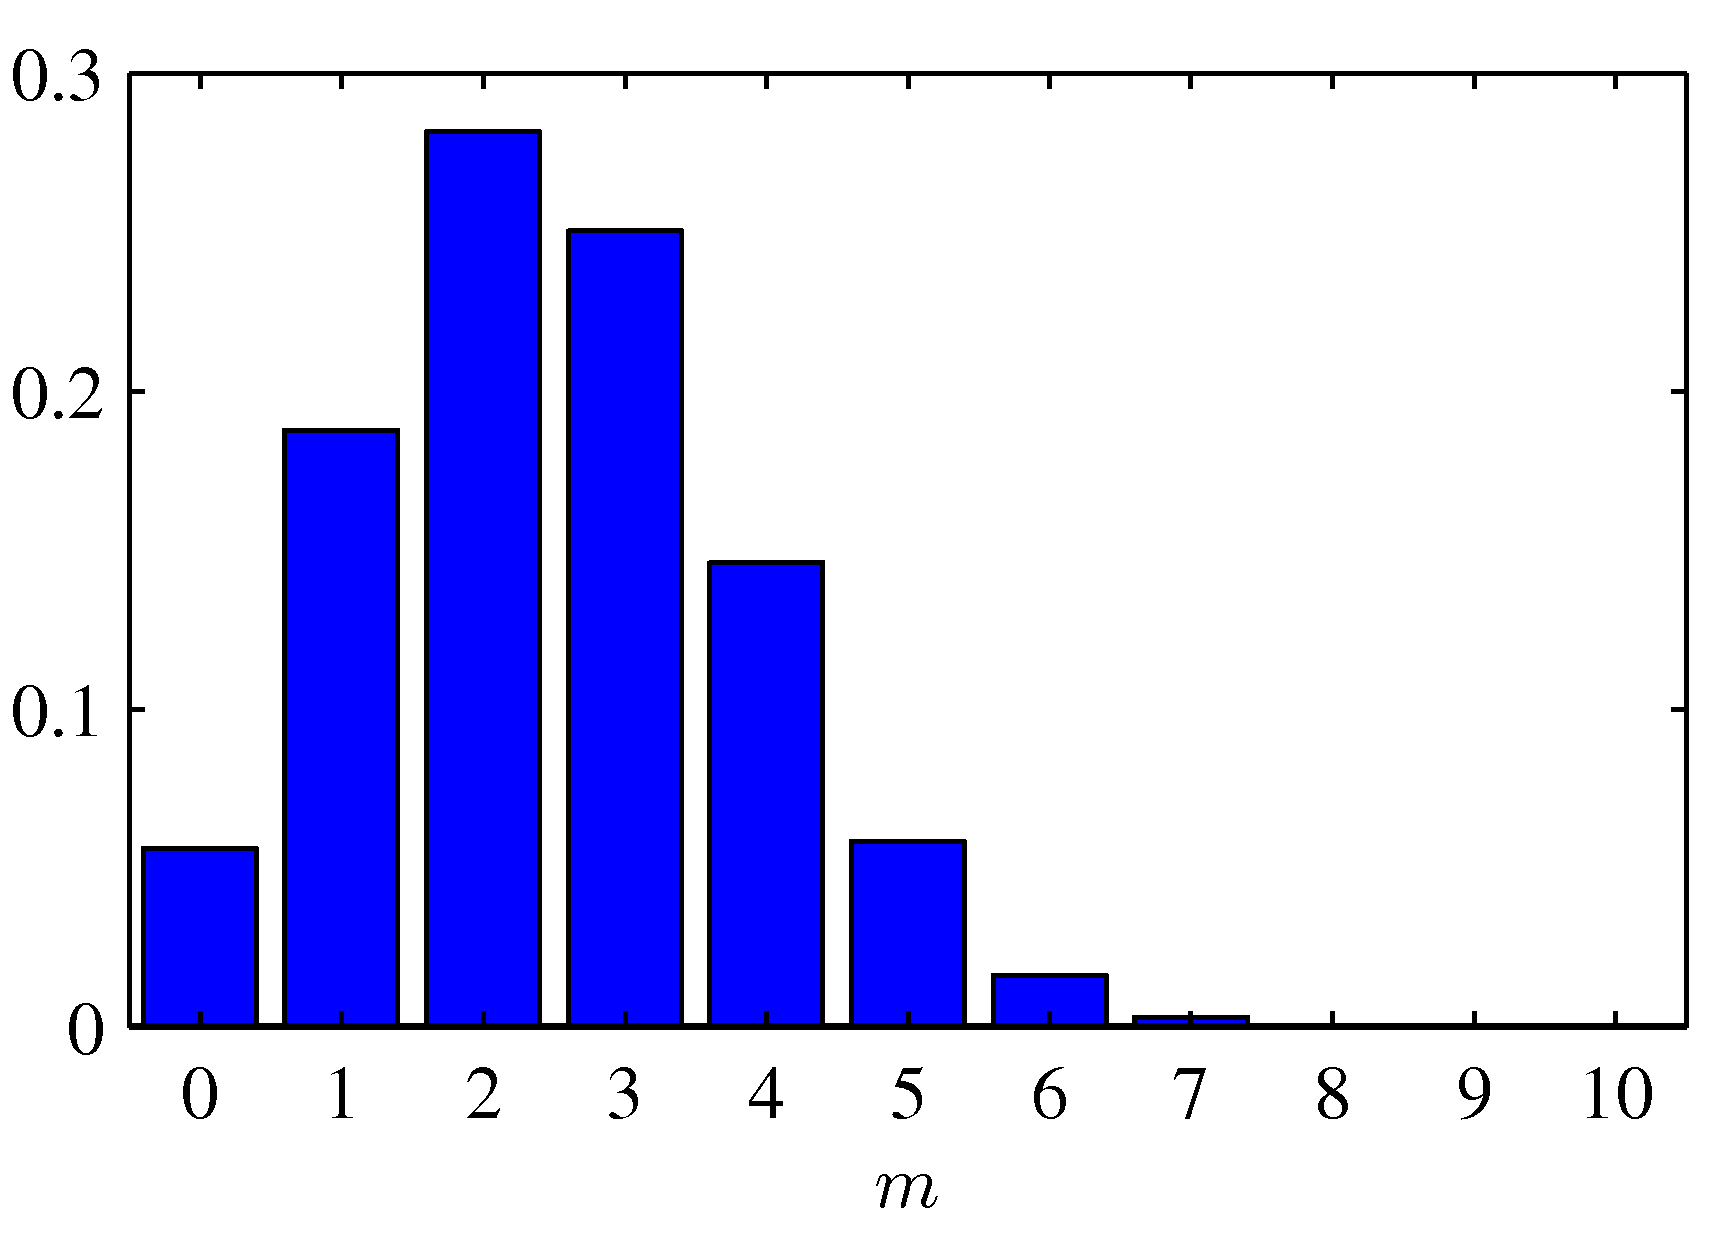
\includegraphics[scale=0.8]{Images/2-1.png}
		\captionsetup{font={small}}
		\caption{二项分布(2.9)在$N=10$和$\mu=0.25$时关于$m$的直方图。}
		\label{fig:2-1}
	\end{figure}
	\\
	\indent 二项分布的均值和方差可以通过习题1.10的结论求出,也就是对于独立事件而言,其总和的均值就是均值的总和,总和的方差就是方差的总和。由于$m=x_1+...+x_N$,而且数据集中每个元素的均值和方差都由(2.3)和(2.4)给出了,那么
	\begin{align}
		\mathbb{E}[m] \equiv \sum_{m=0}^{N}m \mathrm{Bin}(m|N,\mu) &= N\mu \\
		\mathrm{var}[m] \equiv \sum_{m=0}^N(m-\mathbb{E}[m])^2\mathrm{Bin}(m|N,\mu) &= N\mu(1-\mu)
	\end{align}
	这两个结果也可以直接计算得到。\textcolor{red}{\textbf{——习题 2.4}}
	}
	\subsection{beta分布}
	\textnormal{在(2.8)中我们已经看到了求伯努利分布参数$\mu$的最大似然的方法,所以在二项分布中参数$\mu$的最大似然是根据数据集中$x=1$的数据在数据集中所占的比例来确定的。我们已经发现了在较小的数据集上这种方法可能会造成过拟合的现象。为了对这个问题进行贝叶斯风格的处理,我们需要引入一个参数$\mu$的先验分布$p(\mu)$。在这里,我们需要的是一个比较简单,又有很多实用性质的先验分布。为了得到这个先验,我们首先注意到似然函数的形式是一系列因子$\mu^x(1-\mu)^{1-x}$的乘积。如果我们选择的是类似形式的先验,而先验分布与似然函数求乘积之后又和后验分布仅相差一个系数,那么后验分布就与先验分布具有相同的形式了。这样的性质称为共轭(conjugacy),在本章后面的内容中会看到共轭的相关案例。于是我们选择了这样的一个先验,起个名字叫做beta分布,形式为\\
	\begin{equation}
		\mathrm{Beta}(\mu|a,b)=\frac{\Gamma(a+b)}{\Gamma(a)\Gamma(b)}\mu^{a-1}(1-\mu)^{b-1}
	\end{equation}
	其中的$\Gamma(x)$为Gamma函数,定义详见(1.141)。(2.13)中的常数使beta分布满足归一化条件,\textcolor{red}{\textbf{——习题 2.5}}\ 也就是说
	\begin{equation}
		\int_0^1\mathrm{Beta}(\mu|a,b)\ \mathrm{d}\mu =1
	\end{equation}
	beta分布的均值和方差分别为\textcolor{red}{\textbf{——习题 2.6}}
	\begin{align}
		\mathbb{E}[\mu]&=\frac{a}{a+b} \\
		\mathrm{var}[\mu]&=\frac{ab}{(a+b)^2(a+b+1)}
	\end{align}
	其中的参数$a$和$b$被称为超参数(hyperparameters),因为它们把控着分布的参数$\mu$。如图2.2所示为超参数取不同值时的beta分布。
	\begin{figure}[ht]
		\begin{minipage}[t]{0.5\linewidth}
		\centering
		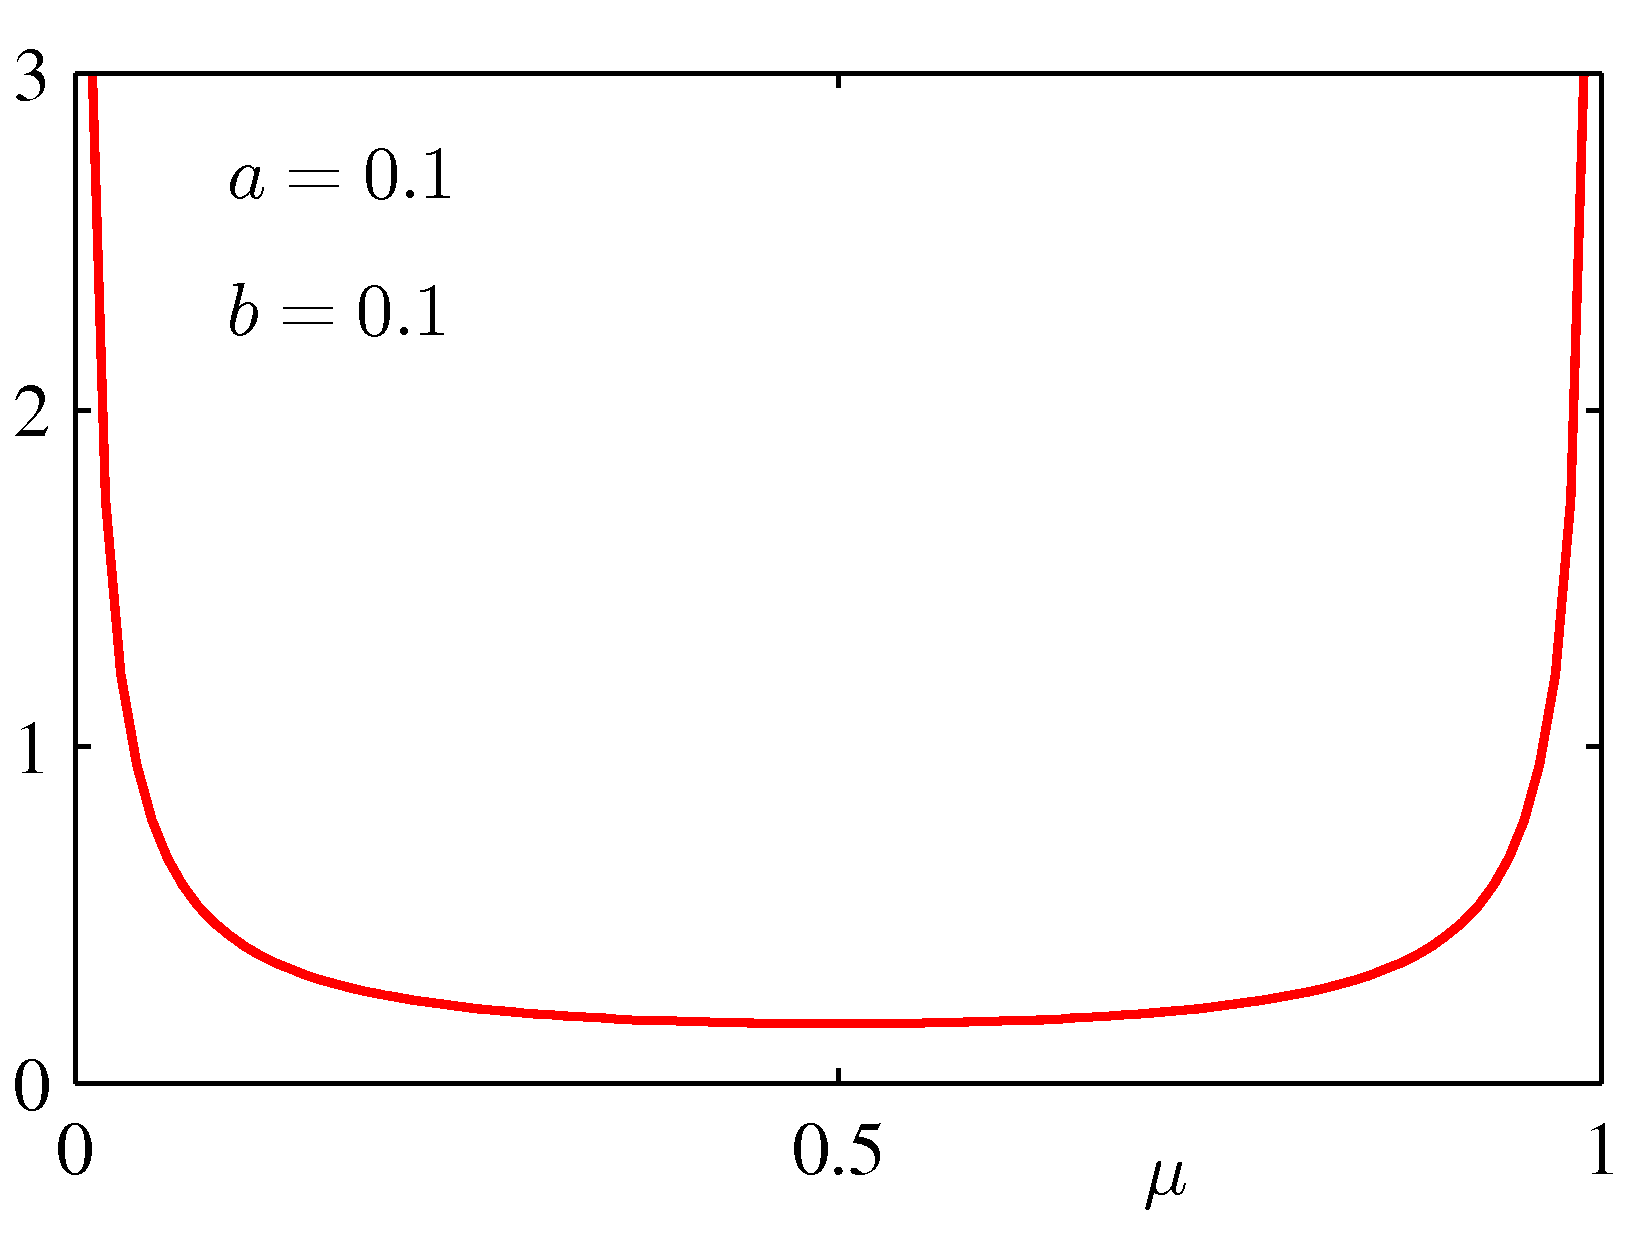
\includegraphics[scale=0.8]{Images/2-2a.png}
		\label{fig:2-2a}
		\end{minipage}
		\begin{minipage}[t]{0.5\linewidth}
		\centering
		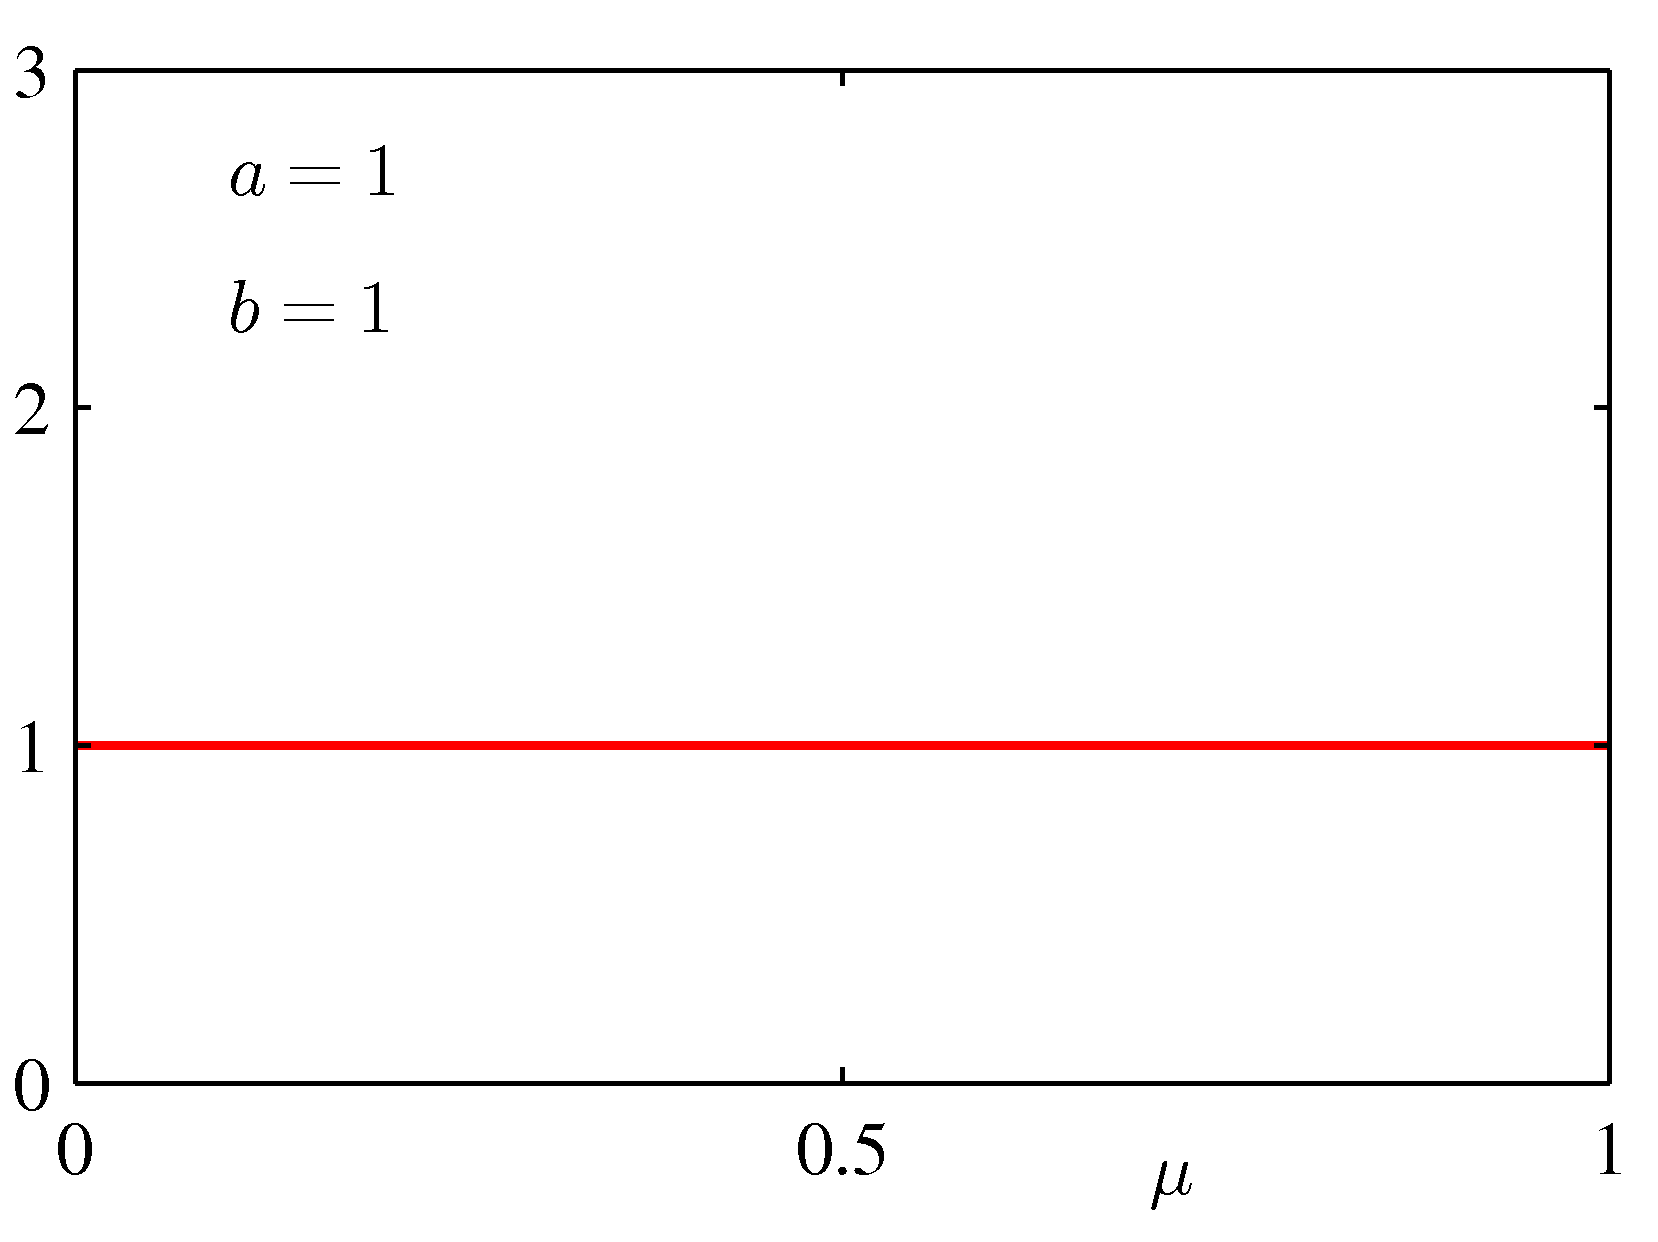
\includegraphics[scale=0.8]{Images/2-2b.png}
		\label{fig:2-2b}
		\end{minipage}\\
		\begin{minipage}[t]{0.5\linewidth}
		\centering
		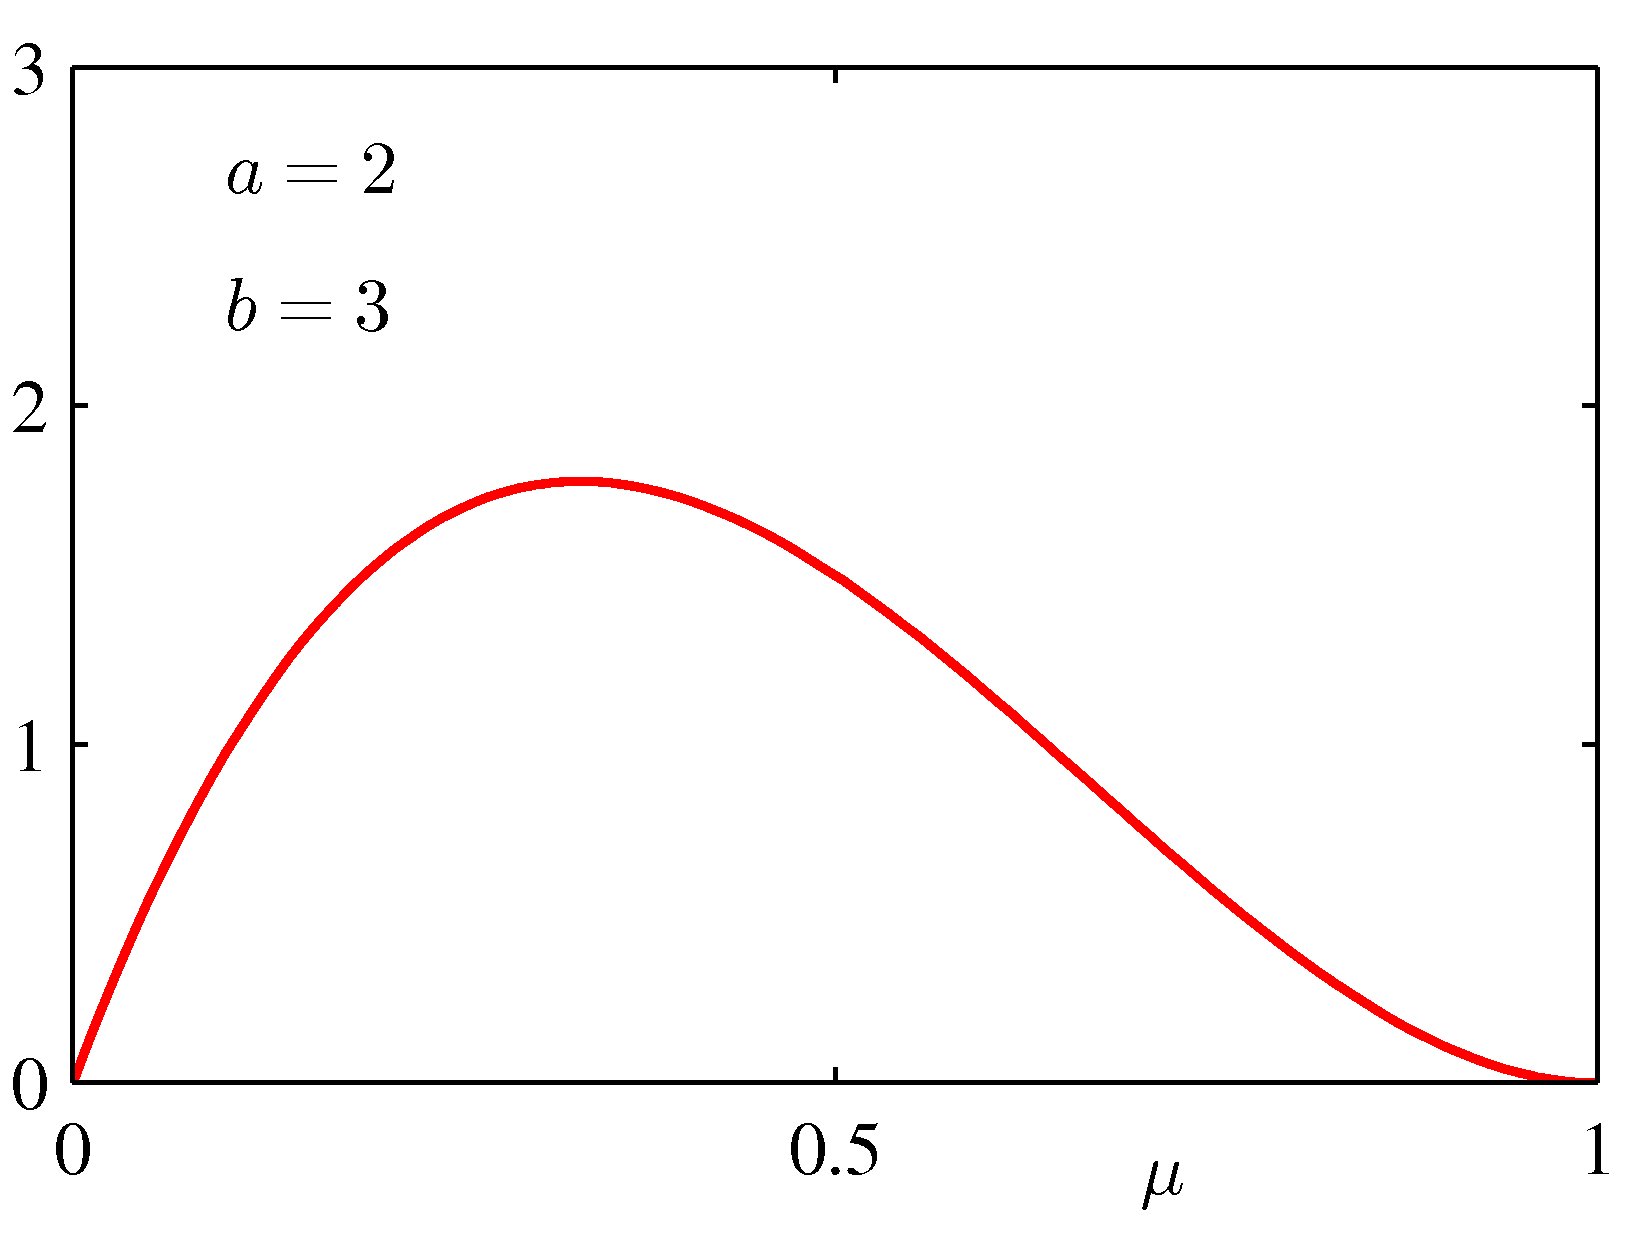
\includegraphics[scale=0.8]{Images/2-2c.png}
		\label{fig:2-2c}
		\end{minipage}
		\begin{minipage}[t]{0.5\linewidth}
		\centering
		\includegraphics[scale=0.8]{Images/2-2d.png}
		\label{fig:2-2d}
		\end{minipage}
		\captionsetup{font={small}}
		\caption{在不同的超参数$a$,$b$下,(2.13)中的beta分布$\mathrm{Beta}(\mu|a,b)$关于$\mu$的函数图像。}
	\end{figure}
	\\
	\indent 现在可以将beta分布(2.13)作为先验,乘以二项似然函数(2.9)并进行归一化,从而得到$\mu$的后验分布。仅保留与$\mu$相关的因子,可以看出后验分布为如下形式:
	\begin{equation}
		p(\mu|m,l,a,b) \propto \mu^{m+a-1}(1-\mu)^{l+b-1}
	\end{equation}
	其中$l=N-m$,所以就与背面朝上的次数挂上关系了。可以看出,作为$\mu$的函数,(2.17)的形式与先验分布的形式是相同的,也反映了先验分布与似然函数之间的共轭性质。实际上这就是另一个beta分布,通过与(2.13)做一下对比就可以写出其归一化常数:
	\begin{equation}
		p(\mu|m,l,a,b)=\frac{\Gamma(m+a+l+b)}{\Gamma(m+a)\Gamma(l+b)}\mu^{m+a-1}(1-\mu)^{l+b-1}
	\end{equation}
	\indent 可以看出,数据集会在先验分布转化为后验分布的过程中产生影响,如果$x=1$的观测数量为$m$,$x=0$的观测数量为$l$,那么$a$就会增加$m$,$b$会增加$l$。这就使得我们可以将超参数$a$和$b$比较简单地解释为$x=1$和$x=0$的有效数据量(effective number of observations)。注意,$a$和$b$可以不是整数。另外,如果我们还有后续的新数据,那么后验分布就可以成为下一步的先验分布。为了看清楚这一点,我们可以想象在每次数据观测之后都更新当前的后验分布,更新的方式为,将后验分布与新观测的似然函数相乘并进行归一化后,得到进一步修正的新后验分布。在每一步中,后验分布都是带有超参数$a$和$b$的beta分布,超参数$a$和$b$分别表示$x=1$和$x=0$的数量。如果有一个新的$x=1$加入进来,就直接将$a$值加上1即可,同理,如果有一个新的$x=0$加入进来,那就直接将$b$的值加上1。图2.3展示了这一过程,也就是获得一个新的数据时对分布进行的修正。
	\begin{figure}[ht]
	\centering
		\begin{minipage}[t]{0.3\linewidth}
		\centering
		\includegraphics[scale=0.8]{Images/2-3a.png}
		\label{fig:2-3a}
		\end{minipage}
		\begin{minipage}[t]{0.3\linewidth}
		\centering
		\includegraphics[scale=0.8]{Images/2-3b.png}
		\label{fig:2-3b}
		\end{minipage}
		\begin{minipage}[t]{0.3\linewidth}
		\centering
		\includegraphics[scale=0.8]{Images/2-3c.png}
		\label{fig:2-3c}
		\end{minipage}
		\captionsetup{font={small}}
		\caption{贝叶斯推断过程中的一次分布更新。先验beta分布的超参数$a=2$,$b=2$,似然函数如(2.9)所示,其中的$N=m=1$,也就是拿到了一个新的$x=1$的数据,于是后验beta分布的超参数就是$a=3$,$b=2$了。}
	\end{figure}
	\\
	\indent 可以看出,如果使用贝叶斯观点,那么可以自然而然地形成这种“顺序”(sequential)的学习方法。它与我们所选择的先验分布和似然函数无关,而是仅仅与数据的独立同分布假设相关。随着顺序方法的一步步推进,在每一步中都会利用单个或者小批量的数据,然后在使用下一个观测数据进行更新之前将它们废弃。举例而言,在实时学习的场合中,我们要在数据以稳定的数据流的形式到达之后对之逐一加以利用,而且要在全部数据到达之前进行预测。由于不需要将完整的数据集都存储或加载到内存中,所以顺序方法也经常应用于大型的数据集中。另外,最大似然方法实际上也可以转化为顺序框架的形式。\textcolor{red}{\textbf{——第2.3.5节}}\\
	\indent 如果我们的目标是尽可能准确地预测下一次试验的结果,那我们就必须对给定数据集$D$的条件下$x$的预测分布进行评价。根据概率论中的加法和乘法规则,有如下等式:
	\begin{equation}
		p(x=1|\mathcal{D})=\int_0^1p(x=1|\mu)p(\mu|\mathcal{D})\ \mathrm{d}\mu = \int_0^1 \mu p(\mu|\mathcal{D})\ \mathrm{d}\mu = \mathbb{E}[\mu|\mathcal{D}]
	\end{equation}
	利用(2.18)中的结果,结合(2.15)中的关于beta分布均值的结论,对于后验分布$p(\mu|\mathcal{D})$,有:
	\begin{equation}
		p(x=1|\mathcal{D})=\frac{m+a}{m+a+l+b}
	\end{equation}
	这个等式的意义很简单,实际上就是$x=1$的数据数量占数据总数的比例。需要注意的是,对于无限大的数据集,$m,l \rightarrow \infty$,(2.20)就退化成了(2.8)中的最大似然结果。我们即将看到,贝叶斯方法和最大似然方法的结果在数据集趋向于无限大时其实是一致的,这是一条非常重要的性质。而在有限数据集中,$\mu$的后验均值总是处于先验均值与最大似然结果之间,最大似然结果对应的是(2.7)所给出的事件相对频率。\textcolor{red}{\textbf{——习题 2.7}}\\
	\indent 从图2.2中可以看出,随着数据数量的增加,后验分布会变得越来越陡峭。也可以从(2.16)中看出一些端倪,当$a \rightarrow \infty$或$b \rightarrow \infty$时,方差会趋向于0。实际上,我们希望知道这是不是贝叶斯学习的一般属性之一,即当我们获得越来越多的数据之后,后验分布所代表的不确定性会不会逐步地下降。\\
	\indent 为了验证这一点,我们可以从频率域的角度来审视贝叶斯学习,并证明在一般情况下这个性质确实是成立的。让我们设想一个一般的贝叶斯推断问题,我们要根据数据集$\mathcal{D}$推断参数$\boldsymbol{\theta}$,其关系由联合分布$p(\boldsymbol{\theta},\mathcal{D})$来描述。以下结果\textcolor{red}{\textbf{——习题 2.8}}
	\begin{equation}
		\mathbb{E}_{\boldsymbol{\theta}}[\boldsymbol{\theta}]=\mathbb{E}_{\mathcal{D}}[\mathbb{E}_{\boldsymbol{\theta}}[\boldsymbol{\theta}|\mathcal{D}]]
	\end{equation}
	其中
	\begin{align}
		\mathbb{E}_{\boldsymbol{\theta}}[\boldsymbol{\theta}] &\equiv \int p(\boldsymbol{\theta})\boldsymbol{\theta}\ \mathrm{d}\boldsymbol{\theta} \\
		\mathbb{E}_{\mathcal{D}}[\mathbb{E}_{\boldsymbol{\theta}}[\boldsymbol{\theta}|\mathcal{D}]] &\equiv \int \left\{\int \boldsymbol{\theta} p(\boldsymbol{\theta}|\mathcal{D})\ \mathrm{d}\boldsymbol{\theta} \right\}p(\mathcal{D})\ \mathrm{d}\mathcal{D}
	\end{align}
	表明,基于全部数据取平均值的$\boldsymbol{\theta}$的后验均值与其先验均值相等。类似地,我们也可以证明
	\begin{equation}
		\mathrm{var}_{\boldsymbol{\theta}}[\boldsymbol{\theta}]=\mathbb{E}_{\mathcal{D}}[\mathrm{var}_{\boldsymbol{\theta}}[\boldsymbol{\theta}|\mathcal{D}]] + \mathrm{var}_{\mathcal{D}}[\mathbb{E}_{\boldsymbol{\theta}}[\boldsymbol{\theta}|\mathcal{D}]]
	\end{equation}
	等式(2.24)的等号左侧为$\boldsymbol{\theta}$的先验方差。在等号右侧,第一项为$\boldsymbol{\theta}$的平均后验方差,第二项衡量的是$\boldsymbol{\theta}$后验期望的方差。由于这个方差是个非负数,所以这个结果的含义是,在一般情况下,$\boldsymbol{\theta}$的后验方差小于先验方差。如果后验均值的方差比较大,那么方差减小的量会变得更大。不过需要注意的是,这个结论仅在一般情况下适用,对于很特殊的数据集,那么还是有可能出现后验方差大于先验方差的情况的。
	}
	\section{多项变量}
	\insertline
	\textnormal{
	\indent 二元变量可以描述变量有一种或者两种取值的情况。不过通常,我们面对的离散变量可能会有$K$种取值,且每种取值之间是互斥的。有很多方式来表达这样的变量,其中一种特别方便的办法叫做1-of-K方法,我们很快就会用到它。这个方法中,每个变量都表示为$K$维向量$x$,其中有且仅有一个分量$x_k=1$,其余均为0。于是,假设我们有个$K=6$的随机变量,而且要表示$x_3=1$的状态,那么直接可以写成
	\begin{equation}
		\bx=(0,0,1,0,0,0)^{\rmT}
	\end{equation}
	需要注意的是分量之和满足$\sum_{k=1}^K x_k=1$。如果我们将$x_k=1$的概率记为$\mu_k$,那么$\bx$的分布就是
	\begin{equation}
		p(\bx|\boldsymbol{\mu})=\prod_{k=1}^K \mu_k^{x_k}
	\end{equation}
	其中$\boldsymbol{\mu}=(\mu_1,...,\mu_K)^\rmT$,而且参数$\mu_k$满足条件$\mu_k \geqslant 0$和$\sum_k\mu_k=1$,因为它们表示的是概率。分布(2.26)可以看成是伯努利分布推广成的具有2个以上输出的形式。可以看出这个分布是归一化的:
	\begin{equation}
		\sum_{\bx}p(\bx|\boldsymbol{\mu})=\sum_{k=1}^K\mu_k=1
	\end{equation}
	以及
	\begin{equation}
		\mathbb{E}[\bx|\boldsymbol{\mu}]=\sum_{\bx}p(\bx|\boldsymbol{\mu})\bx = (\mu_1,...,\mu_K)^\rmT =\boldsymbol{\mu}
	\end{equation}
	\indent 现在对于一个含有$N$个独立观测的数据集$\mathcal{D}$,对应的似然函数为
	\begin{equation}
		p(\mathcal{D}|\boldsymbol{\mu})=\prod_{n=1}^N\prod_{k=1}^K \mu_k^{x_{nk}}=\prod_{k=1}^K\mu_k^{(\sum_nx_{nk})}=\prod_{k=1}^K \mu_k^{m_k}
	\end{equation}
	可以看出,似然函数对于这$N$个数据的依赖仅在于其中的$K$个值
	\begin{equation}
		m_k=\sum_nx_{nk}
	\end{equation}
	也就是$x_k=1$的数据数量。它们被称为分布中的充分统计量(sufficient statistics)。\textcolor{red}{\textbf{——第2.4节}}\\
	\indent 为了求出$\boldsymbol{\mu}$的最大似然解,我们需要对$\ln p(\mathcal{D}|\boldsymbol{\mu})$关于$\mu_k$求最大值,约束条件是$\mu_k$的总和必须为1。我们可以利用拉格朗日乘数$\lambda$计算\textcolor{red}{\textbf{——附录 E}}
	\begin{equation}
		\sum_{k=1}^Km_k \ln \mu_k + \lambda\left(\sum_{k=1}^K\mu_k-1\right)
	\end{equation}
	对(2.31)关于$\mu_k$求导并令导数为0,可以得到
	\begin{equation}
		\mu_k = -m_k/\lambda
	\end{equation}
	可以通过将(2.32)代入约束$\sum_k\mu_k$来求拉格朗日乘数$\lambda$,最后结果为$\lambda=-N$。于是我们可以得到如下形式的最大似然解
	\begin{equation}
		\mu_k^{\mathrm{ML}}=\frac{m_k}{N}
	\end{equation}
	很明显是在$N$项数据中$x_k=1$的数据所占的比例。\\
	\indent 接下来研究的是在给定参数$\boldsymbol{\mu}$和数据总数$N$的情况下$m_1,...,m_K$的联合分布。根据(2.29),其形式为
	\begin{equation}
		\mathrm{Mult}(m_1,m_2,...,m_K|\boldsymbol{\mu},N)=\left(\begin{matrix}N \\ m_1 m_2 ... m_K\end{matrix}\right)\prod_{k=1}^K\mu_k^{m_k}
	\end{equation}
	这就是多项分布(multinomial distribution)。其归一化常数是将$N$个目标分成大小为$m_1,...,m_K$的$K$组的方法数量:
	\begin{equation}
		\left(\begin{matrix}N \\ m_1m_2...m_K\end{matrix}\right)=\frac{N!}{m_1!m_2!...m_K!}
	\end{equation}
	需要注意的是,变量$m_k$满足
	\begin{equation}
		\sum_{k=1}^K m_k =N
	\end{equation}
	}
	\subsection{狄利克雷分布}
	\textnormal{现在我们来看一个先验分布族。这一族先验分布是多项分布(2.34)中参数$\{\mu_k\}$的先验分布。通过多项分布的形式可以看出,其共轭先验为
	\begin{equation}
		p(\boldsymbol{\mu}|\boldsymbol{\alpha}) \propto \prod_{k=1}^K \mu_k^{\alpha_k-1}
	\end{equation}
	其中的$0 \leqslant \mu_k \leqslant 1$,而且$\sum_k \mu_k=1$。$\alpha_1,...,\alpha_K$为分布的参数,记作$\boldsymbol{\alpha}=(\alpha_1,...,\alpha_K)^{\rmT}$。需要注意的是,由于求和常数,这个位于$\left\{\mu_k \right\}$空间中的分布局限于一个维数$K-1$的单型(simplex),图2.4所示的是$K=3$的情况。
	\begin{figure}[ht]
		\centering
		\includegraphics[scale=0.8]{Images/2-4.png}
		\captionsetup{font={small}}
		\caption{3个变量$\{\mu_1,\mu_2,\mu_3\}$的狄利克雷分布局限于如图所示的单型(即线性边界的流形)。这是限制条件$0 \leqslant \mu_k \leqslant 1$和$\sum_k\mu_k=1$所造成的。}
		\label{fig:2-4}
	\end{figure}
	\\
	\indent 该分布的归一化形式为
	\begin{equation}
		\mathrm{Dir}(\bfMu|\boldsymbol{\alpha})=\frac{\Gamma(\alpha_0)}{\Gamma(\alpha_1)...\Gamma(\alpha_K)}\prod_{k=1}^K\mu_k^{\alpha_k - 1}
	\end{equation}
	这就是狄利克雷分布(Dirichlet distribution)。其中,$\Gamma(x)$为Gamma函数,定义于(1.141),同时有
	\begin{equation}
		\alpha_0 = \sum_{k=1}^K \alpha_k
	\end{equation}
	在参数$\alpha_k$取不同的值时,单型上的狄利克雷分布如图2.5所示。
	\begin{figure}[ht]
	\centering
		\begin{minipage}[t]{0.3\linewidth}
		\centering
		\includegraphics[scale=0.8]{Images/2-5a.png}
		\label{fig:2-5a}
		\end{minipage}
		\begin{minipage}[t]{0.3\linewidth}
		\centering
		\includegraphics[scale=0.8]{Images/2-5b.png}
		\label{fig:2-5b}
		\end{minipage}
		\begin{minipage}[t]{0.3\linewidth}
		\centering
		\includegraphics[scale=0.8]{Images/2-5c.png}
		\label{fig:2-5c}
		\end{minipage}
		\captionsetup{font={small}}
		\caption{3个变量的狄利克雷分布,其中两个水平轴是单型平面的坐标,垂直轴表示概率密度值。左图中$\{\alpha_k\}=0.1$,中间的图中$\{\alpha_k\}=1$,右图中$\{\alpha_k\}=10$。}
	\end{figure}
	\\
	\indent 将先验(2.38)乘以似然函数(2.34),我们可以得到参数$\{\mu_k\}$的后验分布
	\begin{equation}
		p(\bfMu|\mathcal{D},\boldsymbol{\alpha}) \propto p(\calD|\bfMu)p(\bfMu|\bfAl) \propto \prod_{k=1}^K \mu_k^{\alpha_k+m_k-1}
	\end{equation}
	可以看出后验分布也是狄利克雷分布的形式,也就确定了狄利克雷分布是多项分布的共轭先验。于是可以通过与(2.38)做一下对比来求取归一化常数
	\begin{equation}
	\begin{split}
		p(\bfMu|\calD,\bfAl) &= \mathrm{Dir}(\bfMu|\bfAl+\mathbf{m}) \\
		&=\frac{\Gamma(\alpha_0+N)}{\Gamma(\alpha_1+m_1)...\Gamma(\alpha_K+m_K)}\prod_{k=1}^K\mu_k^{\alpha_k+m_k-1}
	\end{split}
	\end{equation}
	其中$\mathbf{m}=(m_1,...,m_K)^{\rmT}$。正如beta分布之于二项分布,我们也可以将狄利克雷先验中的参数$\alpha_k$解释为$x_k=1$的有效数据量。\\
	\indent 需要注意的是,二值变量既可以表示为二元变量并利用二项分布(2.9)进行建模,也可以表示为 1-of-2 变量并利用多项分布(2.34)进行建模,在这种情况下,多项分布中的$K=2$。
	}
	\section{高斯分布}
	\insertline\\
	\textnormal{
	\indent 高斯分布,也就是正态分布,是连续变量中广泛使用的分布模型。对于一元变量$x$,高斯分布的形式为
	\begin{equation}
		\mathcal{N}(x|\mu,\sigma^2)=\frac{1}{(2\pi\sigma^2)^{1/2}}\exp\left\{-\frac{1}{2\sigma^2}(x-\mu)^2\right\}
	\end{equation}
	其中$\mu$为均值,$\sigma^2$为方差。对于$D$维向量$\bx$,多元高斯分布的形式为
	\begin{equation}
		\calN(\bx|\bfMu,\bfSigma)=\frac{1}{(2\pi)^{D/2}}\frac{1}{|\bfSigma|^{1/2}}\exp\left\{-\frac{1}{2}(\bx-\bfMu)^{\rmT}\bfSigma^{-1}(\bx-\bfMu)\right\}
	\end{equation}
	其中$D$维向量$\bfMu$为均值,$D \times D$矩阵$\bfSigma$为协方差矩阵,$|\bfSigma|$为$\bfSigma$的行列式。\\
	\indent 高斯分布具有广泛的应用,而且可以从很多不同的角度来解读。举例而言,我们已经看到对于一个一元实值变量,使得熵取得最大值的分布就是高斯分布。\textcolor{red}{\textbf{——第1.6节}}\ 这个性质同样适用于多元高斯分布。\textcolor{red}{\textbf{——习题 2.14}}\\
	\indent 另外,在研究多元随机变量的求和时我们也会用到高斯分布。根据中心极限定理,在不太严苛的条件下,随着求和项数量的增加,一组随机变量的总和(当然这本身就是一个随机变量)会越来越趋近于一个高斯分布(Walker, 1969)。假设有$N$个变量$x_1,...,x_N$,每个变量都服从$[0,1]$上的均匀分布,那么均值就是$(x_1+...+x_N)/N$。对于较大的$N$,如图2.6所示,这个分布会趋近于高斯分布。在实际应用中,随着$N$的增加,分布向高斯分布收敛的速度会非常快。一个比较典型的结果是,二项分布(2.9)将在$N \rightarrow \infty$时趋向于高斯分布,因为二项分布实际上是定义在$m$上的分布,而$m$表示的是二值变量$x$在$N$次观测中的结果总数(详见图2.1中$N=10$的情况)。
	\begin{figure}[ht]
	\centering
		\begin{minipage}[t]{0.3\linewidth}
		\centering
		\includegraphics[scale=0.8]{Images/2-6a.png}
		\label{fig:2-6a}
		\end{minipage}
		\begin{minipage}[t]{0.3\linewidth}
		\centering
		\includegraphics[scale=0.8]{Images/2-6b.png}
		\label{fig:2-6b}
		\end{minipage}
		\begin{minipage}[t]{0.3\linewidth}
		\centering
		\includegraphics[scale=0.8]{Images/2-6c.png}
		\label{fig:2-6c}
		\end{minipage}
		\captionsetup{font={small}}
		\caption{当$N$取不同的值时,$N$个服从均匀分布的变量的均值直方图。可以看出随着$N$的增加,分布会趋近于高斯分布。}
	\end{figure}
	\\
	\indent 高斯分布具有很多重要的性质,我们很快就会详细地研究它们。于是乎,这一节会比前面的内容的技术含量更高,而且对矩阵的各种性质要求会比较高。\textcolor{red}{\textbf{——附录 C}}\ 尽管如此,我们还是强烈建议读者熟练掌握这一部分的内容,熟练操作高斯分布将会对后面章节中的复杂模型具有很大的帮助。请务必咬紧牙关,坚持下去。\\
	\indent 我们从高斯分布的几何形式开始。高斯分布中与$\bx$有关的部分是一个二次型
	\begin{equation}
		\Delta^2=(\bx-\bfMu)^{\rmT}\bfSigma^{-1}(\bx-\bfMu)
	\end{equation}
	这个二次型是出现在指数中的。$\Delta$表示的是$\bfMu$与$\bx$之间的马哈拉努比斯距离(即马氏距离,Mahalanobis distance,在后文中统一称为Mahalanobis距离),这个值将在$\bfSigma$为单位矩阵时退化为欧几里得距离。如果这个二次型为常数,那么这个高斯分布就是$\bx$空间中某个平面上的常数。\\
	\indent 首先,需要注意到矩阵$\bfSigma$一般可以认为是对称的,因为任何反对称分量都会在指数中消失。\textcolor{red}{\textbf{——习题 2.17} \ }对于协方差矩阵的特征向量方程
	\begin{equation}
		\bfSigma \mathbf{u}_i = \lambda_i \mathbf{u}_i
	\end{equation}
	其中$i=1,...,D$,由于$\bfSigma$是一个实对称矩阵,那么它的特征值一定是实数,其互异特征值对应的特征向量一定相互正交,\textcolor{red}{\textbf{——习题 2.18} \ }那么
	\begin{equation}
		\mathbf{u}_i^{\rmT} \mathbf{u}_j = I_{ij}
	\end{equation}
	其中$I_{ij}$为单位矩阵中的$\{i,j\}$元素,即
	\begin{equation}
		I_{ij}=\begin{cases}
		1,&\text{if}\ i=j \\
		0,&\text{otherwise}
		\end{cases}
	\end{equation}
	协方差矩阵可以表示为自身特征向量求和的形式\textcolor{red}{\textbf{——习题 2.19} \ }
	\begin{equation}
		\bfSigma=\sum_{i=1}^D\lambda_i\mathbf{u}_i\mathbf{u}_i^{\rmT}
	\end{equation}
	于是其逆矩阵$\bfSigma^{-1}$为
	\begin{equation}
		\bfSigma^{-1}=\sum_{i=1}^D\frac{1}{\lambda_i}\mathbf{u}_i\mathbf{u}_i^{\rmT}
	\end{equation}
	将(2.49)代入(2.44),二次型就变成了
	\begin{equation}
		\Delta^2=\sum_{i=1}^D\frac{y_i^2}{\lambda_i}
	\end{equation}
	其中
	\begin{equation}
		y_i=\mathbf{u}_i^{\rmT}(\bx - \bfMu)
	\end{equation}
	我们可以将$\{y_i\}$看成是正交向量$\mathbf{u}_i$下的新坐标系,当然,它是从原始的$x_i$坐标通过平移旋转得到的。构建向量$\mathbf{y}=(y_1,...,y_D)^{\rmT}$,可得
	\begin{equation}
		\mathbf{y}=\mathbf{U}(\mathbf{x}-\bfMu)
	\end{equation}
	其中的$\mathbf{U}$是以$\mathbf{u}_i^{\rmT}$为行的矩阵。根据(2.46),$\mathbf{U}$为正交矩阵,即$\mathbf{U}\mathbf{U}^{\rmT}=\mathbf{I}$,同时$\mathbf{U}^{\rmT}\mathbf{U}=\mathbf{I}$,其中$\mathbf{I}$为单位矩阵。\textcolor{red}{\textbf{——附录 C} \ }\\
	\indent 当(2.50)为常数时,该二次型将是某平面上的常数,则高斯概率密度也是常数。如果所有的特征值$\lambda_i$均为正数,该平面就是椭球面,其中心为$\bfMu$,轴的方向为$\mathbf{u}_i$,轴长的缩放因子为$\lambda_i^{1/2}$,如图2.7所示。
	\begin{figure}[ht]
		\centering
		\includegraphics[scale=0.8]{Images/2-7.png}
		\captionsetup{font={small}}
		\caption{图中红色的曲线表示的是二维空间$\bx=(x_1,x_2)$的常数概率分布椭球面,对应的是$\bx=\bfMu$处的概率密度为$\exp{-1/2}$。椭圆的两条轴是由协方差矩阵的特征向量$\mathbf{u}_i$得到的,其对应的特征值为$\lambda_i$。}
		\label{fig:2-7}
	\end{figure}
	\\
	\indent 高斯分布要求其协方差矩阵的特征值$\lambda_i$严格为正数,否则分布就不能归一化。特征值严格为正的矩阵称为正定矩阵。在第12章中,我们会遇到具有0特征值的高斯分布,这种情况下的分布是奇异的,而且被限制在了低维的子空间中。如果所有的特征值都是非负的,那么协方差矩阵就是半正定矩阵。\\
	\indent 现在我们来研究新坐标$y_i$下的高斯分布。在$\bx$变换成$\mathbf{y}$的过程中,有雅可比矩阵$\mathbf{J}$:
	\begin{equation}
		J_{ij}=\frac{\partial x_i}{\partial y_i}=U_{ji}
	\end{equation}
	其中的$U_{ji}$为矩阵$\mathbf{U}^{\rmT}$的元素。根据矩阵$\mathbf{U}$的对称性,可以看出雅可比矩阵行列式的平方为
	\begin{equation}
		|\mathbf{J}|^2 = |\mathbf{U}^{\rmT}|^2 = |\mathbf{U}^{\rmT}||\mathbf{U}|=|\mathbf{U}^{\rmT}\mathbf{U}|=|\mathbf{I}|=1
	\end{equation}
	于是$|\mathbf{J}|=1$,而且协方差矩阵的行列式$|\bfSigma|$可以写成特征值乘积的形式:
	\begin{equation}
		|\bfSigma|^{1/2}=\prod_{j=1}^D\lambda_j^{1/2}
	\end{equation}
	于是在$y_i$坐标系中,高斯分布的形式为
	\begin{equation}
		p(\mathbf{y})=p(\mathbf{x})|\mathbf{J}| = \prod_{j=1}^D\frac{1}{(2\pi\lambda_j)^{1/2}}\exp\left\{-\frac{y_j^2}{2\lambda_j}\right\}
	\end{equation}
	事实上就是$D$个相互独立的一元高斯分布的乘积。于是特征向量定义了一个经过平移和旋转的新坐标系,在这个坐标系中,联合概率分布可以分解为若干独立分布的乘积。在$\mathbf{y}$坐标系中的积分为
	\begin{equation}
		\int p(\mathbf{y})\ \mathrm{d}\mathbf{y} = \prod_{j=1}^D\int_{-\infty}^{\infty}\frac{1}{(2\pi\lambda_j)^{1/2}}\exp \left\{-\frac{y_j^2}{2\lambda_j}\right\}\ \mathrm{d}y_i=1
	\end{equation}
	其中我们利用了(1.48)中一元高斯函数归一化的结论。这也验证了多元高斯分布(2.43)确实是归一化的。\\
	\indent 我们现在来研究一下高斯分布的矩,从而解释一下参数$\bfMu$和$\bfSigma$的含义。在高斯分布下$\bx$的期望为
	\begin{equation}
	\begin{split}
		\mathbb{E}[\bx] &= \frac{1}{(2\pi)^{D/2}} \frac{1}{|\bfSigma|^{1/2}}\int \exp \left\{-\frac{1}{2}(\bx-\bfMu)^{\rmT}\bfSigma^{-1}(\bx-\bfMu)\right\}\bx \ \mathrm{d}\bx \\
		&=\frac{1}{(2\pi)^{D/2}} \frac{1}{|\bfSigma|^{1/2}}\int \exp \left\{-\frac{1}{2}\mathbf{z}^{\rmT}\bfSigma^{-1}\mathbf{z}\right\}(\mathbf{z}+\bfMu) \ \mathrm{d}\mathbf{z}
	\end{split}
	\end{equation}
	其中进行了变量的替换$\mathbf{z}=\bx-\bfMu$。此时注意到积分号里的指数部分是关于$\mathbf{z}$的偶函数,而积分区间是$(-\infty,\infty)$,很明显是对称区间,而带上$(\mathbf{z}+\bfMu)$中$\mathbf{z}$的那一项变成了奇函数,于是在积分之后就消失了,再利用一下高斯分布的归一化条件,最后的结果为
	\begin{equation}
		\mathbb{E}[\bx]=\bfMu
	\end{equation}
	所以$\bfMu$就是高斯分布的均值。\\
	\indent 下面研究高斯分布的二阶矩。在一元变量的情况下,要计算的二阶矩为$\mathbb{E}[x^2]$;而对于多元高斯分布,二阶矩有$D^2$个,分别由$\mathbb{E}[x_i x_j]$给出,可以写成矩阵的形式$\mathbb{E}[\bx\bx^{\rmT}]$。这个矩阵实际上就是
	\[
	\begin{split}
		\mathbb{E}[\bx\bx^{\rmT}]&=\frac{1}{(2\pi)^{D/2}}\frac{1}{|\bfSigma|^{1/2}}\int \exp\left\{-\frac{1}{2}(\bx-\bfMu)^{\rmT}\bfSigma^{-1}(\bx-\bfMu)\right\}\bx \bx^{\rmT}\ \mathrm{d}\bx \\
		&=\frac{1}{(2\pi)^{D/2}}\frac{1}{|\bfSigma|^{1/2}}\int \exp\left\{-\frac{1}{2}\mathbf{z}^{\rmT}\bfSigma^{-1}\mathbf{z}\right\}(\mathbf{z}+\bfMu) (\mathbf{z}+\bfMu)^{\rmT}\ \mathrm{d}\mathbf{z}
	\end{split}
	\]
	其中再次用到了变量替换$\mathbf{z}=\bx-\bfMu$。需要注意的是,交叉项$\bfMu\mathbf{z}^{\rmT}$和$\mathbf{z}\bfMu^{\rmT}$会由于对称性而消失。$\bfMu\bfMu^{\rmT}$为常数,所以可以提到积分号外面,由于高斯分布是归一化的,所以它是一个单位矩阵。对于包含有$\mathbf{z}\mathbf{z}^{\rmT}$的那一项,再次根据(2.45)对协方差矩阵利用其互异的特征向量进行展开,于是有
	\begin{equation}
		\mathbf{z}=\sum_{j=1}^Dy_j\mathbf{u}_j
	\end{equation}
	其中$y_j=\mathbf{u}_j^{\rmT}\mathbf{z}$,于是有
	\begin{equation}
	\begin{split}
		&\frac{1}{(2\pi)^{D/2}}\frac{1}{|\bfSigma|^{1/2}}\int \exp \left\{-\frac{1}{2}\mathbf{z}^{\rmT}\bfSigma^{-1}\mathbf{z}\right\}\mathbf{z}\mathbf{z}^{\rmT}\ \mathrm{d}\mathbf{z}\\
		= &\frac{1}{(2\pi)^{D/2}}\frac{1}{|\bfSigma|^{1/2}}\sum_{i=1}^D \sum_{j=1}^D \mathbf{u}_i\mathbf{u}_j^{\rmT}\int \exp\left\{-\sum_{k=1}^D \frac{y_k^2}{2\lambda_k}\right\}y_iy_j\ \mathrm{d}\mathbf{y}\\
		= &\sum_{i=1}^D\mathbf{u}_i\mathbf{u}_i^{\rmT}\lambda_i = \bfSigma
	\end{split}
	\end{equation}
	其中使用了特征向量方程(2.45),并利用了一条性质:等号右侧的积分中,根据对称性,除非$i=j$,否则全部为0。最后一行的计算我们利用了结论(1.50)和(2.55),以及(2.48)。于是就有
	\begin{equation}
		\mathbb{E}[\bx\bx^{\rmT}]=\bfMu\bfMu^{\rmT}+\bfSigma
	\end{equation}
	\indent 对于一元随机变量,我们在定义方差之前要减去均值。类似地,对于多元变量的情况,我们也要减掉均值,从而得到随机变量$\bx$的协方差:
	\begin{equation}
		\mathrm{cov}[\bx]=\mathbb{E}\left[(\bx-\mathbb{E}[\bx])(\bx-\mathbb{E}[\bx]^{\rmT})\right]
	\end{equation}
	对于高斯分布,我们将$\mathbb{E}[\bx]=\bfMu$和(2.62)一同代入,得到
	\begin{equation}
		\mathrm{cov}[\bx]=\bfSigma
	\end{equation}
	由于参数$\bfSigma$控制了高斯分布下$\bx$的协方差,所以被称为协方差矩阵。\\
	\indent 尽管高斯分布(2.43)是广泛应用的概率密度模型,但它也具有很多明显的局限性。分布中自由参数的数量就是个问题,随便一个对称的协方差矩阵$\bfSigma$就有$D(D+1)/2$个独立参数,另外在$\bfMu$中还有另外$D$个,加起来足足有$D(D+3)/2$个独立参数。对于较大的$D$,独立参数的数量会随着$D$的增加呈平方型增长,求这样的大矩阵的乘积和逆,计算压力相当大,甚至可能是无解的。解决这个问题的方法之一,是限制协方差矩阵的形式。对于协方差矩阵为对角阵的情况,$\bfSigma=\mathrm{diag}(\sigma_i^2)$,于是概率密度模型中独立参数的数量为$2D$。其对应的常数概率密度的轮廓线为轴对称的椭球面。要是更严格一些,我们可以限制协方差矩阵为常数与单位矩阵的乘积,即$\bfSigma=\sigma^2 \mathbf{I}$,也就是协方差各向同性(isotropic),这样的话模型中独立参数的数量为$D+1$,椭球面也就变成了球面。一般、对角和各项同性三种协方差矩阵对应的概率密度如图2.8所示。不幸的是,尽管我们通过这样的方法限制了分布的自由度,使得协方差矩阵的逆求起来更加方便和快捷,但这样的做法也严重限制了概率密度的形式,同时也限制了模型抓住数据中最有用内容的能力。
	\begin{figure}[ht]
	\centering
		\begin{minipage}[t]{0.3\linewidth}
		\centering
		\includegraphics[scale=0.8]{Images/2-8a.png}
		\label{fig:2-8a}
		\end{minipage}
		\begin{minipage}[t]{0.3\linewidth}
		\centering
		\includegraphics[scale=0.8]{Images/2-8b.png}
		\label{fig:2-8b}
		\end{minipage}
		\begin{minipage}[t]{0.3\linewidth}
		\centering
		\includegraphics[scale=0.8]{Images/2-8c.png}
		\label{fig:2-8c}
		\end{minipage}
		\captionsetup{font={small}}
		\caption{二维高斯分布的常数概率密度轮廓线,(a)为一般情况;(b)为协方差矩阵为对角矩阵的情况,图中椭圆的两轴分别与两个坐标轴平行;(c)为协方差矩阵与单位矩阵成比例的情况,前几个图中的椭圆变成了圆。}
	\end{figure}
	\\
	\indent 高斯分布的另一个重要限制是,这个分布是单峰的——也就是只有一个最大值。于是高斯分布对于多峰分布的拟合自然显得力不从心。所以,作为一个带有很多参数的分布,高斯分布很灵活,但又有可能因为自身能够有效拟合的分布太少,而在应用中受到严重的限制。我们会在后文中介绍隐变量(latent variables)时解决以上的两个问题。特别地,如果将离散隐变量放到高斯混合模型中,将会得到一个很大的多峰分布族,我们将在第2.3.9节中介绍这个内容。类似地,在第12章中即将介绍的连续隐变量将使我们可以得到自由参数的数量可以由数据空间的维数$D$独立控制,又可以获取数据集里的核心内容的模型。实际上,这两个方法是可以联合在一起的,可以通过它们得到种类繁多的分层模型,在实际应用中可以广泛使用。举例而言,马尔科夫随机场(Markov random field)的高斯形态广泛应用于图像的概率模型中。它其实是一个像素空间中的高斯分布,但引入了能够反映像素空间组织结构的内容,从而处理起来更加方便。类似地,线性动态系统(linear dynamical system)可以用于时序数据的建模,比如说追踪,其实线性动态系统同样是建立在大量观测变量和隐变量上的联合高斯分布,所以同样可以得到有效的应对。为了表示这些复杂分布的形式和属性,我们会用到一种强大的框架——概率图模型,相关内容将在第8章中进行介绍。
	}
	\subsection{条件高斯分布}
	\textnormal{
	多元高斯分布具有一个很重要的性质,如果两组变量服从联合高斯分布,那么给定其中一组的条件下另一组的条件分布同样也是高斯分布,而且对两组变量的任意一组求边缘分布,得到的分布同样也是高斯分布。\\
	\indent 首先研究一下条件分布的情况。假设$\bx$是一个$D$维向量,服从高斯分布$\mathcal{N}(\bx|\bfMu,\bfSigma)$。现在将$\bx$拆分成两个相互独立的子集$\bx_a$和$\bx_b$,一般地,我们可以将$\bx_a$设置为$\bx$的前$M$个分量,而$\bx_b$则是$\bx$的后$D-M$个分量。于是
	\begin{equation}
		\bx = \left(\begin{matrix}\bx_a \\ \bx_b \end{matrix}\right)
	\end{equation}
	同样地将均值向量$\bfMu$对应拆开:
	\begin{equation}
		\bfMu = \left(\begin{matrix} \bfMu_a \\ \bfMu_b \end{matrix}\right)
	\end{equation}
	以及协方差矩阵:
	\begin{equation}
		\bfSigma=\left(\begin{matrix} \bfSigma_{aa} & \bfSigma_{ab} \\ \bfSigma_{ba} & \bfSigma_{bb} \end{matrix}\right)
	\end{equation}
	根据协方差矩阵的对称性$\bfSigma^{\rmT}=\bfSigma$,$\bfSigma_{aa}$和$\bfSigma_{bb}$都是对称矩阵,以及$\bfSigma_{ba}=\bfSigma_{ab}^{\rmT}$。\\
	\indent 在很多情况下,利用协方差矩阵的逆矩阵会更方便一些:
	\begin{equation}
		\boldsymbol{\Lambda} \equiv \bfSigma^{-1}
	\end{equation}
	这就是精度矩阵(precision matrix)。实际上,高斯分布的一些性质用协方差矩阵表示会比较方便,但还有很多性质用精度矩阵表示会更加方便。于是再多关注一下精度矩阵的拆分形式:
	\begin{equation}
		\boldsymbol{\Lambda}=\left(\begin{matrix}\boldsymbol{\Lambda}_{aa} & \boldsymbol{\Lambda}_{ab} \\ \boldsymbol{\Lambda}_{ba} & \boldsymbol{\Lambda}_{bb}\end{matrix}\right)
	\end{equation}
	拆分的形式也是对应着(2.65)中$\bx$的拆分形式的。由于对称矩阵的逆矩阵仍然是对称矩阵,\textcolor{red}{\textbf{——习题 2.22\ }}可以看出$\boldsymbol{\Lambda}_{aa}$和$\boldsymbol{\Lambda}_{bb}$为对称矩阵,以及$\boldsymbol{\Lambda}_{ab}^{\rmT}=\boldsymbol{\Lambda}_{ba}$。不过这里需要指出一个问题,$\bfLambda_{aa}$绝不仅仅是$\bfSigma_{aa}$求逆那么简单。我们现在就来研究一下分块矩阵的逆矩阵及其分块的逆矩阵。\\
	\indent 就从求取条件分布$p(\bx_a|\bx_b)$的表达式开始。根据概率的乘法规则,这个条件分布可以根据联合分布$p(\bx)=p(\bx_a,\bx_b)$求出,只需要将$\bx_b$设为固定值并进行归一化,最后就可以得到给定$\bx_b$的条件下$\bx_a$的概率分布。不过,与其按部就班地计算,我们不如先利用一下高斯分布中指数项里的二次型(2.44)的特殊性,然后再做归一化,这样可以更快地得到结果。根据(2.65)、(2.66)和(2.69)中的分块,可以得到
	\begin{equation}
	\begin{split}
		-\frac{1}{2}&(\bx-\bfMu)^{\rmT}\bfSigma^{-1}(\bx-\bfMu) = \\
		&-\frac{1}{2}(\bx_a-\bfMu_a)^{\rmT}\bfLambda_{aa}(\bx_a-\bfMu_a)-\frac{1}{2}(\bx_a-\bfMu_a)^{\rmT}\bfLambda_{ab}(\bx_b-\bfMu_b) \\ &-\frac{1}{2}(\bx_b-\bfMu_b)^{\rmT}\bfLambda_{ba}(\bx_a-\bfMu_a)-\frac{1}{2}(\bx_b-\bfMu_b)^{\rmT}\bfLambda_{bb}(\bx_b-\bfMu_b)
	\end{split}
	\end{equation}
	可以看出这是一个关于$\bx_a$的函数,而且同样是一个二次型,于是对应的条件分布$p(\bx_a|\bx_b)$也是一个高斯分布。由于这个分布完全由其均值和协方差确定,于是我们只需要根据(2.70)确定$p(\bx_a|\bx_b)$的均值和方差就可以确定整个分布了。\\
	\indent 对于高斯分布,“完成平方项”是一个相当常见的操作。在给定了高斯分布指数项中的二次型后,据此确定分布的均值和方差。这个问题可以这样解决,首先注意到高斯分布$\mathcal{N}(\bx|\bfMu,\bfSigma)$可以写成
	\begin{equation}
		-\frac{1}{2}(\bx-\bfMu)^{\rmT}\bfSigma^{-1}(\bx-\bfMu)=-\frac{1}{2}\bx^{\rmT}\bfSigma^{-1}\bx + \bx^{\rmT}\bfSigma^{-1}\bfMu + \mathrm{const}
	\end{equation}
	其中“const”表示的是与$\bx$无关的项,并利用了$\bfSigma$的对称性。所以对于一个一般的二次型,如果我们将它拆分成(2.71)的形式,那么就可以令$\bx$二次项的系数矩阵为协方差矩阵的逆矩阵$\bfSigma^{-1}$,令$\bx$一次项的系数向量为$\bfSigma^{-1}\bfMu$,于是就可以确定$\bfMu$了。\\
	\indent 现在我们用这个方法求取条件高斯分布$p(\bx_a|\bx_b)$,其指数项中的二次型就是(2.70)。我们用$\bfMu_{a|b}$表示均值,$\bfSigma_{a|b}$表示方差,将(2.70)看作是$\bx_a$的函数,将$\bx_b$看作是常数,对于$\bx_a$的二次项,其形式为
	\begin{equation}
		-\frac{1}{2}\bx_a^{\rmT}\bfLambda_{aa}\bx_a
	\end{equation}
	于是马上得到$p(\bx_a|\bx_b)$的协方差矩阵为
	\begin{equation}
		\bfSigma_{a|b}=\bfLambda_{aa}^{-1}
	\end{equation}
	对于(2.70)中$\bx_a$的一次项,
	\begin{equation}
		\bx_a^{\rmT}\{\bfLambda_{aa}\bfMu_a - \bfLambda_{ab}(\bx_b-\bfMu_b)\}
	\end{equation}
	其中用到了$\bfLambda_{ba}^{\rmT}=\bfLambda_{ab}$。根据(2.71),这个表达式中$\bx_a$的系数一定等于$\bfSigma_{a|b}^{-1}\bfMu_{a|b}$,于是根据(2.73),
	\begin{equation}
	\begin{split}
		\bfMu_{a|b} &= \bfSigma_{a|b}\{\bfLambda_{aa}\bfMu_a-\bfLambda_{ab}(\bx_b-\bfMu_b)\} \\
		&= \bfMu_a-\bfLambda_{aa}^{-1}\bfLambda_{ab}(\bx_b-\bfMu_b)
	\end{split}
	\end{equation}
	\indent (2.73)和(2.75)是根据原始的联合分布$p(\bx_a,\bx_b)$的精度矩阵的分块形式确定的,我们也可以对协方差矩阵进行分块得到这样的结果。为了完成这一点,我们利用如下的分块矩阵的逆矩阵的恒等式:
	\begin{equation}
		\left(\begin{matrix}\mathbf{A} & \mathbf{B} \\ \mathbf{C} & \mathbf{D} \end{matrix}\right)^{-1}=\left(\begin{matrix}\mathbf{M} & -\mathbf{MBD}^{-1} \\ -\mathbf{D}^{-1}\mathbf{CM} & \mathbf{D}^{-1}+\mathbf{D}^{-1}\mathbf{CMBD}^{-1}\end{matrix}\right)
	\end{equation}
	其中定义了
	\begin{equation}
		\mathbf{M}=(\mathbf{A}-\mathbf{BD}^{-1}\mathbf{C})^{-1}
	\end{equation}
	\textcolor{red}{\textbf{译者注:所以完整的矩阵为:}
	\[
		\left(\begin{matrix}\mathbf{A} & \mathbf{B} \\ \mathbf{C} & \mathbf{D} \end{matrix}\right)^{-1}=\left(\begin{matrix}(\mathbf{A}-\mathbf{BD}^{-1}\mathbf{C})^{-1} & -\mathbf{MBD}^{-1} \\ -\mathbf{D}^{-1}\mathbf{C}(\mathbf{A}-\mathbf{BD}^{-1}\mathbf{C})^{-1} & \mathbf{D}^{-1}+\mathbf{D}^{-1}\mathbf{C}(\mathbf{A}-\mathbf{BD}^{-1}\mathbf{C})^{-1}\mathbf{BD}^{-1}\end{matrix}\right)
	\]}
	其中的$\mathbf{M}^{-1}$就是(2.76)等号左侧的矩阵关于矩阵块$\mathbf{D}$的舒尔补(Schur complement)。根据定义,
	\begin{equation}
		\left(\begin{matrix}\bfSigma_{aa} & \bfSigma_{ab} \\ \bfSigma_{ba} & \bfSigma_{bb}\end{matrix}\right)^{-1} = \left(\begin{matrix}\bfLambda_{aa} & \bfLambda_{ab} \\ \bfLambda_{ba} & \bfLambda_{bb}\end{matrix}\right)
	\end{equation}
	以及根据(2.76),可以得到
	\begin{align}
		\bfLambda_{aa}&=(\bfSigma_{aa}-\bfSigma_{ab}\bfSigma_{bb}^{-1}\bfSigma_{ba})^{-1}\\
		\bfLambda_{ab}&=-(\bfSigma_{aa}-\bfSigma_{ab}\bfSigma_{bb}^{-1}\bfSigma_{ba})^{-1}\bfSigma_{ab}\bfSigma_{bb}^{-1}
	\end{align}
	根据这些,我们可以确定条件分布$p(\bx_a|\bx_b)$的均值和协方差的表达式
	\begin{align}
		\bfMu_{a|b}&=\bfMu_a + \bfSigma_{ab}\bfSigma_{bb}^{-1}(\bx_b-\bfMu_b) \\
		\bfSigma_{a|b}&=\bfSigma_{aa}-\bfSigma_{ab}\bfSigma_{bb}^{-1}\bfSigma_{ba}
	\end{align}
	通过对比(2.73)和(2.82),可以看出用精度矩阵表示条件分布$p(\bx_a|\bx_b)$比协方差矩阵更加简单。需要注意的是,(2.81)中条件分布$p(\bx_a|\bx_b)$的均值是关于$\bx_b$的线性函数,(2.82)中给出的协方差与$\bx_b$无关。这是线性高斯模型(linear-Gaussian model)的典型案例之一。\textcolor{red}{\textbf{——第8.1.4节}}
	}
	\subsection{边缘高斯分布}
	\textnormal{
	我们已经看到,如果联合分布$p(\bx_a, \bx_b)$为高斯分布,那么条件分布$p(\bx_a|\bx_b)$一定也是一个高斯分布。现在我们转向边缘分布的讨论,也就是
	\begin{equation}
		p(\bx_a)=\int p(\bx_a,\bx_b)\ \mathrm{d}\bx_b
	\end{equation}
	我们很快会发现它也是一个高斯分布。和之前一样,我们的注意力仍然将集中在联合分布中指数项里的二次型上,求取边缘分布$p(\bx_a)$的均值和协方差。\\
	\indent 联合分布中的二次型可以表示为精度矩阵的形式,也就是(2.70)中的形式。由于我们的目标是把$\bx_b$积分掉,最简单的办法自然是首先处理包含有$\bx_b$的项,然后做完成平方项的处理,从而进行积分。把所有含有$\bx_b$的项提取出来:
	\begin{equation}
		-\frac{1}{2}\bx_b^{\rmT}\bfLambda_{bb}\bx_b+\bx_b^{\rmT}\mathbf{m}=-\frac{1}{2}(\bx_b-\bfLambda_{bb}^{-1}\mathbf{m})^{\rmT}\bfLambda_{bb}(\bx_b-\bfLambda_{bb}^{-1}\mathbf{m})+\frac{1}{2}\mathbf{m}^{\rmT}\bfLambda_{bb}^{-1}\mathbf{m}
	\end{equation}
	其中,我们定义
	\begin{equation}
		\mathbf{m}=\bfLambda_{bb}\bfMu_{b}-\bfLambda_{ba}(\bx_a-\bfMu_a)
	\end{equation}
	可以看出与$\bx_b$有关的内容仅仅是(2.84)等号右侧的第一项,而且是一个高斯分布的标准二次型的形式,等号右侧的后一项完全与$\bx_b$无关——当然,和$\bx_a$是有关的。于是当我们对这个二次型求指数,(2.83)中所要求取的关于$\bx_b$的积分就变成了
	\begin{equation}
		\int \exp\left\{-\frac{1}{2}(\bx_b-\bfLambda_{bb}^{-1}\mathbf{m})^{\rmT}\bfLambda_{bb}(\bx_b-\bfLambda_{bb}^{-1}\mathbf{m})\right\}\ \mathrm{d}\bx_b
	\end{equation}
	这个积分很明显是一个未经归一化的高斯分布的积分,那么这个值就应该是该分布归一化常数的倒数。归一化的高斯分布的形式为(2.43),从中可知归一化常数是与均值无关的,而仅仅与协方差矩阵有关。所以,通过关于$\bx_b$进行完成平方项,我们可以将$\bx_b$积分掉,于是(2.84)等号左侧的那部分内容,有用的部分就只剩下(2.84)等号右侧的第二项,也就是与$\bx_a$有关的那部分,其中的$\mathbf{m}$仍然是(2.85)中所定义的那个。将这一项与(2.70)中与$\bx_a$相关的剩余内容结合,可以得到
	\begin{equation}
	\begin{split}
		&\frac{1}{2}[\bfLambda_{bb}\bfMu_b-\bfLambda_{ba}(\bx_a-\bfMu_a)]^{\rmT}\bfLambda_{bb}^{-1}[\bfLambda_{bb}\bfMu_{b}-\bfLambda_{ba}(\bx_a-\bfMu_a)]-\frac{1}{2}\bx_a^{\rmT}\bfLambda_{aa}\bx_a\\
		&+\bx_a^{\rmT}(\bfLambda_{aa}\bfMu_a+\bfLambda_{ab}\bfMu_b)+\mathrm{const} \\
		= &-\frac{1}{2}\bx_a^{\rmT}(\bfLambda_{aa}-\bfLambda_{ab}\bfLambda_{bb}^{-1}\bfLambda_{ba})\bx_a+\bx_a^{\rmT}(\bfLambda_{aa}-\bfLambda_{ab}\bfLambda_{bb}^{-1}\bfLambda_{ba})\bfMu_a + \mathrm{const}
	\end{split}
	\end{equation}
	其中“const”表示与$\bx_a$无关的项。和之前一样,与(2.71)进行对比,可以看出边缘分布$p(\bx_a)$的协方差为
	\begin{equation}
		\bfSigma_a=(\bfLambda_{aa}-\bfLambda_{ab}\bfLambda_{bb}^{-1}\bfLambda_{ba})^{-1}
	\end{equation}
	类似地,其均值为
	\begin{equation}
		\bfSigma_a(\bfLambda_{aa}-\bfLambda_{ab}\bfLambda_{bb}^{-1}\bfLambda_{ba})\bfMu_a = \bfMu_a
	\end{equation}
	其中用到了(2.88)。(2.88)中的协方差矩阵可以根据(2.69)写成分块精度矩阵的形式。把协方差矩阵也写成(2.67)这种分块矩阵的形式,于是
	\begin{equation}
		\left(\begin{matrix}
			\bfLambda_{aa} & \bfLambda_{ab} \\
			\bfLambda_{ba} & \bfLambda_{bb}
		\end{matrix}\right)^{-1} = \left(\begin{matrix}
			\bfSigma_{aa} & \bfSigma_{ab} \\
			\bfSigma_{ba} & \bfSigma_{bb}
		\end{matrix}\right)
	\end{equation}
	利用(2.76),可以得到
	\begin{equation}
		(\bfLambda_{aa}-\bfLambda_{ab}\bfLambda_{bb}^{-1}\bfLambda_{ba})^{-1}=\bfSigma_{aa}
	\end{equation}
	于是我们就得到了一个在直觉上比较令人满意的结果,即边缘分布$p(\bx_a)$的均值和协方差分别为
	\begin{equation}
		\mathbb{E}[\bx_a]=\bfMu_a
	\end{equation}
	\begin{equation}
		\mathrm{cov}[\bx_a]=\bfSigma_{aa}
	\end{equation}
	可以看出对于一个边缘分布而言,其均值和协方差用分块协方差矩阵来表示是最简单的,而相比之下,之前所讨论的条件分布使用分块精度矩阵则更加方便。\\
	\indent 对于一个高斯分布,如果对其均值和协方差矩阵进行分块,那么关于其边缘分布和条件分布的总结如下。\\
	\insertline \\
	\color{red} $\bullet$ \textbf{\ 高斯分布的分块形式} \color{black} \\
	\indent 给定一个联合高斯分布$\mathcal{N}(\bx|\bfMu,\bfSigma)$,且$\bfLambda \equiv \bfSigma^{-1}$,以及
	\begin{equation}
		\bx=\left(\begin{matrix} \bx_a \\ \bx_b \end{matrix} \right), \bfMu=\left(\begin{matrix}\bfMu_a \\ \bfMu_b\end{matrix}\right)
	\end{equation}
	\begin{equation}
		\bfSigma=\left(\begin{matrix}
			\bfSigma_{aa} & \bfSigma_{ab} \\
			\bfSigma_{ba} & \bfSigma_{bb}
		\end{matrix}\right), \bfLambda=\left(\begin{matrix}
			\bfLambda_{aa} & \bfLambda_{ab} \\
			\bfLambda_{ba} & \bfLambda_{bb}
		\end{matrix}\right)
	\end{equation}
	\indent \textbf{条件分布:}
	\begin{align}
		p(\bx_a|\bx_b) &= \mathcal{N}(\bx_a|\bfMu_{a|b},\bfLambda_{aa}^{-1}) \\
		\bfMu_{a|b} &= \bfMu_a-\bfLambda_{aa}^{-1}\bfLambda_{ab}(\bx_b-\bfMu_b)
	\end{align}
	\indent \textbf{边缘分布:}
	\begin{equation}
		p(\bx_a)=\mathcal{N}(\bx_a|\bfMu_a,\bfSigma_{aa})
	\end{equation}
	\insertline \\
	\indent 图2.9所示的是将条件分布和边缘分布连同多元高斯分布一同画出的一个例子。
	\begin{figure}[ht]
		\begin{minipage}[t]{0.5\linewidth}
		\centering
		\includegraphics[scale=0.8]{Images/2-9a.png}
		\label{fig:2-9a}
		\end{minipage}
		\begin{minipage}[t]{0.5\linewidth}
		\centering
		\includegraphics[scale=0.8]{Images/2-9b.png}
		\label{fig:2-9b}
		\end{minipage}
		\captionsetup{font={small}}
		\caption{左图展示的是一个二元高斯分布$p(x_a,x_b)$的轮廓线,右图展示的是边缘分布$p(x_a)$(蓝色曲线)和给定$x_b=0.7$情况下的条件分布$p(x_a|x_b)$(红色曲线)。}
	\end{figure}
	}
	\subsection{高斯变量的贝叶斯定理}
	\textnormal{
	在第2.3.1节和第2.3.2节中,我们研究了高斯分布$p(\bx)$,并将向量$\bx$拆分成两个子向量$\bx=(\bx_a,\bx_b)$,然后求取条件分布$p(\bx_a|\bx_b)$和边缘分布$p(\bx_a)$的表达式。我们发现条件分布$p(\bx_a|\bx_b)$是$\bx_b$的线性函数。现在我们假设有一个高斯边缘分布$p(\bx)$和一个高斯条件分布$p(\mathbf{y}|\bx)$,其中$p(\mathbf{y}|\bx)$的均值为$\bx$的线性函数,协方差则与$\bx$无关。这是线性高斯模型(linear Gaussian model, Roweis and Ghahramani, 1999)的一个典型案例,我们将在第8.1.4节中更加深入地学习。现在我们希望求取边缘分布$p(\mathbf{y})$和条件分布$p(\bx|\mathbf{y})$,这个问题将在后面的内容中经常出现,现在推导出一个一般的结果对以后会很有帮助。\\
	\indent 对于边缘分布和条件分布,可以这样表达:
	\begin{align}
		p(\bx)&=\mathcal{N}(\bx|\bfMu,\bfLambda^{-1}) \\
		p(\mathbf{y}|\bx)&=\mathcal{N}(\mathbf{y}|\mathbf{Ax+b},\mathbf{L}^{-1})
	\end{align}
	其中的$\bfMu$,$\mathbf{A}$和$\mathbf{b}$为控制均值的参数,$\bfLambda$和$\mathbf{L}$均为精度矩阵。如果$\bx$的维数为$M$,$\mathbf{y}$的维数为$D$,那么矩阵$\mathbf{A}$就是$D \times M$维的。\\
	\indent 首先求取$\bx$和$\mathbf{y}$的联合分布。定义
	\begin{equation}
		\mathbf{z}=\left(\begin{matrix}
			\bx \\ \mathbf{y}
		\end{matrix}\right)
	\end{equation}
	然后求联合分布的对数
	\begin{equation}
	\begin{split}
		\ln p(\mathbf{z}) &= \ln p(\bx) + \ln p(\mathbf{y}|\bx) \\
		&=-\frac{1}{2}(\bx-\bfMu)^{\rmT}\bfLambda(\bx-\bfMu) -\frac{1}{2}(\mathbf{y}-\mathbf{Ax}-\mathbf{b})^{\rmT}\mathbf{L}(\mathbf{y}-\mathbf{Ax}-\mathbf{b})+\mathrm{const}
	\end{split}
	\end{equation}
	其中“const”表示与$\bx$和$\mathbf{y}$无关的部分。和以前一样,可以看出这是一个关于$\mathbf{z}$的二次型函数,所以$p(\mathbf{z})$是一个高斯分布。为了找到这个高斯分布的精度矩阵,可以对(2.102)中的二阶项进行一些处理:
	\begin{equation}
	\begin{split}
		&-\frac{1}{2}\bx^{\rmT}(\bfLambda + \mathbf{A}^{\rmT}\mathbf{LA})\bx-\frac{1}{2}\mathbf{y}^{\rmT}\mathbf{Ly}+\frac{1}{2}\mathbf{y}^{\rmT}\mathbf{LAx}+\frac{1}{2}\bx^{\rmT}\mathbf{A}^{\rmT}\mathbf{Ly}\\
		= &-\frac{1}{2}\left(\begin{matrix} \bx \\ \mathbf{y}\end{matrix}\right)^{\rmT}\left(\begin{matrix}\bfLambda+\mathbf{A}^{\rmT}\mathbf{LA} & -\mathbf{A}^{\rmT}\mathbf{L} \\ -\mathbf{LA} & \mathbf{L}\end{matrix}\right) \left(\begin{matrix}\bx \\ \mathbf{y}\end{matrix}\right) = -\frac{1}{2}\mathbf{z^{\rmT}Rz}
	\end{split}
	\end{equation}
	所以$\mathbf{z}$的高斯分布的精度矩阵为
	\begin{equation}
		\mathbf{R}=\left(\begin{matrix}\bfLambda + \mathbf{A}^{\rmT}\mathbf{LA} & -\mathbf{A}^{\rmT}\mathbf{L} \\ -\mathbf{LA} & \mathbf{L}\end{matrix}\right)
	\end{equation}
	协方差矩阵可以通过将精度矩阵求逆来获得,根据(2.76),\textcolor{red}{\textbf{——习题 2.29}}
	\begin{equation}
		\mathrm{cov}[\mathbf{z}]=\mathbf{R}^{-1}=\left(\begin{matrix}
		 \bfLambda^{-1} & \bfLambda^{-1}\mathbf{A}^{\rmT} \\ 
		 \mathbf{A}\bfLambda^{-1} & \mathbf{L}^{-1}+\mathbf{A}\bfLambda^{-1} \mathbf{A}^{\rmT}
		 \end{matrix}\right)
	\end{equation}
	\indent 类似地,$\mathbf{z}$的高斯分布的均值可以通过(2.102)中的线性项确定:
	\begin{equation}
		\bx^{\rmT}\bfLambda\bfMu-\bx^{\rmT}\mathbf{A}^{\rmT}\mathbf{Lb}+\mathbf{y}^{\rmT}\mathbf{Lb}=\left(\begin{matrix}
			\bx \\ \mathbf{y}
		\end{matrix}\right)^{\rmT} 
		\left(\begin{matrix}
			\bfLambda\bfMu-\mathbf{A}^{\rmT}\mathbf{Lb} \\
			\mathbf{Lb}
		\end{matrix}\right)
	\end{equation}
	根据多元高斯分布的二次型完成平方项的结果(2.71),可以看出$\mathbf{z}$的均值为
	\begin{equation}
		\mathbb{E}[\mathbf{z}]=\mathbf{R}^{-1}\left(\begin{matrix}
			\bfLambda\bfMu-\mathbf{A}^{\rmT}\mathbf{Lb} \\ \mathbf{Lb}
		\end{matrix}\right)
	\end{equation}
	利用(2.105),可以得到\textcolor{red}{\textbf{——习题 2.30}}
	\begin{equation}
		\mathbb{E}[\mathbf{z}]=\left(\begin{matrix}
			\bfMu \\ \mathbf{A}\bfMu+\mathbf{b}
		\end{matrix}\right)
	\end{equation}
	\indent 接下来我们求取边缘分布$p(\mathbf{y})$的表达式,也就是对$\mathbf{x}$求边缘化。回想一下前面对于高斯随机向量的一个分量求边缘分布时,利用分块协方差矩阵可以很容易地进行表达。\textcolor{red}{\textbf{——第2.3节\ }}特别地,其均值和方差分别为(2.92)和(2.93)中所示的那样。利用(2.105)和(2.108),可以看出边缘分布$p(\mathbf{y})$的均值和协方差分别为
	\begin{align}
		\mathbb{E}[\mathbf{y}]&=\mathbf{A} \bfMu + \mathbf{b} \\
		\mathrm{cov}[\mathbf{y}]&=\mathbf{L}^{-1}+\mathbf{A}\bfLambda^{-1}\mathbf{A}^{\rmT}
	\end{align}
	有一种特殊情况——如果$\mathbf{A}=\mathbf{I}$,那么以上内容就会退化为两个高斯分布的卷积,且卷积的均值就是两个高斯分布均值的和,卷积的协方差就是两个高斯分布协方差的和。\\
	\indent 最后,我们要求取条件分布$p(\bx|\mathbf{y})$的表达式。再回想一下前面的内容,根据(2.73)和(2.75),条件分布的表达式用分块精度矩阵表示是最简单的。将它们代入(2.105)和(2.108),可以得到条件分布$p(\bx|\mathbf{y})$的均值和协方差为
	\begin{align}
		\mathbb{E}[\bx|\mathbf{y}]&=(\bfLambda+\mathbf{A}^{\rmT}\mathbf{LA})^{-1}\{\mathbf{A}^{\rmT}\mathbf{L(y-b)}+\bfLambda\bfMu\} \\
		\mathrm{cov}[\bx|\mathbf{y}]&=(\bfLambda+\mathbf{A}^{\rmT}\mathbf{LA})^{-1}
	\end{align}
	\indent 条件分布的求取事实上可以看成是贝叶斯定理的应用实例。我们可以认为分布$p(\bx)$是关于$\bx$的先验分布。一旦得到了$\mathbf{y}$的值,那么条件分布$p(\bx|\mathbf{y})$就表示对应的关于$\bx$的后验分布。在求出了边缘分布和条件分布之后,我们可以用$p(\bx|\mathbf{y})p(\mathbf{y})$的形式写出联合分布$p(\mathbf{z})=p(\bx)p(\mathbf{y}|\bx)$。\\
	\insertline \\
	\color{red} $\bullet$ \textbf{\ 高斯分布的边缘分布和条件分布} \color{black} \\
	\indent 给定一个关于$\bx$的边缘高斯分布和给定$\bx$的条件下$\mathbf{y}$的条件高斯分布:
	\begin{align}
		p(\bx) &= \mathcal{N}(\bx|\bfMu,\bfLambda^{-1})\\
		p(\mathbf{y}|\bx)&=\mathcal{N}(\mathbf{y}|\mathbf{Ax+b},\mathbf{L}^{-1})
	\end{align}
	那么关于$\mathbf{y}$的边缘分布和给定$\mathbf{y}$的条件下$\bx$的条件分布分别为
	\begin{align}
		p(\mathbf{y})&=\mathcal{N}(\mathbf{y}|\mathbf{A}\bfMu+\mathbf{b},\mathbf{L}^{-1}+\mathbf{A}\bfLambda^{-1}\mathbf{A}^{\rmT}) \\
		p(\bx|\mathbf{y})&=\mathcal{N}(\bx|\bfSigma\{\mathbf{A}^{\rmT}\mathbf{L(y-b)}+\bfLambda\bfMu\},\bfSigma)
	\end{align}
	其中
	\begin{equation}
		\bfSigma=(\bfLambda+\mathbf{A}^{\rmT}\mathbf{LA})^{-1}
	\end{equation}
	\insertline
	}
	\subsection{高斯分布的最大似然}
	\textnormal{
	给定一个数据集$\mathbf{X}=(\bx_1,...,\bx_N)^{\rmT}$,其中的数据$\{\bx_n\}$是从一个多元高斯分布中相互独立地抽取出来的,我们可以通过最大似然的方法求出分布的参数。对数似然函数为
	\begin{equation}
		\ln p(\mathbf{X}|\bfMu,\bfSigma)=-\frac{ND}{2}\ln (2\pi) -\frac{N}{2}\ln |\bfSigma| -\frac{1}{2}\sum_{n=1}^N(\bx_n-\bfMu)^{\rmT}\bfSigma^{-1}(\bx_n-\bfMu)
	\end{equation}
	通过一个简单的处理,可以看出似然函数对数据集的依赖仅限于如下两项:
	\begin{equation}
		\sum_{n=1}^N\bx_n , \sum_{n=1}^N\bx_n\bx_n^{\rmT}
	\end{equation}
	这两项内容就是高斯分布的充分统计量。利用(C.19),将对数似然函数关于$\bfMu$求导:\textcolor{red}{\textbf{——附录 C}}
	\begin{equation}
		\frac{\partial}{\partial \bfMu}\ln p(\mathbf{X}|\bfMu,\bfSigma)=\sum_{n=1}^N\bfSigma^{-1}(\bx_n-\bfMu)
	\end{equation}
	并令该导数为0,可以得到均值的最大似然解
	\begin{equation}
		\bfMu_{\mathrm{ML}}=\frac{1}{N}\sum_{n=1}^N\bx_n
	\end{equation}
	其实就是整个数据集的均值。(2.118)关于$\bfSigma$的最大值要涉及的内容就更多了。最简单的办法,就是忽略对称约束,并证明最后的结果还是满足所要求的对称性的。\textcolor{red}{\textbf{——习题 2.34}\ }这个内容的推导可以参考Magnus and Neudecker(1999)的相关工作,其中明确加上了对称性和正定性的约束。结果为
	\begin{equation}
		\bfSigma_{\mathrm{ML}} = \frac{1}{N}\sum_{n=1}^N(\bx_n-\bfMu_{\mathrm{ML}})(\bx_n-\bfMu_{\mathrm{ML}})^{\rmT}
	\end{equation}
	其中包含了$\bfMu_{\mathrm{ML}}$,因为这个结果是关于$\bfMu$和$\bfSigma$的最大值。需要注意的是,关于$\bfMu_{\mathrm{ML}}$的解(2.121)并不依赖于$\bfSigma_{\mathrm{ML}}$,所以我们可以先求$\bfMu_{\mathrm{ML}}$,然后再求$\bfSigma_{\mathrm{ML}}$。\\
	\indent 如果我们要求取真实分布下的最大似然解,最后的结果就是\textcolor{red}{\textbf{——习题 2.35}}
	\begin{align}
		\mathbb{E}[\bfMu_{\mathrm{ML}}] &= \bfMu\\
		\mathbb{E}[\bfSigma_{\mathrm{ML}}] &=\frac{N-1}{N}\bfSigma
	\end{align}
	可以看出,基于最大似然估计的均值期望等于真实的均值。然而,协方差矩阵的最大似然估计却小于真实的协方差矩阵,无疑是一个有偏估计。我们可以通过定义另一个估计$\widetilde{\bfSigma}$来修正这个偏差:
	\begin{equation}
		\widetilde{\bfSigma}=\frac{1}{N-1}\sum_{n=1}^N(\bx_n-\bfMu_{\mathrm{ML}})(\bx_n-\bfMu_{\mathrm{ML}})^{\rmT}
	\end{equation}
	很明显,(2.122)和(2.124)中,$\widetilde{\bfSigma}$的期望等于$\bfSigma$。
	}
	\subsection{顺序估计}
	\textnormal{
	关于高斯分布中参数的最大似然解的讨论使得我们可以对最大似然的顺序估计这个问题进行更加广泛的讨论。顺序方法使得数据可以逐一处理然后马上丢弃,这对实时应用非常重要,同时也对无法一次性完全处理的大数据集有很大的帮助。\\
	\indent 对于(2.121)中均值的最大似然解$\bfMu_{\mathrm{ML}}$,在$N$组数据中可以分别表示为$\bfMu_{\mathrm{ML}}^{(N)}$。如果我们把与最后一个数据$\bx_N$相关的内容剖析出来,可以得到
	\begin{equation}
	\begin{split}
		\bfMu_{\mathrm{ML}}^{(N)} &= \frac{1}{N}\sum_{n=1}^N \bx_n \\
		&= \frac{1}{N}\bx_N+\frac{1}{N}\sum_{n=1}^{N-1}\bx_n \\
		&= \frac{1}{N}\bx_N + \frac{N-1}{N}\bfMu_{\mathrm{ML}}^{(N-1)} \\
		&= \bfMu_{\mathrm{ML}}^{(N-1)}+\frac{1}{N}(\bx_{N}-\bfMu_{\mathrm{ML}}^{(N-1)})
	\end{split}
	\end{equation}
	这个结果有一个相当精巧的解释,如下所述。在经过$N-1$个数据的洗礼后,我们利用$\bfMu_{\mathrm{ML}}^{(N-1)}$估计了$\bfMu$。现在又有了一个新的数据$\bx_N$,我们要利用这个新的数据来修正之前的估计,得到一个新的估计$\bfMu_{\mathrm{ML}}^{(N)}$,而修正的尺度为$1/N$,修正的方向为“误差信号”$(\bx_N-\bfMu_{\mathrm{ML}}^{(N-1)})$。需要注意的是,随着$N$的增加,连续数据点的贡献会变小。\\
	\indent (2.126)会给出与批处理结果(2.121)一样的结果,因为这两个公式是完全等价的。然而,这条顺序算法的路线并不一定总能走得通,所以我们需要找到更加一般的顺序学习算法,那就是Robbins-Monro算法。对于一对随机变量$\theta$和$z$,其联合分布为$p(\theta,z)$,那么在给定$\theta$的条件下$z$的条件期望可以定义一个函数$f(\theta)$:
	\begin{equation}
		f(\theta)=\mathbb{E}[z|\theta]=\int zp(z|\theta)\ \mathrm{d}z
	\end{equation}
	如图2.10所示。这样的函数称为回归函数(regression function)。\\
	\indent 我们的目标是求出方程$f(\theta^{\star})=0$的根$\theta^{\star}$。如果我们有一个很大的关于$z$和$\theta$的数据集,那就可以对回归函数进行直接的建模,并估计它的根。不过,现在假设我们一次仅拿到一个$z$的值,并希望用顺序估计的方法来得到$\theta^{\star}$。如下这个解决问题的一般程序由Robbins and Monro (1951)的研究中给出。我们假设$z$的条件方差是有限的,那么
	\begin{equation}
		\mathbb{E}[(z-f)^2|\theta]<\infty
	\end{equation}
	一般地,我们同样会考虑$\theta>\theta^{\star}$时$f(\theta)>0$,以及$\theta<\theta^{\star}$时$f(\theta)<0$的情况,如图2.10所示。
	\begin{figure}[ht]
		\centering
		\includegraphics[scale=0.3]{Images/2-10.png}
		\captionsetup{font={small}}
		\caption{两个相关的随机变量$z$和$\theta$及根据条件期望$\mathbb{E}[z|\theta]$给出的回归函数$f(\theta)$的示意图。Robbins-Monro算法给出了求取根$\theta^{\star}$的一般顺序步骤。}
		\label{fig:2-10}
	\end{figure}
	\\
	\indent Robbins-Monro算法接下来定义了对于根$\theta^{\star}$的估计序列:
	\begin{equation}
		\theta^{(N)}=\theta^{(N-1)}-a_{N-1}z(\theta^{(N-1)})
	\end{equation}
	其中的$z(\theta^{(N)})$为当$\theta$的取值为$\theta^{(N)}$时$z$的数值。常数$\{a_N\}$表示的是一个满足以下条件的正数序列:
	\begin{align}
		\lim_{N \rightarrow \infty}a_N &=0 \\
		\sum_{N=1}^{\infty}a_n &=\infty \\
		\sum_{N=1}^{\infty}a_N^2 &< \infty
	\end{align}
	可以证明根据(2.129)得到的估计序列确实会收敛到根$\theta^{\star}$而且概率为1。需要注意的是,第一个条件(2.130)确保了连续修正的幅度逐渐减小,使得该过程可以收敛到某一极限值;第二个条件(2.131)是为了确保算法不会在缺少根的时候收敛;第三个条件(2.132)是为了确保累计噪声的方差是有限的,所以不会破坏收敛性。\\
	\indent 现在我们研究一下如何利用Robbins-Monro算法顺序求解一个一般的最大似然问题。根据定义,最大似然问题的解$\theta_{\mathrm{ML}}$是负对数似然函数的驻点,于是一定满足
	\begin{equation}
		\left.\frac{\partial}{\partial\theta}\left\{-\frac{1}{N}\sum_{n=1}^N \ln p(x_n|\theta)\right\}\right|_{\theta_{\mathrm{ML}}}=0
	\end{equation}
	将求导与求和交换位置,并取极限$N \rightarrow \infty$,可以得到
	\begin{equation}
		-\lim_{N\rightarrow\infty}\frac{1}{N}\sum_{n=1}^N\frac{\partial}{\partial\theta}\ln p(x_n|\theta)=\mathbb{E}_x\left[-\frac{\partial}{\partial\theta}\ln p(x|\theta)\right]
	\end{equation}
	于是可以看出求取最大似然解对应着求取回归方程的根。于是就可以利用Robbins-Monro算法,形式为
	\begin{equation}
		\theta^{(N)}=\theta^{(N-1)}-a_{N-1}\frac{\partial}{\partial\theta^{(N-1)}}[-\ln p(x_N|\theta^{(N-1)})]
	\end{equation}
	\indent 作为一个特例,我们再次把目光转向高斯分布均值的顺序估计,其中的参数$\theta^{(N)}$就是高斯分布均值的估计$\mu_{\mathrm{ML}}^{(N)}$,随机变量$z$为
	\begin{equation}
		z=-\frac{\partial}{\partial\mu_{\mathrm{ML}}}\ln p(x|\mu_{\mathrm{ML}},\sigma^2)=-\frac{1}{\sigma^2}(x-\mu_{\mathrm{ML}})
	\end{equation}
	于是$z$的分布为高斯分布,其均值为$-(\mu-\mu_{\mathrm{ML}})$,如图2.11所示。将(2.136)代入(2.135),可以得到(2.126)的一元变量形式,$a_N$的取值为$a_N=\sigma^2/N$。需要注意的是,尽管我们以一元变量为例进行了推导,但整个过程,包括(2.130)-(2.132)对$a_N$的限制条件,对于多元变量都是完全等价的(Blum, 1965)。
	\begin{figure}[ht]
		\centering
		\includegraphics[scale=0.8]{Images/2-11.png}
		\captionsetup{font={small}}
		\caption{在高斯分布中,如图2.10所示的回归函数的形式为一条直线,如图中红色直线所示。在这种情况下,随机变量$z$对应着负对数似然函数的导数,取值为$-(x-\mu_{\mathrm{ML}})/\sigma^2$,定义了回归函数的期望是一条直线,取值为$-(\mu-\mu_{\mathrm{ML}})/\sigma^2$。回归方程的根对应着真实的均值$\mu$。}
		\label{fig:2-11}
	\end{figure}
	}
	\subsection{高斯分布中的贝叶斯推断}
	\textnormal{
	最大似然这个框架为参数$\bfMu$和$\bfSigma$给出了点估计。现在我们通过引入各个参数的先验分布来进行贝叶斯估计。我们先从最简单的一元高斯随机变量$x$开始。假设方差$\sigma^2$已知,我们要利用$N$组数据$\bx=\{x_1,...,x_N\}$来推断均值$\mu$。似然函数是给定$\mu$的条件下得到这些数据的概率,现在将似然函数视为关于$\mu$的函数,也就是
	\begin{equation}
		p(\sfx|\mu)=\prod_{n=1}^Np(x_n|\mu)=\frac{1}{(2\pi\sigma^2)^{N/2}}\exp\left\{-\frac{1}{2\sigma^2}\sum_{n=1}^N(x_n-\mu)^2\right\}
	\end{equation}
	需要再次强调一下,似然函数$p(\sfx|\mu)$并不是一个关于$\mu$的概率分布,而且并不满足归一化条件。\\
	\indent 不过可以看出,似然函数中指数项的指数为$\mu$的二次型。所以如果我们将$p(\mu)$的先验分布设置为高斯分布,那自然是似然函数的一个共轭分布,因为对应的后验分布将会是两个指数为$\mu$的二次型的指数项相乘,所以也是一个高斯分布。所以设先验分布为
	\begin{equation}
		p(\mu)=\mathcal{N}(\mu|\mu_0,\sigma_0^2)
	\end{equation}
	且后验分布为
	\begin{equation}
		p(\mu|\sfx) \propto p(\sfx|\mu)p(\mu)
	\end{equation}
	对于指数进行一个简单的完成平方项的操作之后,后验分布可以写成
	\begin{equation}
		p(\mu|\sfx)=\mathcal{N}(\mu|\mu_N,\sigma_N^2)
	\end{equation}
	其中的
	\begin{align}
		\mu_N &=\frac{\sigma^2}{N\sigma_0^2+\sigma^2}\mu_0+\frac{N\sigma_0^2}{N\sigma_0^2+\sigma^2}\mu_{\mathrm{ML}}\\
		\frac{1}{\sigma_N^2}&=\frac{1}{\sigma_0^2}+\frac{N}{\sigma^2}
	\end{align}
	其中的$\mu_{\mathrm{ML}}$为$\mu$的最大似然解,由样本均值给出:
	\begin{equation}
		\mu_{\mathrm{ML}}=\frac{1}{N}\sum_{n=1}^Nx_n
	\end{equation}
	\indent 在这里花一点时间研究一下后验分布的均值和方差的形式是比较值得的。首先一件需要注意的事情是,(2.141)给出的均值$\mu$的均值事实上是先验均值$\mu_0$和最大似然解$\mu_{\mathrm{ML}}$之间的妥协或者说权衡。如果数据的数量$N=0$,那么(2.141)就退化成了先验均值;而如果$N \rightarrow 0$,那么后验均值就变成了最大似然解。类似地,对于(2.142)中后验分布的方差,可以看出用方差的倒数——也就是精度来表示更加自然。另外,精度是可加的,所以可以将先验分布的精度加上每个数据带来的精度修正,从而得到后验分布的精度。随着数据数量的增加,精度也会随之提升,也就意味着后验分布的方差也会随之下降。在完全没有数据的情况下,那么后验方差就是先验方差;如果数据数量$N \rightarrow 0$,那么方差$\sigma_N^2$将趋近于0,后验分布将会在最大似然解处趋近于无限大。所以可以看出,(2.143)对于$\mu$的最大似然解给出的点估计会在数据数量趋近于无限时在贝叶斯推断中再次浮现出来。对于有限的$N$,如果我们取极限$\sigma_0^2 \rightarrow \infty$,那么先验的方差就是无限大的,那么(2.141)中的后验均值就退化为最大似然解了,根据(2.142),后验方差为$\sigma_N^2=\sigma^2/N$。\\
	\indent 如图2.12所示为高斯分布均值的贝叶斯推断的分析。这个结论可以直接推广到已知协方差但未知均值的$D$维高斯随机变量$\bx$的情况中。\textcolor{red}{\textbf{——习题 2.40}}
	\begin{figure}[ht]
		\centering
		\includegraphics[scale=0.8]{Images/2-12.png}
		\captionsetup{font={small}}
		\caption{在已知方差的高斯分布中利用贝叶斯推断得到均值$\mu$的示意图。图中的曲线的含义为,此时$\mu$的先验分布(标注了$N=0$的曲线)为高斯分布,随着数据的数量$N$的增加,(2.140)中给出的后验分布也随之变化。图中的数据是从均值为0.8,方差为0.1的高斯分布中获得的,先验选择为0。在先验和似然函数中,方差采用的都是真实值。}
		\label{fig:2-12}
	\end{figure}
	\\
	\indent 我们已经看到对于高斯分布的均值,最大似然的表达式可以通过顺序更新公式的形式来进行重构,利用$N$组数据得到的均值可以表示为利用前$N-1$组数据得到的均值加上第$N$个数据$x_N$造成的影响。实际上,贝叶斯范式非常自然地将我们引向了顺序解决推断问题的视角。为了在高斯分布均值推断的背景下理解这一点,我们把最后一个数据$x_N$形成的影响单独提出来:
	\begin{equation}
		p(\mu|\sfx)\propto \left[p(\mu)\prod_{n=1}^{N-1}p(x_n|\mu)\right]p(x_N|\mu)
	\end{equation}
	方括号里面的内容其实就是经过前$N-1$个数据的更新之后得到的后验分布。我们可以将其视为先验分布,并根据贝叶斯定理,与$x_n$的似然函数联合在一起,得到完整的经过$N$个数据更新的后验分布。顺序视角的贝叶斯推断是非常通用的,只要问题中的数据是独立同分布的,那么就可以应用这个方法。\\
	\indent 到目前为止,我们一直假设高斯分布的方差是已知的,从而推断均值。现在我们假设均值是已知的,并对方差进行推断。和以前一样,如果利用先验分布的共轭形式,那么计算将会大大简化。利用精度$\lambda\equiv1/\sigma^2$来进行推导是最方便的。$\lambda$的似然函数为
	\begin{equation}
		p(\sfx|\lambda)=\prod_{n=1}^N \mathcal{N}(x_n|\mu,\lambda^{-1})\propto\lambda^{N/2}\mathrm{exp}\left\{-\frac{\lambda}{2}\sum_{n=1}^N(x_n-\mu)^2\right\}
	\end{equation}
	对应的共轭先验则应该是与$\lambda$的幂函数与$\lambda$线性函数的指数函数的乘积成正比的。对应形成了Gamma分布:
	\begin{equation}
		\mathrm{Gam}(\lambda|a,b)=\frac{1}{\Gamma(a)}b^a\lambda^{a-1}\exp(-b\lambda)
	\end{equation}
	这里的$\Gamma(a)$为(1.141)中定义的Gamma函数,确保了(2.146)的归一性。若$a>0$,则Gamma分布的积分有界,\textcolor{red}{\textbf{——习题 2.41}}\ 而且如果$a \geqslant 1$,则分布本身也是有界的。对于不同的$a$和$b$,Gamma分布的图像如图2.13所示。
	\begin{figure}[ht]
	\centering
		\begin{minipage}[t]{0.3\linewidth}
		\centering
		\includegraphics[scale=0.8]{Images/2-13a.png}
		\label{fig:2-13a}
		\end{minipage}
		\begin{minipage}[t]{0.3\linewidth}
		\centering
		\includegraphics[scale=0.8]{Images/2-13b.png}
		\label{fig:2-13b}
		\end{minipage}
		\begin{minipage}[t]{0.3\linewidth}
		\centering
		\includegraphics[scale=0.8]{Images/2-13c.png}
		\label{fig:2-13c}
		\end{minipage}
		\captionsetup{font={small}}
		\caption{根据(2.146),在参数$a$和$b$取不同值时的Gamma分布$\mathrm{Gam}(\lambda|a,b)$的图像。}
	\end{figure}
	\\
	\indent Gamma分布的均值和方差分别为\textcolor{red}{\textbf{——习题 2.42}}
	\begin{align}
		\mathbb{E}[\lambda] &= \frac{a}{b}\\
		\mathrm{var}[\lambda] &=\frac{a}{b^2}
	\end{align}
	\indent 假设有一个先验分布$\mathrm{Gam}(\lambda|a_0,b_0)$。乘上一个似然函数(2.145),就可以得到后验分布
	\begin{equation}
		p(\lambda|\sfx)\propto\lambda^{a_0-1}\lambda^{N/2}\exp\left\{-b_0\lambda-\frac{\lambda}{2}\sum_{n=1}^N(x_n-\mu)^2\right\}
	\end{equation}
	我们可以认为这是一个形式为$\mathrm{Gam}(\lambda|a_N,b_N)$的Gamma分布,其中
	\begin{align}
		a_N&=a_0+\frac{N}{2} \\
		b_N&=b_0+\frac{1}{2}\sum_{n=1}^N(x_n-\mu)^2=b_0+\frac{N}{2}\sigma_{\mathrm{ML}}^2
	\end{align}
	其中$\sigma_{\mathrm{ML}}^2$是方差的最大似然估计。注意到(2.149)中没有必要一直盯着先验和似然函数中的归一化常数,因为如果需要的话,直接把(2.146)中的Gamma函数进行归一化就可以了。\\
	\indent 从(2.150)可以看出这$N$组数据会让系数$a$的值以$N/2$的速度上升。所以可以把先验中的参数$a_0$解释为$2a_0$个“有效的”先验观测。类似地,从(2.151)可以看出,这$N$组数据对参数$b$造成的影响是$N\sigma_{\mathrm{ML}}^2/2$,其中$\sigma_{\mathrm{ML}}^2$为方差,于是就可以将参数$b_0$解释为,$2a_0$个“有效”先验观测的方差为$2b_0/(2a_0)=b_0/a_0$。回想一下,我们曾经对狄利克雷先验做过类似的解释。\textcolor{red}{\textbf{——第2.2节}}\ 这些分布都属于指数族,我们将看到,在指数型分布族中,根据有效的假想数据对共轭先验的解释是通用的。\\
	\indent 如果不使用精度,利用方差本身进行推导也是可以的。在这种情况下的共轭先验称为逆Gamma分布,但我们不会过多讨论它,因为使用精度进行推导要简单很多。\\
	\indent 现在假设均值和精度都是未知的。为了求取共轭先验,考虑到似然函数对$\mu$和$\lambda$的依赖:
	\begin{equation}
	\begin{split}
		&p(\sfx|\mu,\lambda)=\prod_{n=1}^{N}(\frac{\lambda}{2\pi})^{1/2}\exp\left\{-\frac{\lambda}{2}(x_n-\mu)^2\right\} \\
		&\propto \left[\lambda^{1/2}\exp(-\frac{\lambda\mu^2}{2})\right]^N \exp\left\{\lambda\mu\sum_{n=1}^Nx_n - \frac{\lambda}{2}\sum_{n=1}^Nx_n^2\right\}
	\end{split}
	\end{equation}
	我们想要确定一个先验分布$p(\mu,\lambda)$,这个先验分布对$\mu$和$\lambda$的依赖应该与似然函数具有相同的形式,也就是
	\begin{equation}
	\begin{split}
		&p(\mu,\lambda) \propto \left[\lambda^{1/2}\exp(-\frac{\lambda\mu^2}{2})\right]^\beta \exp\{c\lambda\mu-d\lambda\}\\
		&=\exp\left\{-\frac{\beta\lambda}{2}(\mu-c/\beta)^2\right\}\lambda^{\beta/2}\exp\left\{-{d-\frac{c^2}{2\beta}}\lambda\right\}
	\end{split}
	\end{equation}
	其中$c,d$和$\beta$都是常数。既然我们一直有$p(\mu,\lambda)=p(\mu|\lambda)p(\lambda)$,那么就可以对$p(\mu|\lambda)$和$p(\lambda)$做做文章。特别地,$p(\mu|\lambda)$其实是一个高斯分布,其精度是$\lambda$的线性函数;而$p(\lambda)$是一个Gamma分布,于是归一化先验的形式为
	\begin{equation}
		p(\mu,\lambda)=\mathcal{N}(\mu|\mu_0,(\beta\lambda)^{-1})\mathrm{Gam}(\lambda|a,b)
	\end{equation}
	其中我们定义了新的常数,$\mu_0=c/ \beta$,$a=(1+\beta)/2$,$b=d-c^2/2\beta$。(2.154)中的分布称为正态Gamma分布或者高斯Gamma分布,图像如图2.14所示。需要注意的是,这不仅仅是一个关于$\lambda$的Gamma先验与一个与之独立的关于$\mu$的高斯先验的乘积,因为$\mu$的精度是关于$\lambda$的线性函数。即使我们选择了使得$\mu$与$\lambda$相互独立的先验,在后验分布中,$\mu$的精度也会和$\lambda$不可避免地扯上关系。
	\begin{figure}[ht]
		\centering
		\includegraphics[scale=0.8]{Images/2-14.png}
		\captionsetup{font={small}}
		\caption{参数为$\mu_0=0,\beta=2,a=5,b=6$的正态Gamma分布(2.154)的轮廓线。}
		\label{fig:2-14}
	\end{figure}
	\\
	\indent 对于$D$维变量$\bx$多元高斯分布$\mathcal{N}(\bx|\bfMu,\bfLambda^{-1})$,假设精度已知,那么其均值$\bfMu$的共轭先验就又是一个高斯分布。对于已知均值但未知精度矩阵$\bfLambda$的情况,其共轭先验为维希特分布(Wishart distribution),表达式为\textcolor{red}{\textbf{——习题 2.45}}
	\begin{equation}
		\mathcal{W}(\bfLambda|\mathbf{W},\nu)=B|\bfLambda|^{(\nu-D-1)/2}\exp\left(-\frac{1}{2}\mathrm{Tr}(\mathbf{W}^{-1}\bfLambda)\right)
	\end{equation}
	其中$\nu$【译者注:这是希腊字母nu】称为分布的自由度,$\mathbf{W}$为$D\times D$维的矩阵,$\mathrm{Tr(\cdot)}$表示迹。归一化常数$B$为
	\begin{equation}
		B(\mathbf{W},\nu)=|\mathbf{W}|^{-\nu/2}\left(2^{\nu D/2}\pi^{D(D-1)/4}\prod_{i=1}^D\Gamma\left(\frac{\nu+1-i}{2}\right)\right)^{-1}
	\end{equation}
	和上次一样,关于协方差矩阵本身,而非精度矩阵,定义共轭先验也是可以的,那样得到的就是逆维希特分布,但我们还是不讨论它。如果均值和精度都是未知的,那么通过与一元变量情况类似的办法,可以得到共轭先验
	\begin{equation}
		p(\bfMu,\bfLambda|\bfMu_0,\beta,\mathbf{W},\nu)=\mathcal{N}(\bfMu|\bfMu_0,(\beta\bfLambda))^{-1}\mathcal{W}(\bfLambda|\mathbf{W},\nu)
	\end{equation}
	这个先验称为正态维希特分布或者高斯-维希特分布。
	}
	\subsection{学生t分布}
	\textnormal{
	我们已经看到,高斯分布精度的共轭分布是Gamma分布。对于一个一元高斯分布$\mathcal{N}(x|\mu,\tau^{-1})$和一个Gamma先验$\mathrm{Gam}(\tau|a,b)$,对精度进行积分,可以得到$x$的边缘分布\textcolor{red}{\textbf{——习题 2.46}}
	\begin{equation}
	\begin{split}
		p(x|\mu,a,b)&=\int_0^{\infty}\mathcal{N}(x|\mu,\tau^{-1})\mathrm{Gam}(\tau|a,b)\ \mathrm{d}\tau \\
		&= \int_0^{\infty}\frac{b^a e^{(-b\tau)}\tau^{a-1}}{\Gamma(a)} \left(\frac{\tau}{2\pi}\right)^{1/2}\exp\left\{-\frac{\tau}{2}(x-\mu)^2\right\}\ \mathrm{d}\tau \\
		&= \frac{b^a}{\Gamma(a)}\left(\frac{1}{2\pi}\right)^{1/2}\left[b+\frac{(x-\mu)^2}{2}\right]^{-a-1/2}\Gamma(a+1/2)
	\end{split}
	\end{equation}
	其中我们进行了变量替换$z=\tau[b+(x-\mu)^2/2]$。根据习惯定义了新的常数$\nu=2a$和$\lambda=a/b$,于是分布$p(x|\mu,a,b)$的形式改写为
	\begin{equation}
		\mathrm{St}(x|\mu,\lambda,\nu)=\frac{\Gamma(\nu /2 + 1/2)}{\nu /2}\left(\frac{\lambda}{\pi \nu}\right)^{1/2}\left[1+\frac{\lambda(x-\nu)^2}{\nu}\right]^{-\nu /2 - 1/2}
	\end{equation}
	这就是学生t分布(Student’s t-distribution)。参数$\lambda$有时被称为t分布的精度,尽管这并非严格等价于方差的逆。参数$\nu$称为自由度,其影响如图2.15所示。对于$\nu=1$的情况,t分布退化为柯西分布(Cauchy distribution),如果取极限$\nu \rightarrow \infty$,那么t分布$\mathrm{St}(x|\mu,\lambda,\nu)$就会变成一个高斯分布$\mathcal{N}(x|\mu,\lambda^{-1})$,均值为$\mu$,精度为$\lambda$。\textcolor{red}{\textbf{——习题 2.47}}
	\begin{figure}[ht]
		\centering
		\includegraphics[scale=0.8]{Images/2-15.png}
		\captionsetup{font={small}}
		\caption{学生t分布(2.159)的图像,其中$\mu=0$,$\lambda=1$,$\nu$在不同取值时曲线也随之变化。当$\nu \rightarrow \infty$时,分布变成均值为$\mu$,精度为$\lambda$的高斯分布。}
		\label{fig:2-15}
	\end{figure}
	\\
	\indent 根据(2.158),可以看出学生t分布实质上是将无穷多个具有相同均值,但精度不同的高斯分布叠加起来得到的。这可以通过无限的高斯混合模型来解释(高斯混合模型将在第2.3.9节中进行介绍)。如图2.15所示,所得到的分布与高斯分布相比,“拖尾”要更长。这个特点使t分布具备了鲁棒性这一重要特性,与高斯分布相比,对于异常数据的敏感性要更低。t分布的鲁棒性如图2.16所示。
	\begin{figure}[ht]
		\begin{minipage}[t]{0.5\linewidth}
		\centering
		\includegraphics[scale=0.8]{Images/2-16a.png}
		\label{fig:2-16a}
		\end{minipage}
		\begin{minipage}[t]{0.5\linewidth}
		\centering
		\includegraphics[scale=0.8]{Images/2-16b.png}
		\label{fig:2-16b}
		\end{minipage}
		\captionsetup{font={small}}
		\caption{学生t分布与高斯分布鲁棒性的比较。(a)为从高斯分布中取出30个数据点绘制的直方图分布。红色曲线为利用最大似然拟合得到的t分布曲线,绿色曲线为利用最大似然拟合得到的高斯分布曲线,但基本上完全被红色曲线盖住了。因为t分布包含了高斯分布——高斯分布是t分布的一种特殊情况——所以给出了与高斯分布几乎相同的解;(b)是在相同的数据集中加上了3个异常数据的结果,高斯分布明显受到了强烈的影响,但t分布几乎没有受到影响。}
	\end{figure}
	\\
	\indent 需要注意的是,t分布的最大似然解可以通过期望最大化算法(EM算法)来求取。\textcolor{red}{\textbf{——习题 12.24}}\ 在这里我们先看一下,一小撮异常数据对t分布的影响比对高斯分布的影响要小得多。异常值在实际应用中一定是存在的,既可能是因为生成数据的分布是重尾分布,也可能仅仅是因为数据的错误标注,总之异常数据很是烦人。对于回归问题而言,鲁棒性是相当重要的性质。不出意料,回归的最小二乘法并没有很好的鲁棒性,因为它对应的是(条件)高斯分布下的最大似然。通过在类似t分布这样的重尾分布中建立回归模型,我们可以得到一个鲁棒性更好的模型。\\
	\indent 回到(2.158),令$\nu = 2a, \lambda=a/b, \eta=\tau b /a$,那么t分布就可以写成
	\begin{equation}
		\mathrm{St}(x|\mu,\lambda,\nu)=\int_0^{\infty}\mathcal{N}(x|\mu,(\eta\lambda)^{-1})\mathrm{Gam}(\eta|\nu/2,\nu/2)\ \mathrm{d}\eta
	\end{equation}
	我们可以将它推广到多元高斯分布$\mathcal{N}(\bx|\bfMu,\bfLambda)$来确定多元学生t分布:
	\begin{equation}
		\mathrm{St}(\bx|\bfMu, \bfLambda, \nu) = \int_0^{\infty} \mathcal{N}(\bx|\bfMu,(\eta\bfLambda)^{-1})\mathrm{Gam}(\eta|\nu/2,\nu/2)\ \mathrm{d}\eta
	\end{equation}
	利用与一元情况一样的手段,可以处理这个积分,得到\textcolor{red}{\textbf{——习题 2.48}}
	\begin{equation}
		\mathrm{St}(\bx|\bfMu, \bfLambda, \nu)=\frac{\Gamma(D/2+\nu/2)}{\Gamma(\nu/2)}\frac{|\bfLambda|^{1/2}}{(\pi\nu)^{D/2}}\left[1+\frac{\Delta^2}{\nu}\right]^{-D/2-\nu/2}
	\end{equation}
	其中$D$为$\bx$的维数,$\Delta^2$为Mahalanobis距离的平方:
	\begin{equation}
		\Delta^2 = (\bx - \bfMu)^{\rmT}\bfLambda(\bx-\bfMu)
	\end{equation}
	这就是多元形式的学生t分布,而且满足如下性质:\textcolor{red}{\textbf{——习题 2.49}}
	\begin{align}
		\mathbb{E}[\bx]&=\bfMu, \mathrm{if}\ \nu>1 \\
		\mathrm{cov}[\bx] &= \frac{\nu}{\nu-2}\bfLambda^{-1}, \mathrm{if}\ \nu>2 \\
		\mathrm{mode}[\bx]&=\bfMu
	\end{align}
	这些性质与一元的情况是一一对应的。
	}
	\subsection{周期变量}
	\textnormal{
	尽管高斯分布在实际应用中具有非凡的意义,它们自身的优点就很多,而且还能充当复杂概率模型的重要基础。不过,高斯分布终究还是有力不从心的时候,比如对连续变量建立密度模型。在实际应用中,一个很要命的情况就是遇到周期变量。\\
	\indent 周期变量很容易举例,比如某个特定地理位置处的风向。我们可能会在几天的时间内测量风向,并利用参数分布进行总结。另一个例子是日期时间,我们可能会对超过24小时或1年这样周期的量进行建模。这样的数量使用角度(极坐标)$0 \leqslant \theta < 2\pi$进行表示比较方便。\\
	\indent 在这样的问题中,第一反应往往是选定某个方向作为原点,然后应用类似高斯分布这样的传统分布进行建模。但是,这样的方法会导致一个问题,那就是模型给出的结果对原点的选择存在很强的依赖。比如,假设在$\theta_1=1^\circ$处和$\theta_2=359^\circ$处有两组数据,使用一元的标准高斯分布进行建模。假设原点位于$0^\circ$,那么样本均值为$180^\circ$,标准差为$179^\circ$,但要是把原点设置在$180^\circ$,那么均值就是$0^\circ$,标准差就是$1^\circ$了。显然,我们需要一种更有效的办法来处理周期变量。\\
	\indent 首先来研究一下某个周期变量的观测数据$\mathcal{D}=\{\theta_1,...,\theta_N\}$的均值。从现在开始,我们默认$\theta$的单位是弧度。从之前的例子已经可以看出,简单的平均值$(\theta_1+...+\theta_N)/N$将会对原点坐标形成很强的依赖。为了找到一个不变的平均值度量,需要注意到这些数据都是单位圆上的点,于是就可以用二维单位向量$\bx_1,...,\bx_N$来表示,其中$\| \bx_n \|=1, n=1,...,N$,如图2.17所示。我们可以对向量$\{\bx_n\}$求平均值:
	\begin{equation}
		\overline{\bx}=\frac{1}{N}\sum_{n=1}^N \bx_n
	\end{equation}
	\begin{figure}[ht]
		\centering
		\includegraphics[scale=0.8]{Images/2-17.png}
		\captionsetup{font={small}}
		\caption{利用二维向量$\bx_n$表示周期变量$\theta_n$的示意图,所有的点都位于单位圆上。同时也标出了向量的均值$\overline{\bx}$。}
		\label{fig:2-17}
	\end{figure}
	然后求取对应的角度平均值$\overline{\theta}$。很明显,这样的定义可以确保均值的位置与角度坐标的原点无关。注意到$\overline{\bx}$一定是位于单位圆内的,那么它的笛卡尔坐标可以写成$\bx_n=(\cos \theta_n, \sin \theta_n)$,同样可以将样本均值的笛卡尔坐标写成$\overline{\bx}=(\overline{r}\cos \overline{\theta}, \overline{r}\sin \overline{\theta})$。将其代入(2.167),并令$x_1$和$x_2$对应相等,可以得到
	\begin{equation}
		\overline{x}_1=\overline{r}\cos \overline{\theta} = \frac{1}{N}\sum_{n=1}^N \cos\theta_n, \ \overline{x}_2=\overline{r}\sin \overline{\theta} = \frac{1}{N}\sum_{n=1}^N \sin\theta_n
	\end{equation}
	求其比值,并利用$\tan \theta = \sin \theta/ \cos \theta$,可以得到$\overline{\theta}$:
	\begin{equation}
		\overline{\theta}=\tan^{-1}\left\{\frac{\sum_n\sin \theta_n}{\sum_n \cos \theta_n}\right\}
	\end{equation}
	很快我们会看到这个结果是关于周期变量的适当分布的最大似然估计。\\
	\indent 现在我们研究一种高斯分布在周期变量上的推广,称为冯$\cdot$米塞斯分布(von Mises distribution)。我们对此的讨论将仅限于一元分布,尽管在任意维度的超球面上都可以找到周期分布,但更加广泛的讨论,请参见Mardia and Jupp (2000)的研究。\\
	\indent 按照以往的习惯,我们认为分布$p(\theta)$的周期为$2\pi$。任何关于$\theta$的概率密度$p(\theta)$都不能为负,积分必须为1,而且必须是周期性的。于是$p(\theta)$必须满足以下3个条件:
	\begin{align}
		p(\theta)&\geqslant 0 \\
		\int_0^{2\pi} p(\theta) \ \mathrm{d}\theta &= 1 \\
		p(\theta+2\pi)&=p(\theta)
	\end{align}
	根据(2.172),同样可以写成,对于任意整数$M$,$p(\theta+M2\pi)=p(\theta)$。\\
	\indent 我们可以通过接下来的步骤来确定一个满足这3个条件的类高斯分布。假设有一个二元变量$\bx=(x_1,x_2)$的高斯分布,均值为$\bfMu=(\mu_1,\mu_2)$,协方差矩阵为$\bfSigma=\sigma^2\mathbf{I}$,其中$\mathbf{I}$为$2 \times 2$的单位矩阵,于是
	\begin{equation}
		p(x_1,x_2)=\frac{1}{2\pi \sigma^2}\exp\left\{-\frac{(x_1-\mu_1)^2+(x_2-\mu_2)^2}{2\sigma^2}\right\}
	\end{equation}
	\begin{figure}[ht]
		\centering
		\includegraphics[scale=0.8]{Images/2-18.png}
		\captionsetup{font={small}}
		\caption{von Mises分布可以通过(2.173)中的二维高斯分布来推出,蓝色曲线表示密度轮廓线,红色曲线显示的单位圆为限制条件。}
		\label{fig:2-18}
	\end{figure}
	\\
	\indent $p(\bx)$的轮廓线是圆,如图2.18所示。现在我们认为这个分布可能的值都在一个半径固定的圆上。于是这个分布一定是周期性的,但可能不是归一化的。我们可以通过将笛卡尔坐标$(x_1,x_2)$转化为极坐标$(r,\theta)$来确定这个分布的形式,即
	\begin{equation}
		x_1=r\cos \theta, \ x_2=r \sin \theta
	\end{equation}
	同样地,均值$\bfMu$也可以写成极坐标形式
	\begin{equation}
		\mu_1 = r_0 \cos \theta_0, \ \mu_2=r_0 \sin \theta_0
	\end{equation}
	接下来我们将这些变换代入到二维高斯分布(2.173)中,由于我们只关注$\theta$,故将分布限定在单位圆上,即$r=1$。对于高斯分布的指数,可以得到
	\begin{equation}
	\begin{split}
		&-\frac{1}{2\sigma^2}\left\{(r\cos \theta-r_0 \cos \theta_0)^2 + (r\sin \theta-r_0 \sin \theta_0)^2\right\} \\
		= &-\frac{1}{2\sigma^2}\left\{1+r_0^2-2r_0\cos \theta \cos \theta_0 - 2 r_0 \sin \theta \sin \theta_0\right\} \\
		= &\ \frac{r_0}{\sigma^2}\cos(\theta-\theta_0)+\mathrm{const}
	\end{split}
	\end{equation}
	其中的“const”表示与$\theta$无关的项,我们用到了三角恒等式\textcolor{red}{\textbf{——习题 2.51}}
	\begin{align}
		\cos^2A + \sin^2A &= 1 \\
		\cos A\cos B +\sin A \sin B &= \cos(A-B)
	\end{align}
	如果定义$m=r_0/\sigma^2$,我们就可以得到在单位圆$r=1$上分布的最终表达式$p(\theta)$:
	\begin{equation}
		p(\theta|\theta_0,m)=\frac{1}{2\pi I_0(m)}\exp{m \cos (\theta-\theta_0)}
	\end{equation}
	这就是von Mises分布,或者称为循环正态(circular normal)。其中,参数$\theta_0$对应的是分布的均值,$m$则是集中参数(concentration parameter),与高斯分布的逆方差(也就是精度)是等价的。(2.179)中的归一化常数利用$I_0(m)$的形式来表达,实际上是零阶的修正第一类贝塞尔函数(Abramowitz and Stegun, 1965),其定义为
	\begin{equation}
		I_0(m)=\frac{1}{2\pi}\int_0^{2\pi}\exp\{m \cos \theta\}\ \mathrm{d}\theta
	\end{equation}
	对于较大的$m$,这个分布将变得接近高斯分布。\textcolor{red}{\textbf{——习题 2.52}}\ von Mises分布如图2.19所示,函数$I_0(m)$如图2.20所示。\\
	\indent 现在让我们研究一下von Mises分布中的参数$\theta_0$和$m$的最大似然估计。对数似然函数为
	\begin{equation}
		\ln p(\mathcal{D}|\theta_0,m)=-N\ln(2\pi)-N\ln I_0(m)+m\sum_{n=1}^N\cos (\theta_n-\theta_0)
	\end{equation}
	关于$\theta_0$求导数并令其等于0,可得
	\begin{equation}
		\sum_{n=1}^N\sin(\theta_n-\theta_0)=0
	\end{equation}
	为了解出$\theta_0$,可以用如下的三角恒等式
	\begin{equation}
		\sin(A-B)=\cos B\sin A - \cos A \sin B
	\end{equation}
	\begin{figure}[H]
		\begin{minipage}[t]{0.5\linewidth}
		\centering
		\includegraphics[scale=0.8]{Images/2-19a.png}
		\label{fig:2-19a}
		\end{minipage}
		\begin{minipage}[t]{0.5\linewidth}
		\centering
		\includegraphics[scale=0.8]{Images/2-19b.png}
		\label{fig:2-19b}
		\end{minipage}
		\captionsetup{font={small}}
		\caption{在两组不同的参数值下绘制的von Mises分布,左侧为笛卡尔图,右侧为相应的极坐标图。}
		\begin{minipage}[t]{0.5\linewidth}
		\centering
		\includegraphics[scale=0.8]{Images/2-20a.png}
		\label{fig:2-20a}
		\end{minipage}
		\begin{minipage}[t]{0.5\linewidth}
		\centering
		\includegraphics[scale=0.8]{Images/2-20b.png}
		\label{fig:2-20b}
		\end{minipage}
		\captionsetup{font={small}}
		\caption{(2.180)中的贝塞尔函数的图像,以及(2.186)中定义的函数$A(m)$的图像。}
	\end{figure}
	\noindent 于是可以得到\textcolor{red}{\textbf{——习题 2.53}}
	\begin{equation}
		\theta_0^{\mathrm{ML}}=\tan^{-1}\left\{\frac{\sum_n\sin\theta_n}{\sum_n\cos\theta_n}\right\}
	\end{equation}
	这其实就是(2.169)中二维笛卡尔空间中数据均值的结果。
	\indent 类似地,将(2.181)对于$m$求取最大值,并利用$I'_0(m)=I_1(m)$(Abramowitz and Stegun, 1965),可以得到
	\begin{equation}
		A(m_{\mathrm{ML}})=\frac{1}{N}\sum_{n=1}^N\cos (\theta_n-\theta_0^{\mathrm{ML}})
	\end{equation}
	其中代入了最大似然解$\theta_0^{\mathrm{ML}}$(回想一下,我们是在对$\theta$和$m$进行联合优化),并定义了
	\begin{equation}
		A(m)=\frac{I_1(m)}{I_0(m)}
	\end{equation}
	函数$A(m)$的图像如图2.20所示。利用三角恒等式(2.178),可以将(2.185)写成如下形式:
	\begin{equation}
		A(m_{\mathrm{ML}})=\left(\frac{1}{N}\sum_{n=1}^N\cos \theta_n\right)\cos \theta_0^{\mathrm{ML}} + \left(\frac{1}{N}\sum_{n=1}^N\sin \theta_n\right)\sin \theta_0^{\mathrm{ML}}
	\end{equation}
	(2.187)等号右侧的内容很容易处理,而且函数$A(m)$可以求数值逆。\\
	\indent 为了讨论的完整,在这里简单提及一些构造周期分布的其他方法。最简单的方法就是利用根据角度进行划分的直方图。这个方法十分简单灵活,但也有很大的局限性,我们将会在第2.5节中具体讨论直方图方法时详细讨论这个问题。另一种方法和von Mises分布,也是从欧几里得空间中的高斯分布开始的,但对单位圆采取的是边缘化而非条件化(Mardia and Jupp, 2000)。然而这样的处理会导致模型变得很复杂,在这里不做讨论。最后一种方法是通过将宽度为$2\pi$的连续区间映射到周期变量$(0,2\pi)$,这样的做法可以轻易将实轴上的任何分布(比如高斯分布)转化为周期分布,也就是用实轴把单位圆“包裹”起来。这样产生的分布也要比von Mises分布要复杂。\\
	\indent von Mises分布的一大局限性是其单峰性。通过将多个von Mises分布混合起来,我们可以得到一个用于多峰的周期变量建模的灵活框架。应用了von Mises分布的机器学习示例可以参考(Lawrence et al. , 2002),对于回归问题的条件密度建模,可以参考(Bishop and Nabney, 1996)。
	}
	\subsection{高斯混合模型}
	\textnormal{
	尽管高斯分布具有重要的分析性质,但在对实际的数据集进行建模的时候还是存在很大的局限性。比如图2.21所示的案例,这个数据集称为“Old Faithful”数据集,其中的数据是美国黄石国家公园的Old Faithful喷泉272次喷发的情况。\textcolor{red}{\textbf{——附录 A}}\ 每个数据的内容是喷发持续的时间(横轴)和到下次喷发的时间(纵轴),均以分钟为单位。可以看出,数据基本集中在两个区域中,一个单一的高斯分布明显不能贴切地表示这样的数据分布,但如果利用两个高斯分布的叠加,那么表征的效果会好很多。\\
	\indent 类似这样利用高斯分布等基础分布进行线性叠加形成新的概率模型的方法称为混合分布(mixture distributions, McLachlan and Basford, 1988; McLachlan and Peel, 2000)。从图2.22中可以看出高斯分布的线性组合可以形成非常复杂的概率密度。利用足够数量的高斯分布并调整其各自的均值、协方差和线性组合常数,几乎能够以任意精度逼近任何连续概率密度。
	\indent 于是我们可以写出$K$个高斯概率密度函数叠加的形式:
	\begin{equation}
		p(\bx)=\sum_{k=1}^K \pi_k\mathcal{N}(\bx|\bfMu_k, \bfSigma_k)
	\end{equation}
	\begin{figure}[H]
		\begin{minipage}[t]{0.5\linewidth}
		\centering
		\includegraphics[scale=0.8]{Images/2-21a.png}
		\label{fig:2-21a}
		\end{minipage}
		\begin{minipage}[t]{0.5\linewidth}
		\centering
		\includegraphics[scale=0.8]{Images/2-21b.png}
		\label{fig:2-21b}
		\end{minipage}
		\captionsetup{font={small}}
		\caption{“Old Faithful”数据集,蓝色曲线表示概率密度。左图是利用最大似然得到的单一的高斯分布。很明显,单一的高斯分布很难描述数据划分成两个明显区域这一特点,而是处于数据的中心,数据相当稀疏的位置。右图中利用最大似然得到两个叠加的高斯分布,效果就好得多了。具体的手段将在第9章中详细介绍。}
		\centering
		\includegraphics[scale=0.8]{Images/2-22.png}
		\captionsetup{font={small}}
		\caption{一维情况下的高斯混合分布,蓝色曲线为3个高斯分布(在线性组合中各自带有系数),红色曲线为其混合分布。}
		\label{fig:2-22}
		\begin{minipage}[t]{0.3\linewidth}
		\centering
		\includegraphics[scale=0.8]{Images/2-23a.png}
		\label{fig:2-23a}
		\end{minipage}
		\begin{minipage}[t]{0.3\linewidth}
		\centering
		\includegraphics[scale=0.8]{Images/2-23b.png}
		\label{fig:2-23b}
		\end{minipage}
		\begin{minipage}[t]{0.3\linewidth}
		\centering
		\includegraphics[scale=0.8]{Images/2-23c.png}
		\label{fig:2-23c}
		\end{minipage}
		\captionsetup{font={small}}
		\caption{二维空间中3个高斯分布的混合模型。(a)为每个混合组件各自的等高线图,分别表示为红色、蓝色和绿色,并标出了各自的混合系数;(b)为混合分布的边缘概率密度$p(\bx)$;(c)为分布$p(\bx)$的空间图像。}
	\end{figure}
	这就是高斯混合模型(mixture of Gaussians)。每个高斯概率密度$\mathcal{N}(\bx|\bfMu_k, \bfSigma_k)$都是混合模型中的组件(component),各自都有自己的均值$\bfMu_k$和协方差$\bfSigma_k$。包含3个组件的高斯混合模型示例如图2.23所示。
	\indent 在本节中我们利用高斯分布作为组件来介绍混合模型的框架。一般情况下,混合模型可以包含其他分布的线性组合。例如,在第9.3.3节中我们会介绍离散变量的伯努利分布的混合模型。\\
	\indent (2.188)中的参数$\pi_k$称为混合系数(mixing coefficients)。如果我们将(2.188)的两侧同时对$\bx$积分,并留意到$p(\bx)$和每个高斯分布组件都是归一化的,可以得到
	\begin{equation}
		\sum_{k=1}^K \pi_k = 1
	\end{equation}
	同时,在$\mathcal{N}(\bx|\bfMu_k, \bfSigma_k) \geqslant 0$的条件下,使得$p(\bx)\geqslant 0$的充分条件是对于任意的$k$,$\pi_k \geqslant 0$。与(2.189)联合在一起,得到条件
	\begin{equation}
		0 \leqslant \pi_k \leqslant 1
	\end{equation}
	于是可以看出,混合系数是满足概率所要求的条件的。\\
	\indent 根据加法和乘法规则,边缘概率密度为
	\begin{equation}
		p(\bx) = \sum_{k=1}^K p(k)p(\bx|k)
	\end{equation}
	这个等式等价于(2.188),可以将$\pi_k=p(k)$看成是融合第$k$个组件时的先验概率,概率密度$\mathcal{N}(\bx|\bfMu_k, \bfSigma_k)=p(\bx|k)$可以看成是给定$k$的条件下$\bx$的概率。我们会在接下来的章节中看到,后验分布$p(k|\bx)$将会扮演重要的角色,它也被称为responsibilities。根据贝叶斯定理,
	\begin{equation}
	\begin{split}
		\gamma_k(\bx) &\equiv p(k|\bx) \\
		&= \frac{p(k)p(\bx|k)}{\sum_lp(l)p(\bx|l)} \\
		&= \frac{\pi_k\mathcal{N}(\bx|\bfMu_k,\bfSigma_k)}{\sum_l \pi_l \mathcal{N}(\bx|\bfMu_l, \bfSigma_l)}
	\end{split}
	\end{equation}
	我们会在第9章中利用概率更加详细地讨论混合分布。\\
	\indent 高斯混合分布由参数$\boldsymbol{\pi}, \bfMu$和$\bfSigma$控制,其中$\boldsymbol{\pi} \equiv \{\pi_1,...,\pi_K\}, \bfMu \equiv \{\bfMu_1,...,\bfMu_K\}, \bfSigma \equiv \{\bfSigma_1,...,\bfSigma_K\}$。设定这些参数的方法之一就是利用最大似然。根据(2.188),似然函数为
	\begin{equation}
		\ln p(\mathbf{X}|\boldsymbol{\pi},\bfMu,\bfSigma)=\sum_{n=1}^N \ln \left\{\sum_{k=1}^K \pi_k \mathcal{N}(\bx_n|\bfMu_k, \bfSigma_k)\right\}
	\end{equation}
	其中$\mathbf{X}=\{\bx_1,...,\bx_N\}$。这很明显要比单一高斯分布的情况要复杂很多,因为在对数内包含了关于$k$的求和。因此,参数的最大似然求解不再是具有闭式解析解的了。似然函数最大化的方法之一是利用迭代数值优化 (Fletcher, 1987; Nocedal and Wright, 1999; Bishop and Nabney, 2008),或者利用期望最大化(EM, expectation maximization)这一框架,这一方法将在第9章中详细讨论。
	}
	\section{指数型分布族}
	\insertline\\
	\textnormal{
	\indent 在本章节此前的内容中,我们所看到的概率分布(除了高斯混合模型)都是一个广大的分布类别中的特例,这个分布类别叫做指数型分布族(exponential family, Duda and Hart, 1973; Bernardo and Smith, 1994)。指数型分布族中的成员有很多共同的重要性质,对于一般情况进行讨论会比较具有启发的意义。\\
	\indent 给定参数$\bfeta$的情况下$\bx$的指数型分布族可以由以下形式的分类集合定义:
	\begin{equation}
		p(\bx|\bfeta)=h(\bx)g(\bfeta)\exp\{\bfeta^{\rmT}\mathbf{u}(\bx)\}
	\end{equation}
	其中$\bx$可以是标量也可以是向量,可以是离散变量也可以是连续变量;$\bfeta$称为分布的自然参数(natural parameters),$\mathbf{u}(\bx)$为$\bx$的函数。函数$g(\bfeta)$可以看成是分布的归一化系数,于是一定满足
	\begin{equation}
		g(\bfeta)\int h(\bx)\exp \{\bfeta^{\rmT}\mathbf{u}(\bx)\}\ \mathrm{d}\bx = 1
	\end{equation}
	其中,如果$\bx$为离散变量,就把积分替换成求和。\\
	\indent 我们从这个章节比较靠前的内容中介绍的分布开始,证明这些分布确实是属于指数型分布族的。首先,对于伯努利分布
	\begin{equation}
		p(x|\mu)=\mathrm{Bern}(x|\mu)=\mu^x(1-\mu)^{1-x}
	\end{equation}
	将等号右侧的内容写成对数的指数形式,可得
	\begin{equation}
	\begin{split}
		p(x|\mu) &= \exp\{x\ln \mu + (1-x)\ln (1-\mu)\}\\
		&= (1-\mu) \exp\left\{\ln \left(\frac{\mu}{1-\mu}x\right)\right\}
	\end{split}
	\end{equation}
	与(2.194)做一下对比,马上可以看出
	\begin{equation}
		\eta=\ln (\frac{\mu}{1-\mu})
	\end{equation}
	根据这个方程可以直接写成$\eta=\sigma(\eta)$的形式,也就是
	\begin{equation}
		\sigma(\eta)=\frac{1}{1+\exp(-\eta)}
	\end{equation}
	这个函数称为logistic sigmoid函数。于是我们就可以将伯努利分布写成(2.194)的形式:
	\begin{equation}
		p(x|\eta)=\sigma(-\eta)\exp(\eta x)
	\end{equation}
	其中我们使用了性质$1-\sigma(\eta)=\sigma(-\eta)$,根据(2.199)可以很容易地证明这一点。与(2.194)对比一下,可以看出
	\begin{align}
		u(x) &= x \\
		h(x) &= 1 \\
		g(\eta) &= \sigma(-\eta)
	\end{align}
	\indent 接下来我们研究一下多项分布。对于单一的$\bx$,多项分布的形式为
	\begin{equation}
		p(\bx|\bfMu)=\prod_{k=1}^M \mu_k^{x_k}=\exp\left\{\sum_{k=1}^M x_k \ln \mu_k\right\}
	\end{equation}
	其中$\bx=\{x_1,...,x_M\}^{\rmT}$。和上一个分布一样,可以将它写成(2.194)这样的标准形式
	\begin{equation}
		p(\bx|\bfeta) = \exp\{\bfeta^{\rmT}\bx\}
	\end{equation}
	其中$\eta_k=\ln \mu_k$,并定义了$\bfeta=(\eta_1,...,\eta_M)^{\rmT}$。与(2.194)对比一下,可以得到
	\begin{align}
		\mathbf{u}(\bx) &= \bx \\
		h(\bx) &= 1 \\
		g(\bfeta) &= 1
	\end{align}
	需要注意到参数$\eta_k$之间并非是相互独立的,因为它们必须满足条件
	\begin{equation}
		\sum_{k=1}^M  \mu_k = 1
	\end{equation}
	于是,如果给定了所有参数$\mu_k$中$M-1$个参数的值,那么剩下的一个参数值就是确定的了。在某些情况下,将最后一个参数删除,仅保留$M-1$个参数,会让问题更加简单一些。利用(2.209)就可以项$\mu_M$删除,$\{\mu_M\}$中也仅剩下$k=1,...,M-1$这$M-1$个参数。需要注意的是,剩下的这些参数仍然满足如下的限制:
	\begin{equation}
		0 \leqslant \mu_k \leqslant 1, \  \sum_{k=1}^{M-1}\mu_k \leqslant 1
	\end{equation}
	利用约束(2.209),多项分布的表达形式可以写成
	\begin{equation}
	\begin{split}
		&\exp\left\{\sum_{k=1}^M x_k \ln \mu_k\right\} \\
		= &\exp\left\{\sum_{k=1}^{M-1}x_k \ln \mu_k + \left(1-\sum_{k=1}^{M-1}x_k\right) \ln \left(1-\sum_{k=1}^{M-1}\mu_k\right)\right\} \\
		= &\exp\left\{\sum_{k=1}^{M-1}x_k \ln \left(\frac{\mu_k}{1-\sum_{j=1}^{M-1}\mu_j}\right) + \ln \left(1-\sum_{k=1}^{M-1}\mu_k\right)\right\}
	\end{split}
	\end{equation}
	令
	\begin{equation}
		\ln \left(\frac{\mu_k}{1-\sum_j \mu_j}\right) = \eta_k
	\end{equation}
	可以通过将等式两侧的内容全部关于$k$求和,然后经过一些变换来解出$\mu_k$,
	\begin{equation}
		\mu_k = \frac{\exp(\eta_k)}{1+\sum_j \mu_j}
	\end{equation}
	这个函数称为softmax函数,或者称为归一化指数(normalized exponential)。利用这个表示多项分布,可以写成
	\begin{equation}
		p(\bx|\bfeta)=\left(1+\sum_{k=1}^{M-1}\exp(\eta_k)\right)^{-1} \exp(\bfeta^{\rmT}\bx)
	\end{equation}
	这就是多峰分布写成指数型分布族标准形式的结果,参数$\bfeta=\{\eta_1,...,\eta_{M-1},0\}^{\rmT}$,且
	\begin{align}
		\mathbf{u}(\bx)&=\bx \\
		h(\bx)&= 1 \\
		g(\bfeta) &= \left(1+\sum_{k=1}^{M-1}\exp(\eta_k)\right)^{-1}
	\end{align}
	\indent 最后我们来研究一下高斯分布。对于一元高斯分布,
	\begin{align}
		p(x|\mu,\sigma^2) &= \frac{1}{(2\pi \sigma^2)^{1/2}}\exp\left\{-\frac{1}{2\sigma^2}(x-\mu)^2\right\} \\
		&= \frac{1}{(2\pi\sigma^2)^{1/2}}\exp\left\{-\frac{1}{2\sigma^2}x^2+\frac{\mu}{\sigma^2}x - \frac{1}{2\sigma^2}\mu^2\right\}
	\end{align}
	经过一些简单的变形,可以得到其标准的形式\textcolor{red}{\textbf{——习题 2.57}}
	\begin{align}
		\bfeta &= \left(\begin{matrix} \mu/\sigma^2 \\ -1/2\sigma^2 \end{matrix}\right) \\
		\mathbf{u}(x) &= \left(\begin{matrix} x \\ x^2 \end{matrix}\right)\\
		h(x) &= (2\pi)^{-1/2}\\
		g(\bfeta) &= (-2\eta_2)^{1/2} \exp \left(\frac{\eta_1^2}{4\eta_2}\right)
	\end{align}
	}
	\subsection{最大似然与充分统计量}
	\textnormal{
	首先来利用最大似然方法估计指数型分布族(2.194)中的参数向量$\bfeta$。对(2.195)等式两边同时关于$\bfeta$求梯度,
	\begin{equation}
		\nabla g(\bfeta) \int h(\bx)\exp\{\bfeta^{\rmT}\mathbf{u}(\bx)\}\ \mathrm{d}\bx + g(\bfeta)\int h(\bx)\exp\{\bfeta^{\rmT}\mathbf{u}(\bx)\}\mathbf{u}(\bx)\ \mathrm{d}\bx =0
	\end{equation}
	将它整理一下,再次利用(2.195),可得
	\begin{equation}
		-\frac{1}{g(\bfeta)}\nabla g(\bfeta) = g(\bfeta)\int h(\bx)\exp\{\bfeta^{\rmT}\mathbf{u}(\bx)\} \mathbf{u}(\bx) \ \mathrm{d}\bx = \mathbb{E}[\mathbf{u}(\bx)]
	\end{equation}
	于是可以得到
	\begin{equation}
		-\nabla \ln g(\bfeta) = \mathbb{E}[\mathbf{u}(\bx)]
	\end{equation}
	需要注意的是,$\mathbf{u}(\bx)$的协方差可以用$g(\bfeta)$的二阶导数表示,而且更高阶的矩同样可以。\textcolor{red}{\textbf{——习题 2.58}}\ 所以只要我们能够将属于指数型分布族的分布进行归一化,就可以通过求导来求取其各阶的矩。\\
	\indent 现在假设有一组独立同分布的数据$\mathbf{X}=\{\bx_1,...,\bx_N\}$,似然函数为
	\begin{equation}
		p(\mathbf{X}|\bfeta)=\left(\prod_{n=1}^N h(\bx_n)\right)g(\bfeta)^N \exp \left\{\bfeta^{\rmT}\sum_{n=1}^N \mathbf{u}(\bx_n)\right\}
	\end{equation}
	令$\ln p(\mathbf{X|\bfeta})$关于$\bfeta$的导数等于0,可以得到最大似然估计$\bfeta_{\mathrm{ML}}$应当满足的条件
	\begin{equation}
		-\nabla \ln g(\bfeta_{\mathrm{ML}})=\frac{1}{N}\sum_{n=1}^N\mathbf{u}(\bx_n)
	\end{equation}
	理论上来说可以利用它来确定$\bfeta_{\mathrm{ML}}$。可以看出,最大似然解与数据有关的部分仅仅是$\sum_n\mathbf{u}(x)$而已,所以它被称为分布(2.194)的充分估计量。我们并不需要将整个数据集都保存下来,只需要将充分估计量的值存下来就可以了。举个例子,对于伯努利分布,$\mathbf{u}(\bx)$的内容仅仅是一个$x$而已,所以只需要留下$\{x_n\}$的总和就足够了;对于高斯分布就要复杂一些,它的$\mathbf{u}(\bx)=(x,x^2)^{\rmT}$,所以要计算$\{x_n\}$的总和,以及$\{x_n^2\}$的总和。\\
	\indent 如果取极限$N \rightarrow \infty$,那么(2.228)等号右侧的内容就变成了$\mathbb{E}[\mathbf{u}(\bx)]$,与(2.226)做一下对比,可以看出在这个极限下,$\bfeta_{\mathrm{ML}}$将与$\bfeta$的真实值相等。\\
	\indent 实际上,这个充分条件同样适用于贝叶斯推断,不过我们要在第8章中,连同图模型这一强大工具进行更加深刻的研究。
	}
	\subsection{共轭先验}
	\textnormal{
	我们已经很多次遇到共轭先验这个概念了,在伯努利分布(其共轭先验为beta分布)和高斯分布(高斯分布均值的先验分布为高斯分布,精度的先验分布为维希特分布)的讨论中都有提及。一般而言,对于给定的概率分布$p(\bx|\bfeta)$,我们都可以找到一个与似然函数共轭的先验$p(\bfeta)$,使得后验分布与先验分布具有相同的函数形式。对于任何属于指数型分布族的分布(2.194),都存在如下形式的先验分布
	\begin{equation}
		p(\bfeta|\boldsymbol{\chi},\nu)=f(\boldsymbol{\chi},\nu)g(\bfeta)^{\nu}\exp\{\nu \bfeta^{\rmT}\boldsymbol{\chi}\}
	\end{equation}
	其中$f(\boldsymbol{\chi},\nu)$为归一化系数,$g(\bfeta)$就是(2.194)中的$g(\bfeta)$。为了证明它与似然函数确实是共轭的,我们将先验(2.229)乘以似然函数(2.227),从而得到后延分布,不考虑归一化常数,结果为
	\begin{equation}
		p(\bfeta|\mathbf{X},\boldsymbol{\chi},\nu) \propto g(\bfeta)^{\nu+N}\exp\left\{\bfeta^{\rmT}\left(\sum_{n=1}^N\mathbf{u}(\bx_n)+\nu \boldsymbol{\chi}\right)\right\}
	\end{equation}
	很明显它与(2.229)的形式是一样的,于是确定了这个先验是共轭先验。此外,参数$\nu$可以看成是先验分布中假想数据里有效数据的数量,在给定$\boldsymbol{\chi}$的条件下,每个有效数据都对充分统计量$\mathbf{u}(\bx)$存在影响。
	}
	\subsection{无信息先验}
	\textnormal{
	在一些概率推断的应用中,我们可能会有先验知识,而且可以用先验分布表示它。举例而言,如果将某些变量的概率先验值设为0,那么后延分布也必然会将该变量设为0,不管后续的数据都是什么样的。但在大多数情况下,我们可能完全不知道分布是什么样的形式。这样的情况下,我们会求取另一种形式的先验,也就是无信息先验(noninformative prior),无信息先验的目的就是使先验信息对后验分布的影响尽可能地小(Jeffreys, 1946; Box and Tiao, 1973; Bernardo and Smith, 1994)。这样的做法有时称为“让数据为自己说话”。\\
	\indent 对于一个由参数$\lambda$控制的分布$p(x|\lambda)$,我们可能会理所应当地认为$p(\lambda)=\mathrm{const}$这样的先验分布是比较合适的。如果$\lambda$是一个具有$K$个可能取值的离散变量,那么按照这种方法,将每种取值的先验概率设定为$1/K$似乎是比较合适的。然而,对于连续变量而言,这种方法有两个非常糟糕的缺陷。首先,如果参数$\lambda$没有确定的界限,那么这个先验分布就可能不满足归一化条件,因为关于$\lambda$的积分可能是发散的。这样的先验称为反常(improper)先验。在实际的应用中,如果对应的后验是正常(proper)的,那么往往意味着这个反常先验可以被归一化,那么就是可以使用的。举个例子,如果对高斯分布的均值赋予一个均匀分布作为先验分布,那么我们一旦进行至少一个数据点的概率更新,均值的后验分布就会是正常的。\\
	\indent 这个方法的第二个困难之处在于变量发生非线性变换(1.27)时概率密度的变换方式。假设函数$h(\lambda)$为常数,并做了变换$\lambda = \eta^2$,那么$\hat(h)(\eta)=h(\eta^2)$也是常数。然而,如果我们将概率密度$p_{\lambda}(\lambda)$设定为常数,那么根据(1.27),$\eta$的概率密度为
	\begin{equation}
		p_{\eta}(\eta)=p_{\lambda}(\lambda)\left|\frac{\mathrm{d}{\lambda}}{\mathrm{d}{\eta}}\right| = p_{\lambda}(\eta^2)2\eta \propto \eta
	\end{equation}
	那么$\eta$的分布就不再是常数了。在最大似然方法中不会出现这个问题,因为似然函数$p(x|\lambda)$只是一个关于$\lambda$的函数而已,所以可以自由使用任何操作参数的方法。然而,如果想要选取常数作为先验分布,那么就必须选取合适的参数表达形式。\\
	\indent 现在我们研究两个简单的无信息先验的案例(Berger, 1985)。首先,如果概率密度的形式为
	\begin{equation}
		p(x|\mu)=f(x-\mu)
	\end{equation}
	这里的参数$\mu$称为位置参数(location parameter)。这样的一类概率密度满足变换不变性(translation invariance),因为如果令$\hat{x}=x+c$,那么
	\begin{equation}
		p(\hat{x}|\hat{\mu})=f(\hat{x}-\hat{\mu})
	\end{equation}
	其中$\hat{mu}=\mu+c$。所以新变量的概率密度与原始的概率密度具有相同的形式。我们当然很愿意选择满足这样条件的先验分布,这样的先验分布可以使$A \leqslant \mu \leqslant B$区间内的概率质量完整平移到区间$A-c \leqslant \mu \leqslant B-c$,也就是
	\begin{equation}
		\int_A^B p(\mu)\ \mathrm{d}\mu = \int _{A-c}^{B-c}p(\mu)\ \mathrm{d}\mu = \int_A^B p(\mu-c)\ \mathrm{d}\mu
	\end{equation}
	由于这个等式对于任意的$A$和$B$均成立,则
	\begin{equation}
		p(\mu-c)=p(\mu)
	\end{equation}
	也就是说$p(\mu)$是常数。位置参数的一个最典型的例子就是高斯分布的均值$\mu$。我们已经看到,这种情况下$\mu$的共轭先验分布是一个高斯分布$p(\mu|\mu_0,\sigma_0^2)=\calN(\mu|\mu_0,\sigma_0^2)$,而且如果取极限$\sigma_0^2 \rightarrow \infty$,就可以得到无信息先验了。根据(2.141)和(2.142),可以看出在这个情况下,先验分布将不再对$\mu$的后验分布造成任何影响。\\
	\indent 接下来讨论第二个例子。假设概率密度的形式为
	\begin{equation}
		p(x|\sigma)=\frac{1}{\sigma}f\left(\frac{x}{\sigma}\right)
	\end{equation}
	其中$\sigma>0$。需要注意的是,如果$f(x)$是归一化的,那么这个概率密度也是可以归一化的。\textcolor{red}{\textbf{——习题 2.59}}\ 这里的参数$\sigma$称为缩放参数(scale parameter),而且这一概率密度满足缩放不变性(scale parameter),因为如果令$\hat{x}=cx$,那么
	\begin{equation}
		p(\hat{x}|\hat{\sigma})=\frac{1}{\hat{\sigma}}f\left(\frac{\hat{x}}{\hat{\sigma}}\right)
	\end{equation}
	其中$\hat{\sigma}=c\sigma$。这个变换是尺度上的缩放,就像把米换算成千米一样,我们也很愿意选择满足这样条件的分布作为先验分布。对于某个区间$A \leqslant \sigma \leqslant B$和它对应的缩放区间$A/c \leqslant \sigma \leqslant B/c$,先验分布在这两个区间内的概率质量应该是相等的,即
	\begin{equation}
		\int_A^B p(\sigma)\ \mathrm{d}\sigma =\int_{A/c}^{B/c} p(\sigma)\ \mathrm{d}\sigma = \int_A^B p\left(\frac{1}{c}\sigma\right)\frac{1}{c}\ \mathrm{d}\sigma
	\end{equation}
	而且这个关系对于任意的$A$和$B$恒成立,于是有
	\begin{equation}
		p(\sigma)=p\left(\frac{1}{c}\sigma\right)\frac{1}{c}
	\end{equation}
	于是$p(\sigma) \propto 1/\sigma$。需要再次注意的是,这是一个反常先验,因为区间$0 \leqslant \sigma \leqslant \infty$上的积分是发散的。对于一个缩放参数,有时候使用参数的对数形式研究问题也是比较方便的。根据变换公式(1.27),可以看出$p(\ln \sigma)$是常数。所以先验在区间$1 \leqslant \sigma \leqslant 10$内的概率质量与区间$10 \leqslant \sigma \leqslant 100$和$100 \leqslant \sigma \leqslant 1000$内是相同的。\\
	\indent 缩放参数的一个典型案例就是高斯分布的标准差$\sigma$,当然是在确定了位置参数$\mu$之后。因为
	\begin{equation}
		\calN(x|\mu,\sigma^2) \propto \sigma^{-1} \exp\{-(\widetilde{x}/\sigma)^2\}
	\end{equation}
	其中$\widetilde{x}=x-\mu$。正如早些时候讨论过的,利用精度$\lambda = 1/\sigma^2$来开展下一步会比利用$\sigma$本身要方便很多。根据概率密度的变换规则,可以看出一个满足条件$p(\sigma) \propto 1/\sigma$的分布对应于$\lambda$的分布$p(\lambda)\propto 1/\lambda$。根据(2.146),可以看出$\lambda$的共轭先验为Gamma分布$\mathrm{Gam}(\lambda|a_0,b_0)$。\textcolor{red}{\textbf{——第2.3节}}\ 如果$a_0=b_0=0$,那么它就是一个无信息先验。如果对于$\lambda$的后验分布计算(2.150)和(2.151)的结果,可以得到在$a_0=b_0=0$的情况下,后验分布将仅与数据相关,而与先验无关。
	}
	\section{非参数方法}
	\insertline
	\textnormal{
	\indent 在本章中,我们一直专注于某些特定形式的概率分布,这些概率分布都由数量较少的参数控制,而这些参数是根据数据集来确定的。这样的方法称为概率密度建模的参数方法(parametric approach)。这样的方法存在很明显的局限性,那就是我们选定的分布形式不一定能够很好地描述数据的模式,于是它的预测能力也是比较差的。举例而言,如果数据的来源是一个多项分布,那么单一峰值的高斯分布就永远无法抓住数据的特点。\\
	\indent 在本章的最后一节中,我们将研究一些概率密度估计的非参数方法(nonparametric approach),这样就可以避免对分布的形式做太多的假设。接下来我们会主要关注一些简单的频率域方法。但读者应该知道,非参数贝叶斯方法也在获得越来越多的关注(Walker et al., 1999; Neal, 2000; Müller and Quintana, 2004; Teh et al., 2006)。\\
	\indent 我们从概率密度估计的直方图方法开始讨论,其实在前面研究边缘分布和条件分布(图1.11)和中心极限定理(图2.6)的时候已经涉及到这种方法了,不过现在要对一元连续变量$x$的直方图概率密度模型的性质展开更加详细的研究。标准直方图仅仅是简单地将$x$划分到宽度为$\Delta_i$的不同区域中,然后计算$x$落在区域$i$中的次数$n_i$。为了将次数转化为归一化的概率密度,我们可以将它除以数据总数$N$和区域宽度$\Delta_i$,从而得到每个区域内的概率值,也就是
	\begin{equation}
		p_i =\frac{n_i}{N\Delta_i}
	\end{equation}
	可以明显看出$\int p(x)\ \mathrm{d}x=1$。于是就得到了一个概率模型,而且对于每一个区域,$p(x)$都是常数,而且我们还经常将这个区域的宽度设定成相同的$\Delta_i = \Delta$。\\
	\indent 如图2.24所示的是直方图概率密度估计的示例。其中,数据是从绿色曲线所示的分布中获取出来的,而且这个分布是两个高斯分布混合而成的。同时展示了在3种不同的区域宽度$\Delta$选择下的直方图密度估计。可以看出,当$\Delta$非常小的时候(最上方的图),得到的概率密度模型非常尖锐,显示出很多原来的分布所根本不具备的特点;与之相反,如果把$\Delta$选得太大(最下方的图),那么得到的结果就太过平滑了,很难描述原来的分布所具备的特点。如果为$\Delta$取一个居中的值,那么结果就会比较好了(中间的图)。原则上,直方图概率模型还与区域边缘位置的选择相关,但它的影响远小于$\Delta$的影响。
	\begin{figure}[ht]
		\centering
		\includegraphics[scale=0.8]{Images/2-24.png}
		\captionsetup{font={small}}
		\caption{利用直方图方法进行概率密度估计的示例图,其中数据集包含了50组数据,全部的数据均来自于绿色曲线所示的分布。整个估计的过程是基于(2.241)的,将每个区域的宽度都设置了相同的值$\Delta$,并展示了$\Delta$取不同的值时直方图估计的结果。}
		\label{fig:2-24}
	\end{figure}
	\\
	\indent 需要注意的是,直方图方法具有一些后面即将讨论的方法所不具有的特点,一旦计算了直方图,数据集本身就可以被完全抛弃,这个特点对于较大的数据集无疑是很有利的。另外,对于顺序获取数据的情况,直方图方法也可以轻松应对。\\
	\indent 在实际应用中,直方图方法可以快速实现一维或二维数据的可视化,但对于大多数的概率密度估计问题,直方图方法可能无法应用。最明显的问题就是直方图方法估计得到的概率密度是不连续的,这个问题不随着生成数据的分布所具备的特性而改变,而是数据区域边缘所造成的固有缺陷。另外一个致命的限制是直方图方法的复杂度在维数发生变化时会急剧变化。如果将$D$维空间中的变量划分到$M$个区域中,那么区域的总数将是$M^D$。这样的指数型放大无疑是维数灾难的典型案例。在高维空间中,即使只是想要产生有效的局部概率密度估计,所需要的数据量也将是令人望而却步的。\\
	\indent 然而,直方图方法还教给我们两个重要的经验。首先,如果要估计某个特定位置的概率密度,我们应当考虑该点的局部邻域内其他数据的影响。注意,这里讨论的局部是指某种距离度量下的局部定义,而且这里先假设使用的是欧几里得距离。对于直方图而言,这个邻域的属性由区域定义,而且有一个自然"平滑"参数来描述这个局部区域的范围,也就是区域的宽度。其次,平滑参数不应选择得太大或太小。这很容易让人联想到第1章中讨论多项式曲线拟合问题时所说的模型复杂度选择的问题。其中的多项式次数$M$和正则化参数$\alpha$要取居中的值才能保证最佳的结果。带着这些见解,我们来讨论两种广泛使用的非参数密度估计方法,也就是核密度估计和最近邻方法。与简单的直方图方法比起来,它们对于维数变化具有更好的应对表现。
	}
	\subsection{核密度估计}
	\textnormal{假设我们的数据是从一个$D$维欧式空间中的未知概率密度$p(\bx)$中获取的,并希望利用这些数据来估计$p(\bx)$。根据前面关于局部性的讨论,我们需要考虑包含有$\bx$的小区域$\mathcal{R}$,在这个区域中的概率质量为
	\begin{equation}
		P = \int_{\calR} p(\bx) \ \rmd \bx
	\end{equation}
	现在假设我们有$N$组来自$p(\bx)$的数据,由于每个数据都有一个落入区域$\calR$的概率$P$,那么根据伯努利分布,落在$\calR$内的数据数量为$K$的概率为
	\begin{equation}
		\mathrm{Bin}(K|N,P)=\frac{N!}{K!(N-K)!}P^K(1-P)^{N-K}
	\end{equation}
	根据(2.11)可知,落入该区域的数据所占比例的均值为$\mathbb{E}[K/N]=P$,类似地,根据(2.12)可知在这个均值下的方差为$\mathrm{var}[K/N]=P(1-P)/N$。对于较大的$N$,这个分布将在均值附近形成尖锐的峰状,于是
	\begin{equation}
		K \approx NP
	\end{equation}
	然而,如果同时假设$\calR$充分小,以至于在某区域内概率密度$p(\bx)$可以近似为常数,那么可以得到
	\begin{equation}
		P \approx p(\bx)V
	\end{equation}
	其中$V$表示$\calR$的体积。结合(2.244)和(2.245),可以得到如下形式的概率密度估计
	\begin{equation}
		p(\bx)=\frac{K}{NV}
	\end{equation}
	然而(2.246)的正确与否取决于前面的两个自相矛盾的假设。一个假设是区域$\calR$必须充分小,使得区域内的概率密度近似为常数;另一个假设是区域相对于密度的值来说又足够大,使得落入该区域的数据数量$K$足以使二项分布急剧地达到峰值。\\
	\indent 我们有两种方式利用(2.246)。既可以用稍后即将讨论的K近邻方法(K-nearest-neighbour, KNN)对于固定的$K$根据数据确定$V$的值,也可以利用核方法(kernel)对于固定的$V$根据数据确定$K$。可以证明,当$N \rightarrow \infty$且$V$随着$N$适当收缩、$K$随着$N$适当增大时,KNN和核方法都可以收敛于真实的概率密度(Duda and Hart, 1973)。\\
	\indent 我们首先从核方法开始讨论,在初始阶段,我们认为区域$\calR$是一个中心为$\bx$的超立方体,而我们希望确定的就是$\bx$处的概率密度。为了计算落入该区域的数据数量$K$,定义如下的函数
	\begin{equation}
		k(\mathbf{u})=\begin{cases}
		1,&|u_i|\leqslant 1/2,\ i=1,...,D\\
		0,&\text{otherwise}
		\end{cases}
	\end{equation}
	这个函数表示的是一个中心位于原点的单位立方体。这里的$k(\mathbf{u})$就是一个核函数(kernel function),在现在这个背景下也被称为Parzen窗(Parzen window)。根据(2.247),如果数据点$\bx_n$落在以$\bx$为中心,$h$为边长的立方体中,那么$k((\bx-\bx_n)/h)$的值为1,否则为0。那么落在这个立方体中的数据数量为
	\begin{equation}
		K = \sum_{n=1}^N k\left(\frac{\bx-\bx_n}{h}\right)
	\end{equation}
	将这个表达式代入(2.246),于是可得$\bx$处的概率密度估计
	\begin{equation}
		p(\bx)=\frac{1}{N}\sum_{n=1}^N \frac{1}{h^D}k\left(\frac{\bx-\bx_n}{h}\right)
	\end{equation}
	其中用到了$D$维空间中边长为$h$的超立方体的体积$V=h^D$。根据函数$k(\mathbf{u})$的对称性,对于这个等式可以有一个新的解释,不再是一个以$\bx$为中心的单个立方体,而是以$N$个数据点$\bx_n$为中心的立方体的总和。\\
	\indent 到目前为止,核密度估计方法(2.249)仍然没有逃脱与直方图方法相同的严重问题,那就是人为造成的不连续性,在现在的方法中,不连续的位置是立方体的边缘处。不过如果我们选择更加平滑的核函数,得到的概率密度模型就会更加平滑。此时通常会选择高斯概率密度函数,对应的核密度模型为
	\begin{equation}
		p(\bx)=\frac{1}{N}\sum_{n=1}^N \frac{1}{(2 \pi h^2)^{D/2}}\exp\left\{-\frac{\|\bx-\bx_n\|^2}{2h^2}\right\}
	\end{equation}
	其中$h$表示高斯组件的标准差。所以我们的概率密度模型实际上是假设每个数据点都服从高斯分布,然后将所有的高斯分布叠加在一起,再除以$N$以确保满足归一化条件得到的。如图2.25所示,我们利用模型(2.250)估计此前用直方图方法估计过的概率密度。可以看出,参数$h$起到了平滑的作用,而且需要在过小和过大的$h$之间取一个折衷,过小会导致对噪声过度敏感,过大会导致估计过于平滑。同样地,$h$的优化是一个模型复杂度的问题,类似于直方图概率密度估计中的区域宽度,或者多项式曲线拟合问题中多项式的复杂度。
	\begin{figure}[ht]
		\centering
		\includegraphics[scale=0.8]{Images/2-25.png}
		\captionsetup{font={small}}
		\caption{对于图2.24中的数据集采用核密度模型(2.250)进行估计的结果。可以看出,$h$充当了平滑系数的角色,如果$h$过小(最上方图片),那么密度模型将是极其混乱的;但如果$h$过大(最下方图片),又无法描述出原分布(绿色曲线)具有双峰值的特点。采用适中的$h$值(中间图片)则可以得到较好的密度模型。}
		\label{fig:2-25}
	\end{figure}
	\\
	\indent 对于(2.249),我们可以选择任意的核函数$k(\mathbf{u})$,但要满足条件
	\begin{align}
		k(\mathbf{u}) &\geqslant 0 \\
		\int k(\mathbf{u})\ \rmd \mathbf{u} &= 1
	\end{align}
	也就是概率分布必须满足的非负性和归一性。(2.249)这样的一类密度模型称为核密度估计,也叫作Parzen估计。这个方法具有很大的优点,即“训练”阶段不需要进行计算,只需要把训练集存下来就可以。然而,这也正是最大的缺陷之一,因为评估概率密度的计算成本随着数据集数量的增大而线性增长。
	}
	\subsection{近邻方法}
	\textnormal{
	在概率密度估计中使用核方法的一大困难就是控制核宽度的参数$h$对于所有的核来说都必须是固定的。在数据密度较高的区域中,如果$h$选得较大,可能会导致估计的过度平滑,破坏了本该从数据中分析出来的结构。然而要是减小$h$,又会导致在数据密度较小的区域中形成很混乱的估计结果。在概率密度估计的近邻方法中,这个问题得到了有效的解决。\\
	\indent 再次回到局部概率密度估计(2.246),这次不再固定$V$来确定$K$,而是固定$K$来确定$V$。为了做到这一点,我们假设有一个以$\bx$为中心的小球体,而我们希望确定的就是$\bx$处的概率密度$p(\bx)$,并允许球体的半径增加到准确包含了$K$个数据点为止。那么这样得到的密度估计$p(\bx)$仍然是(2.246),其中的$V$是球体最终的体积。这个方法称为$K$近邻方法($K$ nearest neighbours),在参数$K$的不同取值下,利用K近邻方法估计与图2.24、图2.25相同的数据集的结果如图2.26所示。可以看出参数$K$控制了平滑度,而且同样也是不宜过大或过小。需要注意的是,根据$K$近邻方法得到的模型并不是一个真实的概率密度模型,因为它在完整空间上的积分是发散的。\textcolor{red}{\textbf{——习题 2.61}}
	\begin{figure}[ht]
		\centering
		\includegraphics[scale=0.8]{Images/2-26.png}
		\captionsetup{font={small}}
		\caption{利用$K$近邻方法处理与图2.24和2.25相同的数据集的结果。可以看出,参数$K$控制了平滑度,所以较小的$K$(最上方的图)会使模型变得混乱,较大的$K$(最下方的图)会使得估计结果体现不出原分布具有两个峰值这一特点。}
		\label{fig:2-26}
	\end{figure}
	\\
	\indent 在本章的最后,我们证明一下概率密度估计的$K$近邻方法可以扩展到分类问题中。在证明中,我们对于每个类别分别进行$K$近邻密度估计,并利用了贝叶斯定理。假设数据集中属于类别$\mathcal{C}_k$的数据数量为$N_k$,数据总数为$N$,那么$\sum_k N_k =N$。在对一个新的数据$\bx$分类时,我们以$\bx$为中心,画一个包含了$K$个数据点的球体——此时忽略这些数据点的类别,只管数量。假设这个球体的体积为$V$,且其中包含了$K_k$个属于类别$\mathcal{C}_k$的数据。那么根据(2.246)可以写出每个类别对应的密度估计
	\begin{equation}
		p(\bx|\mathcal{C}_k)=\frac{K_k}{N_k V}
	\end{equation}
	类似地,不带条件的概率密度为
	\begin{equation}
		p(\bx)=\frac{K}{NV}
	\end{equation}
	且分类的先验为
	\begin{equation}
		p(\mathcal{C}_k)=\frac{N_k}{N}
	\end{equation}
	利用贝叶斯定理将(2.253),(2.254)和(2.255)结合起来,于是可以得到分类的后验概率
	\begin{equation}
		p(\mathcal{C}_k|\bx)=\frac{p(\bx|\mathcal{C}_k)p(\mathcal{C}_k)}{p(\bx)} = \frac{K_k}{K}
	\end{equation}
	\indent 如果希望将分类错误的概率最小化,那么就应该为$\bx$指派后验概率最大的那个类别,而最大后验概率就是$K_k/K$的最大值。所以,如果想要将一个新的数据点进行分类,我们需要从数据集中取出$K$个距离它最近的数据,并认为这些数据中数量最多的那个类别就是这个新数据点的类别。当然规则是可以变化的,$K=1$时称为最近邻规则,因为在这种情况下将直接把与测试点最近的训练点的类别赋予测试点。图2.27展示了这些概念。图2.28中所示的是利用$K$近邻方法处理第1章中油流数据集的结果。不出意料,$K$控制了平滑度,如果$K$较小,那么会出现很多小的分类区域,而如果$K$较大,分类区域的范围就变得比较大了。
	\begin{figure}[ht]
		\begin{minipage}[t]{0.5\linewidth}
		\centering
		\includegraphics[scale=0.8]{Images/2-27a.png}
		\label{fig:2-27a}
		\end{minipage}
		\begin{minipage}[t]{0.5\linewidth}
		\centering
		\includegraphics[scale=0.8]{Images/2-27b.png}
		\label{fig:2-27b}
		\end{minipage}
		\captionsetup{font={small}}
		\caption{(a)\ 在$K$近邻分类中,新数据(黑色方块)的类别将根据与其最近的$K$个训练数据的类别确定。(b)\ 在最近邻分类($K=1$)中,得到的决策界由超平面组成,这些超平面是一对不同类别的数据之间连线的垂直平分线。}
		\begin{minipage}[t]{0.3\linewidth}
		\centering
		\includegraphics[scale=0.8]{Images/2-28a.png}
		\label{fig:2-28a}
		\end{minipage}
		\begin{minipage}[t]{0.3\linewidth}
		\centering
		\includegraphics[scale=0.8]{Images/2-28b.png}
		\label{fig:2-28b}
		\end{minipage}
		\begin{minipage}[t]{0.3\linewidth}
		\centering
		\includegraphics[scale=0.8]{Images/2-28c.png}
		\label{fig:2-28c}
		\end{minipage}
		\captionsetup{font={small}}
		\caption{油流数据集中200个数据的$x_6$和$x_7$,其中红色、绿色和蓝色分别表示“层状物”,“环状物”和“层状物”,并给出了不同$K$值下利用$K$近邻算法进行输入空间分类的结果。}
	\end{figure}
	\\
	\indent 最近邻分类($K=1$)有一个很有意思的特性,在极限$N \rightarrow \infty$下,其错误率将永远不高于最优分类器(即真实分布)错误率的2倍。在目前的讨论中,不论是$K$近邻方法还是核方法,都要求存储完整的数据集,在数据集较大时,无疑会导致计算压力过大。通过构造基于树的搜索结构,可以(近似地)发现临近的数据,而不需要穷举检索,这样做可以稍微缓解一下这个问题,但代价是需要一些额外的一次性计算。然而,这些非参数方法仍然受到严重的限制。另一方面,简单的参数模型能够表示的分布形式又具有很大的局限性。因此,我们需要非常灵活的概率密度模型而且要使模型的复杂度与训练集的大小无关。我们将在后续章节中看到如何做到这些。
	}
	\chapter{线性回归模型}
	\noindent\rule[0.25\baselineskip]{\textwidth}{1pt}
	\renewcommand {\thetable} {\thechapter{}.\arabic{table}}
	\renewcommand {\thefigure} {\thechapter{}.\arabic{figure}}
	\textnormal{
	\indent 到目前为止,这本书主要讨论的内容还主要集中在非监督学习上,之前讨论的密度估计问题和数据聚类问题都属于这一类。现在我们将目光转向监督学习,从回归问题开始监督学习的相关讨论。回归问题的目的,是在给定了$D$维输入变量$\bx$的情况下,对一个或多个连续目标变量$t$进行预测。在第1章中我们已经见过这样的问题,也就是多项式曲线拟合问题。多项式是一个广泛的函数类型中的特例,这种函数类型称为线性回归模型。线性回归模型共同的性质是,它们都是可调参数的线性函数,我们将在本章节中重点研究它们。最简单的线性模型同样也是输入变量的线性函数。不过我们也可以通过将输入变量的非线性函数进行线性组合,从而得到更多的函数类型,这些非线性函数称为基底函数(basis function)。这些模型都是参数的线性函数,同时还是关于输入变量的非线性函数,这样的特点使它们具有很多简单有效的性质。\\
	\indent 我们要做的工作是,在给定了一个训练集$\{\bx_n\}$和对应的目标值$\{t_n\}$(其中共有$N$组数据,$n=1,...,N$)的情况下,对一个新的输入量$\bx$预测$t$的值。最简单的方法是直接构建一个适当的函数$y(\bx)$,并认为在$\bx$处的函数值就是预测的$t$值。从概率的角度来说,一般地,我们要对预测分布$p(t|\bx)$建模,因为预测分布可以表达每一个$\bx$所对应的$t$的不确定性。根据这个条件分布,我们可以通过将适当的损失函数进行最小化,从而对任何的$\bx$做出预测$t$。在第1.5.5节中曾经讨论过,对于实值变量,通常会选择平方损失函数,这个损失函数的最优解是在$t$的条件期望处取得的。\\
	\indent 尽管线性模型在模式识别的实际应用中具有明显的局限性,尤其是在应对高维的输入空间时显得力不从心,但它们具备的性质实在是太好了,而且是一些后文中更加实用的模型的基础,所以线性模型还是很值得讨论一下的。
	}
	\section{线性基底函数模型}
	\insertline
	\textnormal{
	\indent 最简单的线性回归模型是输入变量的线性组合
	\begin{equation}
		y(\bx,\bw) = w_0+w_1x_1+...+w_D x_D
	\end{equation}
	其中$\bx=(x_1,...,x_D)^{\rmT}$。这个模型通常称为线性回归函数。这个模型最重要的性质是,它是关于参数$w_0,...,w_D$的线性函数。不过还有个特殊之处,它同时还是关于输入变量$x_i$的线性函数,这就是这个模型最明显的短板。所以我们将这个类型的模型进行扩展成输入变量非线性函数的线性组合,也就是
	\begin{equation}
		y(\bx,\bw)=w_0 + \sum_{j=1}^{M-1}w_j \phi_j(\bx)
	\end{equation}
	其中$\phi_j(\bx)$称为基底函数(basis function)。设参数$j$的最大值为$M-1$可以使参数的总数量为$M$,表达起来更加方便一些。\\
	\indent 参数$w_0$称为偏差参数(bias parameter),是控制全部数据发生固定偏移的参数(注意不要和统计学中的"bias"搞混了)。通常来说把它表示为一个附加的“基底函数”$\phi_0(\bx)=1$要更加方便一些,于是
	\begin{equation}
		y(\bx,\bw)=\sum_{j=0}^{M-1}w_j \phi_j(\bx) = \bw^{\rmT} \bfphi(\bx)
	\end{equation}
	其中$\bw=(w_0,...,w_{M-1})$,$\bfphi = (\phi_0,\phi_{M-1})$。在模式识别的很多实际应用中,我们会对原始的数据进行某些形式的预处理,或者称为特征提取。如果将原始变量表示为向量$\bx$,那么特征就可以表示为基底函数$\{\phi_j(\bx)\}$。\\
	\indent 利用非线性基底函数,使得函数$y(\bx,\bw)$成为输入向量$\bx$的非线性函数。但(3.2)这样的函数仍然称为线性模型,因为它们是关于$\bw$的线性函数。正是这种关于参数的线性性质,使得线性模型的分析变得非常简单。但是这个性质所导致的问题也比较令人难受,具体内容将在第3.6节中进行讨论。\\
	\indent 第1章中讨论的多项式回归问题是线性模型的典型案例,在这个问题中仅有一个输入变量$x$,基底函数是$x$的幂函数,于是$\phi_j(x)=x^j$。多项式基底函数的一大缺陷在于,它们都是输入变量的全局函数,所以在局部的调整会影响到全局。可以将输入控件进行划分,并在每个区域内分别进行多项式拟合,从而解决这个问题,这样得到的模型称为样条函数(spline functions, Hastie et al., 2001)。\\
	\indent 此外,基底函数还有很多的选择。比如,
	\begin{equation}
		\phi_j(x)=\exp\left\{-\frac{(x-\mu_j)^2}{2s^2}\right\}
	\end{equation}
	其中$\mu_j$控制了基底函数在输入控件中的位置,参数$s$控制了基底函数的空间尺度。这种基底函数通常称为高斯基底函数,尽管这些函数并没有明确的概率解释,而且归一化是完全不可能的,因为基底函数还要乘上一个参数$w_j$。\\
	\indent 另一种常见的基底函数称为sigmoid基底函数,
	\begin{equation}
		\phi_j(x)=\sigma\left(\frac{x-\mu_j}{s}\right)
	\end{equation}
	其中$\sigma(a)$为对数几率sigmoid函数(logistic sigmoid function),
	\begin{equation}
		\sigma(a)=\frac{1}{1+\exp(-a)}
	\end{equation}
	等价地,我们也可以利用"tanh"函数,因为它与对数几率函数是有关联的,$\tanh (a) = 2\sigma(2a)-1$,所以一般地,对数几率函数的线性组合等价于$\tanh$函数的线性组合。这些基底函数的图像如图3.1所示。
	\begin{figure}[ht]
	\centering
		\begin{minipage}[t]{0.3\linewidth}
		\centering
		\includegraphics[scale=0.8]{Images/3-1a.png}
		\label{fig:3-1a}
		\end{minipage}
		\begin{minipage}[t]{0.3\linewidth}
		\centering
		\includegraphics[scale=0.8]{Images/3-1b.png}
		\label{fig:3-1b}
		\end{minipage}
		\begin{minipage}[t]{0.3\linewidth}
		\centering
		\includegraphics[scale=0.8]{Images/3-1c.png}
		\label{fig:3-1c}
		\end{minipage}
		\captionsetup{font={small}}
		\caption{基底函数示例,从左至右分别为多项式基底函数,高斯基底函数(3.4)和sigmoid基底函数(3.5)。}
	\end{figure}
	\\
	\indent 还有另外一种基底函数称为Fourier基底函数,它可以展开为正弦函数。每个基底函数都代表一个特定的频率,并且在空间中可以无限延伸。与之不同的是,位于输入空间的有限区域内的基底函数必然包含了不同空间频率的频谱。在很多信号处理的实际应用中,需要研究位于空间和频率上的基底函数都是有必要的,于是产生了小波这一类型的函数。为了简化问题,它们往往被定义成正交的。当输入变量存在于规则的点阵中,比如在处理时间序列中的连续时间点,或者图像中的像素时,小波是最适用的。关于小波的具体内容可以参考Ogden (1997), Mallat (1999)和Vidakovic (1999)。\\
	\indent 不过,本章节主要研究的内容与基底函数的选择无关,所以在讨论的过程中并不会指明采用了哪一种基底函数,除非要进行数值计算。实际上,我们的讨论中基本都会使用$\bfphi(\bx)=\bx$作为基底函数。此外,为了让符号变得简洁一些,我们会主要针对单一目标变量$t$展开讨论,不过在第3.1.5节会简单研究一下如何处理多个目标变量的情况。
	}
	\subsection{最大似然与最小二乘法}
	\textnormal{
	在第1章中,我们通过将平方和误差函数进行最小化来拟合多项式函数。我们同时也证明了这个误差函数就是在高斯噪声模型下的最大似然解。让我们再次把目光转向这个问题,并研究求解它的最小二乘法,并研究最小二乘法与最大似然之间的关系。\\
	\indent 和以前一样,我们假设目标变量$t$是由函数$y(\bx,\bw)$加上高斯噪声得到的:
	\begin{equation}
		t=y(\bx,\bw)+\epsilon
	\end{equation}
	其中$\epsilon$是均值为0,精度(逆方差)为$\beta$的高斯随机变量。于是
	\begin{equation}
		p(t|\bx,\bw,\beta)=\calN(t|y(\bx,\bw),\beta^{-1})
	\end{equation}
	回想一下,如果我们构造出平方损失函数,那么对于任意的$\bx$,做出的预测将是目标变量的条件均值。\textcolor{red}{\textbf{——第1.5.5节}}\ 对于高斯条件分布(3.8),条件均值为
	\begin{equation}
		\mathbb{E}[t|\bx]=\int tp(t|\bx)\ \rmd t = y(\bx,\bw)
	\end{equation}
	需要注意的是,将噪声视为高斯噪声的假设隐含着一个含义,那就是给定$\bx$的条件下$t$的条件分布是单峰值的,这可能会在一些应用中出现问题。有一种构造出多峰值条件分布的方法是混合条件高斯分布,这个问题将在第14.5.1节中详细讨论。\\
	\indent 现在来研究一下数据集里的输入量$\mathbf{X}=\{\bx_1,...,\bx_N\}$和它们对应的目标值$t_1,...,t_N$。我们将目标值$\{t_n\}$合并表示为列向量$\sft$,这里要与多元变量$\mathrm{t}$区分开,$\sft$表示的是多个一元变量合并在一起的列向量。假设这些数据是从分布(3.8)独立取出的,于是可以写出似然函数的表达式,而似然函数事实上是两个可调参数$\bw$和$\beta$的函数:
	\begin{equation}
		p(\sft|\mathbf{X},\bw,\beta)=\prod_{n=1}^N \calN (t_n|\bw^{\rmT}\bfphi(\bx_n),\beta^{-1})
	\end{equation}
	其中用到了(3.3)。需要注意的是,在回归(或分类)这样的监督学习问题中,我们并不需要对输入变量的分布进行建模。由于$\bx$始终会存在于分布的条件变量中,所以从现在开始我们索性将$p(\sft|\bx,\bw,\beta)$这样的表达中将$\bx$剔除掉,以保证符号的简洁。对似然函数求对数,并利用一元高斯分布的标准形式(1.46),可得
	\begin{equation}
	\begin{split}
		\ln p(\sft|\bw,\beta) &= \sum_{n=1}^N \ln \calN (t_n|\bw^{\rmT} \bfphi(\bx_n),\beta^{-1}) \\
		&= \frac{N}{2} \ln \beta - \frac{N}{2} \ln (2\pi)-\beta E_D(\bw)
	\end{split}
	\end{equation}
	其中的平方和误差函数为
	\begin{equation}
		E_D(\bw) = \frac{1}{2}\sum_{n=1}^N \{t_n - \bw^{\rmT} \bfphi(\bx_n)\}^2
	\end{equation}
	\indent 在写出了似然函数之后,就可以利用最大似然确定$\bw$和$\beta$了。首先考虑关于$\bw$进行最大化。根据第1.2.5节中的内容,带有高斯噪声的线性模型条件分布的似然函数最大化等价于将平方和误差函数$E_D(\bw)$进行最小化。对数似然函数(3.11)的梯度为
	\begin{equation}
		\nabla \ln p(\sft|\bw,\beta) = \beta \sum_{n=1}^N \{t_n - \bw^{\rmT} \bfphi(\bx_n)\} \bfphi(\bx_n)^{\rmT}
	\end{equation}
	令梯度等于0,
	\begin{equation}
		0 = \sum_{n=1}^N t_n \bfphi(\bx_n)^{\rmT} - \bw^{\rmT} \left(\sum_{n=1}^N\bfphi(\bx_n)\bfphi(\bx_n)^{\rmT}\right)
	\end{equation}
	求解这个方程,可得
	\begin{equation}
		\bw_{\mathrm{ML}}=(\bfPhi^{\rmT}\bfPhi)^{-1}\bfPhi^{\rmT}\sft
	\end{equation}
	这就是最小二乘问题中的正规方程(normal equations)。其中的$\bfPhi$是$N \times M$维矩阵,称为设计矩阵(design matrix),其元素为$\Phi_nj = \phi_j(\bx_n)$,于是
	\begin{equation}
		\bfPhi = \left(
		\begin{matrix}
			\phi_0(\bx_1) & \phi_1(\bx_1) & \cdots & \phi_{M-1}(\bx_1) \\
			\phi_0(\bx_2) & \phi_1(\bx_2) & \cdots & \phi_{M-1}(\bx_2) \\
			\vdots & \vdots & \ddots & \vdots \\
			\phi_0(\bx_N) & \phi_1(\bx_N) & \cdots & \phi_{M-1}(\bx_N)
		\end{matrix} \right)
	\end{equation}
	其中,
	\begin{equation}
		\bfPhi^\dagger \equiv (\bfPhi^{\rmT} \bfPhi)^{-1} \bfPhi^{\rmT}
	\end{equation}
	为矩阵$\bfPhi$的Moore-Penrose伪逆(Moore-Penrose pseudo-inverse, Rao and Mitra, 1971; Golub and Van Loan, 1996)。可以将它看成是矩阵的逆在矩阵并非方阵情况下的扩展。实际上,如果$\bfPhi$为方阵且可逆,利用$(\mathbf{AB})^{-1}=\mathbf{B}^{-1} \mathbf{A}^{-1}$,可以看出$\bfPhi^{\dagger} \equiv \bfPhi^{-1}$。\\
	\indent 此时我们可以获得更多的关于偏差参数$w_0$的信息。将偏差参数单独拆分出来,于是误差函数(3.12)就变成了
	\begin{equation}
		E_D(\bw) = \frac{1}{2}\sum_{n=1}^N \{t_n -w_0 -\sum_{j=1}^{M-1}w_j \phi_j (\bx_n)\}^2
	\end{equation}
	关于$w_0$求导并令导数等于0,可以求解出$w_0$
	\begin{equation}
		w_0=\overline{t}-\sum_{j=1}^{M-1}w_j \overline{\phi_j}
	\end{equation}
	其中,
	\begin{equation}
		\overline{t}= \frac{1}{N}\sum_{n=1}^N t_n, \ \overline{\phi_j}=\frac{1}{N}\sum_{n=1}^N \phi_j(\bx_n)
	\end{equation}
	于是偏差$w_0$补偿了目标值(在训练集上的)的平均值与基底函数值的加权平均值之间的差异。\\
	\indent 我们同样可以关于噪声的精度参数$\beta$将对数似然函数(3.11)进行最大化,可以得到
	\begin{equation}
		\frac{1}{\beta_{\mathrm{ML}}}= \frac{1}{N} \sum_{n=1}^N \{t_n - \bw_{\mathrm{ML}}^{\rmT}\bfphi(\bx_n)\}^2
	\end{equation}
	于是可以看出,噪声精度的倒数是由回归函数与目标值之间残差的方差给出的。
	}
	\subsection{最小二乘法的几何意义}
	\textnormal{
	现在我们研究一下最小二乘法的几何意义。假想一个$N$维的空间,其坐标轴为$t_n$,那么$\sft = (t_1,...,t_N)^{\rmT}$为该空间中的向量。在$N$个数据点处所估计的基底函数$\phi_j(\bx_n)$也同样可以表示为该空间中的向量$\boldsymbol{\varphi}_j$,如图3.2所示。需要注意的是,$\boldsymbol{\varphi}_j$对应的是$\bfPhi$的第$j$列,而$\bfphi(\bx_n)$表示的是$\bfPhi$的第$n$行。如果基底函数的数量$M$小于数据点的数量$N$,那么这$M$个向量$\boldsymbol{\varphi}_j (\bx_n)$将可以展开成$M$维的线性子空间$\mathcal{S}$。我们定义$\sfy$为$N$维向量,其元素$y_n = y(\bx_n, \bw)$,$n=1,...,N$。由于$\sfy$是向量$\boldsymbol{\varphi}_j$的任意线性组合,所以它可以存在于$M$维子空间中的任何位置。这样一来,平方和误差(3.12)就等于$\sfy$与$\sft$之间欧氏距离的平方(但相差一个因子1/2)。因此,$\bw$的最小二乘解与位于子空间$\mathcal{S}$中的$\sfy$的选择有关。根据图3.2,似乎这个解就是$\sft$在空间$\mathcal{S}$中的正交投影,而事实正是如此,只需注意到$\sfy$的解是由$\bfPhi \bw_{\mathrm{ML}}$给出的,然后利用正交投影就可以验证这个猜想。\textcolor{red}{\textbf{——习题 3.2}}
	\begin{figure}[ht]
		\centering
		\includegraphics[scale=0.8]{Images/3-2.png}
		\captionsetup{font={small}}
		\caption{分量为$t_1,...,t_N$的$N$维空间中最小二乘解的几何解释。通过寻找数据向量$\sft$在子空间中的正交投影确定最小二乘回归函数,这个子空间是基底函数$\phi_j(\bx)$通过线性组合展开形成的,基底函数$\boldsymbol{\varphi}_j$为长度为$N$,元素为$\phi_j(\bx_n)$的向量。}
		\label{fig:3-2}
	\end{figure}
	\\
	\indent 在实际应用中,如果$\bfPhi^{\rmT} \bfPhi$是接近奇异的,那么直接求解正规方程的话可能会比较困难。特别地,当两个或多个基底向量$\boldsymbol{\varphi}_j$共线或接近共线时,最终得到的参数值可能会比较大。这样的近似简并在真实数据集的处理中并不罕见。计算困难的问题可以通过奇异值分解(SVD, singular value decomposition, Press et al., 1992; Bishop and Nabney, 2008)来解决。需要注意的是,附加的正则项可以确保矩阵的非奇异性,即使是简并的情况下也不例外。
	}
	\subsection{顺序学习}
	\textnormal{
	形如最大似然解(3.15)这样的批处理方法要求一次性处理整个训练集,这样的做法导致的计算压力是非常大的。我们已经在第1章中讨论过,如果数据集是充分大的,那么使用顺序算法,也就是在线算法(on-line algorithm)就是比较划算的了,毕竟每次只需处理一组数据,并时刻更新模型参数。顺序学习也很适合实时应用,毕竟数据是以数据流的形式一点一点流过来的,而且不能等到全部的数据都到达后再做预测。\\
	\indent 我们可以通过如下的随机梯度下降法(stochastic gradient descent),也就是顺序梯度下降法(sequential gradient descent)实现顺序学习算法。假设误差函数$E=\sum_n E_n$是由数据的总和构成的,那么在观测到模式$n$之后,随机梯度下降法会利用如下方式更新参数$\bw$:
	\begin{equation}
		\bw^{(\tau+1)} = \bw^{(\tau)} - \eta \nabla E_n
	\end{equation}
	其中的$\tau$为迭代的循环变量,$\eta$为学习率参数。很快我们会提及$\eta$的选取方法。参数$\bw$的值可以初始化为$\bw^{(0)}$。对于平方和误差函数(3.12),
	\begin{equation}
		\bw^{(\tau+1)} = \bw^{(\tau)}+\eta(t_n - \bw^{(\tau)\rmT} \bfphi_n)\bfphi_n
	\end{equation}
	其中$\bfphi_n = \bfphi(\bx_n)$。这个算法称为最小均方算法(LMS algorithm, least-mean-squares algorithm)。$\eta$的选取还需要考虑算法的收敛性(Bishop and Nabney, 2008)。
	}
	\subsection{正则化最小二乘法}
	\textnormal{
	在第1.1节中,我们在误差函数中加入了正则项,从而克服过拟合的问题,于是完整的误差函数为
	\begin{equation}
		E_D(\bw) + \lambda E_W(\bw)
	\end{equation}
	其中$\lambda$为正则化系数,可以控制正则项$E_W(\bw)$和基于数据的误差$E_D(\bw)$之间的权重。最简单的正则项就是权重的平方和
	\begin{equation}
		E_W(\bw) = \frac{1}{2}\bw^{\rmT} \bw
	\end{equation}
	如果我们使用的是平方和误差函数,
	\begin{equation}
		E_D(\bw) = \frac{1}{2}\sum_{n=1}^N \{ t_n - \bw^{\rmT} \bfphi(\bx_n)\}^2
	\end{equation}
	那么完整的误差函数就是
	\begin{equation}
		\frac{1}{2}\sum_{n=1}^N \{ t_n - \bw^{\rmT} \bfphi(\bx_n)\}^2 + \frac{\lambda}{2}\bw^{\rmT} \bw
	\end{equation}
	这种正则项在机器学习中称为权重衰减(weight decay),因为在顺序学习算法中,这样的正则项“鼓励”权重衰减到0,除非数据不允许。在统计学中,这是参数收缩(parameter shrinkage)的典型示例,因为参数值在不断向0衰减。这种正则项的有事在于,误差函数保留了一个$\bw$的二次项,所以可以求误差函数最小化的闭式解。讲得详细一些,令(3.27)关于$\bw$的梯度为0并求解$\bw$,可以得到
	\begin{equation}
		\bw = (\lambda \mathbf{I} + \bfPhi^{\rmT} \bfPhi)^{-1} \bfPhi^{\rmT} \sft
	\end{equation}
	这是最小二乘解(3.15)的简单扩展。\\
	\indent 一个更加一般的正则项为
	\begin{equation}
		\frac{1}{2}\sum_{n=1}^N \{ t_n - \bw^{\rmT} \bfphi(\bx_n)\}^2 + \frac{\lambda}{2}\sum_{j=1}^M |w_j|^q
	\end{equation}
	其中,如果$q=2$,就与二次正则项(3.27)一样了。在$q$取不同的值时,正则项函数的图像如图3.3所示。
	\begin{figure}[ht]
		\centering
		\includegraphics[scale=0.8]{Images/3-3.png}
		\captionsetup{font={small}}
		\caption{正则项(3.29)在$q$取不同值时的图像}
		\label{fig:3-3}
	\end{figure}
	\\
	\indent 如果$q=1$那么就变成了统计学中的lasso方法(Tibshirani, 1996)。如果$\lambda$充分大,那么某些系数$w_j$会变成0,会形成基底函数不起作用的稀疏模型(sparse model)。为了验证这一点,首先要留意到,对(3.29)进行最小化等价于将未正则化的平方和误差(3.12)在带有适当参数$\eta$的以下约束下进行最小化\textcolor{red}{\textbf{——习题 3.5}}
	\begin{equation}
		\sum_{j=1}^M |w_j|^q \leqslant \eta
	\end{equation}
	这样就可以利用拉格朗日乘数法将两种方法结合起来\textcolor{red}{\textbf{——附录 E}}。误差函数在约束条件(3.30)下的最小值,也就是稀疏性的来源如图3.4所示。随着$\lambda$的增加,变成0的参数数量也在不断增加。
	\begin{figure}[ht]
		\begin{minipage}[t]{0.5\linewidth}
		\centering
		\includegraphics[scale=0.8]{Images/3-4a.png}
		\label{fig:3-4a}
		\end{minipage}
		\begin{minipage}[t]{0.5\linewidth}
		\centering
		\includegraphics[scale=0.8]{Images/3-4b.png}
		\label{fig:3-4b}
		\end{minipage}
		\captionsetup{font={small}}
		\caption{未正则化的误差函数(蓝色曲线)与$q=2$(二次正则项,左)和1(lasso正则项,右)时的约束区域(3.30),参数向量$\bw$的最优解为$\bw^{\star}$。lasso正则项可以给出$w_1^{\star}=0$这样的稀疏解。}
	\end{figure}
	\\
	\indent 正则化可以通过限制有效模型的复杂度,在有限大小的数据集上训练出复杂的模型,同时避免严重过拟合的情况出现。然而,确定模型的最优复杂度这一问题就从寻找合适的基底函数数量变成了确定合适的正则化系数$\lambda$。我们将在本章后面的内容中回到这个问题。\\
	\indent 考虑到实际应用和分析计算的简便,在本章的剩余内容中我们主要使用二次正则项(3.27)。
	}
	\subsection{多项输出}
	\textnormal{
	到目前为止我们一直在研究单一目标变量$t$的情况。但在一些实际应用中,我们还可能会希望得到$K > 1$个目标变量,可以写成向量$\mathbf{t}$。这可以利用对$\mathbf{t}$的每个分量都使用不同的基底函数,于是问题就拆分成了所有分量相互无关的回归问题。然而更加常见的方法是对目标变量的分量采用相同的基底函数
	\begin{equation}
		\mathbf{y}(\bx, \bw) = \mathbf{W}^{\rmT} \bfphi(\bx) 
	\end{equation}
	其中的$\mathbf{y}$为$K$维列向量,$\mathbf{W}$为$M \times K$维的参数矩阵,$\bfphi(\bx)$为$M$维的列向量,其元素为$\phi_j(\bx)$,且$\phi_0(\bx)=1$。如果我们假设目标向量的条件分布是各向同性的高斯分布,
	\begin{equation}
		p(\mathbf{t}|\bx,\mathbf{W},\beta) = \calN (\mathbf{t}|\mathbf{W}^{\rmT}\bfphi(\bx),\beta^{-1}\mathbf{I})
	\end{equation}
	如果观测数据为$\mathbf{t}_1,...,\mathbf{t}_N$,那么就可以将它们集合在矩阵$\mathbf{T}$中,$\mathbf{T}$为$N \times K$维的矩阵,且它的第$n$行就是$\mathbf{t}_n^{\rmT}$。类似地,我们也可以把输入向量$\bx_1, ..., \bx_N$集合成矩阵$\mathbf{X}$。那么对数似然函数就可以写成
	\begin{equation}
	\begin{split}
		\ln p(\mathbf{T}|\mathbf{X,W},\beta) &= \sum_{n=1}^N \ln \calN(\mathbf{t}_n|\mathbf{W}^{\rmT}\bfphi(\bx_n),\beta^{-1}\mathbf{I})\\
		&= \frac{NK}{2}\ln \left(\frac{\beta}{2\pi}\right) -\frac{\beta}{2}\sum_{n=1}^N \|\mathbf{t}_n - \mathbf{W}^{\rmT} \bfphi(\bx_n)\|^2
	\end{split}
	\end{equation}
	和以前一样,可以对似然函数关于$\mathbf{W}$进行最大化,得到的解为
	\begin{equation}
		\mathbf{W}_{\mathrm{ML}} = (\bfPhi^{\rmT} \bfPhi)^{-1} \bfPhi^{\rmT} \mathbf{T}
	\end{equation}
	如果对每个目标变量$t_k$都做一下验证,那么
	\begin{equation}
		\bw_k = (\bfPhi^{\rmT} \bfPhi)^{-1} \bfPhi^{\rmT} \sft_k = \bfPhi^{\dagger}\sft_k
	\end{equation}
	其中$\sft_k$为$t_{nk}, n=1,...,N$组成的$N$维列向量。于是回归问题的解就拆分开了,而且只需要计算一个伪逆矩阵$\bfPhi^{\dagger}$,因为这个矩阵是所有向量$\bw_k$所共用的。\\
	\indent 这些结论可以直接推广到带有一般的协方差矩阵的高斯噪声分布中。\textcolor{red}{\textbf{——习题 3.6}}\ 和上述情况一样,这样可以将回归问题拆分成$K$个相互独立的回归问题。这样的结果并不很出人意料,因为参数$\mathbf{W}$仅与高斯噪声分布的均值有关,而且从第2.3.4节中我们可以得知,多元高斯分布均值的最大似然解是与协方差无关的。所以从现在开始,为了简化起见,我们会一直对单一目标变量$t$进行讨论。
	}
	\section{偏差-方差分解}
	\insertline\\
	\textnormal{
	\indent 到目前为止所讨论的线性回归模型中,我们都做了这样的假设,即基底函数的形式和数量都是确定的。根据第1章中的相关内容,使用最大似然法(或者最小二乘法)可能会导致过拟合,尤其是在较小的数据集上训练复杂模型的时候更容易出这个问题。然而,为了防止过拟合的出现而限制基底函数的数量的话也会造成负面的影响,因为这样的做法严重限制了模型的灵活性,使得模型抓住数据中关键规律的能力下降。尽管加入正则项可以控制参数较多的模型出现过拟合的可能,但如何确定正则项系数$\lambda$又成了一个新的问题。通过将正则化误差函数关于权重向量$\bw$和正则化系数$\lambda$求取最小化来求正则项系数的做法明显不可靠,因为很明显最后的结果一定是$\lambda = 0$。\\
	\indent 在从前的讨论中我们可以看出,容易造成过拟合现象是最大似然方法的极大劣势,不过在贝叶斯方法的参数边缘化时完全不会出现这个问题。在本章中我们将使用贝叶斯观点研究模型的复杂度。不过在此之前,先来研究一个频率域观点的模型复杂度问题,即偏差-方差(bias-variance)之间的权衡。尽管我们将在线性基底函数模型的背景下介绍这个概念,毕竟解释起来比较简单,但这个内容并非局限于此,对于其他的模型也是适用的。\\
	\indent 在第1.5.5节中研究回归问题的决策论时,我们探究了一些损失函数,在给定条件分布$p(t|\bx)$时,每种损失函数都可以得到相应的最优预测。比较广泛的选择是平方损失函数,其对应的最优预测为条件期望,将其表示为$h(\bx)$,那么
	\begin{equation}
		h(\bx) = \mathbb{E}[t|\bx] = \int t p(t|\bx)\ \mathrm{d}t
	\end{equation}
	此时需要区分一下决策论中的平方损失函数与模型参数最大似然估计中的平方和误差函数。这里可能会用到类似正则化或完整贝叶斯方法这样比最小二乘法更加复杂的方法来确定条件分布$p(t|\bx)$。在进行预测时,它们都可以与平方损失函数相结合。\\
	\indent 在第1.5.5节中已经证明了期望平方损失可以写成如下形式:
	\begin{equation}
		\mathbb{E}[L]=\int \{y(\bx) - h(\bx)\}^2 p(\bx)\ \mathrm{d}\bx + \iint \{h(\bx)-t\}^2 p(\bx, t)\ \mathrm{d}\bx \ \mathrm{d}t
	\end{equation}
	回想一下,与$y(\bx)$无关的第2项是由于数据中的噪声而出现的,表示的是期望误差所能达到的最小的值。第1项与函数$y(\bx)$的选择有关,所以我们要做的就是选择一个使得该项取得最小值的$y(\bx)$。由于这是一个非负项,所以它所能达到的最小值是0。如果数据是无限的(而且计算资源也是无限的),原则上来说我们可以得到任意精确度的回归函数$h(\bx)$,也就随之得到了最佳的$y(\bx)$。然而实际应用中可不会这么理想,数据集$\mathcal{D}$是有限的,于是回归函数$h(\bx)$的精确形式也就无从知晓了。\\
	\indent 如果使用带有参数$\bw$的函数$y(\bx,\bw)$对$h(\bx)$进行建模,那么根据贝叶斯观点,模型的不确定性就可以通过$\bw$的后验分布来表示。然而频率域的方法却是要基于数据集$\mathcal{D}$对参数$\bw$进行点估计,并根据如下思路来解释估计的不确定性。假设有很多个大小为$N$的数据集,每个数据集都是相互独立地从分布$p(t,\bx))$中获取的。对于任意的数据集$\mathcal{D}$都可以进行学习并得到相应的预测函数$y(\bx;\mathcal{D})$。这堆不同的数据集会各自给出不同的预测函数,所以相应也会得到不同的平方损失,然后根据这些数据集上的平均值确定学习算法的性能。\\
	\indent 对于(3.37)中的第1项,假设数据集已经钦定为$\mathcal{D}$,那么积分项中的第1项就变成了
	\begin{equation}
		\{y(\bx;\mathcal{D})-h(\bx)\}^2
	\end{equation}
	由于这一项的值与数据集$\mathcal{D}$的选择有关,所以要在不同的数据集上取平均值。在大括号中加上一个$\mathbb{E}_{\mathcal{D}}[y(\bx;\mathcal{D})]$再马上减掉,并做点处理,可以得到
	\begin{equation}
	\begin{split}
		&\{y(\bx;\mathcal{D})-\mathbb{E}_\mathcal{D}[y(\bx;\mathcal{D})] + \mathbb{E}_\mathcal{D}[y(\bx;\mathcal{D})] -h(\bx)\}^2 \\
		= &\{y(\bx;\mathcal{D})-\mathbb{E}_\mathcal{D}[y(\bx;\mathcal{D})]\}^2 + \{\mathbb{E}_\mathcal{D}[y(\bx;\mathcal{D})] - h(\bx)\} \\
		&+ 2\{y(\bx;\mathcal{D})-\mathbb{E}_\mathcal{D}[y(\bx;\mathcal{D})]\}\{\mathbb{E}_\mathcal{D}[y(\bx;\mathcal{D})]-h(\bx)\}
	\end{split}
	\end{equation}
	关于$\mathcal{D}$求期望,此时第1项就会消失了,于是
	\begin{equation}
	\begin{split}
		&\mathbb{E}_{\mathcal{D}}[\{y(\bx;\mathcal{D})-h(\bx)\}^2] 	= \underbrace{\{\mathbb{E}_\mathcal{D}[y(\bx;\mathcal{D})]-h(\bx)\}^2}_{\textcolor{blue}{(\mathrm{bias})^2}} + \underbrace{\mathbb{E}_{\mathcal{D}}[\{y(\bx;\mathcal{D})-\mathbb{E}_\mathcal{D}[y(\bx;\mathcal{D})]\}^2]}_{\textcolor{red}{\mathrm{variance}}}
		\end{split}
	\end{equation}
	可以看出$y(\bx;\mathcal{D})$与回归函数$h(\bx)$之间的期望平方差可以拆分成两项的和。第1项是偏差(bias)的平方,表示所有数据集的预测结果的平均值与回归函数之间的差异。第2项是方差(variance),表示对于每一个数据集,模型给出的解在其平均值附近变化的程度,也就是函数$y(\bx)$对于数据集选择的敏感程度。我们会通过一个简单的案例来解释这些概念。\\
	\indent 到目前为止,我们研究的都是单一的输入$\bx$。如果将这个展开形式代入(3.37)中,可以得到期望平方损失的拆分形式:
	\begin{equation}
		\mathrm{expected\ loss = (bias)^2 + variance + noise}
	\end{equation}
	其中
	\begin{align}
		\mathrm{(bias)^2} &= \int \{\mathbb{E}_{\mathcal{D}}[y(\bx;\mathcal{D})]-h(\bx)\}^2 p(\bx)\ \mathrm{d}\bx\\
		\mathrm{variance} &= \int \mathbb{E}_{\mathcal{D}}[\{y(\bx;\mathcal{D}) - \mathbb{E}_{\mathcal{D}}[y(\bx;\mathcal{D})]\}^2]p(\bx)\ \mathrm{d}\bx \\
		\mathrm{noise} &= \int \{h(\bx)-t\}^2 p(\bx,t)\ \rmd \bx \ \rmd t
	\end{align}
	现在偏差项和方差项的定义变成了积分后的值。\\
	\indent 我们的目标是将期望损失最小化,而且已经把它拆分成了偏差的平方、方差和噪声常数项的和。我们即将会进行偏差与方差之间的制衡,低偏差高方差的模型会具有很高的灵活性,而高偏差低方差的模型会具有很高的稳定性。将偏差与方差完美均衡的模型就是具有最好预测性能的模型。这里还是用第1章中的正弦函数数据集说事。\textcolor{red}{\textbf{——附录 A}}\ 假设现在生成成了100个数据集,每个数据集包含$N=25$个数据,所有数据都是各自独立地从正弦曲线$h(x) = \sin (2 \pi x)$中获取的。数据集的编号为$l = 1, ..., L, L=100$,且对于所有的数据集$\mathcal{D}^{(l)}$,都使用包含24个高斯基底函数的模型进行拟合,拟合的过程是通过将正则误差函数(3.27)进行最小化来完成的,从而给出预测函数$y^{(l)}(x)$,如图3.5所示。其中,第1行的结果是通过一个较大的正则化系数$\lambda$得到的,这样的模型方差很小(第1行左图中各个曲线相差不大),但偏差很大(第1行右图中与真实曲线相比差别非常大)。与之不同的是,第3行的结果是通过一个较小的正则化系数$\lambda$得到的,这样的模型方差很大(第3行左图中各个曲线相差很大),但偏差很小(取平均值之后就与真实曲线很接近了)。需要注意的是,将这个复杂模型的$M=25$个解求平均值,可以对回归函数产生很好的拟合结果,说明求平均值是一个很不错的想法。实际上,对多个解求取加权平均值是贝叶斯方法的核心,不过这里的求平均值针对的是参数的后验分布而非数据集。\\
	\indent 我们可以顺便利用这个例子研究一下偏差-方差的制衡。预测的平均值为
	\begin{equation}
		\overline{y}(x) = \frac{1}{L} \sum_{l=1}^L y^{(l)}(x)
	\end{equation}
	\newpage
	\begin{figure}[H]
		\begin{minipage}[t]{0.5\linewidth}
		\centering
		\includegraphics[scale=0.8]{Images/3-5a.png}
		\label{fig:3-5a}
		\end{minipage}
		\begin{minipage}[t]{0.5\linewidth}
		\centering
		\includegraphics[scale=0.8]{Images/3-5b.png}
		\label{fig:3-5b}
		\end{minipage}\\
		\begin{minipage}[t]{0.5\linewidth}
		\centering
		\includegraphics[scale=0.8]{Images/3-5c.png}
		\label{fig:3-5c}
		\end{minipage}
		\begin{minipage}[t]{0.5\linewidth}
		\centering
		\includegraphics[scale=0.8]{Images/3-5d.png}
		\label{fig:3-5d}
		\end{minipage}\\
		\begin{minipage}[t]{0.5\linewidth}
		\centering
		\includegraphics[scale=0.8]{Images/3-5e.png}
		\label{fig:3-5e}
		\end{minipage}
		\begin{minipage}[t]{0.5\linewidth}
		\centering
		\includegraphics[scale=0.8]{Images/3-5f.png}
		\label{fig:3-5f}
		\end{minipage}
		\captionsetup{font={small}}
		\caption{偏差和方差与模型复杂度相关,模型的复杂度由参数$\lambda$控制,利用第1章中的正弦函数数据集得到的结果。数据集的数量$L=100$,每个数据集里包含$N=25$组数据,模型中包含24个高斯基底函数,算上偏差参数,参数的总数为$M=25$。左侧一列展示的是在不同$\ln \lambda$下的模型拟合结果(为了简洁起见并没有把100个拟合结果全画出来,而是只画了20个)。右侧一列展示的是相应产生的平均拟合结果(红色曲线)和真实的正弦函数曲线(绿色曲线)。}
	\end{figure}
	经过积分的平方偏差和方差为
	\begin{align}
		\mathrm{(bias)}^2 &= \frac{1}{N} \sum_{n=1}^N \{\overline{y}(x_n) - h(x_n)\}^2 \\
		\mathrm{variance} &= \frac{1}{N} \sum_{n=1}^N \frac{1}{L} \sum_{l=1}^L \left\{y^{(l)}(x_n) - \overline{y}(x_n)\right\}^2
	\end{align}
	其中关于$x$的积分都带有权重$p(x)$,这个积分是通过对分布中取出的数据点集合进行求和来近似得到的。这些值和它们的和关于$\ln \lambda$的函数图像如图3.6所示。可以看出,较小的$\lambda$会让模型对不同数据集中的噪声产生拟合,导致了较大的方差。与之相反,如果$\lambda$的值比较大,就会把权重参数向0拉近,形成较大的偏差。
	\begin{figure}[ht]
		\centering
		\includegraphics[scale=0.8]{Images/3-6.png}
		\captionsetup{font={small}}
		\caption{平方偏差、方差及其总和的图像,这个结果是对应图3.5的。同时也展示了一个包含1000个数据的测试集的平均误差。平方偏差+方差会在$\ln \lambda = -0.31$附近取得最小值,非常接近测试数据集上取得最小误差的位置。}
		\label{fig:3-6}
	\end{figure}
	\\
	\indent 尽管偏差-方差分解挺有意思,但实际应用中它的局限性相当明显,因为偏差-方差分解是要基于很多数据集求平均值的,然而在实际应用中,数据集可不一定有那么够用。如果训练集的数量非常大,我们也宁愿将它们全部汇总到一起,形成一个超大的数据集,因为这样做可以减少过拟合的出现。\\
	\indent 在知晓这种方法的局限性后,我们接下来进行贝叶斯视角的线性基底函数模型分析,这种方法对过拟合问题进行了更加深刻的分析,并给出了解决模型复杂度问题的实用方法。
	}
	\section{贝叶斯线性回归}
	\insertline \\
	\textnormal{
	\indent 我们从线性回归模型参数的最大似然方法中已经看出,模型的有效复杂度由基底函数的数量决定,而模型复杂度的选择应该取决于数据集的规模。在对数似然函数中加上一个正则项会影响到模型的有效复杂度,这样的做法使得模型复杂度可以由正则化系数来控制,不过基底函数的形式与数量仍然会对模型的性能产生重要的影响。\\
	\indent 那么这就遗留了一个问题,如何对实际的问题确定适当的模型复杂度,而且不能简单地通过对似然函数进行最大化得到,因为这样的做法往往会得到一个复杂的模型,而且容易出现过拟合的问题。在第1.3节中我们提到过,利用单独预分出来的数据可以确定模型的复杂度,但这样的做法很浪费计算资源也很浪费训练数据。于是我们转向了另一个思路,即利用贝叶斯观点处理线性回归问题,从而避免最大似然方法中可能出现的过拟合问题,而且可以仅通过训练数据就自动地确定模型的复杂度。为了方便起见,我们仍然针对一元目标变量$t$进行讨论。至于多元变量的情况,其实是可以由一元变量直接推广而来,可以参考一下第3.1.5节中的内容。
	}
	\subsection{参数分布}
	\textnormal{
	我们从模型参数$\bw$的先验概率分布入手,开始讨论贝叶斯方法的线性回归。现在开始,姑且认为噪声精度参数$\beta$是一个已知的常数。首先需要注意到,(3.10)中的似然函数$p(\sft | \bw)$是$\bw$的二次函数的指数。对应的共轭先验为如下的高斯分布,其均值为$\mathbf{m}_0$,协方差为$\mathbf{S}_0$:
	\begin{equation}
		p(\bw) = \calN (\bw|\mathbf{m}_0, \mathbf{S}_0)
	\end{equation}
	\indent 接下来计算后验分布,后验分布很明显是与先验和似然函数的乘积成正比的。由于选择的共轭先验就是高斯分布,所以后验分布一定同样是高斯分布。我们可以对指数进行常规的完成平方项来评估这个分布,并进行常规的归一化。\textcolor{red}{\textbf{—— 习题3.7}}\ 不过我们以前已经做过这个工作,结果为(2.116),于是可以直接写出如下形式的后验分布
	\begin{equation}
		p(\bw|\sft) = \calN (\bw| \mathbf{m}_N, \mathbf{S}_N)
	\end{equation}
	其中
	\begin{align}
		\mathbf{m} &= \mathbf{S}_N(\mathbf{S}_0^{-1}\mathbf{m}_0 + \beta \bfPhi^{\rmT} \sft) \\
		\mathbf{S}_N^{-1} &= \mathbf{S}_0^{-1} + \beta \bfPhi^{\rmT} \bfPhi
	\end{align}
	需要注意的是,由于后验分布是高斯分布,所以其均值等于其模。所以最大后验权重向量为$\bw_{\mathrm{MAP}} = \mathbf{m}_N$。如果我们假设先验$\mathbf{S}_0 = \alpha^{-1}\mathbf{I}$中的$\alpha \rightarrow 0$,那么后验分布的均值$\mathbf{m}_N$就退化成(3.15)中的最大似然值$\bw_{\mathrm{ML}}$。类似地,如果$N=0$,那么后验分布就与先验是完全相同的。此外,如果数据是以序列的形式到达的,那么任意一次概率更新中的后验分布都是下一个步骤的先验分布,然后再次得到(3.49)这样的后验分布。\textcolor{red}{\textbf{—— 习题3.8}} \\
	\indent 在本章剩余的内容中,我们将挑选一个特殊形式的高斯分布作为先验,从而简化推理的过程。0均值且各向同性(即协方差为$\alpha^{-1}\mathbf{I}$)的高斯分布是个不错的选择,因为这样的话,整个分布中将仅有一个参数$\alpha$,于是
	\begin{equation}
		p(\bw|\alpha) = \calN (\bw | \mathbf{0} , \alpha^{-1}\mathbf{I})
	\end{equation}
	根据(3.49)可以写出对应的关于$\bw$的后验分布,具体的值为
	\begin{align}
		\mathbf{m}_N &= \beta \mathbf{S}_N\bfPhi^{\rmT}\sft \\
		\mathbf{S}_N^{-1} &= \alpha \mathbf{I} + \beta \bfPhi^{\rmT} \bfPhi
	\end{align}
	\indent 后验分布的对数等于对数似然加上先验分布的对数,将其看成$\bw$的函数,于是有
	\begin{equation}
		\ln p(\bw | \sft) = -\frac{\beta}{2}\sum_{n=1}^N \left\{t_n - \bw^{\rmT}\bfphi(\bx_n)\right\}^2 -\frac{\alpha}{2}\bw^{\rmT}\bw + \mathrm{const}
	\end{equation}
	于是,关于$\bw$求取后验分布的最大值这个问题,等价于对一个新函数,即平方和误差函数加上一个附加的二次正则项,进行最小化。与(3.27)比较一下,可以看出这里的$\lambda = \alpha / \beta$。\\
	\indent 我们可以利用一个简单的直线拟合问题来说明线性基底函数模型中的贝叶斯学习和后验分布的顺序更新。假设在线性模型$y(x,\bw) = w_0 + w_1 x$中,输入变量$x$和目标变量$t$均为一元变量。由于这个模型中只有两个可调节的参数,所以我们可以直接在参数空间中画出先验分布和后验分布。数据的来源是函数$f(x,\mathbf{a})=a_0 + a_1 x$,其中参数$a_0 = -0.3$,$a_1 = 0.5$。首先从均匀分布$U(x|-1,1)$中选取$x_n$,然后评估$f(x_n, \mathbf{a})$,最后加上一个标准差为$0.2$的高斯噪声,从而得到目标变量$t_n$。我们的目标是通过这样的数据来求取$a_0$和$a_1$的值,并研究结果对数据集规模的依赖性。这里已经假设噪声的方差是已知的,于是精度系数就是一个真实的值$\beta = (1/0.2)^2 = 25$。类似地还要将参数$\alpha$的值取为固定的$2.0$。接下来简单讨论一下根据训练数据确定$\alpha$和$\beta$的方法。如图3.7所示,随着数据集规模的增大时该模型的贝叶斯学习结果的变化情况,顺便展示了基于贝叶斯方法的顺序学习中,当前的后验分布就是下一步的先验分布。花点时间研究一下这些图是比较值得的,因为里面蕴含了很多贝叶斯推断的重要思想。第一行的图像表示在还没有拿到数据时$\bw$空间中的先验分布,其中展示了6个$y(x,\bw)$的示例,$\bw$的值是从先验中获取的。第二行的图像表示在拿到1组数据后的情况,数据位置$(x,t)$为右侧图像中的蓝色圆圈,左侧图像则是这个数据点对应的似然函数$p(t|x,\bw)$,当然是表示为$\bw$的函数的形式了。需要注意的是,似然函数事实上给出了一个软约束,那就是它必须要很接近自身对应的数据点,活动的范围则由噪声精度$\beta$确定。作为对比,在图3.7的左侧一栏中用白色的"+"表示出了真实的参数$a_0 = -0.3$和$a_1 = 0.5$。如果将第一行的先验分布乘以这个似然函数并进行归一化,得到的结果就是第二行中间图像所示的后验分布。通过在后验分布中抽取$\bw$样本得到的回归函数$y(x,\bw)$如第二行右侧的图所示。第三行展示的是第二组数据对分布形成的影响,同样在右侧图中表示为蓝色的圆圈。对应的似然函数如左侧图中所示。如果将第二行的后验分布乘以这个似然函数并进行归一化,就会得到第三行中间图像所示的后验分布。需要注意的是,如果将初始的先验分布乘以这两组数据各自的似然函数,将会得到相同的结果。现在的后验分布是经过两次更新得到的了,而两点可以确定一条直线,所以现在得到的后验分布已经有点意思了。根据这个后验分布得到的一些函数样本如图中第三行中右侧图像所示,可以看出这些函数都很靠近这两个数据点。第四行展示了经过20个数据点更新后的情况。左侧图像展示了第20个数据点对应的似然函数,中间图像展示了逐一利用这20个观测进行后验分布更新之后得到的结果。与第三行比起来,现在的后验分布更加尖锐了。如果数据集是无限的,那么后验分布会成为一个中心位于真实参数值(即白色的"+")处的delta函数。
	\begin{figure}[H]
		\centering
		\includegraphics[scale=0.8]{Images/3-7.png}
		\captionsetup{font={small}}
		\caption{对于线性模型$y(x,\bw)=w_0+w_1 x$进行顺序贝叶斯学习的示意图。每个图像对应的具体含义请详见文字部分。}
		\label{fig:3-7}
	\end{figure}
	\indent 此外,参数的先验可以选择为另外一些形式。举例而言,可以是广义的高斯先验
	\begin{equation}
		p(\bw|\alpha) = \left[\frac{q}{2}\left(\frac{\alpha}{2}\right)^{1/q}\frac{1}{\Gamma(1/q)}\right]^M \exp \left(-\frac{\alpha}{2}\sum_{j=0}^{M-1} |w_j|^q\right)
	\end{equation}
	其中,如果$q=2$就是正常的高斯先验了,而且仅有在这种情况下,先验才与似然函数(3.10)为共轭关系。关于$\bw$求取后验分布的最大值等价于对正则化误差函数(3.29)进行最小化。对于高斯先验,后验分布的模等于均值,但如果$q \ne 2$,这条性质就不成立了。
	}
	\subsection{预测分布}
	\textnormal{
	在实际应用中,其实往往不太关心$\bw$的值,而是更关注对于$\bx$给出的预测$t$究竟如何。这就要求我们评估预测分布(predictive distribution)
	\begin{equation}
		p(t|\sft, \alpha, \beta)=\int p(t|\bw,\beta)p(\bw|\sft,\alpha,\beta)\ \mathrm{d}\bw
	\end{equation}
	其中$\sft$为训练集中的目标值向量,并省略了等号右侧条件概率中的输入向量。目标变量的条件分布$p(t|\bx, \bw, \beta)$由(3.8)给出,后验权重分布有(3.49)给出。可以看出(3.57)包含了两个高斯分布的卷积,根据第2.3.3节中的(2.115),可以看出预测分布的形式为\textcolor{red}{\textbf{—— 习题3.10}}
	\begin{equation}
		p(t|\bx, \sft, \alpha, \beta) = \calN (t|\mathbf{m}_N^{\rmT} \bfphi (\bx), \sigma_N^2 (\bx))
	\end{equation}
	其中,预测分布的方差$\sigma_N^2 (\bx)$为
	\begin{equation}
		\sigma_N^2 (\bx) = \frac{1}{\beta} + \bfphi(\bx)^{\rmT} \mathbf{S}_N \bfphi(\bx)
	\end{equation}
	(3.59)中的第1项表示数据中的噪声,第2项则表示了与$\bw$有关的不确定性。由于噪声与$\bw$的分布是相互独立的高斯分布,所以它们是可加的。需要注意的是,随着我们获取到新的数据,后验分布会变得越来越狭窄。可以证明$\sigma_{N+1}^2 (\bx) \leqslant \sigma_N^2(\bx)$(Qazaz et al., 1997)。\textcolor{red}{\textbf{—— 习题3.11}}\ 取极限$N \rightarrow \infty$,(3.59)中的第2项将趋近于0,于是预测分布的方差就只与参数$\beta$控制的噪声有关了。\\
	\indent 现在回到第1.1节中正弦数据集拟合案例中,演示一下贝叶斯线性回归模型中的预测分布。如图3.8所示,我们可以利用高斯基底函数的线性组合来构建拟合模型,而且可以随着数据集规模的变化调整拟合的方式。其中,绿色的曲线表示函数$sin(2\pi x)$,也就是真实的函数,当然是带有附加的高斯噪声的。数据点在图中用蓝色圆圈表示,当数据集的规模为$N=1,N=2,N=4,N=25$时,红色曲线表示对应的高斯预测分布的均值,红色的阴影区域表示在均值两侧加上一个标准差的范围之后得到的区域。需要注意的是,预测的不确定性取决于$x$,而且是数据点附近时取得最小值。此外,不确定性会随着数据点的增加而减小。
	\begin{figure}[H]
		\begin{minipage}[t]{0.5\linewidth}
		\centering
		\includegraphics[scale=0.8]{Images/3-8a.png}
		\label{fig:3-8a}
		\end{minipage}
		\begin{minipage}[t]{0.5\linewidth}
		\centering
		\includegraphics[scale=0.8]{Images/3-8b.png}
		\label{fig:3-8b}
		\end{minipage}\\
		\begin{minipage}[t]{0.5\linewidth}
		\centering
		\includegraphics[scale=0.8]{Images/3-8c.png}
		\label{fig:3-8c}
		\end{minipage}
		\begin{minipage}[t]{0.5\linewidth}
		\centering
		\includegraphics[scale=0.8]{Images/3-8d.png}
		\label{fig:3-8d}
		\end{minipage}
		\captionsetup{font={small}}
		\caption{根据第1.1节中的正弦函数数据集和一个包含9个高斯基底函数(3.4)的模型构建的预测分布(3.58)。具体的讨论详见正文。}
		\begin{minipage}[t]{0.5\linewidth}
		\centering
		\includegraphics[scale=0.8]{Images/3-9a.png}
		\label{fig:3-9a}
		\end{minipage}
		\begin{minipage}[t]{0.5\linewidth}
		\centering
		\includegraphics[scale=0.8]{Images/3-9b.png}
		\label{fig:3-9b}
		\end{minipage}\\
		\begin{minipage}[t]{0.5\linewidth}
		\centering
		\includegraphics[scale=0.8]{Images/3-9c.png}
		\label{fig:3-9c}
		\end{minipage}
		\begin{minipage}[t]{0.5\linewidth}
		\centering
		\includegraphics[scale=0.8]{Images/3-9d.png}
		\label{fig:3-9d}
		\end{minipage}
		\captionsetup{font={small}}
		\caption{从图3.8所示的分布中抽取$\bw$后画出的对应函数$y(x,\bw)$的图像。}
	\end{figure}
	\indent 图3.8中的图像仅仅展示了每个数据点处预测方差与$x$的函数关系。为了更加深刻地了解对于不同$x$进行预测时产生的协方差,我们从$\bw$的后验分布中抽取一些样本,并画出对应的函数$y(x,\bw)$,如图3.9所示。\\
	\indent 如果我们利用局部基底函数,比如局部高斯基底函数,那么在远离基底函数中心的区域,预测方差(3.59)中的第2项将趋近于0,于是只剩下了噪声造成的影响$\beta^{-1}$。所以模型对自身预测的信心将大幅增加,不过这个结果并不是什么好事。一般情况下要使用高斯过程(Gaussian process)来回避这个问题,高斯过程是另一种贝叶斯方法。\textcolor{red}{\textbf{——第6.4节}}\\
	\indent 需要注意的是,如果$\bw$和$\beta$都是未知的,那么可以先引入一个共轭先验分布$p(\bw,\beta)$,根据第2.3.6节,这是一个高斯-gamma分布(Denison et al., 2002)。\textcolor{red}{\textbf{——习题 3.12}}\ 在这种情况下,预测分布将是一个学生t分布。\textcolor{red}{\textbf{—— 习题3.13}}
	}
	\subsection{等价核}
	\textnormal{
	线性基底函数模型的后验均值解(3.53)有一个奇妙的解释,而且这种解释可以为接下来的核方法(kernel method)铺路,核方法中有一项就是高斯过程。\textcolor{red}{\textbf{——第6章}}\ 如果将(3.53)代入到(3.3)中,可以看出预测均值的形式为
	\begin{equation}
		y(\bx, m_N) = \mathbf{m}_N^{\rmT}\bfphi(\bx) = \beta \bfphi(\bx)^{\rmT} \mathbf{S}_N \bfPhi^{\rmT}\sft = \sum_{n=1}^N \beta \bfphi(\bx)^{\rmT} \mathbf{S}_N \bfphi(\bx_n)t_n
	\end{equation}
	其中$\mathbf{S}_N$就是(3.51)定义的那个。所以在$\bx$处预测分布的均值就变成了训练集目标变量$t_n$的线性组合,于是
	\begin{equation}
		y(\bx,\mathbf{m}_N) = \sum_{n=1}^N k(\bx, \bx_n)t_n
	\end{equation}
	其中函数
	\begin{equation}
		k(\bx, \bx')=\beta \bfphi(\bx)^{\rmT} \mathbf{S}_N\bfphi(\bx ')
	\end{equation}
	称为平滑矩阵(smoother matrix)或等价核(equivalent kernel)。类似这样的可以通过训练集的目标变量值进行预测的回归函数称为线性平滑器(linear smoother)。需要注意的是,等价核依赖于输入量$\bx_n$,因为它们在$\mathbf{S}_N$中出现了。如图3.10所示的是以高斯基底函数为例的等价核,其中将核函数$k(x,x')$画成了3种不同$x$取值下关于$x'$的函数。可以看出曲线一直在$x$附近波动,所以在$x$处预测分布的均值$y(x,\mathbf{m}_N)$就可以通过构建目标变量的加权线性组合来确定,其中,距离$x$较近的数据点会被赋予较高的权重,反之亦然。从直觉上来说这似乎是挺合理的,毕竟远亲不如近邻【虽然这话放在这好像不很贴切,就那么回事吧】。需要注意的是,这个性质不仅适用于局部高斯基底函数,而是同样适用于非局部多项式和sigmoid基底函数,如图3.11所示。
	\begin{figure}[ht]
		\centering
		\includegraphics[scale=0.8]{Images/3-10.png}
		\captionsetup{font={small}}
		\caption{图3.1中的高斯基底函数的等价核$k(x,x')$,在这里画成了$x-x'$的形式,同时给出了该矩阵的3个不同$x$取值处的具体情况。生成这个核所用的数据$x$是从$(-1,1)$之间均匀取出的200个值。}
		\label{fig:3-10}
	\end{figure}
	\begin{figure}[ht]
		\begin{minipage}[t]{0.5\linewidth}
		\centering
		\includegraphics[scale=0.8]{Images/3-11a.png}
		\label{fig:3-11a}
		\end{minipage}
		\begin{minipage}[t]{0.5\linewidth}
		\centering
		\includegraphics[scale=0.8]{Images/3-11b.png}
		\label{fig:3-11b}
		\end{minipage}
		\captionsetup{font={small}}
		\caption{$x=0$时的等价核,这里画成了$x$的函数的形式,左侧为多项式基底函数,右侧为sigmoid基底函数。需要注意的是,尽管它们对应的基底函数并非是局部的,它们也是关于$x$的局部函数。}
	\end{figure}
	\\
	\indent 关于等价核这个问题,可以通过研究$y(\bx)$与$y(\bx')$之间的协方差来获取更进一步的认知。这个协方差为
	\begin{equation}
	\begin{split}
		\mathrm{cov} [y(\bx),y(\bx')] &= \mathrm{cov}\left[\bfphi(\bx)^{\rmT} \bw, \bw^{\rmT}\bfphi(\bx')\right]\\
		&= \bfphi(\bx)^{\rmT}\mathbf{S}_N\bfphi(\bx') = \beta^{-1}k(\bx,\bx')
	\end{split}
	\end{equation}
	其中用到了(3.49)和(3.62)。从等价核的形式可以看出,距离较近的点也具有较强的相关性,而距离较远的点则相反。\\
	\indent 图3.8中的预测分布使得我们可以看到预测中每个点的不确定性,这里的不确定性是由(3.59)确定的。通过从后验分布中抽取一些$\bw$的样本,并画出图3.9这样的对应模型函数$y(\bx,\bw)$,我们可以看到后验分布中$y$值与两个(或多个)$x$值之间的联合不确定性,这个不确定性是由等价核确定的。\\
	\indent 核函数形式的线性回归提出了如下的求解回归问题的替代方法。这里并不需要扯进一大堆基底函数,因为基底函数实际上也构建了一个等价核,而是要直接定义一个局部核,并用它来对新的输入$\bx$做预测,当然是建立在一个训练集的基础上了。这个做法构建了一种求解回归问题(或分类问题)方法的重要框架,这个方法称为高斯过程,具体内容详见第6.4节。\\
	\indent 我们已经看到等价核根据训练集中的目标变量值定义了权重,从而对新的$\bx$做出预测,而且这些权重的总和一定为1,即\textcolor{red}{\textbf{——习题 3.14}}
	\begin{equation}
		\sum_{n=1}^N k(\bx,\bx_n) = 1
	\end{equation}
	这个结果引发强烈的舒适,如果不想太正式地证明,也可以用如下方法:这个求和等价于对一个$t_n$全部等于1的数据集求预测均值$\hat{y}(\bx)$。由于基底函数都是线性无关的,所以数据的数量一定大于基底函数的数量,而且一定有一个基底函数是常数(这样才有和偏差参数对应的基底函数),那就一定可以对训练数据进行拟合,而且预测均值一定是$\hat{y}(\bx)=1$,于是就得到了(3.64)。需要注意的是,核函数可正可负,所以尽管它们满足上述的总和约束,但对应的预测并不一定是训练集中目标变量的凸组合。\\
	\indent 最后还有点事情需要注意,等价核(3.62)满足一个一般的核函数都满足的重要性质,即它们可以写成非线性函数$\boldsymbol{\psi}(\bx)$内积的形式:\textcolor{red}{\textbf{——第6章}}
	\begin{equation}
		k(\bx,\mathbf{z}) = \boldsymbol{\psi}(\bx)^{\rmT} \boldsymbol{\psi}(\mathbf{z})
	\end{equation}
	其中$\boldsymbol{\psi}(\bx)=\beta^{1/2}\mathbf{S}_N^{1/2}\bfphi(\bx)$。
	}
	\section{贝叶斯模型的对比}
	\insertline\\
	\textnormal{
	\indent 在第1章中我们曾强调了过拟合这个问题,并提出利用交叉验证方法来设定正则项参数或进行模型的选择。选择我们研究一下贝叶斯视角下的模型选择问题。在这一节中,我们所进行的讨论会比较针对一般情况,在第3.5节中我们再集中精力去解决在线性回归中确定正则化参数的问题。\\
	\indent 我们即将开拿到,最大似然方法中的过拟合问题可以通过对模型参数进行边缘化(离散变量是求和,连续变量是积分)来解决,相比之下,点估计的方法则很容易出问题。模型的比较可以直接在训练集上进行,而不需要独立的验证集。这就使得所有的数据都可以用于训练,而且避免了交叉验证的问题——毕竟交叉验证要多次训练,很是麻烦。而且这样的方法还可以在训练过程中顺便同时确定复杂度参数。举个例子,在第7章中我们会介绍相关向量机(relevance vector machine),这是一个典型的贝叶斯模型,对每组训练数据都有一个复杂度参数。\\
	\indent 贝叶斯视角下的模型对比仍然是使用概率来表示模型选择的不确定性,当然,加法规则和乘法规则是必不可少的。假设希望比较的模型组成了一个规模为$L$的模型集合$\{\mathcal{M}_i\}$,其中$i=1,...,L$。这里的模型指的是观测数据$\calD$上的概率分布。在多项式曲线拟合问题中,这个分布就是建立在目标变量集合$\sft$上的,并认为输入变量集合$\mathbf{X}$是已知的。另一种模型是$\mathbf{X}$和$\sft$的联合分布。\textcolor{red}{\textbf{——第1.5.4节}}\ 我们假设数据是从其中的某一个模型中获取的,但又不确定究竟是哪一个。不确定性是通过先验概率分布$p(\mathcal{M}_i)$来表示的。在给定了训练集$\calD$的条件下,接下来我们希望评价后验分布
	\begin{equation}
		p(\mathcal{M}_i|\calD) \propto p(\mathcal{M}_i)p(\calD|\mathcal{M}_i)
	\end{equation}
	先验表示我们对不同模型的偏好程度。现在先假设所有模型的先验概率都是一样的。其实最主要的部分是模型证据(model evidence)$p(\calD|\mathcal{M}_i)$,这一项表示的是数据对不同模型所表现出来的"偏好程度",接下来更加深入地聊聊这个问题。模型证据有时候也被称为边缘似然(marginal likelihood),因为它可以被视为是一个模型空间中的似然函数,在这个"似然函数"中,所有的参数都已经被边缘化掉了。两个模型的模型证据的比值$p(\calD|\mathcal{M}_i)/p(\calD|\mathcal{M}_j)$称为贝叶斯因子(Bayesian factor, Kass and Raftery, 1995)。\\
	\indent 模型的后验分布一旦确定,那么根据加法规则和乘法规则,预测分布为
	\begin{equation}
		p(t|\bx,\calD) = \sum_{i=1}^L p(t|\bx,\mathcal{M}_i, \calD)p(\mathcal{M}_i|\calD)
	\end{equation}
	这是一个混合分布(mixture distribution),其中,通过对预测分布$p(t|\bx,\mathcal{M}_i, \calD)$求加权平均值,且权重为每个模型各自的后验概率$p(\mathcal{M}_i|\calD)$,从而确定最终的整体预测分布。举例而言,假设有两个模型,这两个模型的后验概率相同,一个是在$t=a$附近,另一个在$t=b$附近,那么最终的整体预测分布就是一个双峰分布,一个峰位于$t=a$,另一个位于$t=b$,而非一个$t=(a+b)/2$的单峰分布。\\
	\indent 对模型取平均值有一个简单的近似方法,那就是直接将可能性最大的模型作为最终结果,这个问题就是模型选择(model selection)问题。\\
	\indent 对于一个由参数$\bw$控制的模型,根据加法规则和乘法规则,模型证据为
	\begin{equation}
		p(\calD|\mathcal{M}_i)=\int p(\calD|\bw, \mathcal{M}_i)p(\bw|\mathcal{M}_i)\ \mathrm{d}\bw
	\end{equation}
	从采样方法的角度来看,\textcolor{red}{\textbf{——第11章}}\ 边缘似然可以看成是能够从模型中得到数据集$\calD$的概率,而参数则是从先验中随机抽取出来的。另一方面,"证据"恰好又是估计参数的后验分布时贝叶斯定理分母中的归一化项。因为
	\begin{equation}
		p(\bw|\calD,\mathcal{M}_i) = \frac{p(\calD|\bw,\mathcal{M}_i) p(\bw|\mathcal{M}_i)}{p(\calD|\mathcal{M}_i)}
	\end{equation}
	\indent 我们可以通过对参数的积分进行一个简单的近似,从而更加深刻地认识模型证据的含义。假设模型仅有一个参数$w$。参数的后验分布是与$p(\calD|w)p(w)$成正比的,其中忽略了依赖项中的$\mathcal{M}_i$从而简化符号。如果我们假设后验分布是一个在最大似然值$w_{\mathrm{MAP}}$处的尖峰,其宽度为$\Delta w_{\mathrm{posterior}}$,于是就可以将积分进行近似为被积函数的函数值与尖峰宽度的乘积。如果进一步假设先验分布是平坦的,且宽度为$\Delta w_{\mathrm{prior}}$,那么$p(w)=1/\Delta w_{\mathrm{prior}}$,于是
	\begin{equation}
		p(\mathcal{D})= \int p(\calD|w)p(w)\ \mathrm{d}w \approx p(\calD|w_{\mathrm{MAP}})\frac{\Delta w_{\mathrm{posterior}}}{\mathrm{\Delta w_{\mathrm{prior}}}}
	\end{equation}
	对两侧同时取对数,则有
	\begin{equation}
		\ln p(\calD) \approx \ln p(\calD|w_{\mathrm{MAP}})+\ln \left(\frac{\Delta w_{\mathrm{posterior}}}{\Delta w_{\mathrm{prior}}}\right)
	\end{equation}
	这个近似的过程如图3.12所示。第1项表示的是概率最大的参数值给出的数据拟合结果,对于一个平坦先验分布而言,与之对应的就是对数似然。第二项根据模型的复杂度进行模型惩罚。由于$\Delta w_{\mathrm{posterior}} < \Delta w_{\mathrm{prior}}$,所以这一项是负值,而且随着这个比值的减小,其绝对值会增加。所以,如果取得某种参数下的后验分布对数据的拟合效果非常好,那么惩罚项也会相应变得非常大。
	\begin{figure}[ht]
		\centering
		\includegraphics[scale=0.8]{Images/3-12.png}
		\captionsetup{font={small}}
		\caption{如果我们假设参数的后验分布是在其模$w_{\mathrm{MAP}}$附近的尖峰,可以获得如图所示的模型证据粗略近似。}
		\label{fig:3-12}
	\end{figure}
	\\
	\indent 对于带有$M$个参数的模型,可以对每个参数都进行类似的近似。假设所有的参数的$\Delta w_{\mathrm{posterior}} / \Delta w_{\mathrm{prior}}$都相同,可以得到
	\begin{equation}
		\ln p(\calD) \approx \ln p(\calD|\bw_{\mathrm{MAP}})+M\ln \left(\frac{\Delta w_{\mathrm{posterior}}}{\Delta w_{\mathrm{prior}}}\right)
	\end{equation}
	所以在这个非常简单的近似中,复杂度惩罚项会随着模型中可调节参数的数量$M$线性增加。随着我们增加模型的复杂度,第1项通常会增大,因为复杂模型往往能够产生更好的拟合效果,而第2项则会相应减小。最优的模型复杂度是由最大模型证据给出的,而这个复杂度是两个竞争项之间的制衡。随后我们会给出一个更准确的近似,该方法是基于对后验分布进行高斯近似的。\textcolor{red}{\textbf{——第4.4.1节}}\\
	\indent 通过图3.13我们可以进一步理解贝叶斯模型的对比,以及边缘似然是如何促成了中等复杂度的模型。其中,横轴表示的是数据集空间的一维表示,所以横轴上每个点都表示一个数据集。现在我们研究3个模型$\mathcal{M}_1$,$\mathcal{M}_2$和$\mathcal{M}_3$,3个模型的复杂度依次增加。假设现在把3个模型挨个跑了一遍,然后把生成的数据集分布结果拎出来。对于任意的模型都可以生成一系列不同的数据集,因为模型的参数是由先验概率分布控制的,而不管怎样选择参数,目标变量中都会带有随机噪声。为了对某个特定的模型生成某个特定的数据集,首先从参数的先验分布$p(\bw)$中选择参数值,然后对于该参数值,从$p(\calD|\bw)$中抽取数据。类似于一阶多项式这样的简单模型可变性极小,所以生成的数据集区别也不会很大。因此其分布$p(\mathcal{D})$也就被限制在了水平方向上较小的区域中。与之相反,类似于九阶多项式这样的复杂模型生成的数据集变化相当大,所以分布$p(\mathcal{D})$覆盖了横轴相当大的一块区域。由于分布$p(\mathcal{D}|\mathcal{M}_i)$是归一化的,所以某个特定的数据集$\mathcal{D}_0$会在具有中等复杂度的模型上取得最高的模型证据值。从本质上来说,太简单的模型拟合效果肯定不好,太复杂的模型又会造成桃李满天下还必须得雨露均沾的尴尬局面,所以搞得每个数据集都分不到太多的概率。
	\begin{figure}[ht]
		\centering
		\includegraphics[scale=0.8]{Images/3-13.png}
		\captionsetup{font={small}}
		\caption{三种不同复杂度的模型各自的数据集分布,$\mathcal{M}_1$是复杂度最低的,$\mathcal{M}_3$的复杂度最高的。这些分布都是经过归一化的。在这个例子中,对于某个数据集$\calD_0$,中等复杂的模型$\mathcal{M}_2$给出的模型证据最大。}
		\label{fig:3-13}
	\end{figure}
	\\
	\indent 贝叶斯模型的比较中隐含了一个假设,那就是真实的分布(数据的真实来源)存在于模型集合中。如果事实如此,我们可以证明贝叶斯模型的对比是倾向于正确模型的。为了证明这个问题,假设有两个模型$\mathcal{M}_1$和$\mathcal{M}_2$,正确的模型是$\mathcal{M}_1$。对于一个给定的有限数据集,错误的模型会产生较大的贝叶斯因子。然而,如果我们在整个数据集分布上对贝叶斯因子求平均数,就可以得到期望贝叶斯因子:
	\begin{equation}
		\int p(\mathcal{D}|\mathcal{M}_1)\ln \frac{p(\calD|\mathcal{M}_1)}{p(\calD|\mathcal{M}_2)}\ \mathrm{d}\mathcal{D}
	\end{equation}
	其中已经关于数据的真实分布求取了平均值。这个值是KL距离的典型案例,\textcolor{red}{\textbf{——第1.6.1节}}\ 它满足一条性质,即只要两个分布不相等,这个距离就一定为正,当且仅当两个分布完全相同时,这个距离为0。所以一般情况下,贝叶斯因子始终倾向于正确的模型。\\
	\indent 我们已经可以看出,贝叶斯学习可以避免过拟合的问题,而且仅基于训练数据就可以进行模型之间的对比。然而,和其他的模式识别方法一样,贝叶斯方法也需要对模型的形式做出假设。如果这些假设是不合理的,那么结果也会非常糟糕。特别地,从图3.12可以看出,模型证据对先验的诸多方面都很是神经过敏,尤其是拖尾的部分。实际上,如果先验是反常的,那么模型证据就是无意义的。一个反常的先验可以有任意的缩放因子,换句话说,这个分布压根就不可能被归一化,所以归一化参数是没意义的,所以模型证据也是无意义的。如果对一个适当的先验取适当的极限,这样得到的反常先验(比如高斯先验带上一个无限大的方差这样的反常先验)会使得模型证据趋向于0,这点可以从(3.70)和图3.12看出来。不过即使是这种情况,也可以首先求取两个模型的模型证据比值,然后取极限,从而得到一个可用的结果。\\
	\indent 所以在实际应用中,首先保留一个独立的测试数据集是比较明智的,因为这样可以评估最终得到的系统的整体表现。
	}
	\section{证据近似}
	\insertline\\
	\textnormal{
	\indent 在完整的贝叶斯方法下的线性基底函数模型中,我们会引入关于超参数$\alpha$和$\beta$的先验分布,并对这些超参数以及参数$\bw$进行边缘化,从而进行预测。然而,尽管在理论上我们可以对$\bw$和超参数们进行边缘化,但对这些参数进行彻底边缘化的计算代价是相当大的。现在我们要研究是一种近似方法,在这个方法中,我们通过对边缘似然函数(marginal likelihood function)进行最小化,将超参数设定为特定的值。这里的边缘似然函数是首先对参数$\bw$积分得到的。这个办法在统计学领域称为经验贝叶斯方法(empirical Bayes, Bernardo and Smith, 1994; Gelman et al., 2004)或者第二型最大似然方法(type 2 maximum likelihood, Berger, 1985),亦或称为广义最大似然方法(generalized maximum likelihood, Wahba, 1975),不过在机器学习领域,一般称为证据近似(evidence approximation, Gull, 1989; MacKay, 1992a)。\\
	\indent 假设现在引入$\alpha$和$\beta$的超先验,那么对$\bw$,$\alpha$和$\beta$进行边缘化即可得到预测分布
	\begin{equation}
		p(t|\sft) = \iiint p(t|\bw, \beta)p(\bw|\sft,\alpha,\beta)p(\alpha, \beta|\sft)\ \rmd \bw \ \rmd \alpha \ \rmd \beta
	\end{equation}
	其中$p(t|\bw, \beta)$为(3.8)所定义的,$p(\bw|\sft, \alpha, \beta)$为(3.49)所定义的,其中的$\mathbf{m}_N$和$\mathbf{S}_N$为(3.53)和(3.54)所定义的。为了简化符号,现在开始省略依赖项中的输入变量$\bx$。如果后验分布$p(\alpha,\beta|\sft)$是$\hat{\alpha}$和$\hat{\beta}$附近的尖峰,那么就可以将$\alpha$和$\beta$设定为固定的$\hat{\alpha}$和$\hat{\beta}$,于是只对$\bw$进行边缘化就可以得到预测分布:
	\begin{equation}
		p(t|\sft) \approx p(t|\sft, \hat{\alpha}, \hat{\beta}) = \int p(t|\bw, \hat{\beta})p(\bw|\sft, \hat{\alpha}, \hat{\beta})\ \rmd \bw
	\end{equation}
	根据贝叶斯定理,$\alpha$和$\beta$的后验分布为
	\begin{equation}
		p(\alpha, \beta|\sft) \propto p(\sft|\alpha , \beta)p(\alpha , \beta)
	\end{equation}
	如果先验比较平坦,那么在模型证据中,可以通过对边缘似然函数$p(\sft|\alpha,\beta)$进行最大化来获得$\hat{\alpha}$和$\hat{\beta}$。接下来我们会评估线性基底函数模型的边缘似然函数,并求其最大值。这样的做法使得我们仅通过训练数据就可以确定超参数的值,而不需要交叉验证这样的步骤。回想一下,比值$\alpha/\beta$是类似于正则化参数的。\\
	\indent 此外还有一点值得注意,如果我们定义了$\alpha$和$\beta$的共轭先验分布(Gamma先验分布),那么对于这些超参数根据(3.74)进行边缘化,得到的结果事实上就是一个关于$\bw$的学生t分布,相关的内容详见第2.3.7节。尽管关于$\bw$的积分不再有解析形式,但对这个积分求近似也会给出模型证据的替代结果(Buntine and Weigend, 1991),比如即将在第4.4节中讨论的Laplace近似。Laplace近似是基于局部高斯近似的近似方法,这里的局部高斯近似是以后验概率分布的模为中心的近似。然而,被积函数是$\bw$的函数,而它的模往往不太准确,所以Laplace近似往往无法准确描述概率质量函数中的信息,这可能导致最终的结果比证据最大化方法得到的结果还差(MacKay, 1999)。\\
	\indent 回到模型证据的讨论中来,我们注意到有两种将对数模型证据进行最大化的方法。一方面,我们可以解析地评估证据函数并令其导数为0,从而得到新的$\alpha$和$\beta$的估计结果,这个方法我们将在第3.5.2节中进行讨论;另一方面,我们可以利用即将在第9.3.4节中讨论的EM算法,到时候我们还会证明这两种方法事实上会收敛到同一个解。
	}
	\subsection{证据函数的评估}
	\textnormal{
	边缘似然函数$p(\sft|\alpha,\beta)$是通过对权重参数$\bw$进行边缘化得到的,于是
	\begin{equation}
		p(\sft|\alpha,\beta)=\int p(\sft|\bw, \beta)p(\bw|\alpha)\ \rmd \bw
	\end{equation}
	评估这个积分,一种方法是再次利用线性高斯模型的条件分布的结论(2.115)。\textcolor{red}{\textbf{——习题3.16}}\ 现在我们通过对指数项进行完成平方项,并利用高斯函数的归一化系数的标准形式,评估这个积分。\\
	\indent 根据(3.11),(3.12)和(3.52),可以将证据函数写成如下形式:\textcolor{red}{\textbf{——习题3.17}}
	\begin{equation}
		p(\sft|\alpha,\beta) = \left(\frac{\beta}{2\pi}\right)^{N/2} \left(\frac{\alpha}{2\pi}\right)^{M/2} \int \exp\{-E(\bw)\}\ \rmd \bw
	\end{equation}
	其中$M$为向量$\bw$的维度,以及
	\begin{equation}
	\begin{split}
		E(\bw) &= \beta E_D(\bw) + \alpha E_W(\bw) \\
		&= \frac{\beta}{2}\|\sft - \bfPhi \bw \|^2 + \frac{\alpha}{2}\bw^{\rmT} \bw
	\end{split}
	\end{equation}
	可以看出(3.79)修改一下系数就与正则化平方和误差函数(3.27)是相等了。\textcolor{red}{\textbf{——习题3.18}}\ 现在关于$\bw$进行完成平方项,
	\begin{equation}
		E(\bw) = E(\mathbf{m}_N) + \frac{1}{2}(\bw - \mathbf{m}_N)^{\rmT} \mathbf{A} (\bw - \mathbf{m}_N)
	\end{equation}
	其中
	\begin{equation}
		\mathbf{A}=\alpha \mathbf{I} + \beta \bfPhi^{\rmT} \bfPhi
	\end{equation}
	以及
	\begin{equation}
		E(\mathbf{m}_N) = \frac{\beta}{2}\|\sft - \bfPhi\mathbf{m}_N\|^2 + \frac{\alpha}{2}\mathbf{m}_N^{\rmT}\mathbf{m}_N
	\end{equation}
	需要注意的是,$\mathbf{A}$是误差函数的二阶导数
	\begin{equation}
		\mathbf{A}=\nabla \nabla E(\bw)
	\end{equation}
	也就是海森矩阵(Hessian matrix)。同时还可以定义$\mathbf{m}_N$
	\begin{equation}
		\mathbf{m}_N = \beta \mathbf{A}^{-1}\bfPhi^{\rmT} \sft
	\end{equation}
	根据(3.54),我们可以看出$\mathbf{A} = \mathbf{S}_N^{-1}$,所以(3.84)是等价于(3.53)的,表示后验分布的均值。\\
	\indent 现在可以通过与多元高斯分布归一化系数的标准结果做一下对比,从而评估这个关于$\bw$的积分,即\textcolor{red}{\textbf{——习题3.19}}
	\begin{equation}
	\begin{split}
		&\int \exp\{-E(\bw)\}\ \rmd \bw \\
		= &\exp\{-E(\mathbf{m}_N)\}\int \exp\left\{-\frac{1}{2}(\bw - \mathbf{m}_N)^{\rmT}\mathbf{A}(\bw - \mathbf{m}_N)\right\}\ \rmd \bw \\
		= &\exp\{-E(\mathbf{m}_N)\}(2\pi)^{M/2}|\mathbf{A}|^{-1/2}
	\end{split}
	\end{equation}
	根据(3.78),可以写出对数边缘似然函数
	\begin{equation}
		\ln p(\sft|\alpha,\beta) =\frac{M}{2}\ln \alpha + \frac{N}{2} \ln \beta - E(\mathbf{m}_N) -\frac{1}{2}\ln |\mathbf{A}| - \frac{N}{2}\ln (2\pi)
	\end{equation}
	这就是我们所需要的证据函数的表达式。\\
	\indent 回到多项式回归问题中,我们可以关于多项式的阶数画出模型证据的图像,如图3.14所示。这里我们假设先验为(1.65)这样的形式,且参数$\alpha = 5 \times 10^{-1}$。这个图像非常有指导意义。回看一下图1.4,可以看出$M=0$的多项式对数据的拟合效果相当差,所以其模型证据也很低。当$M=1$时,拟合的效果好了很多,模型证据也高了很多。不过,当$M=2$时,拟合效果又变差了,因为真实的函数是正弦函数,而正弦函数的展开项里是没有偶数项的幂函数的。图1.5也展示了$M=1$变化成$M=2$时,数据残差仅有微小的减小,而且由于复杂模型的复杂度惩罚项很大,所以在这个过程中,模型证据减小了。当$M=3$时,模型对数据的拟合效果得到了大幅的提升,所以模型证据也再次提升了,而且达到了所有多项式拟合中的最大值。在此之后,即使再次增加$M$的值,拟合的效果也只能得到稍许的提升,而模型复杂度却上升了,所以惩罚项也会随之变大,导致模型证据的下降。再看一下图1.5,在$M=3$到$M=8$之间,泛化误差几乎就是一个常数,所以很难据此选择模型。不过,模型证据的结果很明显更加青睐$M=3$的模型,因为这是能够较准确描述数据的最简单的模型。
	\begin{figure}[ht]
		\centering
		\includegraphics[scale=0.8]{Images/3-14.png}
		\captionsetup{font={small}}
		\caption{关于阶数$M$绘制的模型对数证据的图像,对于多项式回归模型而言,模型证据最倾向于选择$M=3$的模型。}
		\label{fig:3-14}
	\end{figure}
	}
	\subsection{证据函数的最大化}
	\textnormal{
	首先研究$p(\sft|\alpha,\beta)$关于$\alpha$的最大化。首先定义特征向量等式
	\begin{equation}
		(\beta \bfPhi^{\rmT}\bfPhi)\mathbf{u}_i = \lambda_i \mathbf{u}_i
	\end{equation}
	根据(3.81),$\mathbf{A}$的特征值为$\alpha + \lambda_i$。现在对(3.86)中含有$\ln |\mathbf{A}|$的项关于$\alpha$求导数,可得
	\begin{equation}
		\frac{d}{d\alpha}\ln |\mathbf{A}| = \frac{d}{d\alpha}\ln \prod_{i}(\lambda_i + \alpha) = \frac{d}{d\alpha}\sum_{i} \ln (\lambda_i+\alpha)=\sum_{i}\frac{1}{\lambda_i+\alpha}
	\end{equation}
	于是(3.86)关于$\alpha$的驻点满足
	\begin{equation}
		0 = \frac{M}{2\alpha} - \frac{1}{2}\mathbf{m}_N^{\rmT}\mathbf{m}_N - \frac{1}{2}\sum_{i}\frac{1}{\lambda_i + \alpha}
	\end{equation}
	两侧同时乘以$2\alpha$并重新组织一下,
	\begin{equation}
		\alpha \mathbf{m}_N^{\rmT} \mathbf{m}_N = M - \alpha \sum_{i}\frac{1}{\lambda_i \alpha} = \gamma
	\end{equation}
	由于求和项中共有$M$项,于是$\gamma$可以写成
	\begin{equation}
		\gamma = \sum_{i}\frac{\lambda_i}{\alpha + \lambda_i}
	\end{equation}
	简单解释一下$\gamma$的含义。根据(3.90)可以看出使得边缘似然函数取得最大值的$\alpha$满足\textcolor{red}{\textbf{——习题3.20}}
	\begin{equation}
		\alpha = \frac{\gamma}{\mathbf{m}_N^{\rmT}\mathbf{m}_N}
	\end{equation}
	这是一个$\alpha$的隐式解,一方面是因为$\gamma$与$\alpha$是相关的,另一方面也是因为后验分布的模$\mathbf{m}_N$本身也依赖于$\alpha$。所以我们采用迭代的方式来求解这个方程。首先选取一个$\alpha$的初始值,然后用它根据(3.53)去求$\mathbf{m}_N$,根据(3.91)计算$\gamma$。接下来利用这些结果根据(3.92)重新估计$\alpha$,直到收敛为止。由于矩阵$\bfPhi^{\rmT}\bfPhi$是固定的,我们可以在开始阶段计算它的特征值,然后在每一步更新中乘以$\beta$就可以得到$\lambda_i$了。\\
	\indent 有个需要强调一下的地方,那就是$\alpha$的值是完全通过对训练集的观察得到的。与最大似然方法需要独立的数据集来优化模型复杂度不同,这里不需要这样的措施。\\
	\indent 类似地,我们也可以将对数边缘似然函数(3.86)关于$\beta$进行最大化。为了做到这一点,首先注意到(3.87)中的特征值$\lambda_i$与$\beta$成正比,所以$d\lambda_i/d\beta = \lambda_i/\beta$,于是
	\begin{equation}
		\frac{d}{d\beta} \ln |\mathbf{A}| = \frac{d}{d\beta}\sum_{i} \ln (\lambda_i + \alpha)=\frac{1}{\beta}\sum_{i}\frac{\lambda_i}{\lambda_i+\alpha}=\frac{\gamma}{\beta}
	\end{equation}
	于是边缘似然函数的驻点满足条件
	\begin{equation}
		0 = \frac{N}{2\beta} - \frac{1}{2}\sum_{n=1}^N \left\{t_n-\mathbf{m}_N^{\rmT}\bfphi(\bx_n)\right\}^2 - \frac{\gamma}{2\beta}
	\end{equation}
	重新整理一下,\textcolor{red}{\textbf{——习题3.22}}
	\begin{equation}
		\frac{1}{\beta}=\frac{1}{N-\gamma}\sum_{n=1}^N \left\{t_n - \mathbf{m}_N^{\rmT}\bfphi(\bx_n)\right\}^2
	\end{equation}
	和以前一样,这又是一个关于$\beta$的隐式解,可以首先选取$\beta$的初始值,然后计算$\mathbf{m}_N$和$\gamma$,再利用(3.95)更新$\beta$,直到收敛为止。如果$\alpha$和$\beta$的值要根据数据确定,那么可以在$\gamma$更新之后一起重新估计。
	}
	\subsection{有效参数的数量}
	\textnormal{
	其实(3.92)还有另一种很不错的诠释(MacKay, 1992a),可以对$\alpha$进行更加深刻的贝叶斯解释。为了看出这一点,我们研究一下如图3.15所示的似然函数与先验的轮廓线。这里我们比较隐晦地对参数空间的坐标轴进行了旋转变换,从而与(3.87)所定义的特征向量对齐。于是似然函数的轮廓线椭圆的两轴也与坐标轴对齐了。特征值$\lambda_i$衡量的是似然函数的曲率,所以在图3.15中,特征值$\lambda_1$比$\lambda_2$要小(因为曲率越小,似然函数的轮廓线就越扁)。由于$\beta \bfPhi^{\rmT} \bfPhi$是正定矩阵,所以其特征值均为正数,所以比值$\lambda_i / (\lambda_i+\alpha)$是处于0和1之间的数。再多推进一步,(3.91)中的$\gamma$一定是位于范围$0 \leqslant \gamma \leqslant M$中的。对于$\lambda_i \gg \alpha$的方向,对应的参数$w_i$将非常接近其最大似然值,比值$\lambda_i / (\lambda_i+\alpha)$也将非常接近1.这样的参数被称为well determined参数,因为它们的值严格受到数据的控制。相反,对于$\lambda_i \ll \alpha$的方向,对应的参数$w_i$接近于0,所以$\lambda_i / (\lambda_i+\alpha)$也会随之非常接近0。在这样的方向上,似然函数对参数值非常不敏感,所以先验会将参数设置为较小的值。所以(3.91)中的$\gamma$衡量的其实是well determined参数中有效参数的数量。
	\begin{figure}[ht]
		\centering
		\includegraphics[scale=0.9]{Images/3-15.png}
		\captionsetup{font={small}}
		\caption{似然函数的轮廓线(红色曲线)和先验概率分布(绿色曲线),参数空间的坐标轴经过旋转后与Hessian矩阵的特征向量$\mathbf{u}_i$对齐。对于$\alpha=0$,后验的模为最大似然解$\bw_{\mathrm{ML}}$,而对于$\alpha \ne 0$,模则位于$\bw_{\mathrm{MAP}}=\mathbf{m}_N$。在方向$w_1$上,由(3.87)定义的特征值$\lambda$比$\alpha$小,因此$\lambda_1 / (\lambda_1+\alpha)$接近于0,于是$w_1$的MAP值也接近于0。与之相反,在$w_2$的方向上,特征值$\lambda_2$大于$\alpha$,因此 $\lambda_2 / (\lambda_2+\alpha)$接近于1,$w_2$的MAP值接近于最大似然值。}
		\label{fig:3-15}
	\end{figure}
	\\
	\indent 我们可以通过将重新估计$\beta$的(3.95)与对应的最大似然解(3.21)做一下对比,从而得出更深刻的理解。这两个公式都将方差(精度的逆)表示为目标与模型预测之间误差求平方后再求平均得到的值。它们的区别在于,最大似然解的分母中数据点的数量是$N$,贝叶斯方法中则是$N-\gamma$。回想一下(1.56),一元高斯分布方差的最大似然估计为
	\begin{equation}
		\sigma_{\mathrm{ML}}^2 = \frac{1}{N}\sum_{n=1}^N (x_n - \mu_{\mathrm{ML}})^2
	\end{equation}
	而且这个估计是有偏估计,因为期望的最大似然解$\mu_{\mathrm{ML}}$中包含了数据中的噪声。于是这会占用模型中的一个自由度。对应的无偏估计是(1.59),形式为
	\begin{equation}
		\sigma_{\mathrm{MAP}}^2 = \frac{1}{N-1}\sum_{n=1}^N (x_n - \mu_{\mathrm{ML}})^2
	\end{equation}
	贝叶斯方法给出的解中,分母中的因子$N-1$反映了一个自由度被均值占用了的这件事情,并相应修正了最大似然的偏差。现在研究一下线性回归模型中的相应结果,目标分布的均值为$\bw^{\rmT}\bfphi(\bx)$,其中包含$M$个参数。不过并非所有的参数都是适合数据的。其中根据数据确定的有效参数数量为$\gamma$,而且先验将其余的$M-\gamma$个参数设置为较小的值。在贝叶斯方法给出的结果中也有所反映,即分母中的因子$N-\gamma$,修正了最大似然解中的偏差。\\
	\indent 我们可以在第1.1节中的正弦函数数据集中使用包含9个基底函数的高斯基底函数模型的模型证据来设定超参数,所以模型中的参数总数为$M=10$,其中包含了偏差。为了简化起见,现在将$\beta$设定为真实值11.1,然后使用模型证据确定$\alpha$,如图3.16所示。
	\begin{figure}[ht]
		\begin{minipage}[t]{0.5\linewidth}
		\centering
		\includegraphics[scale=0.8]{Images/3-16a.png}
		\label{fig:3-16a}
		\end{minipage}
		\begin{minipage}[t]{0.5\linewidth}
		\centering
		\includegraphics[scale=0.8]{Images/3-16b.png}
		\label{fig:3-16b}
		\end{minipage}
		\captionsetup{font={small}}
		\caption{左图为$\gamma$和$2\alpha E_W(\mathbf{m}_N)$与$\ln \alpha$的函数关系(分别为红色曲线和蓝色曲线),这里的数据集是正弦函数数据集。这两条曲线的交点正是最优解$\alpha$。右图中的红色曲线是对数模型证据$\ln p(\sft|\alpha,\beta)$关于$\ln \alpha$的函数关系,恰好在左图中的交点处取得峰值。蓝色曲线为测试集误差,验证了在模型证据取得最大值时模型具有最优的泛化能力。}
	\end{figure}
	\\
	\indent 我们还可以通过绘制出独立参数与有效参数数量$\gamma$之间函数关系的的图像(如图3.17所示),看出参数$\alpha$控制着参数$\{w_i\}$。
	\begin{figure}[ht]
		\centering
		\includegraphics[scale=0.8]{Images/3-17.png}
		\captionsetup{font={small}}
		\caption{高斯基底函数模型中10个参数$w_i$与有效参数数量$\gamma$的关系,其中超参数$0 \leqslant \alpha \leqslant \infty$,于是$\gamma$的范围是$0 \leqslant \gamma \leq M$。}
		\label{fig:3-17}
	\end{figure}
	\\
	\indent 假设一种极端情况$N \gg M$,即数据的数量远大于参数的数量,那么根据(3.87),所有的参数都将是well determined参数,因为$\bfPhi^{\rmT} \bfPhi$包含了所有数据的隐式求和,所以特征值$\lambda_i$会随着数据集规模的增大而增大。在这种情况下,$\gamma = M$,而且$\alpha$和$\beta$的估计方程变成了
	\begin{align}
		\alpha &= \frac{M}{2E_W(\mathbf{m}_N)} \\
		\beta &= \frac{N}{2E_D(\mathbf{m}_N)}
	\end{align}
	其中$E_W$和$E_D$就是(3.25)和(3.26)中所定义的。这些近似结果大幅简化了概率模型重新估计的计算,因为不需要计算Hessian矩阵的特征值了。
	}
	\section{固定基底函数的局限性}
	\insertline\\
	\textnormal{
	\indent 在本章中,我们主要关注的是固定非线性基底函数的线性组合的模型。我们已经看到线性参数具有很多有用的性质,包括最小二乘问题可以求出闭式解,贝叶斯方法也会比较容易使用。此外,为了选择适当的基底函数,我们可以对输入变量到目标变量之间的映射进行任意的非线性建模。在下一章中,我们将研究类似的分类模型。\\
	\indent 由此可见,这样的线性模型似乎是构成了解决模式识别问题的通用框架。然而不幸的是,线性模型存在不少明显的缺点,所以我们需要在后面的章节中研究一些更复杂的模型,比如支持向量机和神经网络等。\\
	\indent 问题究竟出在哪里?主要是因为在得到训练数据集之前就已经假设了基底函数$\phi_j(x)$,而且基底函数一直是固定不变的,这是第1.4节中讨论的维数灾难的表现之一,因为接下来基底函数的数量会随着输入空间的维数$D$呈指数型飞速增长。\\
	\indent 比较走运的是,我们可以利用实际数据集的两个属性来帮助缓解这个问题。首先,由于输入变量之间的强相关性,数据向量$\{x_n\}$通常位于非线性流形内部,其内在维度小于输入空间的维数。在第12章中研究手写数字的图像时,我们会看到这样的例子。如果我们使用局部基底函数,就可以把它们仅分散到输入空间中包含数据的区域内。在使用径向基底函数网络和使用支持向量的相关向量机中会用到这个方法。基于sigmoid非线性自适应基底函数的神经网络模型可以自行调整参数,从而使基底函数在输入空间中的变化与数据流形相对应。第二个属性是目标变量可能仅在数据流形内的少量方向上具有显著的依赖性。神经网络可以通过选择基底函数响应的输入空间中的方向来利用此属性。
	}
	\chapter{线性分类模型}
	\noindent\rule[0.25\baselineskip]{\textwidth}{1pt}
	\renewcommand {\thetable} {\thechapter{}.\arabic{table}}
	\renewcommand {\thefigure} {\thechapter{}.\arabic{figure}}
	\textnormal{
	\indent 在前面的章节中,我们研究了一类分析和计算属性比较简单的回归模型。我们现在将会讨论一类与之类似的模型,不过这次的模型是用于分类问题的。分类问题中,我们要给输入向量$\bx$分配$K$个类别$\mathcal{C}_k, k=1,...,K$中的一个。在大多数相关的书中,这些类别是相互独立的,所以每个输入有且仅有一个分类。于是输入空间会被划分成决策域,其边界为决策边界或决策面。在本章节中,我们研究的是线性分类模型,线性分类模型的决策边界为输入向量$\bx$的线性函数,即位于$D$维输入空间中的$(D-1)$维的超平面。可以由线性决策边界划分的数据集被称为线性可分(linearly separable)。\\
	\indent 对于回归问题,目标变量$\sft$为实数组成的向量,其各个分量就是我们希望预测的。在分类问题中,表示分类标签的目标值就有很多种方法了。对于二分类问题的概率模型,最简单的方法就是二值表示,即设定目标变量$t \in \{0,1\}$,$t=1$表示类别$\mathcal{C}_1$,$t=0$表示属于类别$\mathcal{C}_2$。我们可以将$t$的值视为分类为$\mathcal{C}_1$的概率,不过这个概率仅有$0,1$两个取值。对于$K>2$分类问题,可以使用"1-of-K"编码的形式来表示分类,设$\sft$为$K$维向量,假如分类为$\mathcal{C}_j$,那么就将$t_j$以外的全部$\sft$的元素$t_k$都设为$0$,唯独将$t_j$设置为$1$。举个例子来说,假如是一个$K=5$的分类问题,那么对于某个分类为$2$的输入,其对应的目标向量为
	\begin{equation}
		\sft = (0,1,0,0,0)^{\rmT}
	\end{equation}
	和前面一样,我们可以将$t_k$的值看作是分类为$\mathcal{C}_k$的概率。对于非概率模型,可能会有其他更加方便的目标变量表示方法。\\
	\indent 在第1章中,我们对3种不同的分类方法进行了区分,其中最简单的是构建直接将输入向量分配到某一类别中的判别函数。不过,在推断步骤中构建条件概率分布$p(\mathcal{C}_k|\bx)$然后利用它进行最优决策的方法要更好一些。从第1.5.4节中可以看出,通过将推断与决策拆分开来,可以获得很大的收益。而确定条件概率$p(\mathcal{C}_k|\bx)$又有两种不同的方法,其一是直接对条件概率建模,比如将它们表示为参数模型,然后利用训练集去优化参数;此外,也可以采用生成方法,对分类条件概率密度$p(\bx|\mathcal{C}_k)$建模,同时确定分类的先验概率$p(\mathcal{C}_k)$,然后根据贝叶斯定理计算后验概率
	\begin{equation}
		p(\mathcal{C}_k|\bx) = \frac{p(\bx|\mathcal{C}_k)p(\mathcal{C}_k)}{p(\bx)}
	\end{equation}
	我们会在本章节中研究以上3种方法的应用案例。\\
	\indent 在第3章中讨论的线性回归模型中,模型的预测$y(\bx,\bw)$是参数$\bw$的线性函数。在最简单的情况下,模型同样也是输入量$\bx$的线性函数,于是其形式为$y(\bx)=\bw^{\rmT}\bx + w_0$,于是$y$为实数。不过,对于分类问题而言,我们希望得到的是离散的类别标签,或者说得更一般一些,希望得到的是处于$(0,1)$内的后验概率。为了做到这一点,我们需要研究这种模型的扩展形式,也就是将$\bw$的线性函数进行非线性变换$f(\cdot)$,于是
	\begin{equation}
		y(\bx) = f(\bw^{\rmT}\bx + w_0)
	\end{equation}
	在机器学习中,$f(\cdot)$被称为激活函数(activation function),其反函数在统计学中被称为联系函数(link function)。决策边界上$y(\bx)$为常数,于是$\bw^{\rmT}\bx + w_0$为常数,所以不管$f(\cdot)$是不是线性函数,决策边界都是$\bx$的线性函数。根据这个性质,(4.3)中的分类模型被称为广义线性模型(generalized linear models, McCullagh and Nelder, 1989)。不过需要注意的是,与回归模型不同,由于$f(\cdot)$的出现,分类模型不再是参数的线性函数。这样一来,分析性质和计算性质不可避免地要比线性回归模型复杂一些了。尽管如此,广义线性模型仍然比后续章节要学习的其他非线性模型简单很多。\\
	\indent 本章节中所讨论的算法同样适用于像第3章中那样,利用基底函数$\bfphi(\bx)$对输入变量进行非线性变换的情况。我们首先研究直接对$\bx$的输入空间进行分类的方法,在第4.3节中我们会发现利用基底函数的表示方法对后续的章节有很大的帮助。
	}
	\section{判别函数}
	\insertline
	\textnormal{
	\indent 判别函数是直接为输入向量$\bx$赋予其分类$\mathcal{C}_k, k=1,...,K$的函数。在本章中,我们将主要研究线性判别函数,其决策边界为超平面。为了简化讨论,我们首先研究二分类问题,然后再扩展到$K>2$的情况。
	}
	\subsection{二分类问题}
	\textnormal{
	最简单的线性判别函数为输入变量的线性函数,于是
	\begin{equation}
		y(\bx) = \bw^{\rmT}\bx + w_0
	\end{equation}
	其中$\bw$为权重向量(weight vector),$w_0$为偏差——注意不要与统计学中的偏差混淆。偏差的相反数有时被称为阈值(threshold)。如果$y(\bx) \geqslant 0$,那么输入向量$\bx$的类别为$\mathcal{C}_1$,否则为$\mathcal{C}_2$。而对应的决策边界则是$y(\bx)=0$,事实上它是一个$D$维输入空间中的$(D-1)$维超平面。对于决策平面上的两个点$\bx_\mathrm{A}$和$\bx_\mathrm{B}$,由于$y(\bx_\mathrm{A}) = y(\bx_\mathrm{B}) =0$,所以$\bw^{\rmT}(\bx_{\mathrm{A}} - \bx_{\mathrm{B}}) = 0$,于是向量$\bw$与决策平面内的任意向量都是正交的,也就是说$\bw$确定了决策平面的方向。类似地,如果$\bx$是决策平面上的点,那么$y(\bx) = 0$,于是从原点到决策平面的距离为
	\begin{equation}
		\frac{\bw^{\rmT} \bx}{\|\bw\|} = -\frac{w_0}{\|\bw\|}
	\end{equation}
	于是可以看出偏差参数$w_0$确定了决策平面的位置。如图4.1所示为$D=2$的情况。
	\begin{figure}[ht]
		\centering
		\includegraphics[scale=0.8]{Images/4-1.png}
		\captionsetup{font={small}}
		\caption{二维空间中线性判别函数的几何表示。红线为决策平面(这里也可以说成是决策边界),可以看出它是与$\bw$垂直的;决策平面相对原点的偏移量由偏差参数$w_0$控制。此外,对于一个一般的点$\bx$,它到决策平面的正交距离为$y(\bx)/\|\bw\|$。}
		\label{fig:4-1}
	\end{figure}
	\\
	\indent 另外还需要注意到,$y(\bx)$的值给出了点$\bx$到决策平面的垂直距离$r$,而且是带有符号的。为了验证这一点,设对于一个一般的点$\bx$,令$\bx_\bot$为$\bx$在决策平面上的正交投影,于是
	\begin{equation}
		\bx = \bx_\bot + r \frac{\bw}{\|\bw\|}
	\end{equation}
	在等式两侧同时乘以$\bw^{\rmT}$并加上$w_0$,根据$y(\bx)=\bw^{\rmT}\bx+w_0$和$y(\bx_\bot)=\bw^{\rmT}\bx_\bot + w_0 = 0$,可以得到
	\begin{equation}
		r = \frac{y(\bx)}{\|\bw\|}
	\end{equation}
	这一结果如图4.1所示。\\
	\indent 和第3章中研究线性回归模型时一样,有时利用另一种比较紧凑的表示方法要更方便一些,也就是加上额外的输入$x_0 = 1$从而定义$\widetilde{\bw} = (w_0,\bw)$和$\widetilde{\bx} = (x_0, \bx)$,于是
	\begin{equation}
		y(\bx) = \widetilde{\bw}^{\rmT} \widetilde{\bx}
	\end{equation}
	在这种情况下,决策平面就变成了$D+1$维的增广输入空间中的$D$维超平面,而且是必经过原点的。
	}
	\subsection{多分类问题}
	\textnormal{
	现在我们开始研究$K>2$情况下的线性判别函数。比较直观的想法是,通过将一系列二分类的判别函数结合起来形成一个$K$分类的判别函数,不过我们马上会发现这样的做法会导致一系列的麻烦(Duda and Hart, 1973)。\\
	\indent 假设现在有$K-1$个分类器,每个分类器都是针对二分类问题设计的,也就是说,每个分类器都只能判定某个点是否属于类别$\mathcal{C}_k$,即"一对其余"(one-versus-rest, OvR)分类器。图4.2中的左图展示的是3个类别的情况,可以看出多个OvR分类器结合的方法会使输入空间的划分存在无法判定的模糊区域。\\
	\indent 另外有一种替代的方法,即使用$K(K-1)/2$个二分类判别函数,每个判别函数有且仅有两个可能的类别输出,即"一对一"(one-versus-one, OvO)【译者注:翻译到这里我已经昆0v0了】分类器。然后根据判别函数的多数投票对每个点进行分类。然而,这样的做法也会遇到模糊区域的问题,如图4.2中的右图所示。
	\begin{figure}[ht]
		\begin{minipage}[t]{0.5\linewidth}
		\centering
		\includegraphics[scale=0.8]{Images/4-2a.png}
		\label{fig:4-2a}
		\end{minipage}
		\begin{minipage}[t]{0.5\linewidth}
		\centering
		\includegraphics[scale=0.8]{Images/4-2b.png}
		\label{fig:4-2b}
		\end{minipage}
		\captionsetup{font={small}}
		\caption{通过一系列二分类判别函数建立$K$分类模型的做法会导致模糊区域的问题,如图中绿色区域所示。左图为使用OvR分类器时的情况,右图为OvO分类器时的情况。}
	\end{figure}
	\\
	\indent 不过这个问题是可以解决的。建立一个包含$K$个线性函数的$K$分类判别函数:
	\begin{equation}
		y_k(\bx) = \bw_k^{\rmT} \bx + w_{k0}
	\end{equation}
	这样一来,如果对于一切$j \neq k$都有$y_k(\bx)>y_j(\bx)$,那么$\bx$的类别就会被划分为$\mathcal{C}_k$,而且类别$\mathcal{C}_k$和$\mathcal{C}_j$之间的决策边界就是$y_k(\bx) = y_j(\bx)$,即$(D-1)$维的超平面:
	\begin{equation}
		(\bw_k - \bw_j)^{\rmT} \bx + (w_{k0} - w_{j0}) = 0
	\end{equation}
	这与第4.1.1节中二分类问题的决策边界形式相同,而且具有相同的几何性质。\\
	\indent 这样的判别函数决策域通常是单连接的,而且通常是凸的。为了验证这一点,如图4.3所示,假设决策域$\calR_k$中存在两个点$\bx_{\mathrm{A}}$和$\bx_{\mathrm{B}}$,对于一切位于$\bx_{\mathrm{A}}$和$\bx_{\mathrm{B}}$连线上的点$\hat{\bx}$都可以表示为
	\begin{equation}
		\hat{\bx} = \lambda \bx_{\mathrm{A}}+(1-\lambda)\bx_{\mathrm{B}}
	\end{equation}
	其中$0 \leqslant \lambda \leqslant 1$。根据判别函数,
	\begin{equation}
		y_k(\hat{\bx}) = \lambda y_k(\bx_{\mathrm{A}}) + (1-\lambda)y_k(\bx_{\mathrm{B}})
	\end{equation}
	由于$\bx_{\mathrm{A}}$和$\bx_{\mathrm{B}}$都位于决策域$\calR_k$内,所以对于一切$j \neq k$,一定有$y_k(\bx_{\mathrm{A}}) > y_j(\bx_{\mathrm{A}})$,以及$y_k(\bx_{\mathrm{B}}) > y_j(\bx_{\mathrm{B}})$,所以$y_k(\hat{\bx})>y_j(\hat{\bx})$,所以$\hat{\bx}$同样位于决策域$\calR_k$中。于是决策域$\calR_k$一定是单连接且凸的。
	\begin{figure}[ht]
		\centering
		\includegraphics[scale=0.8]{Images/4-3.png}
		\captionsetup{font={small}}
		\caption{多分类问题中的线性判别决策域示意图,其中红色表示决策边界。如果两个点$\bx_{\mathrm{A}}$和$\bx_{\mathrm{B}}$都位于决策域$\calR_k$内,那么其连线上的任意点$\hat{\bx}$都一定位于$\calR_k$内,所以决策域一定是单连接且凸的。}
		\label{fig:4-3}
	\end{figure}
	\\
	\indent 对于二分类问题,我们同样可以使用这样的方法,即针对两个判别函数$y_1(\bx)$和$y_2(\bx)$或者仅使用一个第4.1.1节中更加简单但等效的判别函数$y(\bx)$进行类似的讨论。\\
	\indent 接下来我们会研究3种可以确定线性判别函数中参数的方法,分别是最小二乘法、Fisher线性判别分析和感知机算法。
	}
	\subsection{分类问题的最小二乘法}
	\textnormal{在第3章中,我们研究了参数的线性函数形式的模型,并发现通过对平方和误差函数求取最小化可以得到参数值的闭式解。所以我们自然而然地想到,能否利用类似的方法来处理分类问题。假设对于一个一般的$K$分类问题,利用1-of-K的形式表示目标向量$\sft$。在这个条件下使用最小二乘法的理由之一是,它近似等于给定输入向量条件下的目标变量的条件期望$\mathbb{E}[\sft|\bx]$。在二进制编码下,该条件期望由向量的后验分类概率给出。不过不幸的是,这样的概率近似值通常非常差劲,这是因为线性模型灵活程度有限所导致的,有时候甚至会有近似值超过范围(0,1)的情况。\\
	\indent 任意的分类$\mathcal{C}_k$都有各自的线性模型,
	\begin{equation}
		y_k(\bx) = \bw_k^{\rmT} + w_{k0}
	\end{equation}
	其中$k=1,...,K$。于是我们可以将其整合在一起,形成一个大的向量,于是
	\begin{equation}
		\mathbf{y}(\bx)=\widetilde{\mathbf{W}}^{\rmT} \widetilde{\bx}
	\end{equation}
	其中,矩阵$\widetilde{\mathbf{W}}$的第$k$列为$(D+1)$维向量$\widetilde{\bw}_k = (w_{k0}, \bw_k^{\rmT})^{\rmT}$,$\widetilde{\bx}$则表示输入向量$(1,\bx^{\rmT})^{\rmT}$,即包含了$x_0 = 1$的向量。这一表示方法已经在第3.1节中详细介绍过。对于任意的输入向量$\bx$,将它划分到哪一类的时候输出$y_k = \widetilde{\bw}_k^{\rmT}\widetilde{\bx}$取得最大值,就将它划分到哪一类。\\
	\indent 和第3章一样,现在我们要通过平方和误差函数的最小化来确定参数矩阵$\widetilde{\mathbf{W}}$。假设训练集为$\{\bx_n, \sft_n\}, n=1,...,N$,并定义矩阵$\mathbf{T}$,其第$n$行为向量$\sft_n^{\rmT}$,以及定义矩阵$\widetilde{\mathbf{X}}$,其第$n$行为$\widetilde{\bx}_n^{\rmT}$。于是平方和误差函数为
	\begin{equation}
		E_D(\widetilde{\mathbf{W}})=\frac{1}{2}\mathrm{Tr}\left\{(\widetilde{\mathbf{X}}\widetilde{\mathbf{W}}-\mathbf{T})^{\rmT}(\widetilde{\mathbf{X}}\widetilde{\mathbf{W}}-\mathbf{T})\right\}
	\end{equation}
	对$\widetilde{\mathbf{W}}$求导并令导数为0,并稍作整理,可以得到$\widetilde{\mathbf{W}}$的解
	\begin{equation}
		\widetilde{\mathbf{W}} = (\widetilde{\mathbf{X}}^{\rmT} \widetilde{\mathbf{X}})^{-1}\widetilde{\mathbf{X}}^{\rmT} \mathbf{T} = \widetilde{\mathbf{X}}^{\dagger}\mathbf{T}
	\end{equation}
	和第3.1.1节中一样,其中$\widetilde{\mathbf{X}}^{\dagger}$表示矩阵$\widetilde{\mathbf{X}}$的伪逆。于是接下来就可以确定完整的判别函数
	\begin{equation}
		\mathbf{y}(\mathbf{x})=\widetilde{\mathbf{W}}^{\rmT}\widetilde{\bx}=\mathbf{T}^{\rmT}\left(\widetilde{\mathbf{X}}^{\dagger}\right)^{\rmT}\widetilde{\bx}
	\end{equation}
	\indent 多目标变量的最小二乘解有一个有趣的性质,如果训练集中的每个目标向量都满足某参数为$\mathbf{a}$和$b$的线性约束
	\begin{equation}
		\mathbf{a}^{\rmT}\sft_n + b = 0
	\end{equation}
	那么模型对任意$\bx$产生的预测也将同样满足这一约束,即
	\begin{equation}
		\mathbf{a}^{\rmT}\mathbf{y}(\bx) + b = 0
	\end{equation}
	所以如果使用1-of-K编码的形式表示分类,那么模型所做出的预测一定满足一条性质——$\mathbf{y}(\bx)$的所有元素之和为1。不过,这一约束还不足以使得模型输出可以视为概率,因为并没有将元素约束在区间$(0,1)$内。\\
	\indent 最小二乘法确实可以求出判别函数参数的闭式解。不过,这样得到的判别函数是直接进行预测,并未考虑任何概率层面上的解释,在应用时会存在很多问题。从图4.4可以看出,最小二乘解缺乏针对异常值的鲁棒性,这一问题同样会出现在分类问题中。其中,右侧图中所示的附加数据点对决策边界产生了严重的影响,更可恨的是,要是像左图中那样进行划分,这些点还是可以被正确分类的。平方和误差函数会对远离决策边界,但处于正确区域的"过于正确"的预测进行惩罚。在第7.1.2节中,我们会研究若干种分类问题中其他类型的误差函数,而且会发现它们就不会遇到这样的麻烦。
	\begin{figure}[H]
		\begin{minipage}[t]{0.5\linewidth}
		\centering
		\includegraphics[scale=0.8]{Images/4-4a.png}
		\label{fig:4-4a}
		\end{minipage}
		\begin{minipage}[t]{0.5\linewidth}
		\centering
		\includegraphics[scale=0.8]{Images/4-4b.png}
		\label{fig:4-4b}
		\end{minipage}
		\captionsetup{font={small}}
		\caption{左图中展示的是两类数据以及通过最小二乘法(紫红色)和logistic回归模型(绿色,即将在第4.3.2节中讨论)得到的决策边界,两类数据分别表示为个红色叉号和蓝色圆圈。右图中展示的是添加了一些附加数据后决策边界的变化情况,可以看出最小二乘法得到的决策边界对异常值过于敏感,而logistic回归方法则不会这样。}
		\begin{minipage}[t]{0.5\linewidth}
		\centering
		\includegraphics[scale=0.8]{Images/4-5a.png}
		\label{fig:4-5a}
		\end{minipage}
		\begin{minipage}[t]{0.5\linewidth}
		\centering
		\includegraphics[scale=0.8]{Images/4-5b.png}
		\label{fig:4-5b}
		\end{minipage}
		\captionsetup{font={small}}
		\caption{对于一个包含3个类别的线性可分数据集,其中训练数据的类别分别表示为红色叉号、绿色十字和蓝色圆圈。图中的直线表示决策边界,背景颜色表示各自的决策域。左图是采用最小二乘法进行判别的结果。可以看出分给绿色类别的决策域非常小,绝大多数点都被误分类了。右图是采用第4.3.2节中即将介绍的logistic回归进行判别的结果,很明显分类的效果要好很多。}
	\end{figure}
	\indent 然而,最小二乘法存在的问题还不止于此。如图4.5所示,在二维输入空间$(x_1,x_2)$中存在一个包含3个类别的数据集,而且该数据集是线性可分的。利用本章后续即将介绍的logistic回归方法,可以得到右图那样很好的结果,但最小二乘法得到的结果却很差,输入空间只有很小的一部分划分给了绿色的类别。\\
	\indent 最小二乘法的不尽如人意其实并不令人以外,因为最小二乘法事实上对应的是高斯条件分布假设下的最大似然,但二元的目标向量的分布很明显与高斯分布差了十万八千里。采用更加合适的概率模型,可以得到比最小二乘法效果更好的分类方法。不过现在我们先继续研究确定线性分类模型参数的非概率方法。
	}
	\subsection{Fisher线性判别分析}
	\textnormal{从降维的视角看待线性分类模型的一种不错的方法。首先研究二分类问题,假设输入向量$\bx$的维度为$D$,经过如下的投影:
	\begin{equation}
		y = \bw^{\rmT}\bx
	\end{equation}
	可以将其变为一维,假如存在某个关于$y$的阈值,如果$y \geqslant -w_0$则分类为$\mathcal{C}_1$,否则分类为$\mathcal{C}_2$,这样一来就得到了前面所讨论的线性分类器。一般而言,将向量投影到一维空间中不可避免地会造成信息的损失,而且在原始的$D$维空间中所划分的类别会在一维空间中存在严重的重叠。不过,通过调整权重向量$\bw$,我们可以选择一个使得类别分离度最大化的投影方式。首先,假设在二分类问题中有$N_1$个点属于类别$\mathcal{C}_1$,$N_2$个点属于类别$\mathcal{C}_2$,那么两个类别各自的均值向量分别为
	\begin{equation}
		\mathbf{m}_1 = \frac{1}{N_1}\sum_{n \in \mathcal{C}_1} \bx_n, \mathbf{m}_2 = \frac{1}{N_2}\sum_{n \in \mathcal{C}_2}\bx_n
	\end{equation}
	当投影到$\bw$上时类别均值的投影是类别分离度最简单的衡量标准。也就是说我们应当选择使得
	\begin{equation}
		m_2 - m_1 = \bw^{\rmT}(\mathbf{m}_2 - \mathbf{m}_1)
	\end{equation}
	取得最大值的$\bw$,其中
	\begin{equation}
		m_k = \bw^{\rmT}\mathbf{m}_k
	\end{equation}
	为类别$\mathcal{C}_k$的数据投影后的均值。不过这里有个毛病,随便增加$\bw$的大小,就可以使$m_k$变成任意大小。为了解决这个问题,我们可以给$\bw$加上单位化的限定,即$\sum_i w_i^2 = 1$。利用拉格朗日乘数法构建约束优化问题,可以得出一个结论——$\bw \propto (\mathbf{m}_2 - \mathbf{m}_1)$。
	\begin{figure}[ht]
		\begin{minipage}[t]{0.5\linewidth}
		\centering
		\includegraphics[scale=0.8]{Images/4-6a.png}
		\label{fig:4-6a}
		\end{minipage}
		\begin{minipage}[t]{0.5\linewidth}
		\centering
		\includegraphics[scale=0.8]{Images/4-6b.png}
		\label{fig:4-6b}
		\end{minipage}
		\captionsetup{font={small}}
		\caption{左图中展示的是两类数据(红色和蓝色)投影到两类数据各自均值的连线上之后的直方图。需要注意的是,其中出现了类别重叠的问题。右图中展示的是基于Fisher线性判别分析的投影结果,很明显具有更好的效果。}
	\end{figure}
	\\
	\indent 不过这个方法还是有个问题,如图4.6所示。假设在二维输入空间$(x_1,x_2)$中存在线性可分的两类数据,但在投影到两类数据均值的连线上之后出现了严重的重叠现象。当类别的概率分布的协方差矩阵与对角矩阵相差较大时就会出现这样的问题。Fisher提出的方法是对某个函数进行最大化,这个函数可以使得投影后的类别均值分离度较大,同时使每个类别内的方差较小,从而使类别重叠最小化。\\
	\indent 投影公式(4.20)可以将一系列的$\bx$投影到一维空间$y$中。每个类别$\mathcal{C}_k$内的数据经过变换后,其方差为
	\begin{equation}
		s_k^2 = \sum_{n \in \mathcal{C}_k}(y_n - m_k)^2
	\end{equation}
	其中$y_n = \bw^{\rmT} \bx_n$。在整个数据集上,所有类别内方差的总和可以定义为$s_1^2 + s_2^2$。Fisher的方法就是定义了类别间方差与类别内方差的比值,即
	\begin{equation}
		J(\bw)=\frac{(m_2-m_1)^2}{s_1^2 + s_2^2}
	\end{equation}
	利用(4.20),(4.23)和(4.24),将以上公式改写为
	\begin{equation}
		J(\bw)=\frac{\bw^{\rmT}\mathbf{S}_\mathrm{B}\bw}{\bw^{\rmT}\mathbf{S}_\mathrm{W}\bw}
	\end{equation}
	其中$\mathbf{S}_\mathrm{B}$为类别间的协方差矩阵,
	\begin{equation}
		\mathbf{S}_\mathrm{B} = (\mathbf{m}_2 - \mathbf{m}_1)(\mathbf{m}_2 - \mathbf{m}_1)^{\rmT}
	\end{equation}
	$\mathbf{S}_\mathrm{W}$为类别内协方差矩阵的总和,
	\begin{equation}
		\mathbf{S}_\mathrm{W}=\sum_{n \in \mathcal{C}_1}(\bx_n - \mathbf{m}_1)(\bx_n - \mathbf{m}_1)^{\rmT} + \sum_{n \in \mathcal{C}_2}(\bx_n - \mathbf{m}_2)(\bx_n - \mathbf{m}_2)^{\rmT}
	\end{equation}
	对(4.26)关于$\bw$求导,可以得出当
	\begin{equation}
		(\bw^{\rmT}\mathbf{S}_\mathrm{B}\bw)\mathbf{S}_\mathrm{W}\bw = (\bw^{\rmT}\mathbf{S}_\mathrm{W}\bw)\mathbf{S}_\mathrm{B}\bw
	\end{equation}
	时,$J(\bw)$取得最大值。根据(4.27),可以看出$\mathbf{S}_\mathrm{B}\bw$始终处于$(\mathbf{m}_2 - \mathbf{m}_1)$方向上。另外,我们不太关心$\bw$的大小,而是只关心它的方向,所以尺度因子$\bw^{\rmT}\mathbf{S}_\mathrm{B}\bw$和$\bw^{\rmT}\mathbf{S}_\mathrm{W}\bw$可以直接扔掉不管。在(4.29)等式两侧同时乘以$\mathbf{S}_\mathrm{W}^{-1}$,
	\begin{equation}
		\bw \propto \mathbf{S}_\mathrm{W}^{-1}(\mathbf{m}_2 - \mathbf{m}_1)
	\end{equation}
	需要注意的是,如果类别内协方差是各项同性的,那么$\mathbf{S}_\mathrm{W}$将是单位矩阵的倍数,而$\bw$与类别之间的差距成正比。\\
	\indent 公式(4.30)就是Fisher线性判别公式。不过严格来说,它更像是数据投影到一维空间时的方向选择,而非判别函数。然而,经过投影的数据接下来就可以构建判别函数了,只需设置一个阈值$y_0$,当$y(\bx)\geqslant y_0$时分类为$\mathcal{C}_1$,否则分类为$\mathcal{C}_2$。举例而言,我们可以利用高斯分布对类别条件概率密度$p(y|\mathcal{C}_k)$进行建模,然后利用第1.2.4节中的最大似然方法求取高斯分布的参数。得到投影类别的近似高斯分布后,可以利用第1.5.1节中的方法求出最优的阈值。由于$y=\bw^{\rmT}\bx$是一系列随机变量的和,所以可以利用中心极限定理对高斯分布进行一些假设。
	}
	\subsection{与最小二乘法的关系}
	\textnormal{
	用于确定线性判别函数的最小二乘法建立在一个原则之上,那就是让目标变量的预测尽可能地接近真实值。相比之下,Fisher方法则是要尽可能在输出空间使类别的分离度达到最大。这两种方法之间的关系也比较有意思。特别地,对于二分类问题,Fisher方法事实上是最小二乘法的一种特殊情况。\\
	\indent 到目前为止我们一直在用1-of-K编码来表示目标变量。不过,如果我们换一种目标变量的表示方式,那么权重向量的最小二乘解将等价于Fisher方法的解(Duda and Hart, 1973)。特别地,令属于类别$\mathcal{C}_1$的目标值为$N/N_1$,其中$N_1$为类别$\mathcal{C}_1$中的模式数量,$N$为模式总数。这个目标值近似等于类别$\mathcal{C}_1$的先验概率的倒数。对于类别$\mathcal{C}_2$,可以令目标值为$-N/N_2$,其中$N_2$为类别$\mathcal{C}_2$中的模式数量。\\
	\indent 平方和误差函数可以写成
	\begin{equation}
		E = \frac{1}{2}\sum_{n=1}^N (\bw^{\rmT}\bx_n + w_0 -t_n)^2
	\end{equation}
	分别令$E$关于$w_0$和$\bw$的导数等于0,可以得到
	\begin{align}
		\sum_{n=1}^N(\bw^{\rmT}\bx_n + w_0 - t_n)&=0\\
		\sum_{n=1}^N(\bw^{\rmT}\bx_n + w_0 -t_n)\bx_n &= 0
	\end{align}
	根据(4.32)和目标变量$t_n$的表示方法,可以确定偏差的表达式
	\begin{equation}
		w_0 = -\bw^{\rmT}\mathbf{m}
	\end{equation}
	其中用到了一个结果,
	\begin{equation}
		\sum_{n=1}^N t_n =N_1\frac{N}{N_1} - N_2\frac{N}{N_2} = 0
	\end{equation}
	以及$\mathbf{m}$是整个数据集上的均值,其表达式为
	\begin{equation}
		\mathbf{m} = \frac{1}{N}\sum_{n=1}^N \bx_n = \frac{1}{N}(N_1 \mathbf{m}_1 + N_2\mathbf{m}_2)
	\end{equation}
	经过一系列计算之后,(4.33)会演变成
	\begin{equation}
		\left(\mathbf{S}_\mathrm{W} + \frac{N_1 N_2}{N}\mathbf{S}_\mathrm{B}\right)\bw = N(\mathbf{m}_1 - \mathbf{m}_2)
	\end{equation}
	其中$\mathbf{S}_\mathrm{W}$定义于(4.28),$\mathbf{S}_\mathrm{B}$定义于(4.27),同时代入了偏差(4.34)。根据(4.27),$\mathbf{S}_\mathrm{B}\bw$始终处于$(\mathbf{m}_2 - \mathbf{m}_1)$的方向上。所以
	\begin{equation}
		\bw \propto \mathbf{S}_\mathrm{W}^{-1}(\mathbf{m}_2 - \mathbf{m}_1)
	\end{equation}
	其中忽略了无关的尺度因子。由此可见,权重向量恰好与Fisher方法所得到的结果相同。此外(4.34)给出了偏差$w_0$的值。这个结论告诉我们,对于一个新的向量$\bx$,如果$y(\bx) = \bw^{\rmT}(\bx - \mathbf{m})>0$,那么它应该分类到类别$\mathcal{C}_1$中,否则应当分类为$\mathcal{C}_2$。
	}
	\subsection{多分类问题中的Fisher线性判别分析}
	\textnormal{现在我们研究Fisher线性判别分析推广到$K>2$的多分类问题中的情况,假设输入空间的维度$D$大于类别的数量$K$。然后,我们引入$D'>1$个线性“特征”$y_k = \bw_k^{\rmT}\bx$,其中$k=1,...,D'$。这次特征的值可以整合成一个独立的向量$\mathbf{y}$。类似地,权重向量$\left\{\bw_k\right\}$可以看成是矩阵$\mathbf{W}$的列,于是
	\begin{equation}
		\mathbf{y} = \mathbf{W}^{\rmT}\bx
	\end{equation}
	需要注意的是,在$\mathbf{y}$的定义中没有出现偏差参数。根据(4.28),$K$分类问题的类别内协方差矩阵为
	\begin{equation}
		\mathbf{S}_\mathrm{W} = \sum_{k=1}^K \mathbf{S}_k
	\end{equation}
	其中
	\begin{align}
		\mathbf{S}_k &= \sum_{n \in \mathcal{C}_k}(\bx_n - \mathbf{m}_k)(\bx_n - \mathbf{m}_k)^{\rmT} \\
		\mathbf{m}_k &= \frac{1}{N_k}\sum_{n \in \mathcal{C}_k}\bx_n
	\end{align}
	$N_k$表示类别$\mathcal{C}_k$中的数据数量。为了求出类别间协方差矩阵,根据Duda and Hart(1973),首先求出协方差矩阵总和
	\begin{equation}
		\mathbf{S}_\mathrm{T} = \sum_{n=1}^N(\bx_n - \mathbf{m}_k)(\bx_n - \mathbf{m}_k)^{\rmT}
	\end{equation}
	其中$\mathbf{m}$表示整个数据集的均值
	\begin{equation}
		\mathbf{m} = \frac{1}{N} \sum_{n=1}^N\bx_n = \frac{1}{N}\sum_{k=1}^K N_k\mathbf{m}_k
	\end{equation}
	$N = \sum_k N_k$表示数据总数。协方差矩阵的总和可以拆分为类别内协方差矩阵的总和(4.40)与类别间协方差矩阵$\mathbf{S}_\mathrm{B}$(4.41)的和,也就是说
	\begin{equation}
		\mathbf{S}_\mathrm{T} = \mathbf{S}_\mathrm{W} + \mathbf{S}_\mathrm{B}
	\end{equation}
	其中
	\begin{equation}
		\mathbf{S}_\mathrm{B} = \sum_{k=1}^K N_k (\mathbf{m}_k - \mathbf{m})(\mathbf{m}_k - \mathbf{m})^{\rmT}
	\end{equation}
	这些协方差矩阵都是定义在原始$\bx$空间内的。现在可以定义投影到$D'$维$\mathbf{y}$空间内的类似的矩阵:
	\begin{align}
		\mathbf{S}_\mathrm{W} &= \sum_{k=1}^K \sum_{n \in \mathcal{C}_k}(\mathbf{y}_n - \bfMu_k)(\mathbf{y}_n - \bfMu_k)^{\rmT}\\
		\mathbf{S}_\mathrm{B} &= \sum_{k=1}^K N_k(\bfMu_k - \bfMu)(\bfMu_k - \bfMu)^{\rmT}
	\end{align}
	其中
	\begin{equation}
		\bfMu_k = \frac{1}{N_k}\sum_{n \in \mathcal{C}_k}\mathbf{y}_n, \bfMu = \frac{1}{N}\sum_{k=1}^K N_k \bfMu_k
	\end{equation}
	和之前一样,我们希望建立一个在类别间协方差很大的情况下类别内协方差很小的判定标准。这有很多种选择(Fukunaga, 1990),比如
	\begin{equation}
		J(\mathbf{W})=\mathrm{Tr}\left\{\mathbf{S}_\mathrm{W}^{-1} \mathbf{S}_\mathrm{B}\right\}
	\end{equation}
	这个等式可以写成投影矩阵函数的形式
	\begin{equation}
		J(\mathbf{W}) = \mathrm{Tr}\left\{(\mathbf{W}^{\rmT}\mathbf{S}_{\mathrm{W}}\mathbf{W})^{-1}(\mathbf{W}^{\rmT}\mathbf{S}_\mathrm{B}\mathbf{W})\right\}
	\end{equation}
	对这个函数进行最大化是很直接的,在Fukunaga(1990)中有详细的讨论。权重的值则是矩阵$\mathbf{S}_{\mathrm{W}}^{\rmT} \mathbf{S}_\mathrm{B}$最大特征值所对应的特征向量。\\
	\indent 对于所有的评价标准来说,有一件事是统一的。首先通过(4.46)发现$\mathbf{S}_\mathrm{B}$是由$K$个矩阵求和得到的,而且每个矩阵都是两个向量的外积,所以这个矩阵的秩一定为1。此外,根据(4.44)的约束,只有$(K-1)$个矩阵是相互独立的。所以,$\mathbf{S}_\mathrm{B}$的秩其实至多为$(K-1)$,也就是说,至多有$(K-1)$个非零特征值。所以,$\mathbf{S}_\mathrm{B}$的特征向量在$(K-1)$维子空间中的投影跨度并不影响$J(\mathbf{W})$的值,以及我们不可能找到$(K-1)$以上个线性“特征”(Fukunaga, 1990)。
	}
	\subsection{感知机算法}
	\textnormal{线性判别模型的另一个重要案例是Rosenblatt在1962年提出的感知机算法。它解决的是二分类问题,首先要将输入向量$\bx$进行非线性变换,从而得到新的向量$\phi(\bx)$,然后构建广义线性模型
	\begin{equation}
		y(\bx) = f\left(\bw^{\rmT}\phi(\bx)\right)
	\end{equation}
	其中的非线性激活函数$f(\cdot)$为阶跃函数,
	\begin{equation}
		f(a) = \left\{ \begin{matrix} 
			+1, a \geqslant 0 \\
			-1, a < 0
		\end{matrix}\right.
	\end{equation}
	向量$\phi(\bx)$中包含有偏差分量$\phi_0(\bx) = 1$。在以前的一些关于二分类问题的讨论中,我们一般将目标变量的取值设置为$t \in {0,1}$,这样的做法是为了适应概率模型的需要。不过在感知机算法中,将目标变量设置为$t \in {+1, -1}$要更好一些,所以我们选择了这样的激活函数。\\
	\indent 通过误差函数最小化,可以很容易地得到感知机的参数$\bw$。对于这个误差函数,人们会很自然而然地想到将其设置为误分类数据的总数。不过,这样一来学习算法就会变得复杂,因为误差函数会成为关于$\bw$的分段常值函数,当$\bw$发生变化时,一旦决策边界发生变化,直接会导致误差函数的不连续。所以这样的话想要对$\bw$求取梯度从而对误差函数进行最小化的思路就行不通了,因为这个梯度几乎处处为零。\\
	\indent 所以我们需要换一个误差函数,这个误差函数称为感知机准则函数(perceptron criterion)。首先注意到,我们想求取的权重向量要满足这样的条件,对于属于类别$\mathcal{C}_1$的数据,要有$\bw^{\rmT}\phi(\bx_n)>0$,属于类别$\mathcal{C}_2$的数据则要有$\bw^{\rmT}\phi(\bx_n)<0$。在$t \in {-1, +1}$这样的编码规则下,我们希望让所有的数据都能够满足$\bw^{\rmT}\phi(\bx_n)t_n > 0$。在所有数据都正确分类的情况下,感知机准则函数为0,而对于误分类的$\bx_n$,感知机准则函数要使得$\bw^{\rmT}\phi(\bx_n)t_n$的值达到最小。于是,感知机准则函数为
	\begin{equation}
		E_\mathrm{P}(\bw) = -\sum_{n \in \mathcal{M}}\bw^{\rmT}\phi_n t_n
	\end{equation}
	其中$\phi_n = \phi(x_n)$,$\mathcal{M}$表示误分类集合。错误分类对该函数的造成的影响是$\bw$空间中关于$\bw$的线性函数,而正确分类对函数的影响则是0。所以误差函数是分段的线性函数。\\
	\indent 现在利用随机梯度下降法处理误差函数。权重向量$\bw$的变化情况为
	\begin{equation}
		\bw^{(\tau+1)} = \bw^{(\tau)} - \eta \nabla E_\mathrm{P}(\bw) = \bw^{(\tau)}+\eta \phi_n t_n
	\end{equation}
	其中$\eta$为学习率参数,$\tau$表示算法的迭代次数。对$\bw$乘以一个常数并不会对感知机函数$y(\bx, \bw)$造成影响,所以我们可以不失一般性地将$\eta$设置为1。需要注意的是,随着权重向量在训练中的变化,误分类样本的集合也会随之变化。\\
	\indent 感知机学习算法有一种简单的理解方式,如下所述。当我们一次又一次地遍历数据集中的数据,对于每一个$\bx_n$都计算其对应的感知机函数值(4.52)。如果这个数据的分类是正确的,那么就不修改权重向量;但如果这个数据的分类是错误的,那么对于类别$\mathcal{C}_1$我们将向量$\phi(\bx_n)$加在目前的权重向量$\bw$的估计值中,对于类别$\mathcal{C}_2$则从$\bw$中减去$\phi(\bx_n)$。感知机学习算法如图4.7所示。\\
	\indent 现在我们将目光集中到感知机学习算法过程中的一次更新上,并推导它的影响究竟是什么样的。实际上在针对这一误分类数据的更新中,这个数据分类错误的影响是在降低的,因为根据(4.55),如果将学习率设置为$\eta = 1$的话,
	\begin{equation}
		-\bw^{(\tau+1)\rmT}\phi_n t_n = -\bw^{(\tau) \rmT} \phi_n t_n - (\phi_n t_n)^{\rmT} \phi_n t_n < -\bw^{(\tau)\rmT}\phi_n t_n
	\end{equation}
	其中利用了$\|\phi_n t_n\|^2 >0$这一特性。当然,这可并不意味着其他的错误分类数据造成的误差也会降低。更要命的是,在权重向量发生更新时,此前的某些正确分类数据可能会变成错误的。因此,感知机学习算法并不能保证在每一次迭代的过程中总误差函数一定是减小的。\\
	\indent 不过,根据感知机收敛定理(perceptron convergence theorem),如果感知机算法存在精确解(或者说训练数据集是线性可分的),那么感知机算法一定可以在有限的步骤内找到这个精确解。该定理的证明可以在Rosenblatt(1962),Block(1962),Nilsson(1965),Minsky and Papert(1969),Hertz et al.(1991)和Bishop(1995a)等文献中找到。不过需要注意的是,达到收敛所需要的步数是很多的,而且在实际应用中,在实现收敛之前,我们根本没办法判定这个问题究竟是收敛速度太慢还是根本不能收敛。\\
	\indent 即使数据集是线性可分的,也可能有许多结果,具体会得到哪个结果取决于参数的初始化和数据点的出现顺序。 此外,对于线性不可分的数据集,感知器学习算法永远不会收敛。\\
	\indent 除了学习上的困难,感知机算法还有一些缺点,即没有概率输出,也不容易推广到$K>2$的分类问题。此外,最要命的限制其实是它仍然是基于固定基底函数的线性组合(是不是有点似曾相识?)。关于感知机局限性的讨论可以在Minsky and Papert(1969)和Bishop(1995a)中找到。\\
	\indent 感知器的模拟硬件实现由Rosenblatt构建,基于电机驱动的可变电阻器来实现自适应参数$w_j$。如图4.8所示。输入是从基于光传感器阵列的简单相机系统获得的,而基函数φ可以以各种方式选择,例如基于来自输入图像的随机选择的像素子集的简单固定功能。 典型应用涉及学习区分简单形状或字符。\\
	\indent 在感知器正在开发的同时,Widrow及其同事正在研究一种与之密切相关的称为“adaline”系统,该系统是“自适应线性元素”的缩写。该模型的功能形式与感知器的功能形式相同,但采用了不同的训练方法(Widrow and Hoff,1960; Widrow and Lehr,1990)。
	\begin{figure}[H]
		\begin{minipage}[t]{0.5\linewidth}
		\centering
		\includegraphics[scale=0.8]{Images/4-7a.png}
		\label{fig:4-7a}
		\end{minipage}
		\begin{minipage}[t]{0.5\linewidth}
		\centering
		\includegraphics[scale=0.8]{Images/4-7b.png}
		\label{fig:4-7b}
		\end{minipage} \\
		\begin{minipage}[t]{0.5\linewidth}
		\centering
		\includegraphics[scale=0.8]{Images/4-7c.png}
		\label{fig:4-7c}
		\end{minipage}
		\begin{minipage}[t]{0.5\linewidth}
		\centering
		\includegraphics[scale=0.8]{Images/4-7d.png}
		\label{fig:4-7d}
		\end{minipage}
		\captionsetup{font={small}}
		\caption{感知器学习算法的收敛过程,这里展示了在二维特征空间$(\phi_1,\phi_2)$中两个类别(红色和蓝色)的数据点。左上图中的黑色箭头为初始参数向量$\bw$,黑线为相应的决策边界,箭头指向的区域为红色类别的决策区域。绿色圈出的数据点为错误分类点,因此其特征向量被添加到当前的权重向量中,从而在右上图中得到了新的决策边界。左下图展示的是下一个要考虑的错误分类点,由绿色圆圈表示,并将其特征向量再次添加到权重向量中,从而得到右下图中的决策边界,这次所有数据点的分类都正确了。}
		\centering
		\includegraphics[scale=0.005]{Images/4-8.png}
		\captionsetup{font={small}}
		\caption{这段是介绍历史,还特别长,就不翻译了哈。。。【逃跑】}
		\label{fig:4-8}
	\end{figure}
	}
	\section{概率生成模型}
	\insertline
	\textnormal{
	\indent 现在我们换个思路,从分类模型的概率视角入手,并展示如何从数据分布的简单假设得到线性决策边界。在第1.5.4节中,我们已经讨论了分类问题中判别模型和生成模型的区别。现在我们会采用生成模型,对类别条件概率密度$p(\bx|\mathcal{C}_k)$和$\mathcal{C}_k$进行建模,然后利用它们根据贝叶斯定理计算后验概率$p(\mathcal{C}_k|\bx)$。\\
	\indent 首先研究二分类问题。类别$\mathcal{C}_1$的后验概率可以表示为
	\begin{equation}
		p(\mathcal{C}_1|\bx)= \frac{p(\bx|\calC_1)p(\calC_1)}{p(\bx|\calC_1)p(\calC_1)+p(\bx|\calC_2)p(\calC_2)} = \frac{1}{1+\exp(-a)} = \sigma(a)
	\end{equation}
	其中,
	\begin{equation}
		a = \ln \frac{p(\bx|\calC_1)p(\calC_1)}{p(\bx|\calC_2)p(\calC_2)}
	\end{equation}
	另外,$\sigma(a)$表示的是logistic sigmoid函数,定义为
	\begin{equation}
		\sigma(a) = \frac{1}{1+\exp(-a)}
	\end{equation}
	其图像如图4.9所示。“sigmoid”是“S型”的意思。这一类型的函数有时也被称为“挤压函数”(squashing function),因为它可以将整个实轴映射到有限的区间内。logistic sigmoid函数在早些时候已经提到过了,扮演了很多分类问题中的重要角色。
	\begin{figure}[ht]
		\centering
		\includegraphics[scale=0.8]{Images/4-9.png}
		\captionsetup{font={small}}
		\caption{公式(4.59)所定义的logistic sigmoid函数$\sigma(a)$的函数图像(红色曲线),同时展示了经过放缩的逆概率函数(inverse probit function)$\Phi(\lambda a)$,其中$\lambda^2 = \pi/8$(蓝色虚线),$\Phi(a)$的定义详见公式(4.114)。放缩因子$\pi/8$是为了让两个函数在$a=0$的时候具有相同的函数值。}
		\label{fig:4-9}
	\end{figure}
	\\
	\textcolor{red}{【译者注:关于logistic sigmoid函数的翻译一直是个老大难问题。《统计学习方法》(李航)采用了“逻辑斯谛函数”的直接音译,《机器学习》(周志华)将logistic function称为“对数几率函数”。译者私以为原本的英文说法更能让人体会到该函数的特点,故在这里保留了logistic sigmoid函数这样的写法。】}\\
	\indent logistic sigmoid函数满足如下的对称性质:
	\begin{equation}
		\sigma(-a) = 1 - \sigma(a)
	\end{equation}
	这个很容易就可以证明了。logistic sigmoid函数的反函数为
	\begin{equation}
		a = \ln \left(\frac{\sigma}{1-\sigma}\right)
	\end{equation}
	这个函数称为logit函数。它表示的是概率的比值$\ln [p(\calC_1|\bx)/p(\calC_2|\bx)]$,同时也称为log odds。\\
	\indent 在(4.57)中,我们将后验概率写成了比较简单的等价形式,所以logistic sigmoid函数的定义可能显得比较空洞。不过,如果$a(x)$的函数形式比较简单,那么这样做是很有意义的。接下来我们就会研究$a(\bx)$为线性函数的情况,在这种情况下,后验概率是由广义线性模型得到的。\\
	\indent 对于$K>2$的分类问题,
	\begin{equation}
		p(\calC_k|\bx) = \frac{p(\bx|\calC_k)p(\calC_k)}{\sum_j p(\bx|\calC_j)p(\calC_j)} = \frac{\exp(a_k)}{\sum_j \exp(a_j)}
	\end{equation}
	这个公式为归一化指数(normalized exponential),可以看成是logistic sigmoid在多类别情况下的推广形式。其中,$a_k$的值为
	\begin{equation}
		a_k = \ln(p(\bx|\calC_k)p(\calC_k))
	\end{equation}
	归一化指数也被称为softmax函数。对于一切$j \neq k$,如果$a_k \gg a_j$,那么$p(\calC_k|\bx) \approx 1$,$p(\calC_j|\bx) \approx 0$。\\
	\indent 现在我们研究一个问题,如果将类别条件概率密度选取了特定的形式,会造成怎样的后果。首先研究$\bx$为连续输入变量的情况,然后研究离散输入的情况。
	}
	\subsection{输入量为连续变量的情况}
	\textnormal{假设类别条件概率密度为高斯分布。在开始阶段,我们首先假设所有的类别都具有相同的协方差矩阵。于是,类别$\calC_k$的概率密度为
	\begin{equation}
		p(\bx|\calC_k) = \frac{1}{(2\pi)^{D/2}}\frac{1}{|\bfSigma|^{1/2}}\exp\left\{-\frac{1}{2}(\bx - \bfMu_k)^{\rmT} \bfSigma^{-1} (\bx - \bfMu_k)\right\}
	\end{equation}
	对于二分类问题,根据(4.57)和(4.58),
	\begin{equation}
		p(\calC_1|\bx) = \sigma(\bw^{\rmT}\bx +w_0)
	\end{equation}
	其中,
	\begin{align}
		\bw &= \bfSigma^{-1} (\bfMu_1 - \bfMu_2)\\
		w_0 &= -\frac{1}{2}\bfMu_1^{\rmT}\bfSigma^{-1}\bfMu_1 + \frac{1}{2}\bfMu_2^{\rmT}\bfSigma^{-1}\bfMu_2 + \ln \frac{p(\calC_1)}{p(\calC_2)}
	\end{align}
	可以看出由高斯概率密度函数的指数项而来的关于$\bx$的二次项消失了,因为我们做出了关于协方差矩阵的假设,于是logistic sigmoid函数的自变量就变成了关于$\bx$的线性函数。如图4.10所示的是当输入空间$\bx$为二维空间时的情况。由此得到的决策边界所对应的是后验概率$p(\calC_k|\bx)$为常数的曲面,由于是关于$\bx$的线性函数,所以决策边界也是输入空间中的线性函数。先验概率$p(\calC_k)$仅仅会对偏差参数$w_0$产生影响,所以先验的变化会使决策边界发生平移,也就是平移后验概率的常数轮廓线。
	\begin{figure}[H]
		\begin{minipage}[t]{0.5\linewidth}
		\centering
		\includegraphics[scale=0.8]{Images/4-10a.png}
		\label{fig:4-10a}
		\end{minipage}
		\begin{minipage}[t]{0.5\linewidth}
		\centering
		\includegraphics[scale=0.8]{Images/4-10b.png}
		\label{fig:4-10b}
		\end{minipage}
		\captionsetup{font={small}}
		\caption{左图展示的是两个类别的类别条件概率密度,分别表示为红色和蓝色。右图为对应的后验概率$p(\calC_1|\bx)$,它是一个以$\bx$的线性函数为自变量的logistic sigmoid函数。右图的曲面采用了渐变色,红色表示$p(\calC_1|\bx)$,蓝色表示$p(\calC_2|\bx)=1-p(\calC_2|\bx)$,所以整个曲面呈现了从红到蓝的变化过程。}
	\end{figure}
	\indent 对于$K$分类问题,根据(4.62)和(4.63),
	\begin{equation}
		a_k(\bx) = \bw_k^{\rmT}\bx + w_{k0}
	\end{equation}
	其中,
	\begin{align}
		\bw_k &= \bfSigma^{-1}\bfMu_k \\
		w_{k0} &= -\frac{1}{2}\bfMu_k^{\rmT}\bfSigma^{-1}\bfMu_k + \ln p(\calC_k)
	\end{align}
	\begin{figure}[ht]
		\begin{minipage}[t]{0.5\linewidth}
		\centering
		\includegraphics[scale=0.8]{Images/4-11a.png}
		\label{fig:4-11a}
		\end{minipage}
		\begin{minipage}[t]{0.5\linewidth}
		\centering
		\includegraphics[scale=0.8]{Images/4-11b.png}
		\label{fig:4-11b}
		\end{minipage}
		\captionsetup{font={small}}
		\caption{左图显示了三个类别的类别条件概率密度,每个类别各自对应一个高斯分布,分别表示为红色,绿色和蓝色,其中红色和绿色的类别具有相同的协方差矩阵。右图展示了相应的后验概率,其中RGB颜色矢量分别相应三个类别的后验概率。同时也展示了决策边界。需要注意的是,在具有相同协方差矩阵的红色和绿色类别之间,决策边界是线性的,而其他的边界则是二次的。}
	\end{figure}
	和之前的一样,$a_k(\bx)$又成了$\bx$的线性函数。于是,当两个最大的后验概率相等时,可以得到使得误分类率达到最小的决策边界,它是一个关于$\bx$的线性函数,于是最终得到的是一个广义线性模型。\\
	\indent 如果我们将协方差矩阵的假设放宽,允许每个类别的条件概率密度$p(\bx|\calC_k)$都有其各自的协方差矩阵$\bfSigma_k$,那么上面函数中的二次项就无法消除了,最后得到的是一个关于$\bx$的二次函数,麻烦也随之升级,变成了二次判别分析(quadratic discriminant)。线性决策边界和二次决策边界如图4.11所示。
	}
	\subsection{最大似然方法}
	\textnormal{一旦}

	\chapter{神经网络}
	\noindent\rule[0.25\baselineskip]{\textwidth}{1pt}
	\renewcommand {\thetable} {\thechapter{}.\arabic{table}}
	\renewcommand {\thefigure} {\thechapter{}.\arabic{figure}}
	
	\chapter{核方法}
	\noindent\rule[0.25\baselineskip]{\textwidth}{1pt}
	\renewcommand {\thetable} {\thechapter{}.\arabic{table}}
	\renewcommand {\thefigure} {\thechapter{}.\arabic{figure}}

	\chapter{稀疏核机器}
	\noindent\rule[0.25\baselineskip]{\textwidth}{1pt}
	\renewcommand {\thetable} {\thechapter{}.\arabic{table}}
	\renewcommand {\thefigure} {\thechapter{}.\arabic{figure}}

	\chapter{图模型}
	\noindent\rule[0.25\baselineskip]{\textwidth}{1pt}
	\renewcommand {\thetable} {\thechapter{}.\arabic{table}}
	\renewcommand {\thefigure} {\thechapter{}.\arabic{figure}}

	\chapter{混合模型与EM算法}
	\noindent\rule[0.25\baselineskip]{\textwidth}{1pt}
	\renewcommand {\thetable} {\thechapter{}.\arabic{table}}
	\renewcommand {\thefigure} {\thechapter{}.\arabic{figure}}

	\chapter{近似推断}
	\noindent\rule[0.25\baselineskip]{\textwidth}{1pt}
	\renewcommand {\thetable} {\thechapter{}.\arabic{table}}
	\renewcommand {\thefigure} {\thechapter{}.\arabic{figure}}

	\chapter{采样方法}
	\noindent\rule[0.25\baselineskip]{\textwidth}{1pt}
	\renewcommand {\thetable} {\thechapter{}.\arabic{table}}
	\renewcommand {\thefigure} {\thechapter{}.\arabic{figure}}

	\chapter{连续隐变量}
	\noindent\rule[0.25\baselineskip]{\textwidth}{1pt}
	\renewcommand {\thetable} {\thechapter{}.\arabic{table}}
	\renewcommand {\thefigure} {\thechapter{}.\arabic{figure}}

	\chapter{顺序数据}
	\noindent\rule[0.25\baselineskip]{\textwidth}{1pt}
	\renewcommand {\thetable} {\thechapter{}.\arabic{table}}
	\renewcommand {\thefigure} {\thechapter{}.\arabic{figure}}

	\chapter{组合模型}
	\noindent\rule[0.25\baselineskip]{\textwidth}{1pt}
	\renewcommand {\thetable} {\thechapter{}.\arabic{table}}
	\renewcommand {\thefigure} {\thechapter{}.\arabic{figure}}
\end{document}